\documentclass[11pt,fleqn]{book}
\usepackage[top=3cm,bottom=3cm,left=3.2cm,right=3.2cm,headsep=10pt,letterpaper]{geometry}
%中文支持
\usepackage[space]{ctex}
\usepackage{amsmath}
\usepackage{amssymb}
\usepackage{times}
\usepackage{titlesec}
%结构化
\graphicspath{{./pic/chapter1/}{./pic/chapter2/}{./pic/chapter3/}}
\usepackage{subfiles}
\usepackage{blindtext}
\usepackage{listings}%设置C风格代码格式
\usepackage{csquotes}%设置引用风格
\usepackage{graphicx}
\usepackage{float}
\usepackage{pythonhighlight}
\usepackage{caption}
\usepackage{subfigure}
\usepackage{longtable}
\setlength{\arrayrulewidth}{1mm}
\usepackage{hyperref}
\usepackage{amsmath}
\pagenumbering{arabic}
\hypersetup{
    colorlinks=true,
    linkcolor=blue,
    filecolor=magenta,      
    urlcolor=cyan,
}
\urlstyle{same}
%字体设置
\usepackage{avant} % Use the Avantgarde font for headings
%\usepackage{times} % Use the Times font for headings
\usepackage{mathptmx} % Use the Adobe Times Roman as the default text font together with math symbols from the Sym­bol, Chancery and 
%tktz画图
\usepackage{tkz-graph}
\GraphInit[vstyle = Shade]
\tikzset{
  LabelStyle/.style = { rectangle, rounded corners, draw,
                        minimum width = 2em, fill = green!50,
                        text = red, font = \bfseries },
  VertexStyle/.append style = { inner sep=5pt,
                                font = \Large\bfseries},
  EdgeStyle/.append style = {->, bend left} }

\begin{document}
\frontmatter
\tableofcontents % Print the table of contents itself
\mainmatter
\lstset{numbers=left,numberstyle=\tiny,keywordstyle=\color{blue!70}, commentstyle=\color{red!50!green!50!blue!50},frame=shadowbox,rulesepcolor=\color{red!20!green!20!blue!20},escapeinside=``}
\chapter{deeplearning}
\section{降维}
\subsection{自编码}
人工神经网络(ANN)本身就是具有层次结构的系统,如果给定一个神经网络,我们假设其输出与输入是相同的,然后训练调整其参数,得到每一层中的权重。自然地,我们就得到了输入I的几种不同表示(每一层代表一种表示),这些表示就是特征。在研究中可以发现,如果在原有的特征中加入这些自动学习得到的特征可以大大提高精确度,甚至在分类问题中比目前最好的分类算法效果还要好!这种方法称为AutoEncoder(自动编码器)。自动编码器就是一种尽可能复现输入信号的神经网络。为了实现这种复现,自动编码器就必须捕捉可以代表输入数据的最重要的因素,就像PCA那样,找到可以代表原信息的主要成分。
我们将input输入一个encoder编码器,就会得到一个code,这个code也就是输入的一个表示,那么我们怎么知道这个code表示的就是input呢?我们加一个decoder解码器,这时候decoder就会输出一个信息,那么如果输出的这个信息和一开始的输入信号input是很像的(理想情况下就是一样的),那很明显,我们就有理由相信这个code是靠谱的。所以,我们就通过调整encoder和decoder的参数,使得重构误差最小,这时候我们就得到了输入input信号的第一个表示了,也就是编码code了。因为是无标签数据,所以误差的来源就是直接重构后与原输入相比得到。
\subsection{自动降噪编码}
以一定的概率分布擦出原始数据(将数据置为0),这样操作后的数据称为破损数据,这样的数据有两个作用:
\begin{enumerate}
\item 通过破损数据和非破损数据相比,破损数据训练出来的权重噪声小(可能不小心删除了噪声)。
\item 破损数据一定程度上减轻了训练数据和测试数据之间的代购。由于数据部分被擦除,因而训练出来的圈中的健壮性就提高了。
\end{enumerate}
\subsection{手写体数据自编码}
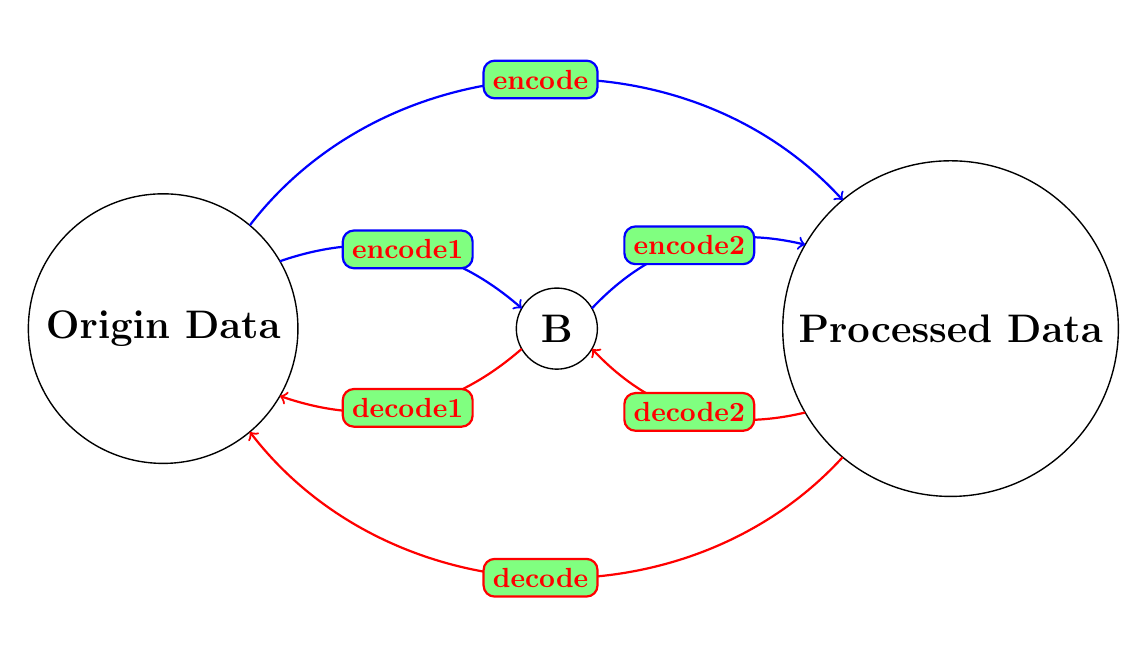
\begin{tikzpicture}
  \SetGraphUnit{5}
  \Vertex{B}
  \WE(B){Origin Data}
  \EA(B){Processed Data}
  \Edge[label = encode1,color = blue](Origin Data)(B)
  \Edge[label = encode2,color = blue](B)(Processed Data)
  \Edge[label = decode2,color = red](Processed Data)(B)
  \Edge[label = decode1,color = red](B)(Origin Data)
  \tikzset{EdgeStyle/.append style = {bend left = 50}}
  \Edge[label = encode,color=blue](Origin Data)(Processed Data)
  \Edge[label = decode,color=red](Processed Data)(Origin Data)
\end{tikzpicture}

\begin{python}
import tensorflow as tf
import matplotlib.pyplot as plt
data_path = '/home/hpc/文档/mnist_tutorial/mnist'

from tensorflow.examples.tutorials.mnist import input_data
mnist = input_data.read_data_sets(data_path, one_hot=False)


# Visualize decoder setting
learning_rate = 0.01
training_epochs = 5
batch_size = 256
display_step = 1
examples_to_show = 10

n_input = 784  # MNIST data input (img shape: 28*28)

x = tf.placeholder(tf.float32,[None,n_input])

n_hidden_1 = 256
n_hidden_2 = 128
weights = {
    'encode_h1':tf.Variable(tf.random_normal([n_input,n_hidden_1])),
    'encode_h2':tf.Variable(tf.random_normal([n_hidden_1,n_hidden_2])),
    'decode_h2':tf.Variable(tf.random_normal([n_hidden_2,n_hidden_1])),
    'decode_h1':tf.Variable(tf.random_normal([n_hidden_1,n_input]))
}
bias = {'encode_h1':tf.Variable(tf.random_normal([n_hidden_1])),
    'encode_h2':tf.Variable(tf.random_normal([n_hidden_2])),
    'decode_h2':tf.Variable(tf.random_normal([n_hidden_1])),
    'decode_h1':tf.Variable(tf.random_normal([n_input]))

}
def encode(x):
    layer_1 = tf.nn.sigmoid(tf.add(tf.matmul(x,weights['encode_h1']),bias['encode_h1']))
    layer_2 = tf.nn.sigmoid(tf.add(tf.matmul(layer_1,weights['encode_h2']),bias['encode_h2']))
    return layer_2

def decode(x):
    layer_1 = tf.nn.sigmoid(tf.add(tf.matmul(x,weights['decode_h2']),bias['decode_h2']))
    layer_2 = tf.nn.sigmoid(tf.add(tf.matmul(layer_1,weights['decode_h1']),bias['decode_h1']))
    return layer_2



encode_op = encode(x)
decode_op = decode(encode_op)
y_pred = decode_op
y_true = x
cost = tf.reduce_mean(tf.square(y_pred-y_true))
optimizer = tf.train.AdamOptimizer(learning_rate).minimize(cost)

with tf.Session() as sess:
    init = tf.global_variables_initializer()
    sess.run(init)
    total_batch = int(mnist.train.num_examples/batch_size)
    for epoch in range(training_epochs):
        for i in range(total_batch):
            batch_xs,batch_ys = mnist.train.next_batch(batch_size)
            _, c = sess.run([optimizer, cost], feed_dict={x: batch_xs})
        if epoch%display_step==0:
            print("Epoch:",'%04d'%(epoch+1),'cost=','{:.9f}'.format(c))
    print('Optimize finish')
    encode_decode = sess.run(y_pred,feed_dict={x:mnist.test.images[:examples_to_show]})
    f,a = plt.subplots(2,10,figsize=(10,2))
    for i in range(examples_to_show):
        a[0][i].imshow(sess.run(tf.reshape(mnist.test.images[i],[28,28])))
        a[1][i].imshow(sess.run(tf.reshape(encode_decode[i],[28,28])))
    plt.savefig('auto_encode.png',dpi=800)
\end{python}
\begin{center}
\begin{figure}[H]
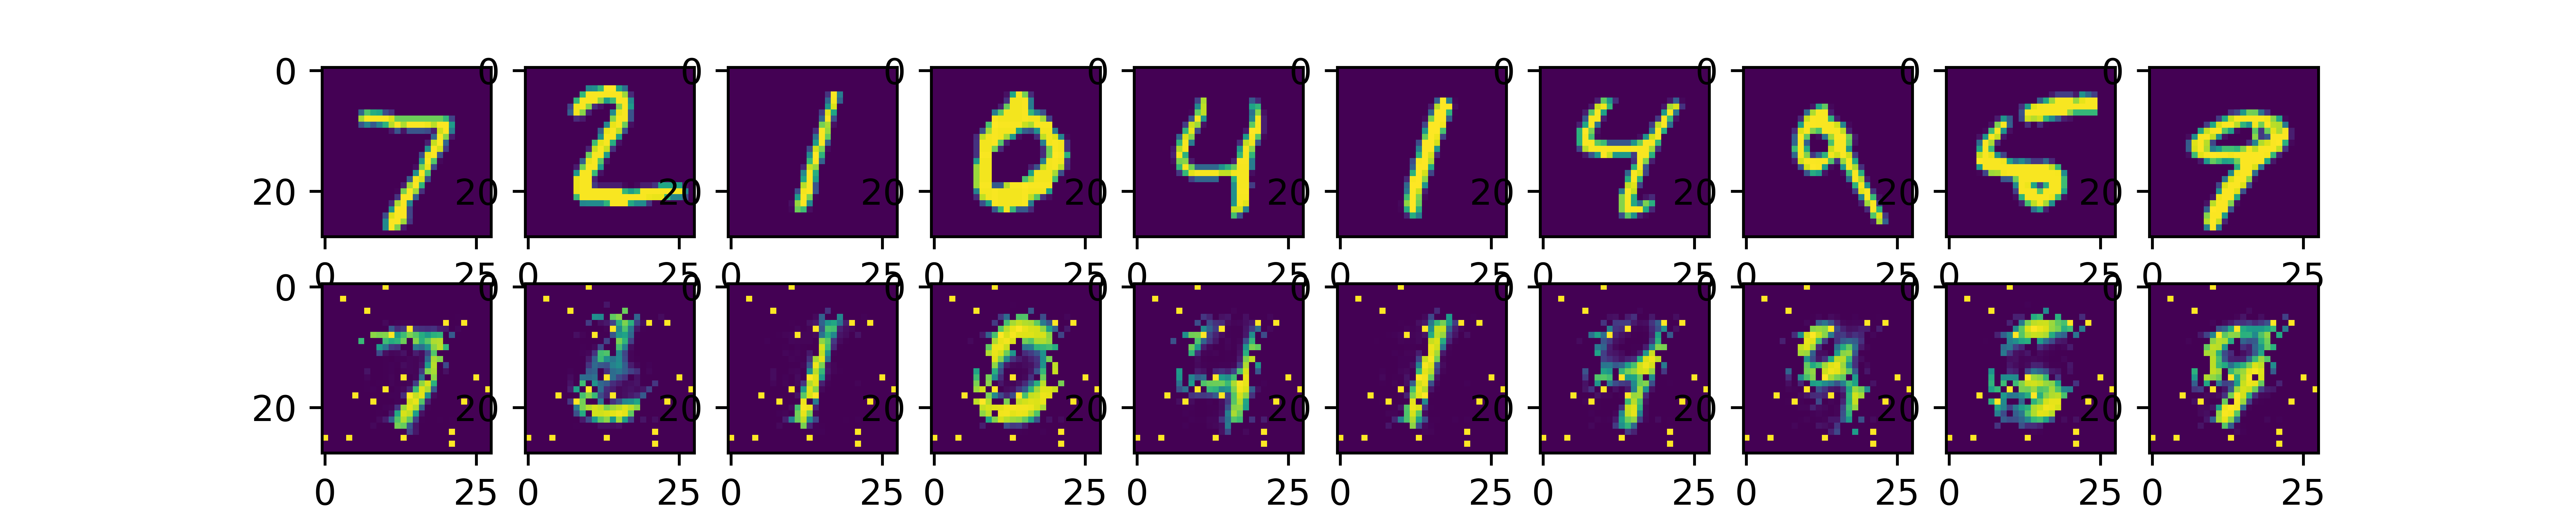
\includegraphics[scale=0.5]{auto_encode.png}
\caption{原图和自编码解码后的图像}
\end{figure}
\end{center}
编码器输出可视化:
\begin{python}
import tensorflow as tf
import matplotlib.pyplot as plt

from tensorflow.examples.tutorials.mnist import input_data
path = '/home/hpc/文档/mnist_tutorial/mnist'
mnist = input_data.read_data_sets(path, one_hot=False)

learning_rate = 0.01
training_epochs = 5
batch_size = 256
display_step = 1
examples_to_show = 10

n_input = 784  # MNIST data input (img shape: 28*28)

X = tf.placeholder("float", [None, n_input])

n_hidden_1 = 256 # 1st layer num features
n_hidden_2 = 128 # 2nd layer num features

learning_rate = 0.01    # 0.01 this learning rate will be better! Tested
training_epochs = 10
batch_size = 256
display_step = 1
n_input = 784  # MNIST data input (img shape: 28*28)
X = tf.placeholder("float", [None, n_input])
n_hidden_1 = 128
n_hidden_2 = 64
n_hidden_3 = 10
n_hidden_4 = 2
weights = {
    'encoder_h1': tf.Variable(tf.truncated_normal([n_input, n_hidden_1],)),
    'encoder_h2': tf.Variable(tf.truncated_normal([n_hidden_1, n_hidden_2],)),
    'encoder_h3': tf.Variable(tf.truncated_normal([n_hidden_2, n_hidden_3],)),
    'encoder_h4': tf.Variable(tf.truncated_normal([n_hidden_3, n_hidden_4],)),
    'decoder_h1': tf.Variable(tf.truncated_normal([n_hidden_4, n_hidden_3],)),
    'decoder_h2': tf.Variable(tf.truncated_normal([n_hidden_3, n_hidden_2],)),
    'decoder_h3': tf.Variable(tf.truncated_normal([n_hidden_2, n_hidden_1],)),
    'decoder_h4': tf.Variable(tf.truncated_normal([n_hidden_1, n_input],)),
}
biases = {
    'encoder_b1': tf.Variable(tf.random_normal([n_hidden_1])),
    'encoder_b2': tf.Variable(tf.random_normal([n_hidden_2])),
    'encoder_b3': tf.Variable(tf.random_normal([n_hidden_3])),
    'encoder_b4': tf.Variable(tf.random_normal([n_hidden_4])),
    'decoder_b1': tf.Variable(tf.random_normal([n_hidden_3])),
    'decoder_b2': tf.Variable(tf.random_normal([n_hidden_2])),
    'decoder_b3': tf.Variable(tf.random_normal([n_hidden_1])),
    'decoder_b4': tf.Variable(tf.random_normal([n_input])),
}
def encoder(x):
    layer_1 = tf.nn.sigmoid(tf.add(tf.matmul(x, weights['encoder_h1']),
                                   biases['encoder_b1']))
    layer_2 = tf.nn.sigmoid(tf.add(tf.matmul(layer_1, weights['encoder_h2']),
                                   biases['encoder_b2']))
    layer_3 = tf.nn.sigmoid(tf.add(tf.matmul(layer_2, weights['encoder_h3']),
                                   biases['encoder_b3']))
    layer_4 = tf.add(tf.matmul(layer_3, weights['encoder_h4']),
                                    biases['encoder_b4'])
    return layer_4
def decoder(x):
    layer_1 = tf.nn.sigmoid(tf.add(tf.matmul(x, weights['decoder_h1']),
                                   biases['decoder_b1']))
    layer_2 = tf.nn.sigmoid(tf.add(tf.matmul(layer_1, weights['decoder_h2']),
                                   biases['decoder_b2']))
    layer_3 = tf.nn.sigmoid(tf.add(tf.matmul(layer_2, weights['decoder_h3']),
                                biases['decoder_b3']))
    layer_4 = tf.nn.sigmoid(tf.add(tf.matmul(layer_3, weights['decoder_h4']),
                                biases['decoder_b4']))
    return layer_4

encoder_op = encoder(X)
decoder_op = decoder(encoder_op)

y_pred = decoder_op
y_true = X

cost = tf.reduce_mean(tf.pow(y_true - y_pred, 2))
optimizer = tf.train.AdamOptimizer(learning_rate).minimize(cost)


with tf.Session() as sess:
    init = tf.global_variables_initializer()
    sess.run(init)
    total_batch = int(mnist.train.num_examples/batch_size)
    for epoch in range(training_epochs):
        for i in range(total_batch):
            batch_xs, batch_ys = mnist.train.next_batch(batch_size)  # max(x) = 1, min(x) = 0
            _, c = sess.run([optimizer, cost], feed_dict={X: batch_xs})
        if epoch % display_step == 0:
            print("Epoch:", '%04d' % (epoch+1),
                  "cost=", "{:.9f}".format(c))
    print("Optimization Finished!")
    encode_decode = sess.run(
        y_pred, feed_dict={X: mnist.test.images[:examples_to_show]})
    encoder_result = sess.run(encoder_op, feed_dict={X: mnist.test.images})
    plt.scatter(encoder_result[:, 0], encoder_result[:, 1], c=mnist.test.labels)
    plt.title('encode output')
    plt.colorbar()
    plt.savefig('auto_encode_v.png',dpi=800)
\end{python}

\begin{center}
\begin{figure}[H]
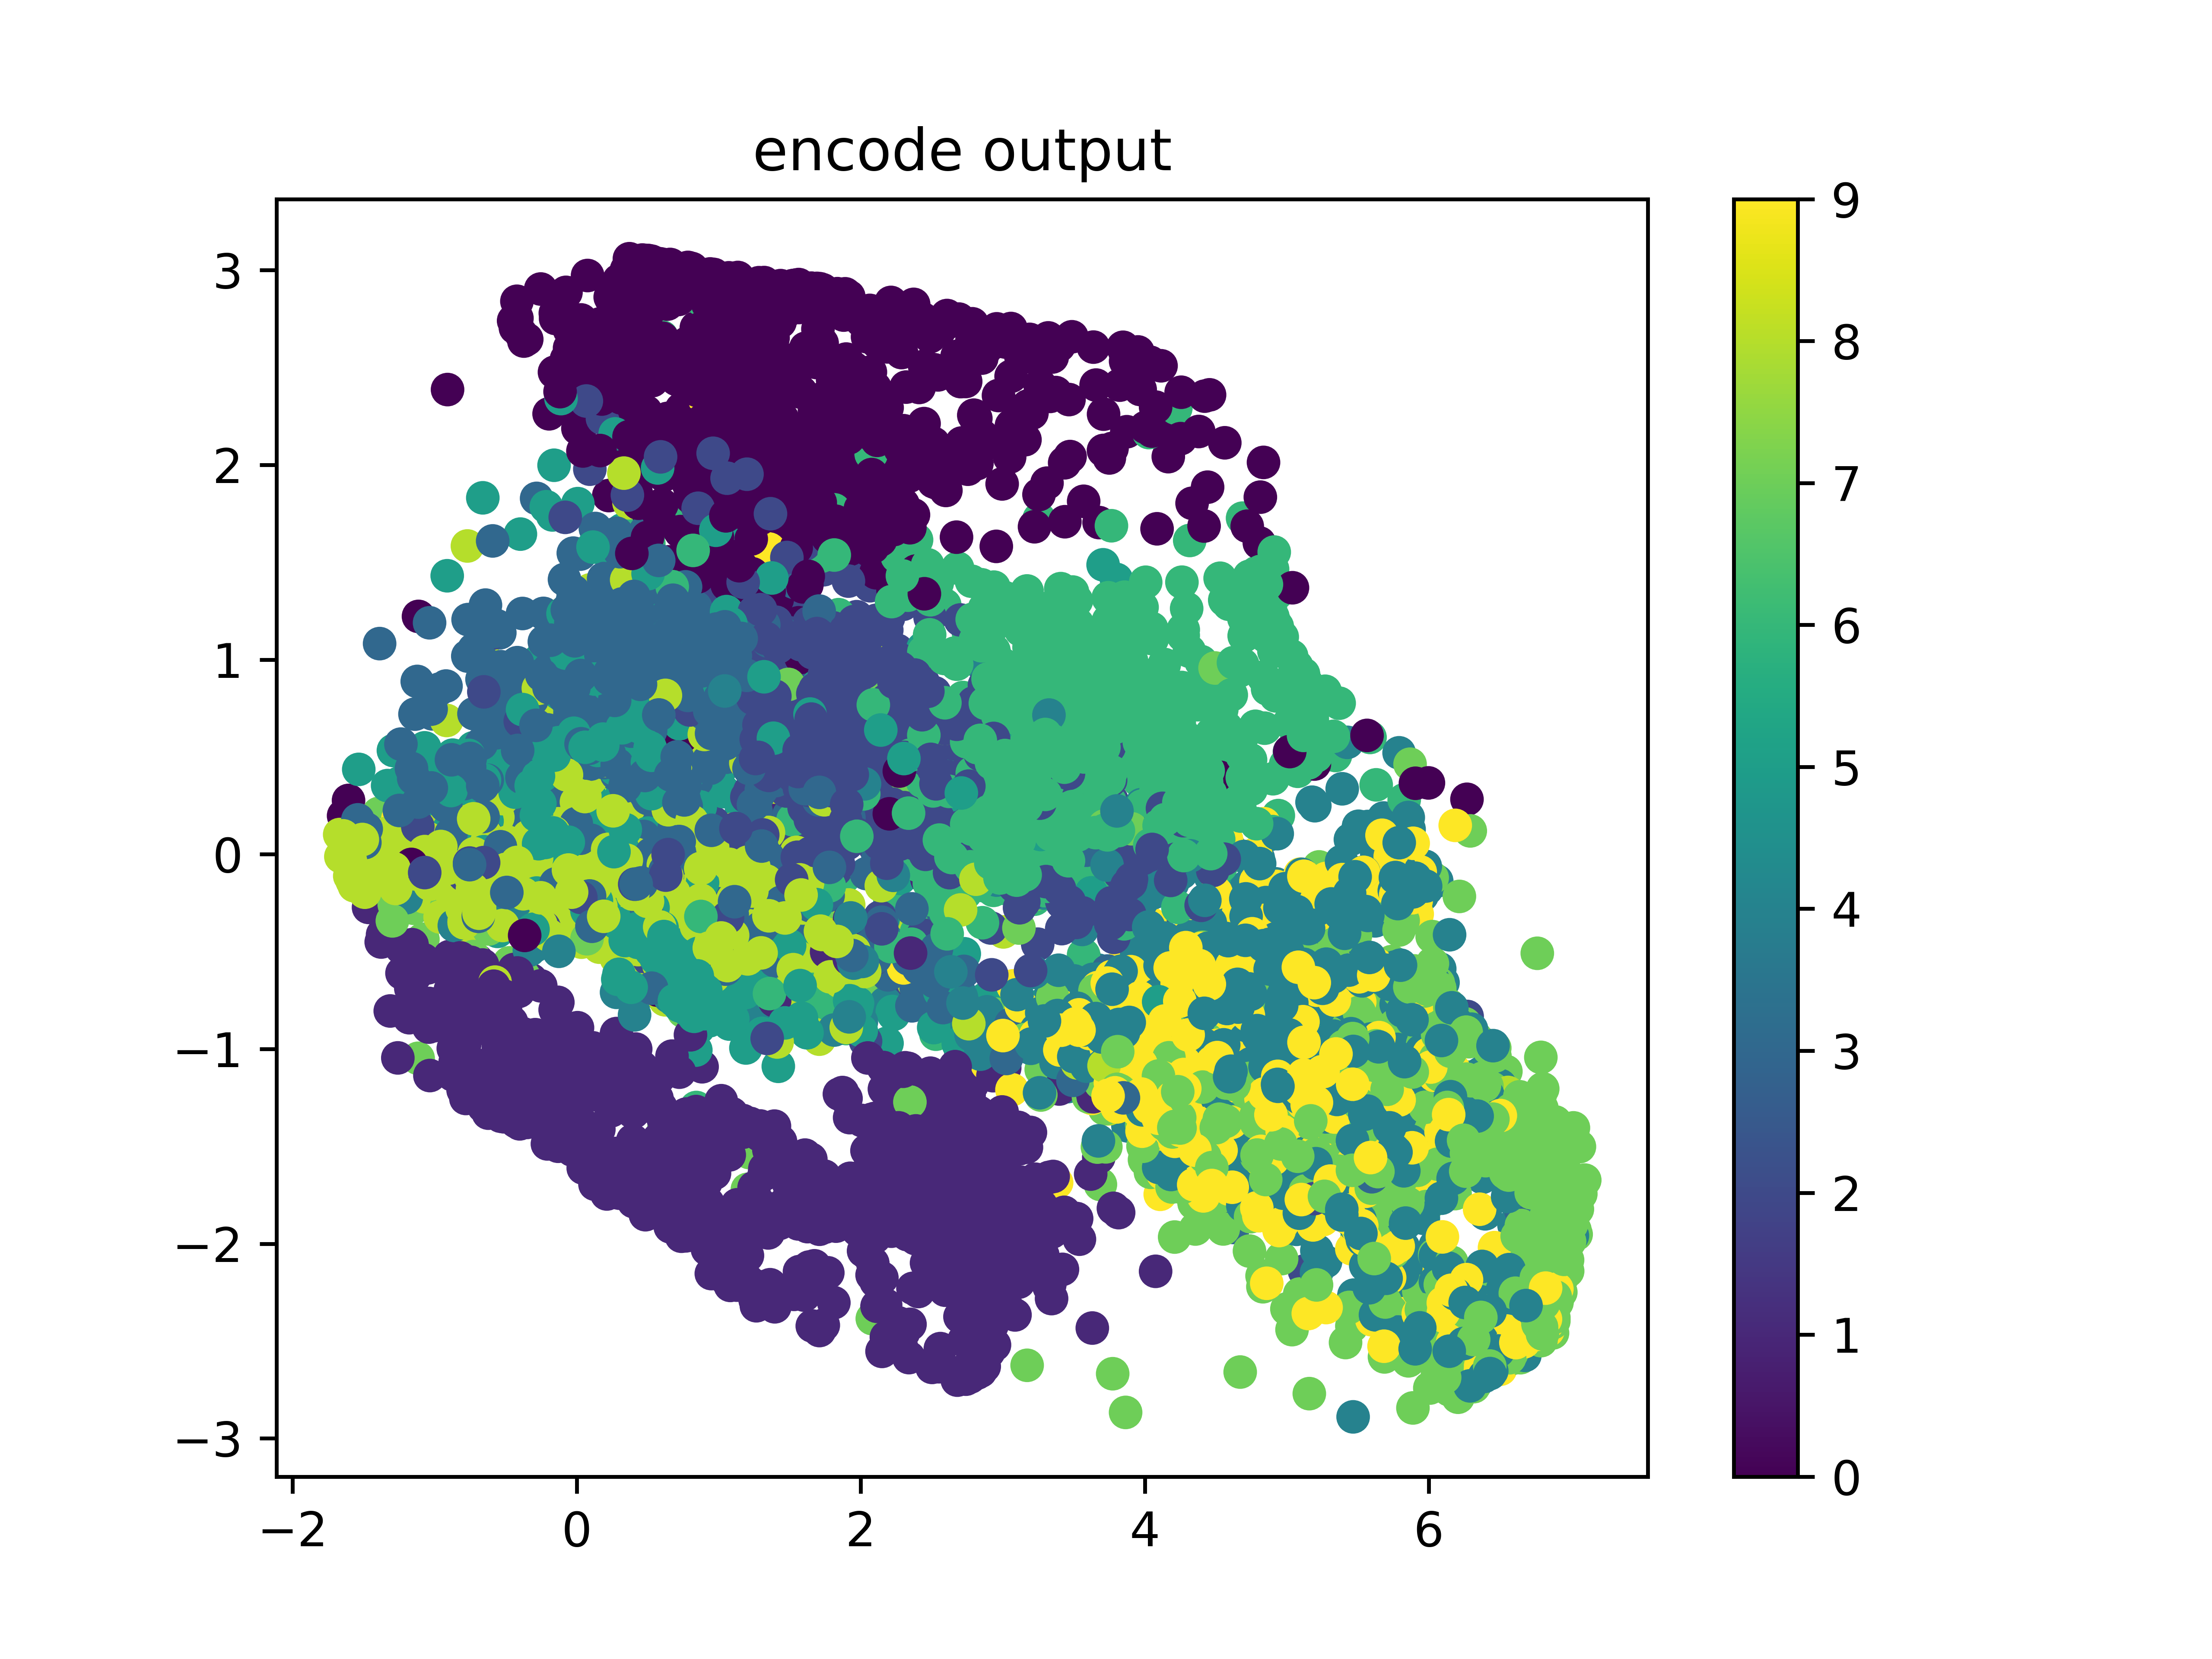
\includegraphics[scale=0.7]{auto_encode_v.png}
\end{figure}
\end{center}
\section{稀疏编码}
稀疏编码算法是一种无监督学习方法,它用来寻找一组“超完备”基向量来更高效地表示样本数据。稀疏编码算法的目的就是找到一组基向量 $\mathbf{\phi}_i$ ,使得我们能将输入向量 $\mathbf{x}$ 表示为这些基向量的线性组合:
\begin{align}
\mathbf{x} = \sum_{i=1}^k a_i \mathbf{\phi}_{i} 
\end{align}
虽然形如主成分分析技术(PCA)能使我们方便地找到一组“完备”基向量,但是这里我们想要做的是找到一组“超完备”基向量来表示输入向量 $\mathbf{x}\in\mathbb{R}^n$ (也就是说,k > n)。超完备基的好处是它们能更有效地找出隐含在输入数据内部的结构与模式。然而,对于超完备基来说,系数 ai 不再由输入向量 $\mathbf{x}$ 唯一确定。因此,在稀疏编码算法中,我们另加了一个评判标准“稀疏性”来解决因超完备而导致的退化(degeneracy)问题。

这里,我们把“稀疏性”定义为:只有很少的几个非零元素或只有很少的几个远大于零的元素。要求系数$a_i$ 是稀疏的意思就是说:对于一组输入向量,我们只想有尽可能少的几个系数远大于零。选择使用具有稀疏性的分量来表示我们的输入数据是有原因的,因为绝大多数的感官数据,比如自然图像,可以被表示成少量基本元素的叠加,在图像中这些基本元素可以是面或者线。同时,比如与初级视觉皮层的类比过程也因此得到了提升。

我们把有 m 个输入向量的稀疏编码代价函数定义为:
\begin{align}
\text{minimize}_{a^{(j)}_i,\mathbf{\phi}_{i}} \sum_{j=1}^{m} \left|\left| \mathbf{x}^{(j)} - \sum_{i=1}^k a^{(j)}_i \mathbf{\phi}_{i}\right|\right|^{2} + \lambda \sum_{i=1}^{k}S(a^{(j)}_i)
\end{align}

此处 S(.) 是一个稀疏代价函数,由它来对远大于零的 ai 进行“惩罚”。我们可以把稀疏编码目标函式的第一项解释为一个重构项,这一项迫使稀疏编码算法能为输入向量 $\mathbf{x}$ 提供一个高拟合度的线性表达式,而公式第二项即“稀疏惩罚”项,它使 $\mathbf{x}$ 的表达式变得“稀疏”。常量 λ 是一个变换量,由它来控制这两项式子的相对重要性。

虽然“稀疏性”的最直接测度标准是 "L0" 范式$(S(a_i) = \mathbf{1}(|a_i|>0))$,但这是不可微分的,而且通常很难进行优化。在实际中,稀疏代价函数 S(.) 的普遍选择是L1 范式代价函数 $S(a_i)=\left|a_i\right|_1$  及对数代价函数 $S(a_i)=\log(1+a_i^2)$ 。

此外,很有可能因为减小 $a_i$ 或增加 $\mathbf{\phi}_i$ 至很大的常量,使得稀疏惩罚变得非常小。为防止此类事件发生,我们将限制 $\left|\left|\mathbf{\phi}\right|\right|^2$ 要小于某常量 C 。包含了限制条件的稀疏编码代价函数的完整形式如下:
\begin{equation}
\text{minimize}_{a_i^{(j)},\phi_i}\Sigma_j=1^m\|x^{(j)}-\Sigma_{i=1}^ka_i^{(j)}\phi_i\|^2+\lambda\Sigma_{i=1}^kS(s_i^{(j)})\quad\|\phi_i\|^2\leq C,\forall i=1,\ldots,k
\end{equation}
\subsection{稀疏编码的概率表示}
到目前为止,我们所考虑的稀疏编码,是为了寻找到一个稀疏的、超完备基向量集,来覆盖我们的输入数据空间。现在换一种方式,我们可以从概率的角度出发,将稀疏编码算法当作一种“生成模型”。

我们将自然图像建模问题看成是一种线性叠加,叠加元素包括 k 个独立的源特征 $\mathbf{\phi}_i$ 以及加性噪声 ν :
\begin{align}
\mathbf{x} = \sum_{i=1}^k a_i \mathbf{\phi}_{i} + \nu(\mathbf{x})
\end{align}

我们的目标是找到一组特征基向量 $\mathbf{\phi}$ ,它使得图像的分布函数 $P(\mathbf{x}\mid\mathbf{\phi})$ 尽可能地近似于输入数据的经验分布函数 $P^*(\mathbf{x})$ 。一种实现方式是,最小化 $P^*(\mathbf{x})$ 与 $P(\mathbf{x}\mid\mathbf{\phi})$ 之间的 KL 散度,此 KL 散度表示如下:
\begin{align}
D(P^*(\mathbf{x})||P(\mathbf{x}\mid\mathbf{\phi})) = \int P^*(\mathbf{x}) \log \left(\frac{P^*(\mathbf{x})}{P(\mathbf{x}\mid\mathbf{\phi})}\right)d\mathbf{x}
\end{align}

因为无论我们如何选择 $\mathbf{\phi}$ ,经验分布函数 $P^*(\mathbf{x})$ 都是常量,也就是说我们只需要最大化对数似然函数 $P(\mathbf{x}\mid\mathbf{\phi})$ 。 假设v是具有方差$\sigma^2$的高斯白噪声,则有下式:
\begin{align}
P(\mathbf{x} \mid \mathbf{a}, \mathbf{\phi}) = \frac{1}{Z} \exp\left(- \frac{(\mathbf{x}-\sum^{k}_{i=1} a_i \mathbf{\phi}_{i})^2}{2\sigma^2}\right)
\end{align}

为了确定分布 $P(\mathbf{x}\mid\mathbf{\phi})$ ,我们需要指定先验分布 $P(\mathbf{a})$ 。假定我们的特征变量是独立的,我们就可以将先验概率分解为:
\begin{align}
P(\mathbf{a}) = \prod_{i=1}^{k} P(a_i)
\end{align}

此时,我们将“稀疏”假设加入进来——假设任何一幅图像都是由相对较少的一些源特征组合起来的。因此,我们希望$a_i$的概率分布在零值附近是凸起的,而且峰值很高。一个方便的参数化先验分布就是:
\begin{align}
P(a_i) = \frac{1}{Z}\exp(-\beta S(a_i))
\end{align}

这里$S(a_i)$是决定先验分布的形状的函数。

当定义了 $P(\mathbf{x} \mid \mathbf{a} , \mathbf{\phi})$ 和  $P(\mathbf{a})$ 后,我们就可以写出在由 $\mathbf{\phi}$ 定义的模型之下的数据 $\mathbf{x}$ 的概率分布:
\begin{align}
P(\mathbf{x} \mid \mathbf{\phi}) = \int P(\mathbf{x} \mid \mathbf{a}, \mathbf{\phi}) P(\mathbf{a}) d\mathbf{a}
\end{align}

那么,我们的问题就简化为寻找:
\begin{align}
\mathbf{\phi}^*=\text{argmax}_{\mathbf{\phi}} < \log(P(\mathbf{x} \mid \mathbf{\phi})) >
\end{align}

这里 < . > 表示的是输入数据的期望值。

不幸的是,通过对 $\mathbf{a}$ 的积分计算 $P(\mathbf{x} \mid \mathbf{\phi})$ 通常是难以实现的。虽然如此,我们注意到如果$ P(\mathbf{x} \mid \mathbf{\phi}) $的分布(对于相应的 $\mathbf{a}$ )足够陡峭的话,我们就可以用$ P(\mathbf{x} \mid \mathbf{\phi})$ 的最大值来估算以上积分。估算方法如下:
\begin{align}
\mathbf{\phi}^{*'}=\text{argmax}_{\mathbf{\phi}} < \max_{\mathbf{a}} \log(P(\mathbf{x} \mid \mathbf{\phi})) >
\end{align}

跟之前一样,我们可以通过减小$a_i$或增大 $\mathbf{\phi}$ 来增加概率的估算值(因为$P(a_i)$在零值附近陡升)。因此我们要对特征向量 $\mathbf{\phi}$ 加一个限制以防止这种情况发生。
最后,我们可以定义一种线性生成模型的能量函数,从而将原先的代价函数重新表述为:
\begin{align}
E(x,a|\phi):=&-log(P(x|\phi,\mathbf{a})P(\mathbf{a}))\\
            =&\Sigma_{j=1}^m\|x^{(j)}-\Sigma_{i=1}^k\alpha_i^{(j)}\phi_j\|^2+\lambda\Sigma_{i=1}^{k}S(\alpha_i^{(j)})
\end{align}
其中$\lambda = 2\sigma2\beta$ ,并且关系不大的常量已被隐藏起来。因为最大化对数似然函数等同于最小化能量函数,我们就可以将原先的优化问题重新表述为:
\begin{equation}
\mathbf{\phi}^{*},\mathbf{a}^{*}=\text{argmin}_{\mathbf{\phi},\mathbf{a}} \sum_{j=1}^{m} \left|\left| \mathbf{x}^{(j)} - \sum_{i=1}^k a^{(j)}_i \mathbf{\phi}_{i}\right|\right|^{2} + \lambda \sum_{i=1}^{k}S(a^{(j)}_i) 
\end{equation}
使用概率理论来分析,我们可以发现,选择 L1 惩罚和 $\log(1+a_i^2)$ 惩罚作为函数 S(.) ,分别对应于使用了拉普拉斯概率 $P(a_i) \propto \exp\left(-\beta|a_i|\right)$ 和柯西先验概率 $P(a_i) \propto \frac{\beta}{1+a_i^2}$ 。
\section{PCA}
在多元统计分析中,主成分分析(英语:Principal components analysis,PCA)是一种分析、简化数据集的技术。主成分分析经常用于减少数据集的维数,同时保持数据集中的对方差贡献最大的特征。这是通过保留低阶主成分,忽略高阶主成分做到的。这样低阶成分往往能够保留住数据的最重要方面。但是,这也不是一定的,要视具体应用而定。由于主成分分析依赖所给数据,所以数据的准确性对分析结果影响很大。
主成分分析由卡尔·皮尔逊于1901年发明[1],用于分析数据及建立数理模型。其方法主要是通过对协方差矩阵进行特征分解[2],以得出数据的主成分(即特征向量)与它们的权值(即特征值[3])。PCA是最简单的以特征量分析多元统计分布的方法。其结果可以理解为对原数据中的方差做出解释:哪一个方向上的数据值对方差的影响最大?换而言之,PCA提供了一种降低数据维度的有效办法;如果分析者在原数据中除掉最小的特征值所对应的成分,那么所得的低维度数据必定是最优化的(也即,这样降低维度必定是失去讯息最少的方法)。主成分分析在分析复杂数据时尤为有用,比如人脸识别。
PCA是最简单的以特征量分析多元统计分布的方法。通常情况下,这种运算可以被看作是揭露数据的内部结构,从而更好的解释数据的变量的方法。如果一个多元数据集能够在一个高维数据空间坐标系中被显现出来,那么PCA就能够提供一幅比较低维度的图像,这幅图像即为在讯息最多的点上原对象的一个‘投影’。这样就可以利用少量的主成分使得数据的维度降低了。
PCA跟因子分析密切相关,并且已经有很多混合这两种分析的统计包。而真实要素分析则是假定底层结构,求得微小差异矩阵的特征向量。
\subsection{数学定义}
PCA的数学定义是:一个正交化线性变换,把数据变换到一个新的坐标系统中,使得这一数据的任何投影的第一大方差在第一个坐标(称为第一主成分)上,第二大方差在第二个坐标(第二主成分)上,依次类推。
定义一个$n\times m$的矩阵, $X^T$为去平均值(以平均值为中心移动至原点)的数据,其行为数据样本,列为数据类别(注意,这里定义的是XT 而不是X)。则X的奇异值分解为$X = W\Sigma V^T$,其中$m\times m$矩阵W是$XX^T$的本征矢量矩阵,$\Sigma$是$m\times n$的非负矩形对角矩阵,V是$m\times n$的$X^TX$的本征矢量矩阵。据此,
\begin{equation}
\begin{aligned}
\mathbf{Y}^T&=\mathbf{X}^{T}\mathbf{W}\\
            &=\mathbf{V}{\Sigma}^{T}\mathbf{W}^{T}\mathbf{W}\\
            &=\mathbf{V}{\Sigma}^{T}
\end{aligned}
\end{equation}
当 $m < n − 1$时,$V$ 在通常情况下不是唯一定义的,而$Y$ 则是唯一定义的。$W$ 是一个正交矩阵,$Y^T$是$X^T$的转置,且$Y^T$的第一列由第一主成分组成,第二列由第二主成分组成,依此类推。
为了得到一种降低数据维度的有效办法,我们可以利用$W_L$把 X 映射到一个只应用前面L个向量的低维空间中去:
\begin{equation}
\mathbf{Y} =\mathbf{W_{L}}^{T}\mathbf{X} ={\Sigma _{L}}\mathbf {V} ^{T}
\end{equation}
其中 ${\Sigma _{L}} =\mathbf{I} _{L\times m}{\Sigma }$且$\mathbf{I} _{L\times m} $为$ L\times m L\times m$的单位矩阵。
X 的单向量矩阵W相当于协方差矩阵的本征矢量 $C=XX^T$,
\begin{equation}
XX^T = W\Sigma\Sigma^TW^T
\end{equation}
在欧几里得空间给定一组点数,第一主成分对应于通过多维空间平均点的一条线,同时保证各个点到这条直线距离的平方和最小。去除掉第一主成分后,用同样的方法得到第二主成分。依此类推。在Σ中的奇异值均为矩阵 $XX^T$的本征值的平方根。每一个本征值都与跟它们相关的方差是成正比的,而且所有本征值的总和等于所有点到它们的多维空间平均点距离的平方和。PCA提供了一种降低维度的有效办法,本质上,它利用正交变换将围绕平均点的点集中尽可能多的变量投影到第一维中去,因此,降低维度必定是失去讯息最少的方法。PCA具有保持子空间拥有最大方差的最优正交变换的特性。然而,当与离散余弦变换相比时,它需要更大的计算需求代价。非线性降维技术相对于PCA来说则需要更高的计算要求。
PCA对变量的缩放很敏感。如果我们只有两个变量,而且它们具有相同的样本方差,并且成正相关,那么PCA将涉及两个变量的主成分的旋转。但是,如果把第一个变量的所有值都乘以100,那么第一主成分就几乎和这个变量一样,另一个变量只提供了很小的贡献,第二主成分也将和第二个原始变量几乎一致。这就意味着当不同的变量代表不同的单位(如温度和质量)时,PCA是一种比较武断的分析方法。但是在Pearson的题为 "On Lines and Planes of Closest Fit to Systems of Points in Space"的原始文件里,是假设在欧几里得空间里不考虑这些。一种使PCA不那么武断的方法是使用变量缩放以得到单位方差。

\chapter{Tensorflow基础}
\section{Tensorflow基础概念}
在Tensorflow中正如它的名字显示的定义tensor计算。一个tensor是一个概括的矩阵和向量,并且有能力表示更高的维度,我们写Tensorflow程序,主要的对象就是tf.Tensor,一个tensor定义计算的一部分最后生成值。TensorFlow程序首先用tensor建立一个图,然后运行图获得想要的数据。一个tensor需要指定两个参数:数据类型和形状。Tensor中的数据类型相同,而且总是可知的,形状可能仅仅部分知道。
下面是一些特殊的Tensor类型:
\begin{itemize}
\item	tf.Variable
\item	tf.Constant
\item	tf.Placeholder
\item	tf.SparseTensor
\end{itemize}
\subsection{Rank}
tf.Tensor的rank是对象的维度。TensorFlow的rank和数学中矩阵的rank不一样,下面显示TensorFlow rank和相对应的数学实体
\begin{center}
\begin{tabular}{|c|c|}
\hline
rank&数学实体\\
\hline
0&Scalar(只有值)\\
\hline
1&Vecor(值和方向)\\
\hline
2&矩阵(数值表)\\
\hline
3&3-Tensor\\
\hline
n&n-Tensor\\
\hline
\end{tabular}
\end{center}
\textbf{rank0}

下面片段展示创建一些0维的变量。
\begin{python}
mammal = tf.Variable("Elephant", tf.string)
ignition = tf.Variable(451, tf.int16)
floating = tf.Variable(3.14159265359, tf.float64)
its_complicated = tf.Variable((12.3, -4.85), tf.complex64)
\end{python}
\textbf{Rank1}
传递列表作为初始值创建1维tf.Tensor对象
\begin{python}
mystr = tf.Variable(["Hello"], tf.string)
cool_numbers  = tf.Variable([3.14159, 2.71828], tf.float32)
first_primes = tf.Variable([2, 3, 5, 7, 11], tf.int32)
its_very_complicated = tf.Variable([(12.3, -4.85), (7.5, -6.23)], tf.complex64)
\end{python}
\textbf{更高的rank}
二维的Tensor至少有一行一列
\begin{python}
mymat = tf.Variable([[7],[11]], tf.int16)
myxor = tf.Variable([[False, True],[True, False]], tf.bool)
linear_squares = tf.Variable([[4], [9], [16], [25]], tf.int32)
squarish_squares = tf.Variable([ [4, 9], [16, 25] ], tf.int32)
rank_of_squares = tf.rank(squarish_squares)
mymatC = tf.Variable([[7],[11]], tf.int32)
\end{python}
更高rank的Tensor,有n维数组。例如在图像处理,一些tensor的rank为4,维度通常是example-in-batch,image width,image height,color chennel。
\begin{python}
my_image = tf.zeros([10, 299, 299, 3])  # batch x height x width x color
\end{python}
\subsection{获取Tensor对象的rank}
你可以使用tf.rank方法获取tensor对象的rank。例如下面获取my3d的rank。
\begin{python}
r = tf.rank(my2d)#在图运行后,r将保持值3。
\end{python}
\subsection{Tensor的切片}
因为tf.Tensor是n维cell阵列,为了访问tf.Tensor的单个cell,你需要指定索引。
对于rank为0的tensor,不需要索引,因为它已经是单个值了。\par
对于rank1(向量),传递一个索引允许你访问:
\begin{python}
my_scale = my_vector[2]
\end{python}
如果你想动态的选择向量中的元素,你可以指定[]一个tf.Tensor。
传递一个数值访问矩阵的子向量:
\begin{python}
my_row_vetor = my_matrix[2]
my_column_vector = my_matrix[:, 3]
\end{python}
\subsection{形状}
shape是tensor每一维元素的个数。TensorFlow在构造图的时候自动计算形状。有时候自动计算可能不知道rank,如果rank已经知道,每一维的形状可能直到可能不知道。
\begin{tabular}{|c|c|c|c|}
\hline
rank&shape&维数&example\\
\hline
0&[]&0-D&O维Tensor,标量\\
\hline
1&[D0]&1-D&一维tensor的形状\\
\hline
2&[D0,D1]&2-D&二维Tensoe的形状\\
\hline
3&[D0,D1,D2]&3-D&三维Tensor的形状\\
\hline
n&[D0,D1,\ldots,$D_{n-1}$]&N维tensor的形状[$D_0,D_1,\ldots,D_{n-1}$]&\\
\hline
\end{tabular}
\subsection{获取tf.Tensor对象的形状}
当建立图的时候tensor的形状已知是很有用的,你可以通过tensor的shape属性得到。得到完全定义的tf.Tensor的形状可以使用Tf.shape操作。这个方法你可以建立一个图操作tensor的形状。

例如,这里是如何如何创建一个和给定矩阵列数相同的全零向量。
\begin{python}
zeros = tf.zeros(tf.shape(my_matrix)[1])
\end{python}
\subsection{改变Tensor的形状}
tensor的元素是所有形状值的乘积。标量的元素总是1.因此,因为有相同元素不同形状的tensor,转变他们的形状是很方便的。可以使用tf.reshape.

下面例子展示了如何reshape tensor。
\begin{python}
rank_three_tensor = tf.ones([3, 4, 5])
matrix = tf.reshape(rank_three_tensor, [6, 10])  # Reshape existing content into
                                                 # a 6x10 matrix
matrixB = tf.reshape(matrix, [3, -1])  #  Reshape existing content into a 3x20
                                       # matrix. -1 tells reshape to calculate
                                       # the size of this dimension.
matrixAlt = tf.reshape(matrixB, [4, 3, -1])  # Reshape existing content into a
                                             #4x3x5 tensor

# Note that the number of elements of the reshaped Tensors has to match the
# original number of elements. Therefore, the following example generates an
# error because no possible value for the last dimension will match the number
# of elements.
yet_another = tf.reshape(matrixAlt, [13, 2, -1])  # ERROR!
\end{python}
\subsection{数据类型}
tf.Tensor不可能有一个以上的数据类型。然而序列化数据结构作为字符串尺寸处在tf.Tensor里是可能的。

可以使用tf.cast转换一种数据类型到另一种。
\begin{python}
# Cast a constant integer tensor into floating point.
float_tensor = tf.cast(tf.constant([1, 2, 3]), dtype=tf.fl
\end{python}
通过Tensor的dtype查看tensor的数据类型。你通过python对象创建tf.Tensor的时候需要指定数据类型。如果你不指定TensorFlow选择一个代表你数据的数据类型。TensorFlow转换Python整数为tf.int32,浮点数为tf.float32。转换数组时TensorFlow用和numpy相同的规则。
\subsection{计算Tensor}
当计算图被创建后你可以通过运行计算tf.Tensor获取指定的值。用Tensor.eval方法简单的计算:
\begin{python}
constant = tf.constant([1,2,3])
tensor = constant*constant
print(tensor.eval())
\end{python}
eval方法仅仅当tf.Session()被激活时可用。Tensor.eval然后会得到一个一个和tensor相同内容的numpy数组。有时候没有上下文计算tf.Tensor是不可能的。例如,tensor依赖于Placeholder在提供给Placeholder值之前不能计算。
\begin{python}
p = tf.placeholder(tf.float32)
t = p + 1.0
t.eval()  # This will fail, since the placeholder did not get a value.
t.eval(feed_dict={p:2.0})  # This will succeed because we're feeding a value
                           # to the placeholder.
\end{python}
其他的模型结构在计算tf.Tensor时可能很复杂。TensorFlow不能直接计算定义在函数内部的或者控制流结构的tf.Tensor。如果tf.Tensor伊奈于队列中的值,计算tf.Tensorbang仅仅入队的时候工作,负责计算被挂起。当和queue工作的时候,记得在计算任何tf.Tensor之前用tf.train.start\_queue\_runners。
\subsection{打印Tensor}
出于调试目的,你想要打印tf.Tesor的值。tfdbg提供了高级的调制支持。TensorFlow用下面的模板打印tf.Tensor:
\begin{python}
t = <<some tensorflow operation>>
print t  # This will print the symbolic tensor when the graph is being built.
         # This tensor does not have a value in this context.
\end{python}
这段代码打印tf.Tensor对象不是它的值,TensorFlow提供了tf.Print操作,然后第一个没有改变的Tensor参数然后打印tf.Tensor的第二个参数。

为了正确的使用tf.Print(),必须要用它的返回值,查看下面的例子:
\begin{python}
	#we are using the value returned by tf.Print
result = t + 1  # Now when result is evaluated the value of `t` will be printed.
\end{python}
当你计算result你将计算result依赖的每个结果,因为result依赖于t,然后计算t,打印它的输入,t被打印。
\section{Variable}
Tensorflow变量是最好的在你的程序用表现共享,永久状态的方法,Vaiables通过tf.Variable类操作。一个Tf.Variable代表随着在它上面的操作的进行他的值可能被改变
和tf.Tensor不同在于tf.Variable存在于session.run之外。一个tf.vaiable存储永久tensor,指定操作允许你读和修改他的值修改能通过多个tf.Session可视化,因此多个worker对于同一个tf.Variable可以查看到同样的值。
\subsection{创建变量}
创建变量最好的方法是调用tf.get\_variable函数。这个函数要求你指定变量的名字,名字将作为副本访问相同的变量,和checkpoint和导入模型是变量的名字一样。tf.get\_variable也允许你重用一个先前创建的有同样名字的变量,使得定义重用层很方便。
创建变量提供名字和形状。
\begin{python}
	my_variable = tf.get_variable("my_variable",[1,2,3])
\end{python}
上面代码创建了一个3维tensor变量my\_variable,它的形状为[1,2,3],默认数据类型为tf.float32,通过随机tf.glorot\_uniform\_initializer初始化值。
你也可以指定dtype和初始化方式。
\begin{python}
	my_variable = tf.get_variable("my_int_variable",[1,2,3],dtype=tf.int32,initializer=tf.zeros_initializer)
\end{python}
TensorFlow提供很一些方便的初始化器,你也可以通过有值的tf.Tensor初始化一个tf.Variable。
\begin{python}
	other_variable = tf.get_variable("other_variable",dtype=tf.int32,initializer=tf.constant([23,42]))
\end{python}
鼠疫当你用tf.Tensor作为初始化器你不要指定变量的形状,因为初始化器用你的Ttensor的形状。
\subsection{变量集合}
因为断开一部分TensorFlow程序也许是想创建变量,这有时候是一个简单的访问他们的方法。因此TensorFlow提供了collections(集合)代表有名字的tensor列表或者其他对象,向tf.Variable实体。

默认每个tf.Variable被放在下面的两个collections:tf.Graphkeys.Global\_VARIABLE(可以被多个设备共享的变量),tf.Graphkeys.TRAINABLE\_VARIABLE(TensorFlow将计算梯度的变量)。如果你不想一个变量被训练,将它增加到tf.GraphKeys.LOCAL\_VARIABLE集合。例如下面的代码段展示了如何增加一个my\_local变量到这个集合。
\begin{python}
my_local = tf.get_variable("my_local",shape=()),collections=[tf.GraphKey.LOCAL_VARIABLE]
\end{python}
你也可以指定trainable=Fale。
\begin{python}
my_non_trainable = tf.get_variable("my_non_variable",shape=(),trainable=False)
\end{python}
你也可以用你自己的collections.任何字符串都是一个可用的集合的名字,不需要明确的创建集合。增加一个变量(或者任何对象)到集合后创建变量,调用tf.add\_to\_collection。例如,你可以用下面的代码增加一个已经存在的变量my\_local到一个my\_collection\_name集合:
\begin{python}
	tf.add_to_collection("my_collection_name",my_local)
\end{python}
你可以用下面的代码获取你放置在collection里面的变量的和对象列表。
\begin{python}
tf.get_collection("my_collection_name")
\end{python}
\subsection{配置设备}
像任何其他TensorFlow操作一样,你可以放置变量到特别的设备上。例如,下面的代码片在第二个GPU上创建一个变量v。
\begin{python}
with tf.device("gpu:1"):
    v = tf.get_variable("v",1)
\end{python}
对于变量在正确的设备上部署是很重要的。有时候放变量在worker上而不是参数服务器上,例如可能极大的减缓训练,在对快的情况下让每个worker独立的复制每个变量。为此我们提供了tf.train.replica\_device\_setter。自动防止变量到参数servers上。例如:
\begin{python}
cluster_spec={
	"ps":["ps0:2222","ps1:2222"],
	"worker":["worker0:2222","woker1:2222","worker2:2222"]}
with tf.device(tf.train.replica_device_setter(cluster=cluster_spec)):
    v = tf.get_variable("v",shape=[20,20])#这个变量被replica_device_setter放置在参数server上
\end{python}
\subsection{初始化变量}
{\color{red}{在使用变量之前,你必须对变量进行初始化。}}如果你在低级的TensorFlow API(明确的创建自己的图和会话)上编程,你必须明确的初始化变量。最高级的框架像tf.contrib.slim,tf.estimator.Estimator和Keras在你训练模型前自动初始化变量。

明确的初始化是很有用的,因为他让你从checkpointer载入模型不用重复运行代价高昂的初始化其同时允许决定什么时候随机初始化的变量在分布式设置上被共享。

为了在开始训练之前初始化可训练的变量,调用tf\_global\_variables\_initilizer().这个函数是一个初始化tf.GraphKeys\_variable.GLOBAL\_VARIABLES集合所有变量的操作。运行下面的操作初始化所有的变量:
\begin{python}
session.run(tf.global_variable_initializer())
\end{python}
如果你需要手动初始化变量,你可以运行变量初始化操作:
\begin{python}
session.run(my_variable.initializer)
\end{python}
你可以查询那些变量没有被初始化:
\begin{python}
print(session.run(tf.report_uninitialized_vaariables()))
\end{python}
注意,默认情况下tf.global\_variables\_initializer不指定变量的初始化顺序。因此一个初始化值依赖于另一个初始化值,你可能得到错误。任何时候你在一个不是所有的变量被初始化(用一个变量的值时候另一个变量正在初始化)的环境下最好用variable.initialized\_value()代替variable。
\begin{python}
v = tf.get_variable("v",shape=(),initializer=tf.zeros_initializer())
w = tf.get_variable("w",initializer=tf.initialized_value()+1)
\end{python}
\subsection{用变量}
为了在TensorFlow图总使用tf.Variable,简单的把变量当作tf.Tensor。
\begin{python}
v = tf.get_variable("v",shape=(),initializer=tf.zeros_initializer())
w = v+1#w是一个基于v的值计算的Tensor,任何死后一个用在表达式中的变量自动转化一个tf.Tensor到他的值。
\end{python}
赋值给一个变量用方法assign,assign\_add和tf.Variable。例如你可以这样调用这些方法:
\begin{python}
v = tf.get_variable("v",shape=(),initializer=tf.zeros_initializer)
	assignment = v.assign_add(1)
assignment = v.assign_add(1)
tf.global_variable_initializer().run()
assignment.run()
\end{python}
多数TensorFlow优化器根据一些类似梯度下降的算法已经指定了高效的更新变量值的操作。因为变量是可以更改的,有时候知道变量任何时间点的被使用的值是很有用的。你可以用tf.Variable.read\_value在有时候变量使用后读取变量的值。
\begin{python}
v = tf.get_variable("v",shape=(),initializer=tf.zeros\_initializer())
assignment = v.assign_add(1)
with tf.control_dependencuies([assignment]):
    w = v.read_value()
\end{python}
\subsection{保存和恢复}
用tf.train.Saver对象保存恢复模型是一种最简单的方法。这个构造提为图上所有的或者指定的变量添加save和restore操作。Saver提供了方法运行这些操作,指定checkpointer文件读写的路径。为了恢复模型的checkpointe而不是图,你必须首先从MetaGraph(.meta扩展的)文件。通过调用tf.train.import\_meta\_graph,从执行一个restore返回一个Saver。
\subsection{checkpoint文件}
TensorFlow保存变量在一个二进制文件中,大体上是映射变量的名字到tensor的值。当你创建一个Saver对象,你可以从checkpoint文件选择变量,默认对每个变量用tf.Variable.name的值。
\subsection{保存变量}
用tf.train.Saver()创建一个Saver管理模型的所有变量。例如,下面的代码段展示了如何调用tf.train.Saver.save()方法保存变量为一个checkpoint文件。
\begin{python}
#创建变量
v1 = tf.get_variable("v1",shape=[3],initializer = tf.zeros_initializer)
v2 = tf.get_variable("v2",shape=[5],initializer = tf.zeros.initializer)
inc_v1 = v1.addign(v1+1)
dec_v2 = v2.assign(v2-1)
#增加一个操作初始化变量
init_op = tf.global_variables_initializer()
#增加操作保存所有的变量
saver = tf.train.Saver()
#载入模型初始化变量,保存变量到磁盘
with tf.Session() as sess:
    sess.run(init_op)
    inc_v1.op.run()
    dec_v2.op.run()
    save_path = saver.save(sess,'./model.ckpt')
    print("Model saved in file:%s"%save_path)
\end{python}
\subsection{恢复变量}
tf.train.Saver对象不仅可以保存变量到checkpoint文件,也可以恢复变量。注意当你从一个文件恢复变量的时候你没有必要提前初始化他们。例如,下面的代码段战士了如何调用tf.train.Saver.restore方法从checkpoint文件恢复变量。
\begin{python}
tf.reset_default_graph()
v1 = tf.get_variable("v1",shape=[3])
v2 = tf.get_variable("v2",shape=[5])
saver = tf.train.Saver()
with tf.Session() as sess:
    saver.restore(sess,'./model.ckpt')
    print("模型恢复")
    print("v1:%s"%v1.eval())
    print("v2:%s"%v2.eval())
\end{python}
\subsection{选择变量恢复}
如果你不传递任何参数为tf.train.Saver(),saver处理图上所有的变量。每个按照变量创建的时候给定的名字保存。有时候明确的指定checkpoint文件中的变量的名字是有用的。例如你也许训练一个五层神经网络,你现在想重用之前的五层网络训练一个新的6层网络,你可以用saver回复前面5层的权重。你可以通过传递给tf.train.Saver()构造体变量列表的名字或者一个key是名字value是值的Python字典保存和载入变量。
\begin{python}
tf.reset_default_graph()
	v1 = tf.get_variable("v1",[3],initializer = tf.zeros_initializer)
	v2 = tf.get_variable("v2",[5],initializer = tf.zeros_initializer)
	saver = tf.train.Saver({"v2:":v2})
	with tf.Session() as sess:
	    v1.initializer.run()
	    saver.restore(sess,"./model.ckpt")
	    print("v1 : %s" % v1.eval())
	    print("v2 : %s" % v2.eval())
\end{python}
注意
\begin{itemize}
	\item 如果你想保存和恢复模型的变量的子集,你可以创建多个Saver对象,它的值仅仅在Saver.restore()方法运行的时候才被载入。
	\item 如果你仅仅在会话开始是恢复变量的一个子集,你必须对其它变量执行初始化操作。
\end{itemize}
\subsection{共享变量}
TensorFlow支持两种方法的共享变量:
\begin{itemize}
	\item 明确传递tf.Variable()对象
	\item 在tf.variable\_scope对象中隐式打包tf.Variable对象。
\end{itemize}
用Veriable scope允许你控制变量重用调用函数隐式的创建使用变量。他也允许你在你的文件结构上命名你的变量方便理解。
\begin{python}
def conv_relu(input,kernel_shape,bias_shape):
    weights = tf.get_variable("weight",kernel_shape.initializer=tf.random_normal_initializer())
    biases = tf.get_variable("biase",biase_shape,initializer=tf.constant_initializer(0.0))
    conv = tf.nn.conv2d(input,weights,striders=[1,1,1,1],padding="SAME")
    return tf.nn.relu(conv+biases)
\end{python}
这个函数用weights和biases好处是清晰。在真实的模型中,我们想有一些卷基层,重读的调用这这函数将not work:
\begin{python}
input1 = tf.random_normal([1,10,10,32])
input2 = tf.random_normal([1,20,20,32])
x = conv_relu(input1,kernel_shape=[5,5,1,32],bias_shape=[32])
	x = conv_relu(x,kernel_shape=[5,5,32,32],bias_shape=[32])
\end{python}
因为希望的行为不确定(创建新的变量还是重用之前的变量?)TensorFlow将不能做到。在不同的scope调用conv\_relu,然而,名且我们想创建新的变量:
\begin{python}
def my_image_filter(input_images):
    with tf.variable_scope("conv1"):
    #这里被创建的变量名字为"conv1/weights","conv1/biases"
        relu1 = conv_relu(input_images,[5,5,1,32],[32])
    with tf.variable_scope("conv2"):
	return conv_relu(relu1,[5,5,32,32],[32])
\end{python}
如果你想你的变量被共享,你有两个字选择。第一,你可以在创建一个scope的时候用resue=True:
\begin{python}
with tf.variable_scope("model"):
    output1 = my_image_filter(input1)
with tf.variable_scope("model",reuse=True):
    output2 = my_image_filter(input2)
\end{python}
你可以调用scope.resue\_variable()触发一个reuse:
\begin{python}
with tf.variable_scope("model") as scope:
    output1 = my_image_filter(input)
    scope.reuse_variables()
    output2 = my_image_filter(input2)
\end{python}
因为以来与提取sopce名字提取字符串可能很危险,也可以用下面的方法初始化:
\begin{python}
with tf.variable_scope("model") as scope:
    output1 = my_image_filter(input1)
with tf.variable_scope(scope,reuse=True):
    output2 = my_image_filter(input2)
\end{python}


\section{图(Graphs)和会话(Session)}
TensorFlow用数据流图(dataflow graph)代表操作间的相应的计算。这导致首先你需要先定义图,创建TensorFlow Session通过本地设备或远程设备运行图的一部分。这个向导对于你想用低级变量模型是很有用的。要记得API像tf.estimator.Estimator和Keras对于用户端隐藏了图和会话的细节。
\subsection{为什么用数据流图?}
数据流图对于并行变成来说是一个常见的模型。在数据流图中,节点(node)代表了计算单元,边(edge)代表了数据消耗和产生。例如在TensorFlow图中,tf.matmul操作将对应两个边(两个相乘的矩阵)单个节点一个输出(相乘的结果)。
TensorFlow利用数据流图计算有如下好处:
\begin{itemize}
\item 并行性:通过指定边代表不同操作间的依赖,系统能很容易的识别能并行执行的操作。
\item 分布执行:通过用便代表值在不同操作间的流动,这对于tensorflow分割你的程序打不同的机器上的设备(CPUs,GPUs,TPUs)上.TensorFlow插入必须的计算和不同设备间的协调。
\item 编译:TensorFlow的XLA compiler可以用你的数据流图的信息生成更快的打uma,例如通过融合连接操作。
\item 数据流图是一个代表你模型的代码,你可以用Python建立图,存储在SavedModel,为了更低的推理延迟在C++程序中恢复。
\end{itemize}
\subsection{建立一个tf.Graph}
大多数的TensorFlow以构造一个数据流图作为开始时期,在这个时期,你利用TensorFlow的API函数构造tf.Operation(节点)和tf.Tensor(边)对象,添加他们到图实例上。TensorFlow提供默认的图到相同上下文环境下的API函数,例如:
\begin{itemize}
\item 调用tf.constant(42.0)创建一个tf.Operation生成值42.0,添加值到默认的图上,返回一个掉表这个常量值的tf.Tensor。
\item 调用tf.matmul(x,y)创建一个tf.Tensor对象x,y用tf.Operation相乘,增加它到默认的图上,返回一个代表相乘结果的tf.Tensor。
\item 执行 v=tf.variable(0)给图添加一个tf.Operation到涂上,操作将存储可以写的Tensor值在tf.Session.run调用前。tf.Variable对象包装这个操作,然后他能被想tensor一样使用,Tensor将读当前存储的之。tf.Variable对象有assign和assig_aadd之类的方法,当方法被执行的时候,更新存储的值。
\item 调用tf.train.Optimizer.minimize将操作和tensor到默认的涂上计算梯度,返回一个tf.Operation,当运行的时候,用图读设置变量。
\end{itemize}
多数程序依赖于默认的图,在TensorFlow API调用大多数程序仅仅添加操作和tensor到默认的图上,并不执行实际的计算。当你通过这些tf.Tensor和tf.Operation代表你的函数传递给tf.Session进行计算。
\subsection{命名你的操作}
tf.Graph对象给它包含的包含tf.Operation对象定义了一个namespace。TensorFlow自动为你涂上的才注意选择一个独一无二的名字,而且给操作名字方便程序易读和调试。TensorFlow API提供了两个操作来覆盖操作的名字:
\begin{itemize}
\item 每个API函数创建一个新的tf.Operation或者返回一个新的tf.Tensor时接受一个name选项。例如tf.constant(42.0,name="answer")创建一个新的操作名字叫answer,返回一个名字为”answer:0“的tf.Tensor。如果默认图已经包含了名字为"answer"的操作,TensorFlow将添加"-1","-2"等等,例如:
\begin{python}
c_0 = tf.constant(0,name="c")#操作的名字为"c"
c_1 = tf.constant(2,name="")#操作的名字为"c_1"
with tf.name_scope("outer"):
    c_2 = tf.constant(2,name="c")#操作的名字为outer/c
    with tf.name_scope("inner"):
        c_2 = tf.constant(3,name="c")
    c_4 = tf.constant(4,name="c")#操作名字为"outer/c_1"
    with tf.name_scope("inner"):
        c_5 = tf.constant(5,name="c")
\end{python}
\end{itemize}
tf.Tensor对象隐藏为tf.Operation名字,之后tf.Operation将产生tensor作为输出。一个tensor的名字形式"<OP\_NAME>:<i>",这里:
\begin{itemize}
\item "<OP_NAME>"是产生它的操作的名字。
\item "<i>"是一个整数操作输出的tensor的索引。
\end{itemize}
\subsection{放置操作在不同的设备上}
如果你想TensorFlow用多个不同的设备,tf.device函数提供了方便的方法请求所有的操作在一个特别的上下文被放置现在相同的设备上。
指定格式如下:
\begin{python}
/job:<JOB_NAME>/task:<TASK_INDEX>/device:<DEVICE_TYPE>:<DEVICE_INDEX>
\end{python}
这里:
\begin{python}
\item <JOB_NAME>是一个alpha数字,不是以数字开头
\item <DEVICE_TYPE>是一个u注册的设备。
\item <TASK_INDEX>一个非负整数代表job中的任务的索引
\item <JOB_NAME>查看tf.train.ClusterSpec查看更多关于jobs和tasks的解释。
\item <DEVICE_INDEX>:一个代表device索引的非负整数,例如为了区别在同一进程中的不同GPU。
\end{python}
你不需要制定设备的每一部分,例如,如果你运行在一个单GPU的机器上,你也许用tf.device添加一些操作到CPU和GPU上。
\begin{python}
weights = tf.random_normal()
with tf.device("/device:CPU:0")
    img = tf.decode_jpeg(tf.read_file("img.jpg"))
with tf.device("/device:GPU:0"):
    result = tf.matmul(weights,img)
\end{python}
如果你用典型的分布式配置部署TensorFlow,你也许制定job的名字和task ID放置变量在参数服务器job("/job:ps"),其他的操作在worker job("/job:worker")
\begin{python}
with tf.device("/job:ps/task:0"):
    weight_1 = tf.Variable(tf.truncated_normal([784,100]))
    biases_1 = tf.Variable(tf.zeros([100]))
with tf.device("/job:ps/task:1"):
    weight_2 = tf.Variable("/job:ps/task:1"):
    biases_2 = tf.Variable(tf.zeros([10]))
with tf.device("/job:worker"):
    layer_1 = tf.matmul(train_batch,weight_1)+biases_1
    layer_2 = tf.matmul(train_batch,weight_2)+biases_2
\end{python}
tf.device给你一些灵活度选择防止单个操作或者更广范围的TensorFlow图。在一些情况下,有简单的算法。例如tf.train.replica_device_setter API可以用tf.device防止操作parallel distributed training.例如下面的代码段显示tf.train.replica_device_setter应用不同的放置策略到tf.Vriable对象和其他操作:
\begin{python}
with tf.device(tf.train.replica_device_setter(ps_tasks=3)):
# tf.Variable objects are, by default, placed on tasks in "/job:ps" in a
# round-robin fashion.
    w_0 = tf.Variable(...)  # placed on "/job:ps/task:0"
    b_0 = tf.Variable(...)  # placed on "/job:ps/task:1"
    w_1 = tf.Variable(...)  # placed on "/job:ps/task:2"
    b_1 = tf.Variable(...)  # placed on "/job:ps/task:0"
    input_data = tf.placeholder(tf.float32)     # placed on "/job:worker"
    layer_0 = tf.matmul(input_data, w_0) + b_0  # placed on "/job:worker"
    layer_1 = tf.matmul(input_data, w_1) + b_1  # placed on "/job:worker"
\end{python}
\subsection{Tensor-like对象}
一些TensorFlow操作接受一个或者更多的tf.Tensor队形作为参数。例如,tf.matmul得到tf.Tensor对象,tf.add\_n得到一个tf.Tensor列表对象。为了方便死用这些函数接受一个tensor-like对象在tf.Tensor,用tf.convert\_to\_tensor方法转换它为tf.Tensor,Tensor-like包含下面的元素类型:
\begin{python}
\item tf.Tensor
\item tf.Variable
\item numpy.ndarray
\item list(tensor-like对象的列表)
\item Python标量:bool,float,int,str。
\end{python}
你可以用tf.register\_tensor\_convension\_function。

默认,每次你相同的tensor-like对象TensorFlow将创建一个新的tf.Tensor。如果tensor-like对象大(numpy.ndarray包含一些训练样本)当你多次使用你也许会超出内存。为了避免这样,手动调用tf.vonvert\_to\_tensor在tensor-like对象,用tf.Tensor返回。
\subsection{在tf.Session执行图}
TensorFlow用tf.session类代表客户程序(通常是Python程序),通过一个类似的接口在C++也可用。一个tf.Session对象提供访问设备在本地机器上,远程设备用分布式的TensorFlow与。它也缓存一些关于你的tf.Graph的信息以至于你能高校的运行相同的计算多次。
\subsection{创建tf.Session}
如果你用低层的TensorFlow API,你可以为当前图创建一个tf.Session
\begin{python}
#创建一个默认的session
with tf.Session() as sess:
#创建一个远程会话
with tf.Session("grpc://example.org:2222"):
\end{python}
因为一个tf.Session拥有自己的物理资源(像GPU和网络连接),它是典型用作上下文管理(with)自动关闭会话。但是你应该确定调用tf.Session.close当你完成后你必须释放资源。

高级API像tf.train.MonitoredTrainingSession或者tf.estimator.Estimator将创建和管理一个tf.Session给你。APIs接受target和config参数(或者作为tf.estimator.RunConfig的一部分),含义如下:
tf.Session.\_\_init\_\_接受三个参数:
\begin{itemize}
	\item target 如果这个参数为空,会话仅仅用在本地机器上。然而,你也许指定grpc:// URL指定TensorFlow server。server给
\end{itemize}

\section{数据集}
Dataset模块允许你从简单的,可重用的片段输入pipeline。例如图像模块的pipeline
也许集合分布式文件系统的数据,随机扰动每场图片,随机融合选中的图片为一个batch来训练,pipeline的text模型能利用元素提取的文本数据,转换他们为查找表embedding的标志符将不同长度的序列放在一起成为一个batch。Dataset API使得处理大型数据,不同数据格式和复杂的转换变得很容易。
一个 Dataset
 API包含两个TebsorFlow抽象。
\begin{itemize}
\item 一个tf,contrib.data.Dataset代表一个元素序列,其中的每个元素代表了一个或者更多的Tensor对象。例如在图像pipeline,一个元素可能是单个的训练样本(一对代表了label和属相数据的tensor)有两种方法创建数据集:
	\begin{enumerate}
		\item 创建一个源(Dataset.from\_tensor\_slices())从一个或者更多的tf.Tensor独享构造数据集。
		\item 应用转换格式从一个或者更多的tf.contrib.data.Dataset对象构造数据集。
	\end{enumerate}
	\item tf.contrib.data.Iterator提供主要的从数据集提取元素的方法当Iterator.get\_next()操作执行的时候从Dataset生成下一个元素,典型的行为作为输入pipeline和你的模型之间的接口。最简单的迭代器(iterator)是"one-shot iterator"它结合了数据集和迭代。更多高级使用Nike一用Iterator.initializer操作用不同的数据集重新初始化和参数化一个迭代器,例如在一个程序多次迭代训练样本和验证集。
\end{itemize}
\subsection{基本的机制}
为了开始一个输入pipeline你需要定义一个源。例如从内存中的一些tensor构造一个数据集。你可以使用tf.contrib.data.Dataset.from\_tensors()或者tf.contrib.data.Dataset.from\_tensor\_slices()。如果你的输入数据在磁盘上,推荐你用TFRecord
格式,你可以构造一个tf.contrib.data.TFRecordDataset。

当你有一个Dataset对象的时候,你可以通过链式方法调用tf.contrib.data.Dataset对象转化成新的Dataset。例如例如你可以用之前的元素转换作为Dataset.map()(应用一个函数到每个元素)多元素转换像Dataset.batch()。查看文档\href{https://www.tensorflow.org/api_docs/python/tf/contrib/data/Dataset}{tf.contrib.data.Dataset}完成列表转换。
最常用的方法是消耗从Dataset来的值是创建一个迭代器对象,提供访问一个元素的数据集的元素一次(调用Dadaset.make\_one\_shot\_iterator()),一个tf.contrib.data.Iterator提供两个操作:Iterator.initializer重新初始化你的迭代器状态;Iterator.get)next()返回迭代器下一个元素的Tensor。
\subsection{数据结构}
一个数据及包含有相同结构的元素。一个元素包含一个或者更多称为组建的的tf.Tensor对象。每个组件有tf.DTpe代表在tensor中元素的数据类型,Dataset.output\_types和Dataset.output\_shapes属性允许你查看每个数据集元素的组建的类型和形状。这些参数的潜逃结构映射元素的结构(也许是一个tensor,一个tensor元组,或者嵌套的tensor元组)
\begin{python}
dataset1 = tf.contrib.data.Dataset.from_tensor_slices(tf.random_uniform([4,10]))
print(dataset1.output_types)#tf.float32
print(dataset1.output_shape)#(10,)
dataset2 = tf.contrib.data.Dadaset.from_tensor_slices(tf.random_uniform([4]),
tf.random_uniform([4,100],maxval=100,dtype=tf.int32))
print(dataset2.output_types)#(tf.float32,tf.int32)
print(dataset2.output_shapes)#((),(100,))
datasets = tf.contrib.data.Dataset.zip((dataset1,dataset2))
print(dataset3.output_types)#(tf.float32,(tf.float32,tf.int32))
print(dataset3.output_shapes)#(10,((),(100,)))
\end{python}
给每个元素的组成名字是很方便的,例如他们代表不同训练样本的特征。另外,你可以用collections.namedtuple或者一个字典映射字符串到tensor代表Dataset的单个元素。
\begin{python}
dataset = tf.contrib.data.Dataset.from_tensor_slices(
	"a":tf.random_uniform([4]),
	"b":tf.random_uniform([4,100],maxval=100,dtype=tf.int32))
print(dataset.output_types())#{'a':tf.float32,'b':tf.int32}
print(dataset.output_shape)#{'a':(),'b':(100,)}
\end{python}
Dataset转换支持任何的数据结构,当你用Dataset.map(),Dataset.flat\_map和Dataset.filter()转换应用函数到每个元素,元素结构决定函数的参数:
\begin{python}
dataset1 = dataset1.map(lambda x: ...)
dataset2 = dataset2.flat_map(lambda x, y: ...)
# Note: Argument destructuring is not available in Python 3.
dataset3 = dataset3.filter(lambda x, (y, z): ...)
\end{python}
\subsection{创建一个迭代器}
当你创建一个Dataset代表你的输入数据的时候,下一步是创建一个迭代器从数据集中访问元素,Dataset API当前支持三种迭代器:
\begin{itemize}
	\item one-shot
	\item initilizable
	\item reinitilizable
	\item feedable
\end{itemize}
one-shot迭代器是迭代器中最简单的形式,支持在数据集上迭代一次不需要初始化。One-shoto处理大多数的基于队列的输入pipeline,但是他们不支持参数化。用Dataset.range()作为例子:
\begin{python}
dataset = tf.contrib.data.Dataset.range(100)
iterator = dataset.make_one_shot_iterator()
next_element = iterator.get_next()
for i in range(10):
    value = sess.run(next_element)
    assert i == value
\end{python}
initializable迭代器要求你使用前明确的运行iterator.initializer操作。作为不方便的交换,它允许你送入一个或者更多的tf.placeholder() tensor初始化你的迭代器,继续用Dataset.range():
\begin{python}
max_value = tf.placeholder(tf.int64, shape=[])
dataset = tf.contrib.data.Dataset.range(max_value)
iterator = dataset.make_initializable_iterator()
next_element = iterator.get_next()
# Initialize an iterator over a dataset with 10 elements.
sess.run(iterator.initializer, feed_dict={max_value: 10})
for i in range(10):
    value = sess.run(next_element)
    assert i == value
# Initialize the same iterator over a dataset with 100 elements.
sess.run(iterator.initializer, feed_dict={max_value: 100})
for i in range(100):
    value = sess.run(next_element)
    assert i == value
\end{python}
一个reinitializable迭代器可以通过多个不同的Dataset对象初始化。例如你可续有一个用随机扰动输入图像提高泛化性的输入pipeline一个验证输入pipeline在没有修改的数据上评价预测。这些pipeline将用有相同结构(每个组件有相同的类型和兼容的形状)的不同的Dataset对象
\begin{python}
# Define training and validation datasets with the same structure.
training_dataset = tf.contrib.data.Dataset.range(100).map(
    lambda x: x + tf.random_uniform([], -10, 10, tf.int64))
validation_dataset = tf.contrib.data.Dataset.range(50)
# A reinitializable iterator is defined by its structure. We could use the
# `output\_types` and `output\_shapes` properties of either `training\_dataset`
# or `validation\_dataset` here, because they are compatible.
iterator = Iterator.from_structure(training_dataset.output_types,
training_dataset.output_shapes)
next_element = iterator.get_next()
training_init_op = iterator.make_initializer(training_dataset)
validation_init_op = iterator.make_initializer(validation_dataset)
# Run 20 epochs in which the training dataset is traversed, followed by the
# validation dataset.
for _ in range(20):
# Initialize an iterator over the training dataset.
    sess.run(training_init_op)
    for _ in range(100):
        sess.run(next_element)
    # Initialize an iterator over the validation dataset.
    sess.run(validation_init_op)
    for _ in range(50):
        sess.run(next_element)
\end{python}
一个feedable迭代器可以和tf.placeholder用在一起来调用tf.Session.run时选择什么咧带起通过deed\_dict机制。它提供相同的函数作为重新初始化迭代器,但是当你在不同数据及切换的时候不要求你从数据集开始初始化。例如用相同的训练验证样本你可以用tf.contrib.data.Iterator.from\_string\_handle定义一个feedable迭代器允许你在不同的数据集之间切换:
\begin{python}
# Define training and validation datasets with the same structure.
training_dataset = tf.contrib.data.Dataset.range(100).map(
    lambda x: x + tf.random_uniform([], -10, 10, tf.int64)).repeat()
validation_dataset = tf.contrib.data.Dataset.range(50)
# A feedable iterator is defined by a handle placeholder and its structure. We
# could use the `output\_types` and `output\_shapes` properties of either
# `training\_dataset` or `validation\_dataset` here, because they have
# identical structure.
handle = tf.placeholder(tf.string, shape=[])
iterator = tf.contrib.data.Iterator.from_string_handle(
        handle, training_dataset.output_types, training_dataset.output_shapes)
next_element = iterator.get_next()
# You can use feedable iterators with a variety of different kinds of iterator
# (such as one-shot and initializable iterators).
training_iterator = training_dataset.make_one_shot_iterator()
validation_iterator = validation_dataset.make_initializable_iterator()
# The `Iterator.string\_handle()` method returns a tensor that can be evaluated
# and used to feed the `handle` placeholder.
training_handle = sess.run(training_iterator.string_handle())
validation_handle = sess.run(validation_iterator.string_handle())
# Loop forever, alternating between training and validation.
while True:
# Run 200 steps using the training dataset. Note that the training dataset is
# infinite, and we resume from where we left off in the previous `while` loop
# iteration.
    for _ in range(200):
        sess.run(next_element, feed_dict={handle: training_handle})
    # Run one pass over the validation dataset.
    sess.run(validation_iterator.initializer)
    for _ in range(50):
        sess.run(next_element, feed_dict={handle: validation_handle})
\end{python}
\subsection{消耗迭代器的值}
Iterator.get\_next()方法返回一个或多个迭代器的下一个元素tf.Tensor对象。每次迭代器被计算的时候他们得到数据集中的下一个元素,在TensorFlow中调用Iterator.get\_next()不会立即前进迭代器。相反你需要在一个TensorFlow表达式返回tf.Tensor独享,传递表达式的结果给tf.Session.run得到表达式的结果个下一个迭代器。
如果迭代器到大数据的尾部,执行Iterator.get\_next()操作将报出tf.errors.OutOfRangeError。这个点后迭代器将进入不稳定状态,你必须再次初始化它:
\begin{python}
dataset = tf.contrib.data.Dataset.range(5)
iterator = dataset.make_initializable_iterator()
next_element = iterator.get_next()
# Typically `result` will be the output of a model, or an optimizer's
# training operation.
result = tf.add(next_element, next_element)
sess.run(iterator.initializer)
print(sess.run(result))  # ==> "0"
print(sess.run(result))  # ==> "2"
print(sess.run(result))  # ==> "4"
print(sess.run(result))  # ==> "6"
print(sess.run(result))  # ==> "8"
try:
    sess.run(result)
except tf.errors.OutOfRangeError:
    print("End of dataset")  # ==> "End of dataset"
\end{python}
一个常用的模板是创建一个try-except块的训练循环包装器:
\begin{python}
sess.run(iterator.initializer)
while True:
    try:
        sess.run(result)
    except tf.errors.OutOfRangeError:
        break
\end{python}
如果数据集中的每个元素都有迭代的结构在相同的迭代结果下Iterator.get\_next()将返回一个或者更多的tf.Tensor。
\begin{python}
dataset1 = tf.contrib.data.Dataset.from_tensor_slices(tf.random_uniform([4, 10]))
dataset2 = tf.contrib.data.Dataset.from_tensor_slices((tf.random_uniform([4]), tf.random_uniform([4, 100])))
dataset3 = tf.contrib.data.Dataset.zip((dataset1, dataset2))
iterator = dataset3.make_initializable_iterator()
sess.run(iterator.initializer)
next1, (next2, next3) = iterator.get_next()
\end{python}
注意计算任何next1,next2或者next3将对所有的组件前进迭代器。一个典型的消耗迭代器将不能包含在单个表达式中的所有组件。
\subsection{读输入数据}
\subsubsection{消耗NumPy数据}
如果你的所有数据都适合于存储,一个简单的方法是用Dataset.from\_tensor\_slices()转换他们为tf.Tensor对象创建一个Dadaset。
\begin{python}
# Load the training data into two NumPy arrays, for example using `np.load()`.
with np.load("/var/data/training_data.npy") as data:
    features = data["features"]
    labels = data["labels"]
# Assume that each row of `features` corresponds to the same row as `labels`.
assert features.shape[0] == labels.shape[0]
dataset = tf.contrib.data.Dataset.from_tensor_slices((features, labels))
\end{python}
注意上面的带吧将在你的TensorFlow图中创建一个嵌入的features和labels作为一个tf.constant()操作。对于小的数据集这是很有用的,但是比较浪费存储,因为数据的内容将被多次复制可能达到tf.GraphDef protocal buffer的2GB限制。
\begin{python}
# Load the training data into two NumPy arrays, for example using `np.load()`.
with np.load("/var/data/training_data.npy") as data:
    features = data["features"]
    labels = data["labels"]
    # Assume that each row of `features` corresponds to the same row as `labels`.
assert features.shape[0] == labels.shape[0]
features_placeholder = tf.placeholder(features.dtype, features.shape)
labels_placeholder = tf.placeholder(labels.dtype, labels.shape)
dataset = tf.contrib.data.Dataset.from_tensor_slices((features_placeholder, labels_placeholder))
# [Other transformations on `dataset`...]
dataset = ...
iterator = dataset.make_initializable_iterator()
sess.run(iterator.initializer, feed_dict={features_placeholder: features,
                                        labels_placeholder: labels})
\end{python}
\subsection{消耗TFRecord数据}
一些数据集有一个或者多个文件。tf.contrib.data.TextLineDataset提供了一个简单的方法从一个或者更多text文件提取
行给定一个或者更多的文件名TextLineDataset将产生一个或者更多的字符串值元素。向TFRecordDataset,TextLineDataset接受ffilenames作为一个tf.Tenspor,因此你可以通过tf.placeholder参数化它
\begin{python}
filenames = ["/var/data/file1.txt", "/var/data/file2.txt"]
dataset = tf.contrib.data.TextLineDataset(filenames)
\end{python}
默认情况下一个TextLineDataset产生文件的每一行,这也许并不是你想要的,例如一个文件的开投行有一些注释。这些行可以用Dataset.skip()移除和Dataset.filter()转换。为了应用这些转换在每个分割的文件,我们用Dataset.flat\_map()为每个文件创建一个迭代的Dataset
\begin{python}
filenames = ["/var/data/file1.txt", "/var/data/file2.txt"]

dataset = tf.contrib.data.Dataset.from_tensor_slices(filenames)

# Use `Dataset.flat\_map()` to transform each file as a separate nested dataset,
# and then concatenate their contents sequentially into a single "flat" dataset.
# * Skip the first line (header row).
# * Filter out lines beginning with "#" (comments).
dataset = dataset.flat_map(
    lambda filename: (
        tf.contrib.data.TextLineDataset(filename)
        .skip(1)
        .filter(lambda line: tf.not_equal(tf.substr(line, 0, 1), "#"))))
\end{python}
\subsection{用Dataset.map()处理数据}
Dataset.map(f)通过使用函数f作用于输入数据集的每个元素生成一个新的数据集。它通过函数编程语言用map函数应用到列表。这个函数f接受tf.tensor对象代表一个单个的输入元素,返回一个代表一个数据集中单个元素tf.Tensor对象。它通过标准的TensorFlow操作转化一个元素为另一个。
\subsection{解析tf.Example protocal buffer消息}
一些输入的pipeline从TFRecord格式的文件提取tf.train.Example protocal buffer消息,用tf.python\_io.TFRecordWriter。每个tf.train.Example记录包含一个或者多个特征,输入pipline通常转换这些特征为tensor。
\begin{python}
# Transforms a scalar string `example\_proto` into a pair of a scalar string and
# a scalar integer, representing an image and its label, respectively.
def _parse_function(example_proto):
    features = {"image": tf.FixedLenFeature((), tf.string, default_value=""),
                "label": tf.FixedLenFeature((), tf.int32, default_value=0)}
    parsed_features = tf.parse_single_example(example_proto, features)
    return parsed_features["image"], parsed_features["label"]

# Creates a dataset that reads all of the examples from two files, and extracts
# the image and label features.
filenames = ["/var/data/file1.tfrecord", "/var/data/file2.tfrecord"]
dataset = tf.contrib.data.TFRecordDataset(filenames)
dataset = dataset.map(_parse_function)
\end{python}
\subsection{解码图像数据变换大小}
当在一个真实世界的图像数据中训练一个神经网络,需要转换不同大小到一个同样的大小,因此他们也许处理为一个固定的尺寸
\begin{python}
# Reads an image from a file, decodes it into a dense tensor, and resizes it
# to a fixed shape.
def _parse_function(filename, label):
    image_string = tf.read_file(filename)
    image_decoded = tf.image.decode_image(image_string)
    image_resized = tf.image.resize_images(image_decoded, [28, 28])
    return image_resized, label

# A vector of filenames.
filenames = tf.constant(["/var/data/image1.jpg", "/var/data/image2.jpg", ...])

# `labels[i]` is the label for the image in `filenames[i].
labels = tf.constant([0, 37, ...])
dataset = tf.contrib.data.Dataset.from\_tensor\_slices((filenames, labels))
dataset = dataset.map(\_parse\_function)
\end{python}
\subsection{用专门的Python logic}
考虑到性能要求,我们鼓励你尽可能用TensorFlow操作处理你的数据。然而当解析你的数据时有是有调用额外的python操作处理数据是有用的。为了这么做,在Dataset.map()转换中调用tf.py\_func()操作
\begin{python}
import cv2

# Use a custom OpenCV function to read the image, instead of the standard
# TensorFlow `tf.read\_file()` operation.
def _read_py_function(filename, label):
  image_decoded = cv2.imread(image_string, cv2.IMREAD_GRAYSCALE)
  return image_decoded, label

# Use standard TensorFlow operations to resize the image to a fixed shape.
def _resize_function(image_decoded, label):
  image_decoded.set_shape([None, None, None])
  image_resized = tf.image.resize_images(image_decoded, [28, 28])
  return image_resized, label

filenames = ["/var/data/image1.jpg", "/var/data/image2.jpg", ...]
labels = [0, 37, 29, 1, ...]

dataset = tf.contrib.data.Dataset.from_tensor_slices((filenames, labels))
dataset = dataset.map(
    lambda filename, label: tf.py_func(
        _read_py_function, [filename, label], [tf.uint8, label.dtype]))
dataset = dataset.map(_resize_function)
\end{python}
\subsection{简单的批处理}
一个最简单的批处理是堆叠数据集中n个连续的元素。Dataset.batch()变换就是这么做的,和tf.stac()k一样应用元素的每个组件,每个组件i所有的元素必须有一个相同的形状tensor。
\begin{python}
inc_dataset = tf.contrib.data.Dataset.range(100)
dec_dataset = tf.contrib.data.Dataset.range(0, -100, -1)
dataset = tf.contrib.data.Dataset.zip((inc_dataset, dec_dataset))
batched_dataset = dataset.batch(4)

iterator = batched_dataset.make_one_shot_iterator()
next_element = iterator.get_next()

print(sess.run(next_element))  # ==> ([0, 1, 2,   3],   [ 0, -1,  -2,  -3])
print(sess.run(next_element))  # ==> ([4, 5, 6,   7],   [-4, -5,  -6,  -7])
print(sess.run(next_element))  # ==> ([8, 9, 10, 11],   [-8, -9, -10, -11])
\end{python}
\subsection{批量的tensorpadding}
上面的方法要要求所有的元素有相同的尺寸,然而一些模型(sequence模型)中输入数据有不同的形状。为了处理这些情况,Dataset.padded\_batch()使你通过制定一个或者更多维(需要padding)转换不同形状的tensor为一个batch。
\begin{python}
dataset = tf.contrib.data.Dataset.range(100)
dataset = dataset.map(lambda x: tf.fill([tf.cast(x, tf.int32)], x))
dataset = dataset.padded_batch(4, padded_shapes=[None])

iterator = dataset.make_one_shot_iterator()
next_element = iterator.get_next()

print(sess.run(next_element))  # ==> [[0, 0, 0], [1, 0, 0], [2, 2, 0], [3, 3, 3]]
print(sess.run(next_element))  # ==> [[4, 4, 4, 4, 0, 0, 0],
                               #      [5, 5, 5, 5, 5, 0, 0],
                               #      [6, 6, 6, 6, 6, 6, 0],
                               #      [7, 7, 7, 7, 7, 7, 7]]
\end{python}
Dataset.padded\_batch()转换允许你为每组件的一维度设置不同的pading,他柯旭有变化的长度或者固定的长度,他可以覆盖padding的值(默认为0)。
\subsection{处理多epoch}
Dataset API提供了两个主要的方法处理相同数据的多个epochs,最简单的方法是用Dataset.repeat()变换数据集在多个epoch、例如,在输入中创建一个数据集10 epochs
\begin{python}
filenames = ["/var/data/file1.tfrecord", "/var/data/file2.tfrecord"]
dataset = tf.contrib.data.TFRecordDataset(filenames)
dataset = dataset.map(...)
dataset = dataset.repeat(10)
dataset = dataset.batch(32)
\end{python}
使用Dataset.repeat()变换没有参数重复输入将不确定。Dataset.repeat()变换连接他的参数每个epochs没有任何结束信号和下一个epoch的开始信号。如果你想接收每个epoch信号,你可以写一个循环在数据集的末尾捕获tf.errors.OutOgRange。
\begin{python}
filenames = ["/var/data/file1.tfrecord", "/var/data/file2.tfrecord"]
dataset = tf.contrib.data.TFRecordDataset(filenames)
dataset = dataset.map(...)
dataset = dataset.batch(32)
iterator = dataset.make_initializable_iterator()
next_element = iterator.get_next()

# Compute for 100 epochs.
for _ in range(100):
    sess.run(iterator.initializer)
    while True:
    try:
        sess.run(next_element)
    except tf.errors.OutOfRangeError:
        break

  # [Perform end-of-epoch calculations here.]
\end{python}
\subsection{随机打乱输入数据}
Dataset.shuffle()用和tf.RandomShuffleQueue方法随即打乱输入数据集,它保持一个固定的buffer平均的从bugger选择下一个元素:
\begin{python}
filenames = ["/var/data/file1.tfrecord", "/var/data/file2.tfrecord"]
dataset = tf.contrib.data.TFRecordDataset(filenames)
dataset = dataset.map(...)
dataset = dataset.shuffle(buffer_size=10000)
dataset = dataset.batch(32)
dataset = dataset.repeat()
\end{python}
\subsection{用高级APIs}
tf.train.MonitoredTrainingSession API简化了一些在分布式方面运行方面的处设置。MonidotedTrainingSession用tf.errors.outOfRangeError作为训练完成的标记,因此用Dataset API,我们推荐用Dataset.make\_one\_shot\_iterator()例如:
\begin{python}
filenames = ["/var/data/file1.tfrecord", "/var/data/file2.tfrecord"]
dataset = tf.contrib.data.TFRecordDataset(filenames)
dataset = dataset.map(...)
dataset = dataset.shuffle(buffer\_size=10000)
dataset = dataset.batch(32)
dataset = dataset.repeat(num_epochs)
iterator = dataset.make_one_shot_iterator()

next_example, next_label = iterator.get_next()
loss = model_function(next_example, next_label)

training_op = tf.train.AdagradOptimizer(...).minimize(loss)

with tf.train.MonitoredTrainingSession(...) as sess:
    while not sess.should_stop():
        sess.run(training_op)
\end{python}
为了在tf.estimator.Estimator的input\_fn中使用一个Dataset,我们推荐用Dataset.make\_one\_shot\_iterator(),例如:
\begin{python}
def dataset_input_fn():
    filenames = ["/var/data/file1.tfrecord", "/var/data/file2.tfrecord"]
    dataset = tf.contrib.data.TFRecordDataset(filenames)

# Use `tf.parse\_single\_example()` to extract data from a `tf.Example`
# protocol buffer, and perform any additional per-record preprocessing.
    def parser(record):
        keys_to_features = {
            "image_data": tf.FixedLenFeature((), tf.string, default_value=""),
            "date_time": tf.FixedLenFeature((), tf.int64, default_value=""),
            "label": tf.FixedLenFeature((), tf.int64,
                                    default_value=tf.zeros([], dtype=tf.int64)),
    }
        parsed = tf.parse_single_example(record, keys_to_features)

        # Perform additional preprocessing on the parsed data.
        image = tf.decode_jpeg(parsed["image_data"])
        image = tf.reshape(image, [299, 299, 1])
        label = tf.cast(parsed["label"], tf.int32)

        return {"image_data": image, "date_time": parsed["date_time"]}, label

  # Use `Dataset.map()` to build a pair of a feature dictionary and a label 
  # tensor for each example.
  dataset = dataset.map(parser)
  dataset = dataset.shuffle(buffer_size=10000)
  dataset = dataset.batch(32)
  dataset = dataset.repeat(num_epochs)
  iterator = dataset.make_one_shot_iterator()

  # `features` is a dictionary in which each value is a batch of values for
  # that feature; `labels` is a batch of labels.
  features, labels = iterator.get_next()
  return features, labels
\end{python}

\section{线程和队列}
\begin{quote}
	\emph{注意在TensorFlow1.2之前我们推荐用多线程,队列输入pipeline,在TensorFlow1.2开始我们推荐使用tf.contrib.data模块。tf.contrib.data提供了一个更加简单的结构构建高效的输入pipeline,我们已经停止了之前正在开发的多线程和队列输入pipeline,我们帮依然维护旧的代码的开发者维护文档。}
\end{quote}
%多线程及时是一个强有力的而且广泛使用的支持一步计算的机制,入上面章节所述,TensorFlow计算图节点和计算图实现,一个队列是一个已经准备好的节点,向一个变量;以他节点可以修改它的内容。类似的,节点可以入队新的元素到队列或者从队列中出去已近存在的元素,TensorFlow队列提供了一个方法结合多个计算步。如果队列为空依然出队或者队列已满依然入队豆浆产生阻塞,挡这两个条件不满足的时候阻塞解除基础处理。TensorFlow实现了多个队列类,不同的类之间的不同是元素从队列移除的顺序。为了更好的理解我们考虑一个简单的情况我们创建"First in first out"队列然后填充0.然后我们构造一张图从队列中获取元素增加1,然后将它放在队列的尾部,慢慢地队列中的数字增加。
\begin{python}
q = tf.FIFOQueue(3,"float")
init = q.enqueue_many(([0.,0.,0.],))
x = q.dequeue()
y = x+1
q_inc = q.enqueue([y])
init.run()
q_inc.run()
q_inc.run()
q_inc.run()
q_inc.run()
\end{python}
Enqueue,EnqueueMany和Dequeue是一个特别的节点。他们的代队列真实值的指针,允许他们改变状态。我们推荐你考虑这些操作的时候用面向对象的理解,事实上在Python API中这些操作通过调用队列的方法。
\begin{quote}
	\emph{注意Queue方法必须运行在相同的设备上,不兼容的设备放置将在创建这些操作的时候被忽略}
\end{quote}
\subsection{队列用法}
像tf.FIFOQueue和tf.RandomShuffleQueue是在图上执行异步计算的重要的TensorFlow对象。典型的队列输入pipline用RandomShuffleQueue为训练模型准备输入:
\begin{itemize}
	\item 多线程准备训练数据和将数据入队
	\item 训练线程执行训练操作从队列出队mini-batch
\end{itemize}
我们推荐使用Dataset的shuffle和batch方法完成这个任务。然而,如果你仍然愿意使用队列版本,你可以在tf.train.shuffle\_batch中找到完美的实现。

下面展示一个简单的实现,这个函数获取一个source tensor,capacity和batch size作为参数返回一个批量打乱的出队tensor。
\begin{python}
def simple_shuffle_batch(source, capacity, batch_size=10):
  # Create a random shuffle queue.
    queue = tf.RandomShuffleQueue(capacity=capacity,
                                  min_after_dequeue=int(0.9*capacity),
                                  shapes=source.shape, dtypes=source.dtype)

    # Create an op to enqueue one item.
    enqueue = queue.enqueue(source)

    # Create a queue runner that, when started, will launch 4 threads applying
    # that enqueue op.
    num_threads = 4
    qr = tf.train.QueueRunner(queue, [enqueue] * num_threads)

    # Register the queue runner so it can be found and started by
    # `tf.train.start\_queue\_runners` later (the threads are not launched yet).
    tf.train.add_queue_runner(qr)

    # Create an op to dequeue a batch
    return queue.dequeue_many(batch_size)
\end{python}
当tf.train.start\_queue\_runners开始的时候,或者直接通过tf.train.MonitoredSession,QueueRunner将在后台开启进程填充队列,同时主线程执行dequeue\_many操作从中拉取数据,现在这些操作不相互依赖,除非间接地通过队列的内部依赖。简单的用这个函数像这样:
\begin{python}
# create a dataset that counts from 0 to 99
input = tf.constant(list(range(100)))
input = tf.contrib.data.Dataset.from_tensor_slices(input)
input = input.make_one_shot_iterator().get_next()

# Create a slightly shuffled batch from the sorted elements
get_batch = simple_shuffle_batch(input, capacity=20)

# `MonitoredSession` will start and manage the `QueueRunner` threads.
with tf.train.MonitoredSession() as sess:
    # Since the `QueueRunners` have been started, data is available in the
    # queue, so the `sess.run(get\_batch)` call will not hang.
    while not sess.should_stop():
        print(sess.run(get_batch))
\end{python}
输出
\begin{python}
[ 8 10  7  5  4 13 15 14 25  0]
[23 29 28 31 33 18 19 11 34 27]
[12 21 37 39 35 22 44 36 20 46]
\end{python}
对于更多的情况有tf.train.MonitoredSession提供的自动线程启动和管理是足够的,在极少的情况下不行,TensorFlow提供了手动管理你的线程的工具。
\subsection{手动线程管理}
正如我们看到的,TensorFlow Session是多线程的而且是线程安全的,因此多线程能够容易的在相同的会话和运行操作中使用。然而,不总是很容易实现一个Python程序按照要求驱动线程,所有的线程必须能同时停止,特别是必须捕获和报告,队列停止的时候必须被合适的关闭。TensorFlow提供了两个类:tf.trainCoordinator和tf.train.QueueRunner。这两个类帮助多线程一起停止向程序报告异常等待他们停止,QueueRunner类被用于创建一个线程协作同一队列中的入队tensor。
\subsection{Coordinator}
tf.train.Coordinator类管理TensorFlow程序的后台线程帮助多线程一起停止,关键的方法是:
\begin{itemize}
	\item tf.train.Coordinator.should\_stop:如果线程应该被停止返回True。
	\item tf.train.Coordinator.request\_stop:请求应该停止的线程。
	\item tf.train.Coordinator.join:等待直到指定的线程被停止。
\end{itemize}
你首先创建一个Coordinator对象然后创建一些用于协调的线程。线程通常循环运行当shold\_stop为True是停止。任何线程都可以决定计算应该被停止。它仅仅必须调用request\_stop(),should\_stop()返回True是其它线程停止。
\begin{python}
# Using Python's threading library.
import threading

# Thread body: loop until the coordinator indicates a stop was requested.
# If some condition becomes true, ask the coordinator to stop.
def MyLoop(coord):
    while not coord.should_stop():
    ...do something...
    if ...some condition...:
        coord.request_stop()

# Main thread: create a coordinator.
coord = tf.train.Coordinator()

# Create 10 threads that run 'MyLoop()'
threads = [threading.Thread(target=MyLoop, args=(coord,)) for i in range(10)]

# Start the threads and wait for all of them to stop.
for t in threads:
  t.start()
coord.join(threads)
\end{python}
显然,coordinator可以管理线程做不同的事。他们不是不许和上面的例子一样。coordinator也支持捕获和报告异常,查看\href{https://www.tensorflow.org/api_docs/python/tf/train/Coordinator}{tf.train.Coordinator}文档查看更多信息。
\subsection{QueueRunner}
tf.train.QueueRunner类创建一些线程重复执行入队操作。这些线程可以用coordinator一起停止,另外一个队列runner将运行一个closer操作,如果在coordinator中的队列被报告异常将关闭队列。你可以用一个队列runner实现下面的架构,首先用一个TensorFlow为输入样本建立一个图,添加操作处理将样本送入队列,添加训练操作从队列出队。
\begin{python}
example = ...ops to create one example...
# Create a queue, and an op that enqueues examples one at a time in the queue.
queue = tf.RandomShuffleQueue(...)
enqueue_op = queue.enqueue(example)
# Create a training graph that starts by dequeueing a batch of examples.
inputs = queue.dequeue_many(batch_size)
train_op = ...use 'inputs' to build the training part of the graph...	
\end{python}
在Python的训练程序中,创建一个QueueRunner将运行一些线程处理入队样本、创建一个Coordinator要求queue runner用coordinator开启它的线程。用coordinator写一个训练循环。
\begin{python}
# Create a queue runner that will run 4 threads in parallel to enqueue
# examples.
qr = tf.train.QueueRunner(queue, [enqueue_op] * 4)

# Launch the graph.
sess = tf.Session()
# Create a coordinator, launch the queue runner threads.
coord = tf.train.Coordinator()
enqueue_threads = qr.create_threads(sess, coord=coord, start=True)
# Run the training loop, controlling termination with the coordinator.
for step in range(1000000):
    if coord.should_stop():
        break
    sess.run(train_op)
# When done, ask the threads to stop.
coord.request_stop()
# And wait for them to actually do it.
coord.join(enqueue_threads)
\end{python}
\subsection{处理异常}
线程通过队列runner启动做的比仅仅运行入队操作要多。他们捕获处理队列生成的异常,包括用于报告队列被关闭的tf.errors.OutOfRangeError异常。一个训练中的程序用一个coordinator必须类似的在主循环中捕获和报告异常。下面是上面训练循环的一个改进的例子:
\begin{python}
try:
    for step in range(1000000):
      if coord.should_stop():
        break
      sess.run(train_op)
except Exception, e:
    # Report exceptions to the coordinator.
    coord.request_stop(e)
finally:
    # Terminate as usual. It is safe to call `coord.request\_stop()` twice.
    coord.request_stop()
    coord.join(threads)
\end{python}

\section{embeddings}
一个embedding是一个从离散对象像字映射为一个真实值的向量,例如一个英文字符的300维的embedding可能包括:
\begin{python}
blue:  (0.01359, 0.00075997, 0.24608, ..., -0.2524, 1.0048, 0.06259)
blues:  (0.01396, 0.11887, -0.48963, ..., 0.033483, -0.10007, 0.1158)
orange:  (-0.24776, -0.12359, 0.20986, ..., 0.079717, 0.23865, -0.014213)
oranges:  (-0.35609, 0.21854, 0.080944, ..., -0.35413, 0.38511, -0.070976)
\end{python}
embedding让你能在离散的数据上应用机器学习,分类器,更常用的神经网络都被设计为一个高密度的连续向量(所有的值都用来定义一个对象)如果离散对象被编码为一个离散的院子,入独一无二的id号,他们阻止学习和泛化一种考虑embeddings的方法是转化费响亮的对象为有用的机器学习输入。,embeding作为机器学习的输出也是有用的,因为embedding映射独享为向量,在向量空间中的应用是类似的。一个通常的用法是找到一个最接近的邻居。用和相面相同的word embedding,例如对于每个字和相关的角度这里有三个接近的邻居:
\begin{python}
blue:  (red, 47.6°), (yellow, 51.9°), (purple, 52.4°)
blues:  (jazz, 53.3°), (folk, 59.1°), (bluegrass, 60.6°)
orange:  (yellow, 53.5°), (colored, 58.0°), (bright, 59.9°)
oranges:  (apples, 45.3°), (lemons, 48.3°), (mangoes, 50.4°)
\end{python}
这将告诉程序苹果和橙子类似度($45.3^o$)比柠檬和橙子($48.3^o$)更类似。
\subsection{训练一个embedding}
为了在TensorFlow中训练word embedding,首先你需要分隔文字成单词赋值给词汇表中的每一个单词一个整数。假设我们已经做了这步,word\_ids是一个整数向量。例如句子"I have a cat."可能被分割成["I","have","a","cat","."]然后相关的word\_ids tensor形状为[5]由5个整数组成。为了得到这些单词ids embeded,我们需要用tf.gather函数按照下面创建embedding变量。
\begin{python}
word_embeddings = tf.get_variable(“word_embeddings”,
    [vocabulary_size, embedding_size])
embedded_word_ids = tf.gather(word_embeddings, word_ids)
\end{python}
在这之后tensor embedded\_word\_ids在我们的例子中将有形状[5,embedding\_size]同时包含5个单词的embeddings(dese vector)。变量word\_embeddings将被学习在训练结束后它将包含所有在词汇表中的embeddings.embeddings可能被多种方式训练,依靠数据变量。例如可以用循环神经网络从语料中的句子的前一个单词预测下一个单词或者用两个网络做多种语言的翻译。这个方法在\textbf{字词的向量表示}中有描述,但是上面的所有情况下有一个像上面的embedding变量和用tf.gather的embbedded word。
\subsection{可视化Embeddings}
TensorBoard有一个内建的可视化器,称为EmbeddingProjector,用于交互式的embedding可视化。embedding projector将从你的checkpointer文件读取embeddings用PCA映射他们到3维空间。对于PCA的可视化查看\href{http://setosa.io/ev/principal-component-analysis/}{这里},另一个有用的映射是t-SNE。如果你正在embedding上工作,你可能像添加labels/images到数据点。你可以通过生成一个包含每个点的labels和用我们的Python API映射器的配置\href{https://www.tensorflow.org/programmers_guide/embedding#metadata}{metadata file},或者在和你的checkpoint文件相同多个目录手动构造和保存一个projector\_config.pbtxt。
\subsection{创建}
\begin{enumerate}
	\item 设置一个2维tensor保存你的embedding。
		\begin{python}
			embedding\_var = tf.get\_variable(...)
		\end{python}
	\item 定期保存你模型的变量到LOG\_DIR目录中
		\begin{python}
			saver = tf.train.Saver()
			saver.save(session,os.path.join(LOG_DIR,"model.ckpt"),step)
		\end{python}
	\item 结合meta data和你的embedding(可选)
\end{enumerate}
如果你有任何的metadata(labels,images)结合你的embedding,你可以调用TensorBoard通过制定存储在LOG\_DIR中的一个projector\_config.pgtxt或者用你自己的PythonAPI。例如下面的projector\_config.pbtxt结合word\_embedding tensor和存储在\$LOG\_DIR/metadata.tsv的metadata文件。
\begin{python}
embeddings {
	  tensor_name: 'word_embedding'
	    metadata_path: '$LOG_DIR/metadata.tsv'
	   }
\end{python}
相同的配置可以通过下面的代码段一程序产生:
\begin{python}
from tensorflow.contrib.tensorboard.plugins import projector
# Create randomly initialized embedding weights which will be trained.
vocabulary_size = 10000
embedding_size = 200
embedding_var = tf.get_variable('word_embedding', [vocabulary_size, embedding_size])
# Format: tensorflow/tensorboard/plugins/projector/projector_config.proto
config = projector.ProjectorConfig()
# You can add multiple embeddings. Here we add only one.
embedding = config.embeddings.add()
embedding.tensor_name = embedding_var.name
# Link this tensor to its metadata file (e.g. labels).
embedding.metadata_path = os.path.join(LOG_DIR, 'metadata.tsv')
# Use the same LOG_DIR where you stored your checkpoint.
summary_writer = tf.summary.FileWriter(LOG_DIR)
# The next line writes a projector_config.pbtxt in the LOG_DIR. TensorBoard will
# read this file during startup.
projector.visualize_embeddings(summary_writer, config)
\end{python}
在你运行你的模型和训练你的embedding后,运行TensorBoard和指定job的LOG\_DIR
\begin{python}
tensorboard --logdir=LOG_DIR
\end{python}
点击顶端面板的Embedding选择合适的运行。
\subsection{metdadata}
通常embeddings有metedata结合。metadata应该被存储在和模型的checkpoint分隔的文件中因此metadata不美可训练的模型的参数。这是应该为\href{https://en.wikipedia.org/wiki/Tab-separated_values}{TSV file}(显示红色标签),第一行十粗体显示的表头和包含metadata值得子序列行。
\begin{lstlisting}{language=Python}
Word\tFrequency
Airplane\t345
Car\t241
...
\end{lstlisting}
有不明确的和主要数据文件的关键共享,而不是在madatada文件中的顺序和embedding tensor里面的顺序相匹配,换句话说第一行是头信息,metadata文件中(i+1)行和存储在checkpoint文件中的embedding tensor的第i行相关。
\begin{quote}
	\emph{如果TSV metadata文件仅仅有一列,我们不需要第一行假设每一行是embedding的label,我们包括这个例外,因为它匹配通常用的"vocab file"格式。}
\end{quote}
\subsection{图像}
如果你有图像和你的embedding结合,你将需要生成一个每个数据点缩略图组成的图像。它被称为\href{https://www.google.com/webhp#q=what+is+a+sprite+image}{sprite image}。sprite应该有和存储进行优先顺序的缩略图相同的行和列:第一个数据点放在是左上角最后一个数据放在右下角。
\begin{tabular}{|c|c|c|}
	0&1&2\\
	3&4&5\\
	6&7&\\
\end{tabular}
注意上面例子的最后一个元素不是必须填,对于具体的sprite例子查看10000张手写体数据\href{https://www.tensorflow.org/images/mnist_10k_sprite.png}{sprite image}
\begin{quote}
	\emph{注意我们当前支持$8192px\times8192px$}
\end{quote}
在够早了sprite后你需要告诉Embedding Projector到哪里寻找它:
\begin{python}
embedding.sprite.image_path = PATH_TO_SPRITE_IMAGE
	# Specify the width and height of a single thumbnail.
	embedding.sprite.single_image_dim.extend([w, h])
\end{python}
\subsection{交互}
Embedding Projector有三个面板:
\begin{enumerate}
	\item 左上角的Data面板,你也已选择运行embedding tensor和数据列标上颜色和label points。
	\item 左下角的Projections面板选择projection的类型(PCA,tSNE)
	\item 右边的Insepctor面板,这里你能搜索类似的店啥看最近邻居的列表
\end{enumerate}
\subsection{Projections}
Embedding Projector有三种方法减少数据集的维度:两个线性一个非线性。每二个方法可以被用来创建一个二维或者三维视图。

PCA:一个直接的降维技术,Embedding projectorj计算10个主成分。菜单让你映射这些成分进任何二维或者三维。PCA是一个线性projection,检查全局结构时很有效
。

t-SNE:一个流行的非线性降维Embe Projector提供二维和三维视图。算法的每一步在图层在客户端被执行。因为t-SNE进厂保留一些本地结构,对于坛洛本利邻居和发现寄存是很有用的。尽管对于高维数据可视化很有用,t-SNE画图可能有一些神秘或者难以理解,查看\href{http://distill.pub/2016/misread-tsne/}{great artical}查看t-SNE如何高效使用。

Custom:你也可以构造基于文本搜索查找在空间中有用的方向的特别的线性projections。为了定义一个projection轴,输入两个收缩字符串或者正则表达式。程序计算标签和搜索结果配的标签的中心,在不同的向量中心作为一个projection轴。
\subsection{导航}
为了探索数据集,用2为或者3维视图查看,缩放,旋转和用自然的手势点击和拖动面板。点击一个点引起右边面板显示一个确定的最相邻的文本列表。最相邻的点本身在projection被强调。

缩放进入集群给定一些信息,但是有时候更有用的是限制自己点的视角和在这些点上执行projection。,你可以用多种方式选择点:
\begin{enumerate}
	\item 在点击点后,相邻的点也被选中。
	\item 在搜索后匹配的查询被选中。
	\item Embedding选择,点击一个点拖动定义一个选择范围。
\end{enumerate}
在选择一个数据集点后,你可以用右边的inspector面板隔离这些点用isolate Pointes进一步分析,
\begin{figure}[H]
	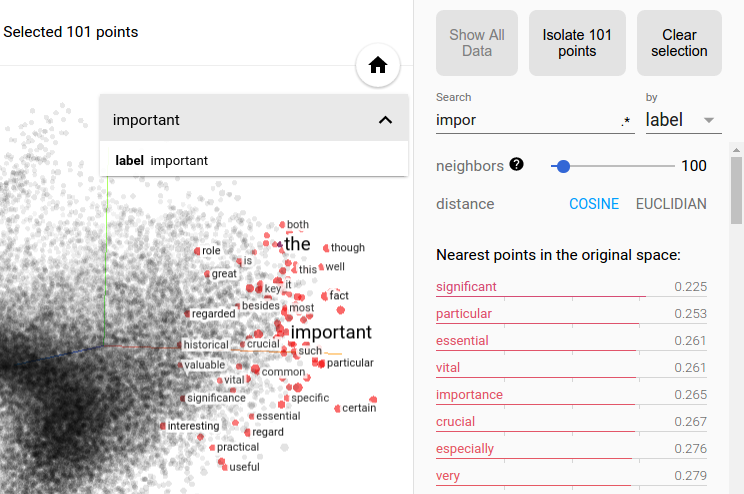
\includegraphics{embedding-nearest-points.png}
	\caption{important最相邻的embedding数据集}
\end{figure}
custom projection结合过滤会很有用,下面我们过滤和"politics"100个最相邻的点project他们在x轴上从好到坏向量表示,y轴水机。你可以看右边的我们有"ideas","science","perspective","journalism"左边有"crisis","violence"和"conflict"。
\begin{figure}
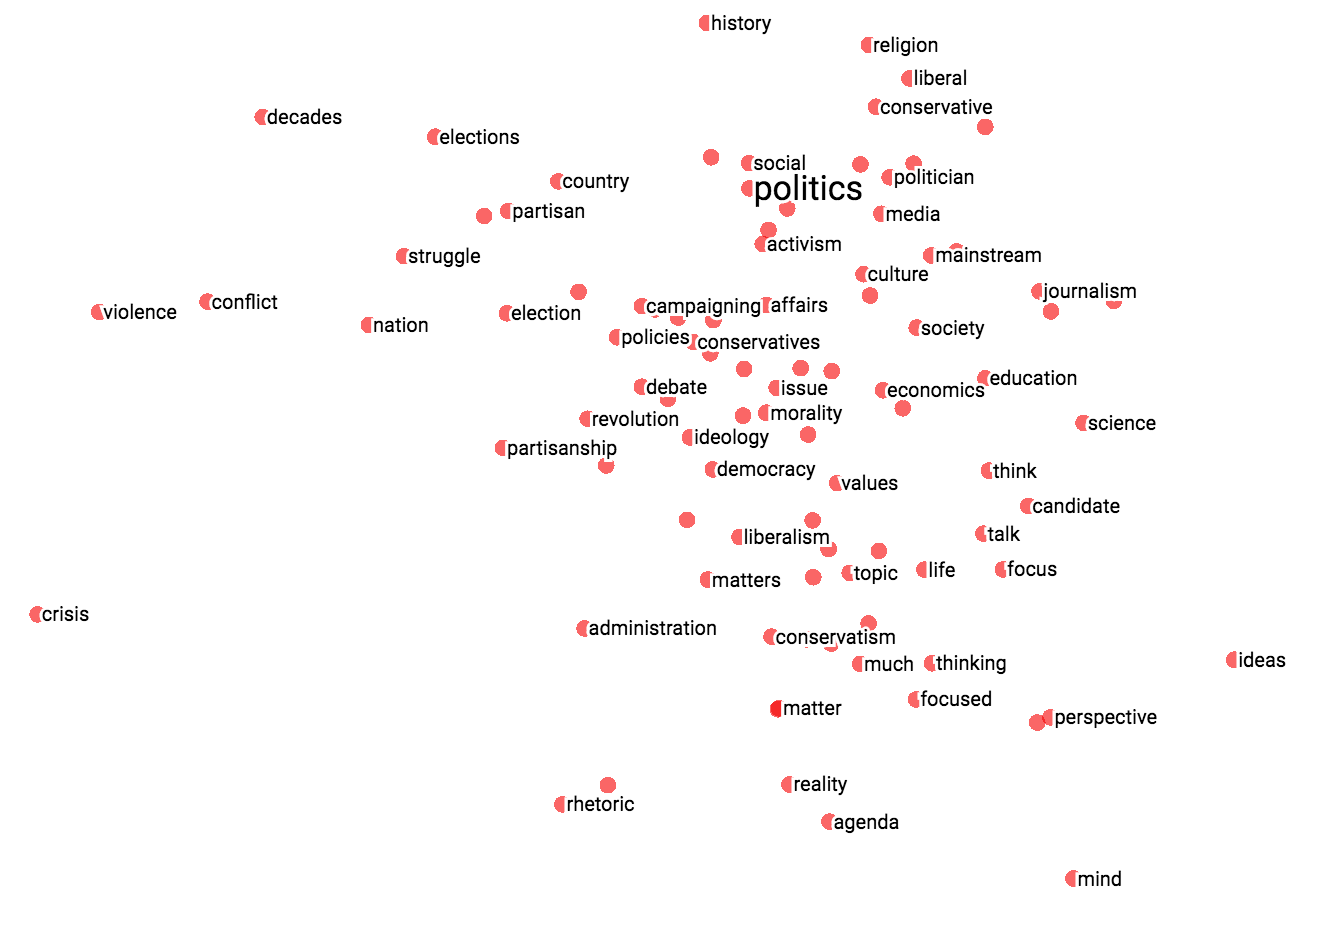
\includegraphics[scale=0.5]{embedding-custom-projection.png}
\end{figure}

\subsection{合作的特性}
为了分享你的发现你可以用右上角的bookmark面板保存当前状态(包括计算任何projection的坐标)为一个小文件。Projector可能被指定到一个或者更多文件,产生下面的面板,其他人可以通过标签序列查看。
\begin{figure}[H]
	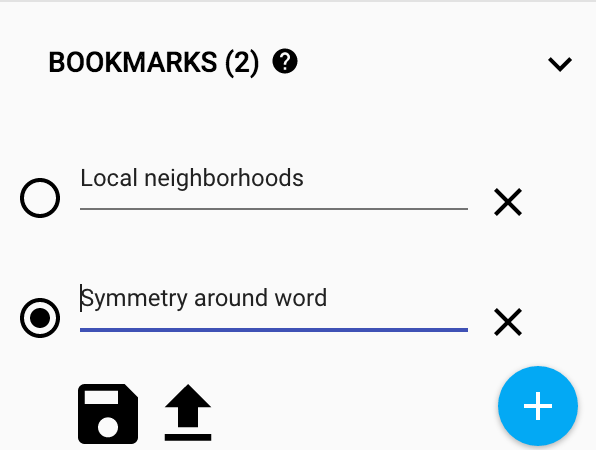
\includegraphics{embedding-bookmark.png}
\end{figure}
\subsection{简单的问答}
embedding是一个动作还是一个事物?两者都是,人们谈论向量空间的embedding word形成embedding(事物)。通常两个是一个从离散对象到向量映射embedding概念,创建应用映射是一个行为,但是映射是一个事物。

是高维还是低维embedding?300维的向量字词空间,例如当和上百万的字词空间相比是低维。但是数学上它是高维,显示了大量喝和人们直觉上的2位或者三维空间不一致的特性。

embedding和embedding layer是一样的吗?不是,一个embedding layer是神经网络的一部分,不是一个embedding是一个更常用的概念。

\begin{python}
#tensorflow 1.2.1
import tensorflow as tf
var = tf.Variable(0)
add_operation = tf.add(var,1)
update_operation = tf.assign(var,add_operation)
with tf.Session() as sess:
    sess.run(tf.global_variables_initializer())
    for _ in range(3):
        sess.run(update_operation)
        print(sess.run(var))
\end{python}
\subsection{placeholder}
\begin{python}
#tensorflow 1.2
import tensorflow as tf
x1 = tf.placeholder(dtype=tf.float32,shape=None)
y1 = tf.placeholder(dtype=tf.float32,shape=None)
z1 = x1+y1
x2 = tf.placeholder(dtype=tf.float32,shape=[2,1])
y2 = tf.placeholder(dtype=tf.float32,shape=[1,2])
z2 = tf.matmul(x2,y2)
with tf.Session() as sess:
    z1_value = sess.run(z1,feed_dict={x1:1,y1:2})
    z1_value,z2_value = sess.run([z1,z2],feed_dict={x1:1,y1:2,x2:[[2],[2]],y2:[[3,3]]})
    print(z1_value)
    print(z2_value)
\end{python}
\subsection{batch normalization}

\begin{itemize}
	\item[\S] 数据x为Tensor。
\item mean:为x的均值,也是一个Tensor。
\item var:为x的方差,也为一个Tensor。
\item offset:一个偏移,也是一个Tensor。
\item scale:缩放倍数,也是一个Tensor。
\item variable\_epsilon,一个不为0的浮点数。
\item name:操作的名字,可选。
\end{itemize}
batch normalization计算方式是:
\begin{gather}
x = (x-\bar{x})/\sqrt{Var(x)+variable_{epsilon}}\\
x = x\times scale+offset\\
\end{gather}
\begin{gather}
\text{均值}:\bar{x} = \frac{1}{m}\Sigma_{i=1}^{m}x_i\\
\text{方差}:\sigma^2 = \frac{1}{m}\Sigma_{i=1}^m(x_i-\bar{x})
\end{gather}
\section{常见的激活函数}
\subsection{relu}
relu函数在自变量x小于0时值全为0,在x大于0时,值和自变量相等。
\begin{python}
import tensorflow as tf 
import matplotlib.pyplot as plt 
x = tf.linspace(-10.,10.,100)
y = tf.nn.relu(x)
with tf.Session() as sess:
	[x,y] = sess.run([x,y])
plt.plot(x,y,'r',6,6,'bo')
plt.title('relu')
ax = plt.gca()
ax.annotate("",
            xy=(6, 6), xycoords='data',
            xytext=(6, 4.5), textcoords='data',
            arrowprops=dict(arrowstyle="->",
                            connectionstyle="arc3"),
            )
ax.annotate("",xy=(6,6),xycoords='data',
            xytext=(10, 6), textcoords='data',
            arrowprops=dict(arrowstyle="->",
                            connectionstyle="arc3"),
	  	   
)
ax.grid(True)
plt.xlabel('x')
plt.ylabel('relu(x)')
plt.savefig('relu.png',dpi = 600)
\end{python}
\subsection{relu6}
relu6函数和relu不同之处在于在x大于等于6的部分值保持为6。
\begin{python}
import tensorflow as tf 
import matplotlib.pyplot as plt 
x = tf.linspace(-10.,10.,100)
y = tf.nn.relu6(x)
with tf.Session() as sess:
	[x,y] = sess.run([x,y])
plt.plot(x,y,'r',6,6,'bo')
plt.title('relu6')
ax = plt.gca()
ax.annotate("",
            xy=(6, 6), xycoords='data',
            xytext=(6, 4.5), textcoords='data',
            arrowprops=dict(arrowstyle="->",
                            connectionstyle="arc3"),
            )
ax.grid(True)
plt.xlabel('x')
plt.ylabel('relu6(x)')
plt.savefig('relu6.png',dpi = 600)
\end{python}
\begin{figure}[H]
\centering
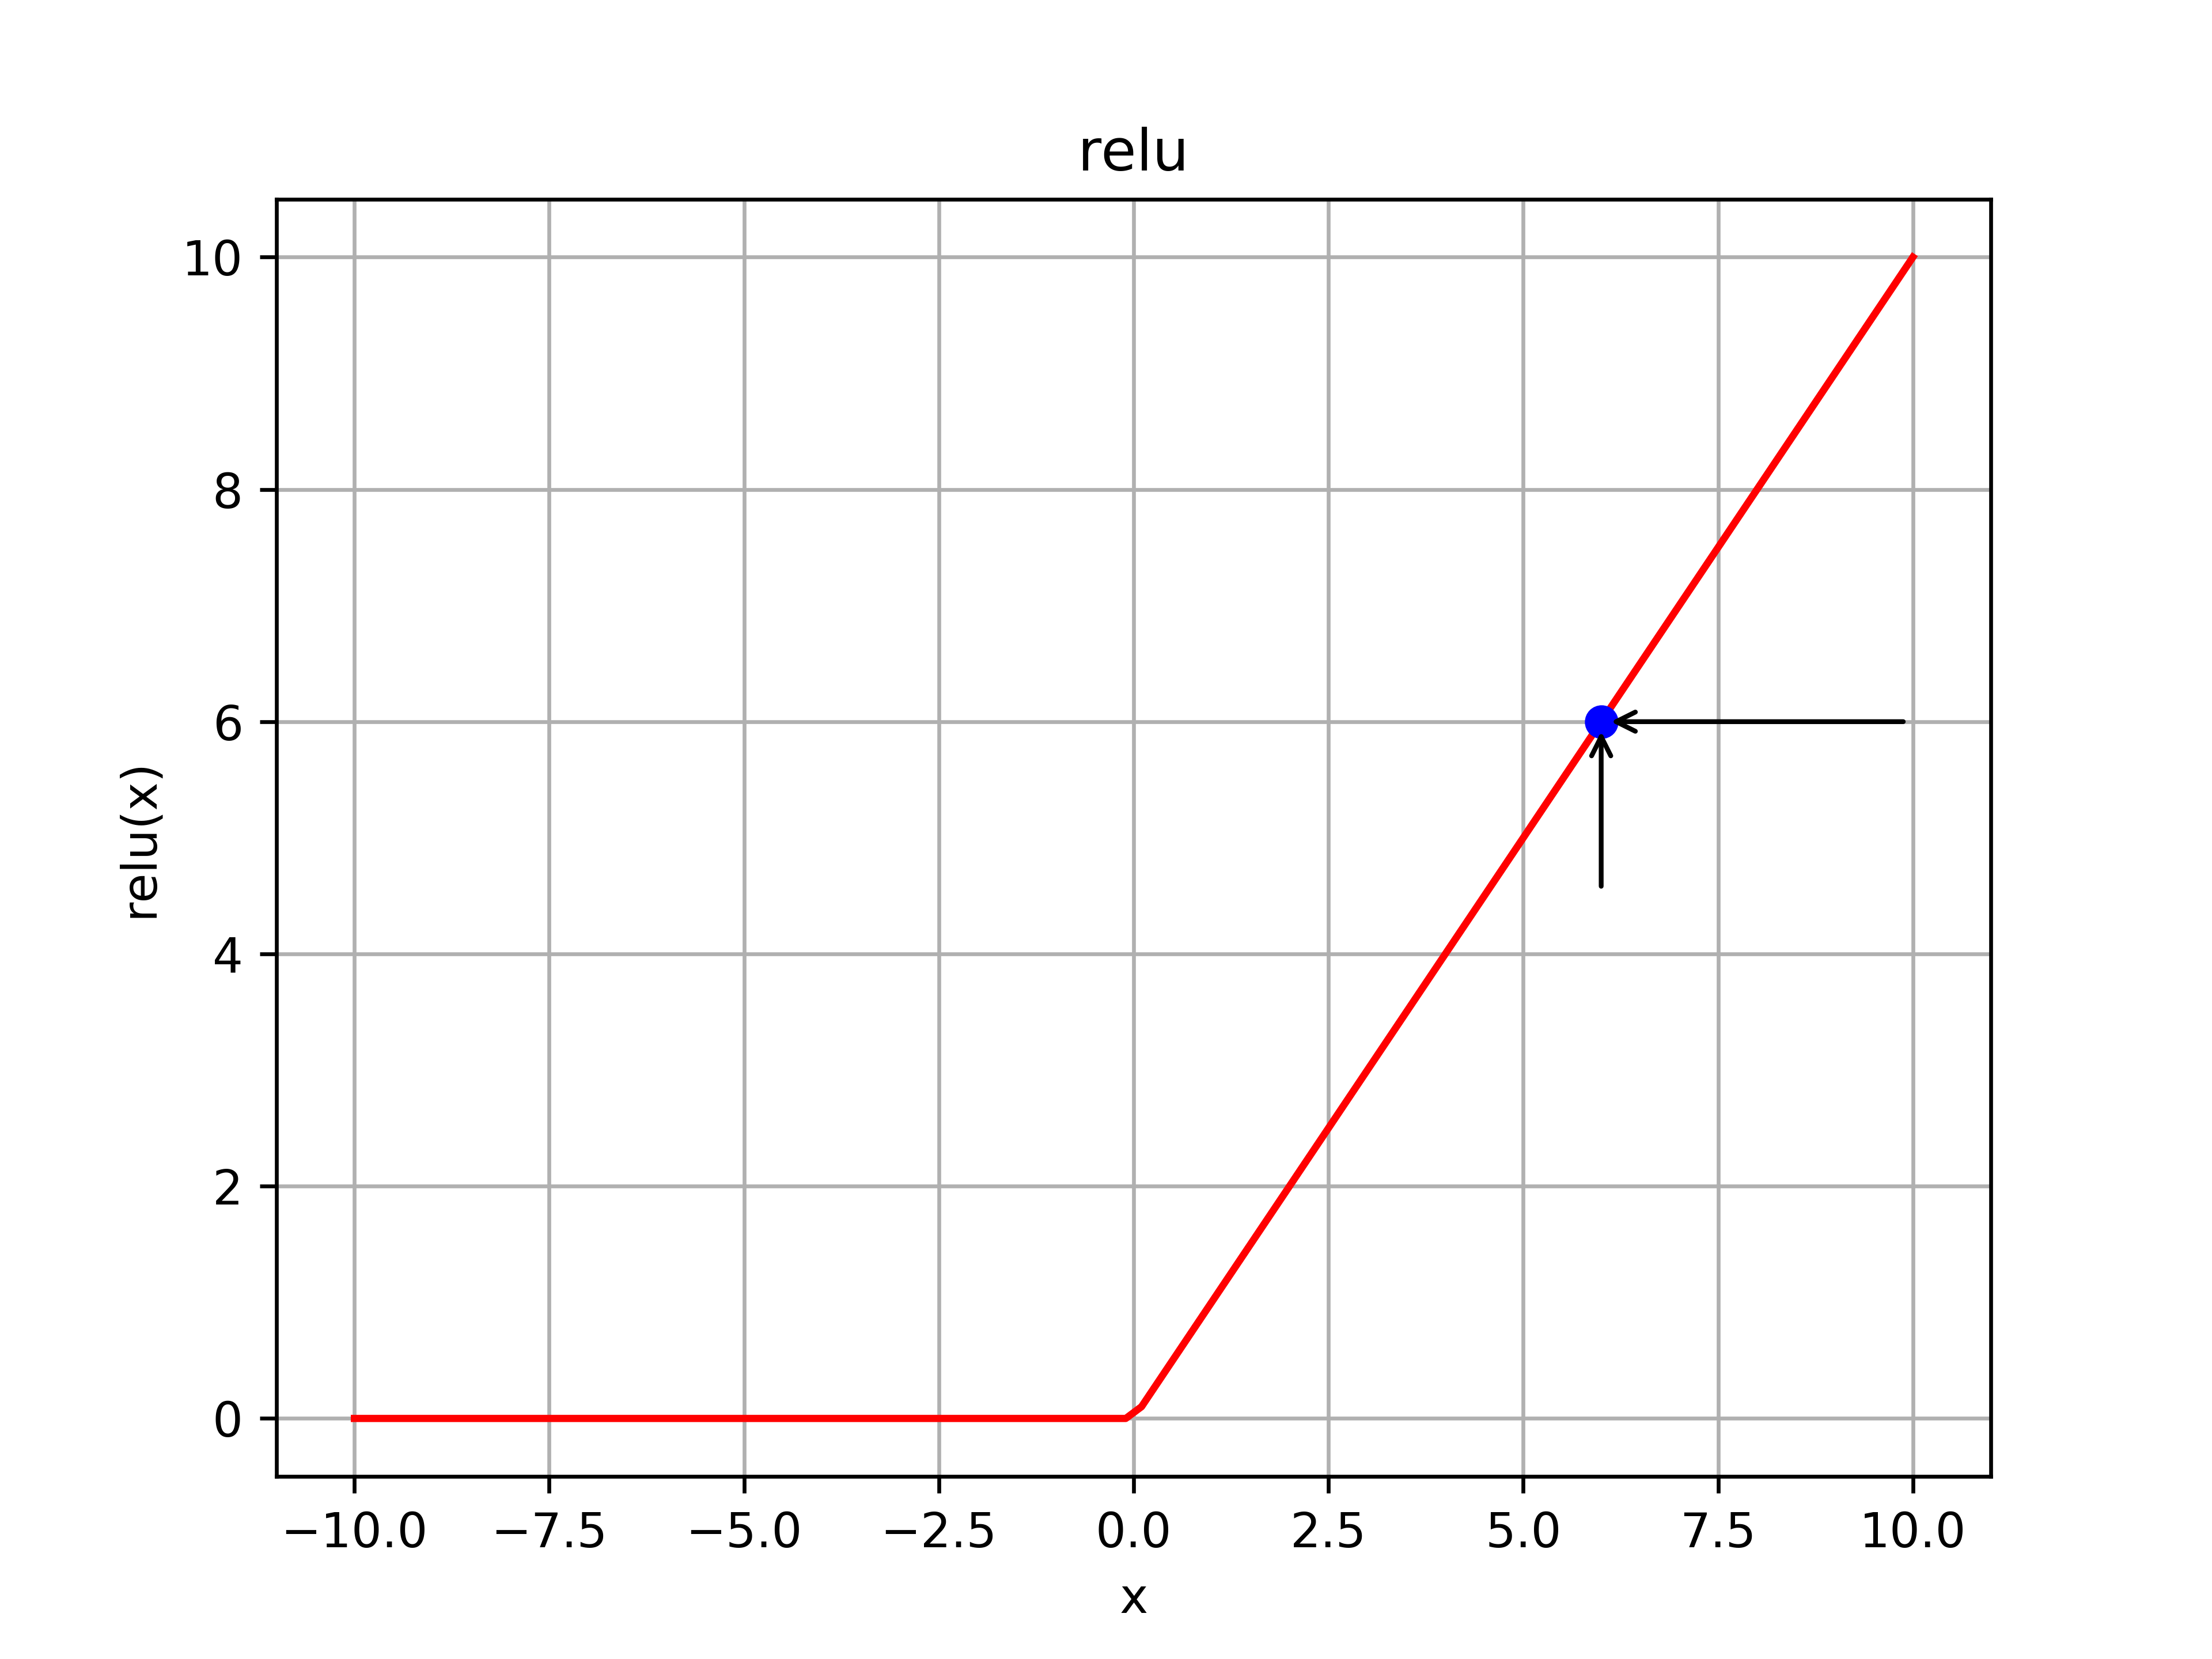
\includegraphics[scale=0.8]{./pic/chapter1/relu.png}
\caption{relu}
\end{figure}
\begin{figure}[H]
\centering
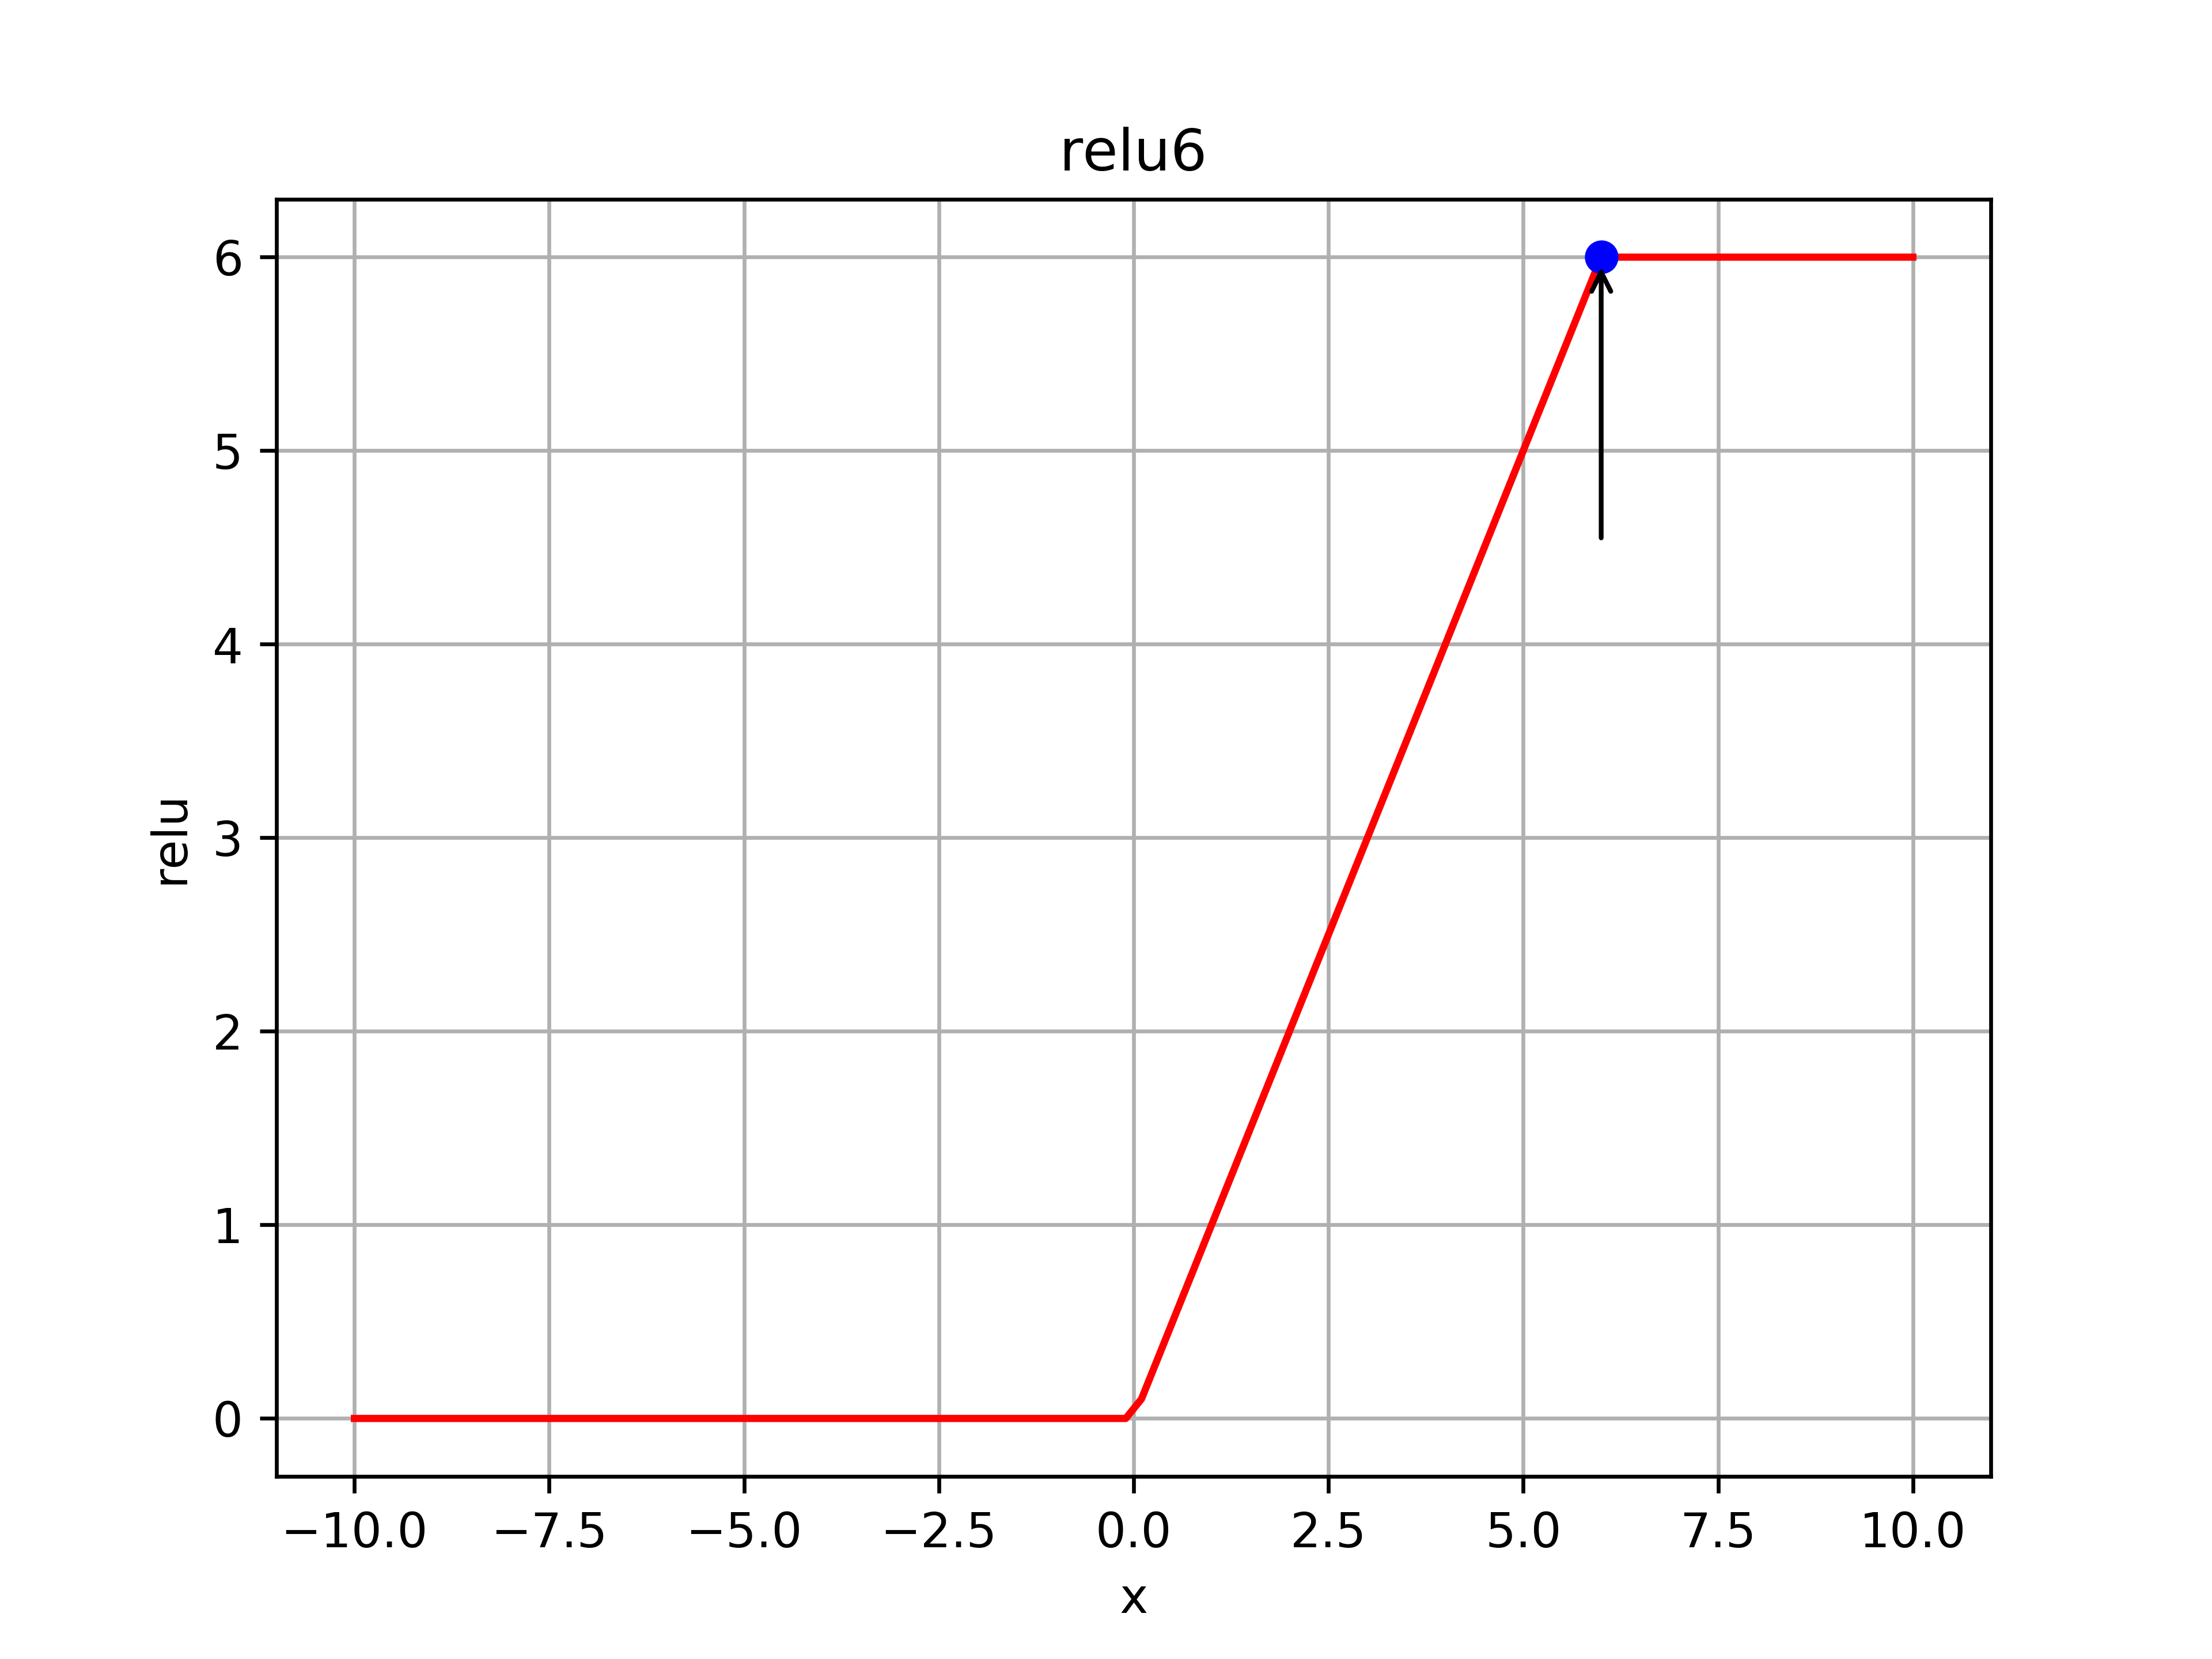
\includegraphics[scale=0.8]{./pic/chapter1/relu6.png}
\caption{relu6}
\end{figure}

\subsection{sigmoid}
\begin{python}
import tensorflow as tf 
import matplotlib.pyplot as plt 
import matplotlib.patches as mpatches
x = tf.linspace(-10.,10.,100)
y1 = tf.nn.sigmoid(x)
y2 = tf.nn.tanh(x)
red_patch = mpatches.Patch(color = 'red',label = 'sigmoid')
blue_patch = mpatches.Patch(color = 'blue',label = 'tanh')
with tf.Session() as sess:
	[x,y1,y2] = sess.run([x,y1,y2])
plt.plot(x,y1,'r',x,y2,'b')
ax = plt.gca()
ax.annotate(r"$tanh(x) = \frac{1-^{-2x}}{1+e^{-x}}$",
	   xy=(0,0),xycoords="data",
	   xytext=(1,0),textcoords="data",
	   arrowprops=dict(arrowstyle="->",
	   connectionstyle="arc3"),
)
ax.annotate(r"$sigmoid(x) = \frac{1}{1+e^{-x}}$",
	   xy=(0,0.5),xycoords="data",
	   xytext=(1,0.5),textcoords="data",
	   arrowprops=dict(arrowstyle="->",
	   connectionstyle="arc3"),
)
plt.xlabel('x')
plt.grid(True)
plt.legend(handles = [red\_patch,blue\_patch])
plt.savefig('activate.png',dpi=600)
\end{python}
\begin{figure}[H]
\centering
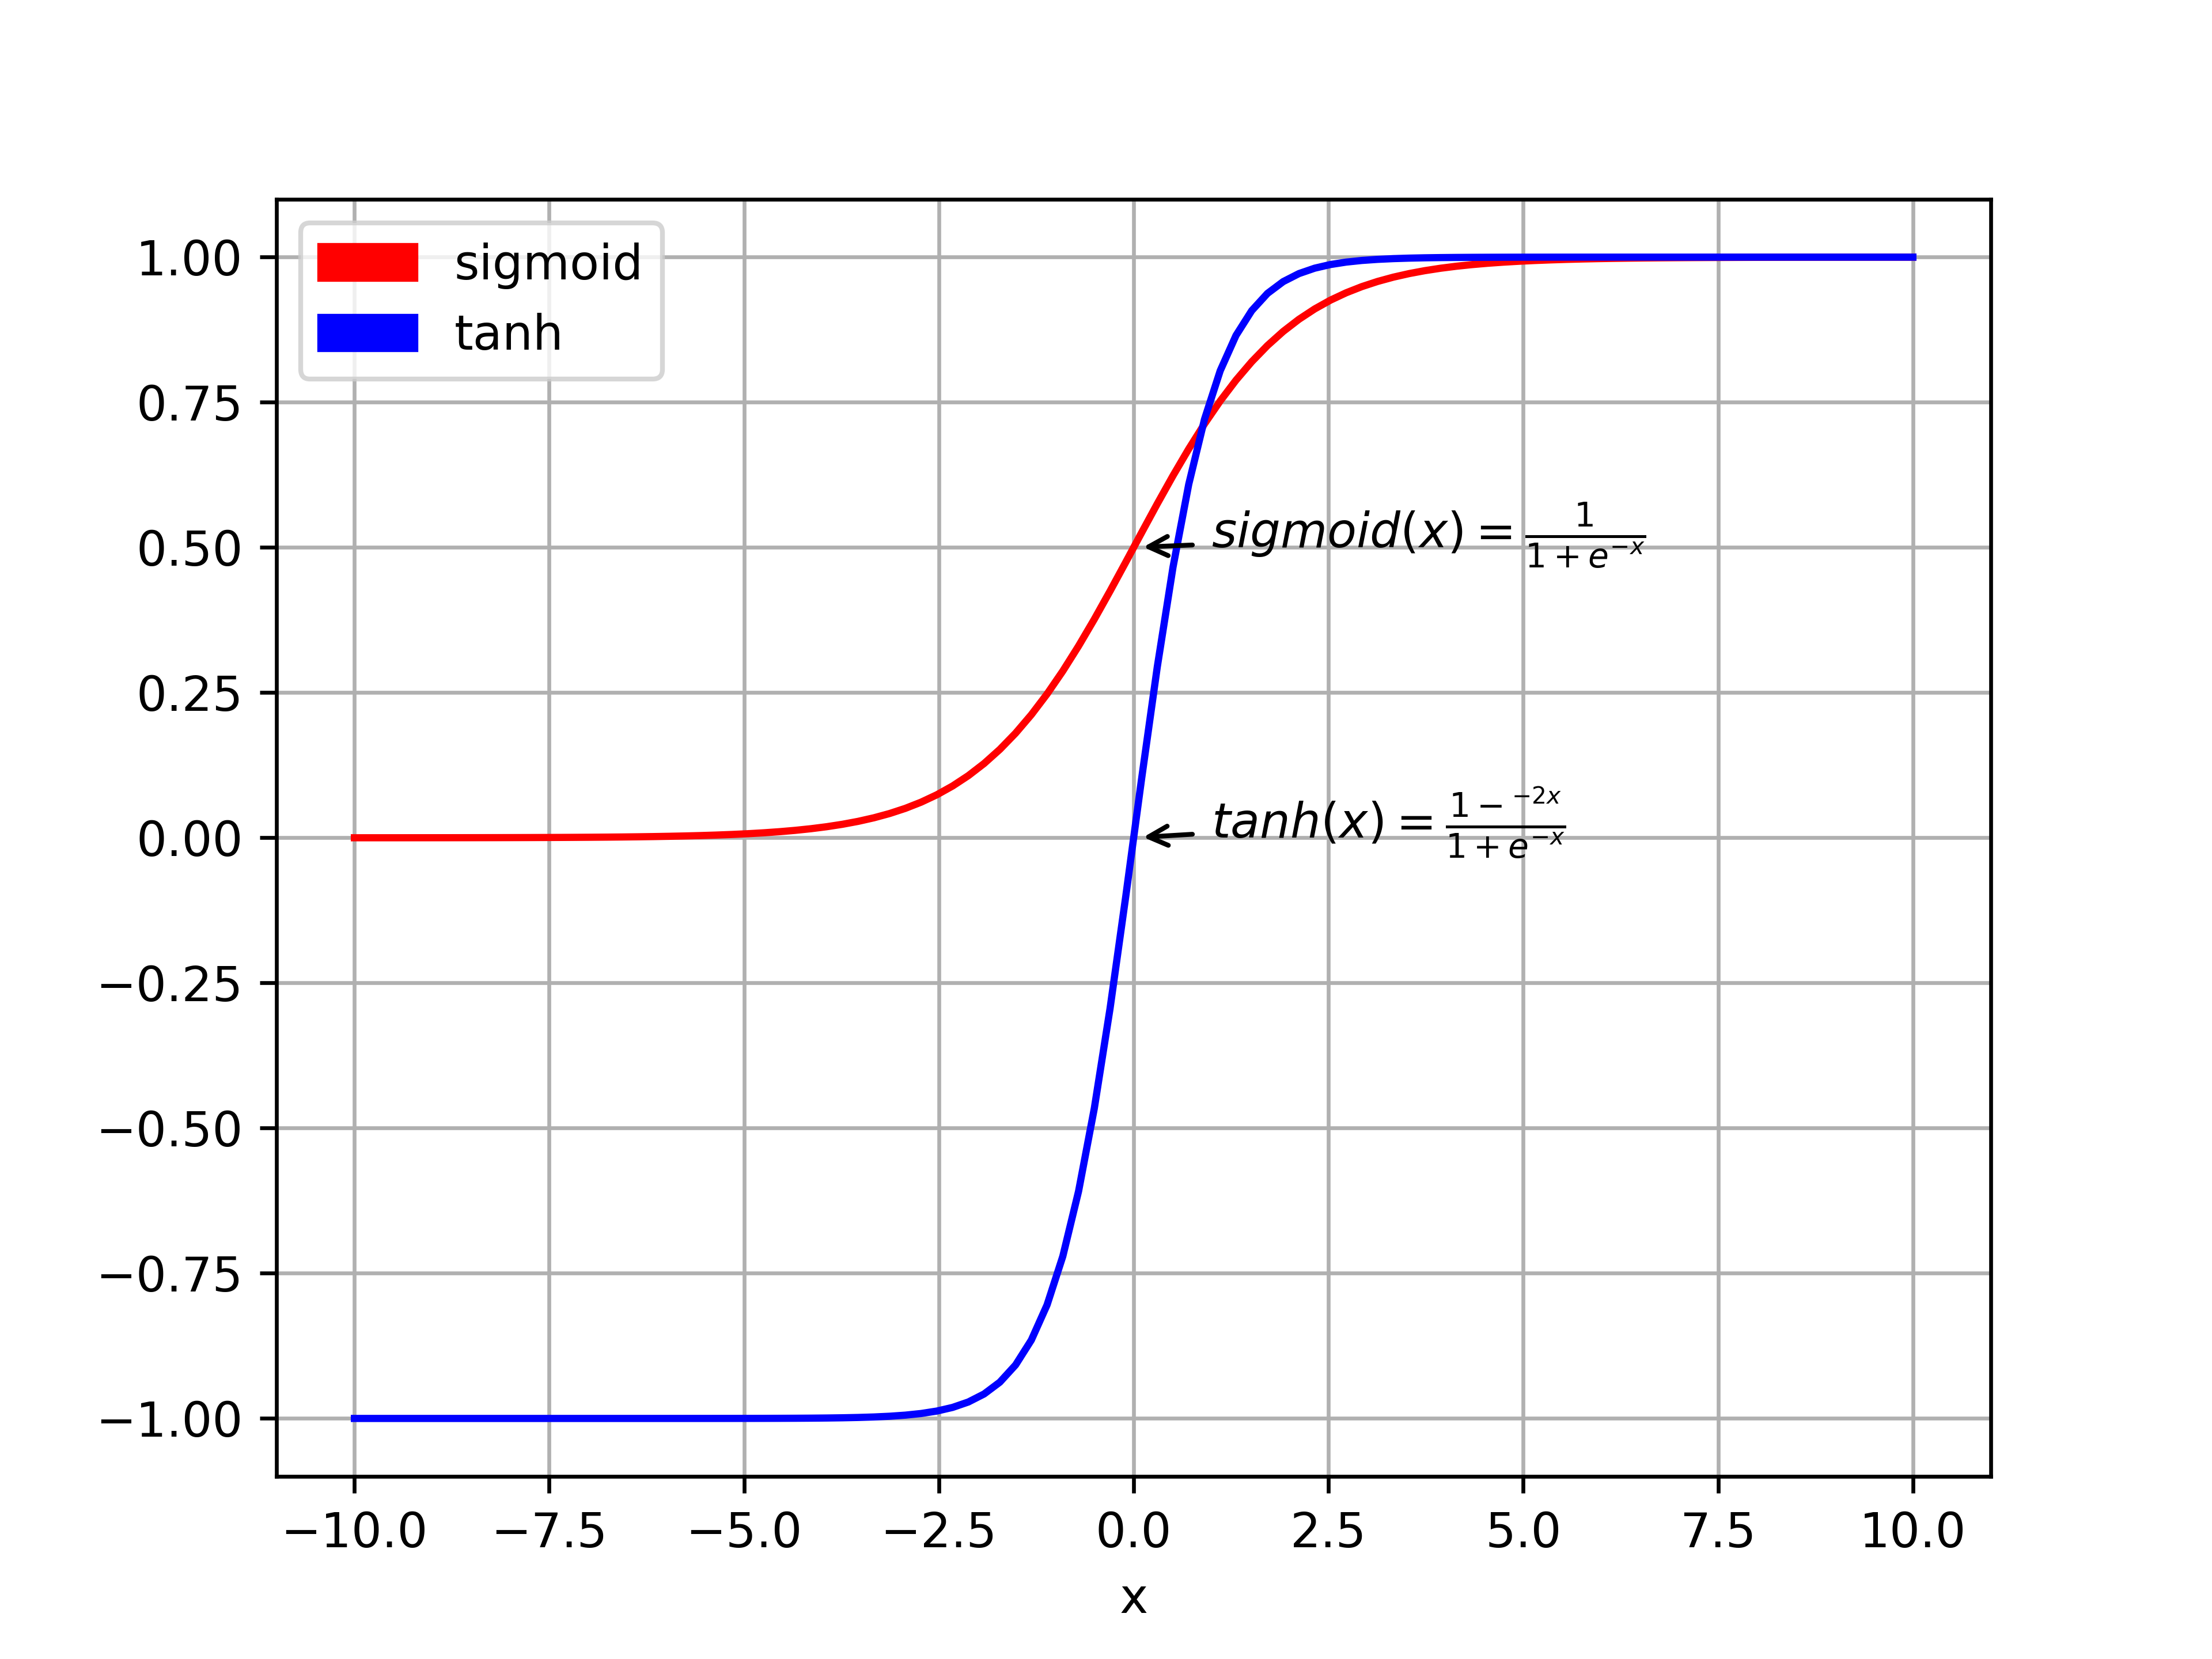
\includegraphics[scale=0.8]{./pic/chapter1/activate_fun.png}
\caption{activate\_fun}
\end{figure}
\subsection{relu和softplus}
\begin{python}
import tensorflow as tf 
import matplotlib.pyplot as plt 
import matplotlib.patches as mpatches
x = tf.linspace(-10.,10.,100)
y2 = tf.nn.softplus(x)
y3 = tf.nn.relu(x)
blue_patch = mpatches.Patch(color = 'blue',label = 'softplus')
yellow_patch = mpatches.Patch(color = 'yellow',label = 'relu')
with tf.Session() as sess:
	[x,y2,y3] = sess.run([x,y2,y3])
plt.plot(x,y2,'b',x,y3,'y')
ax = plt.gca()
plt.xlabel('x')
ax.annotate(r"$softplus(x)=log(1+e^x)$",
	   xy=(0,0),xycoords="data",
	   xytext=(1,0),textcoords="data",
	   arrowprops=dict(arrowstyle="->",
	   connectionstyle="arc3"),
)
ax.annotate(r"$relu(x)=max(x,0)$",
	   xy=(0,0.5),xycoords="data",
	   xytext=(1,0.5),textcoords="data",
	   arrowprops=dict(arrowstyle="->",
	   connectionstyle="arc3"),
)

plt.grid(True)
plt.legend(handles = [blue_patch,yellow_patch])
plt.savefig('relu_softplus.png',dpi=600)
\end{python}
\begin{figure}[H]
\centering
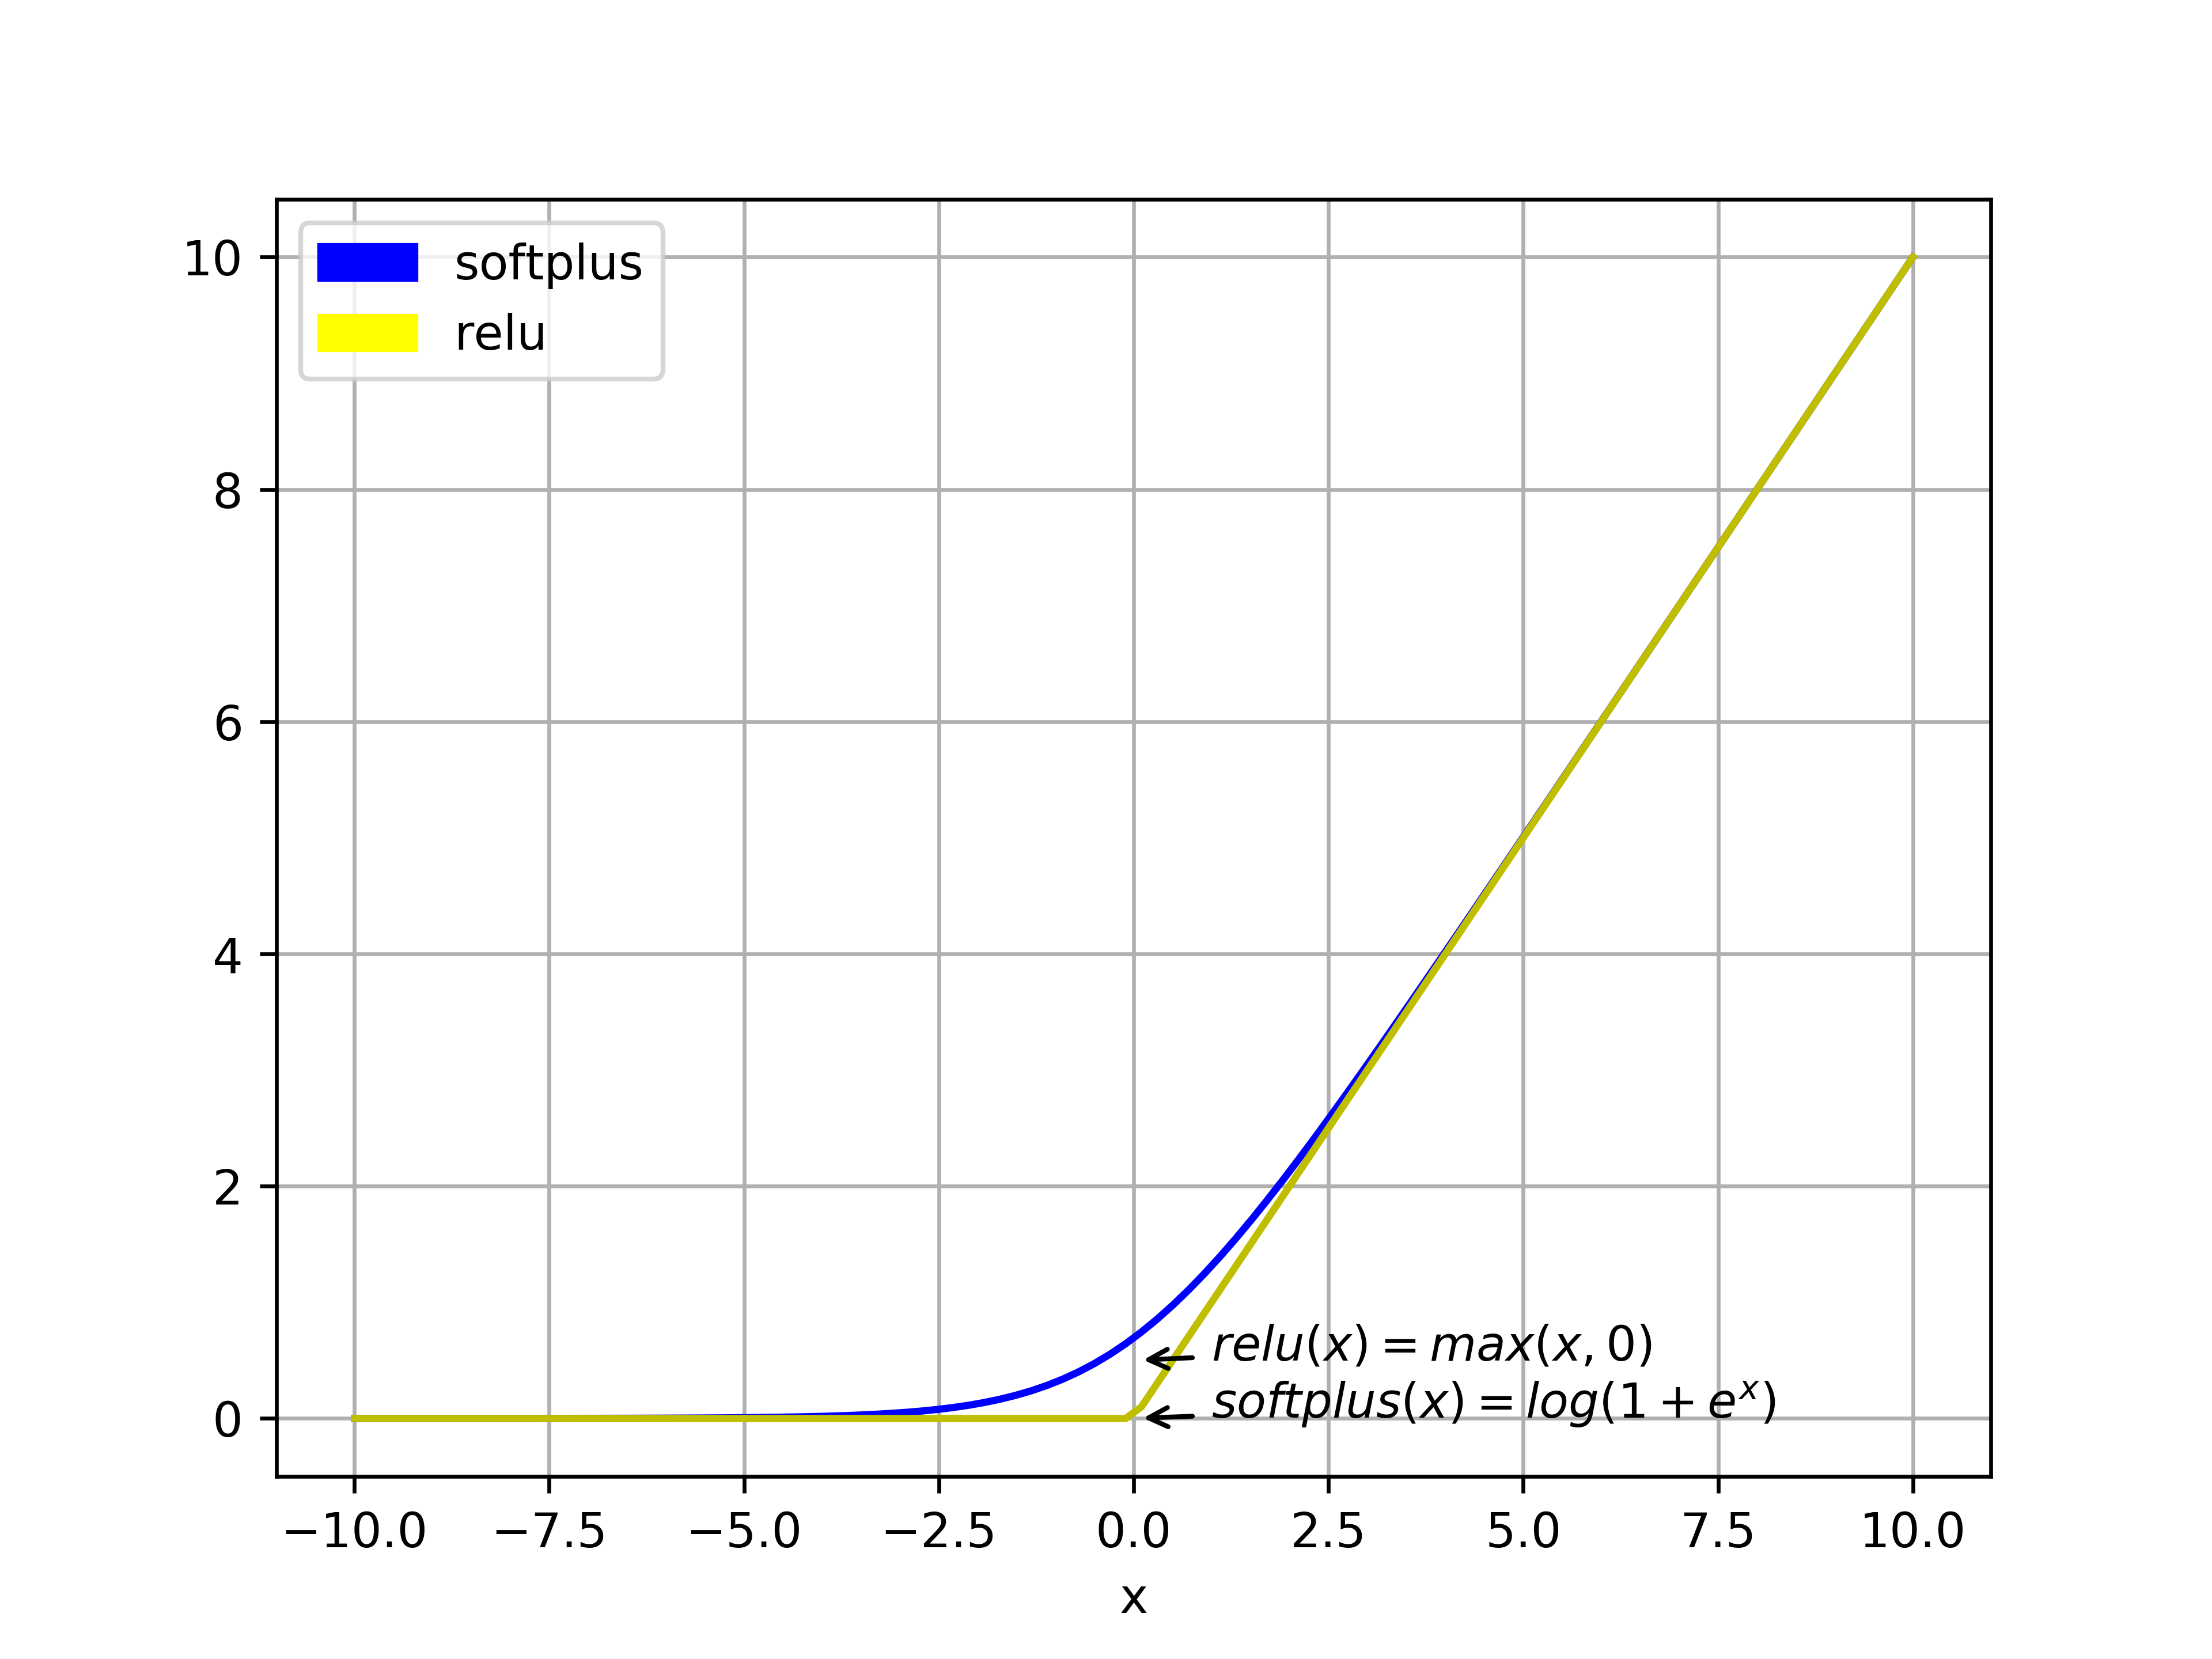
\includegraphics[scale=0.8]{./pic/chapter1/relu_softplus.png}
\end{figure}
\subsection{dropout}
将神经元以概率keep\_prob绝对是否被抑制。如果被抑制该神经元的输出为0如果不被抑制,该神经元的输出将被放大到原来的1/keep\_prop。
默认情况下,每个神经元是否被抑制是相互独立的。但是是否被抑制也可以通过noise\_shape来调节。当noise\_shape[i]=shape(x)[i]时,x中的元素相互独立。如果shape(x)=[k,1,1,n],那么每个批通道都是相互独立的,但是每行每列的数据都是关联的,也就是说要么都为0,要么还是原来的值。
\begin{python}
import tensorflow as tf
a = tf.constant([[-1.,2.,3.,4.]])
with tf.Session() as sess:
    b = tf.nn.dropout(a,0.5,noise_shape=[1,4])
    print(sess.run(b))
    c = tf.nn.dropout(a,0.5,noise_shape=[1,1])
    print(sess.run(c))
\end{python}
[[-2.  0.  0.  8.]]\newline
[[-0.  0.  0.  0.]]\newline
当输入数据特征相差明显时,用tanh效果会很好,但在循环过程中会不断扩大特征效果并显示出来。当特征相差不明显时,sigmoid效果比较好。同时,用sigmoid和tanh作为激活函数时,需要对输入进行规范化,否则激活厚的值全部进入平坦区,隐藏层的输出会趋同,丧失原来的特征表达,而relu会好很多,优势可以不需要输入规范化来避免上述情况。因此,现在大部分卷积神经网络都采用relu作为激活函数。
\section{CNN常用函数}
\subsection{卷积函数}
tf.nn.conv2d(input,filter,padding,stride=None,diation\_rate=Nonei每name = None,data\_format=None)\newline
\begin{itemize}
\item input:一个tensor,数据类型必须是float32,或者是float64
\item filter:一个tensor,数据类型必须和input相同。
\item strides:一个长度为4的一组证书类型数组,每一维对应input中每一维对应移动的步数,strides[1]对应input[1]移动的步数。
\item padding:有两个可选参数'VALID'(输入数据维度和输出数据维度不同)和'SAME'(输入数据维度和输出数据维度相同)
\item use\_cudnn\_on\_gpu:一个可选的布尔值,默认情况下时True。
\item name:可选,操作的一个名字。
\end{itemize}
\begin{python}
import tensorflow as tf
input_data = tf.Variable(tf.random_normal(shape = [10,9,9,3],mean=0,stddev=1),dtype = tf.float32)
kernel = tf.Variable(tf.random_normal(shape = [2,2,3,2],mean = 0,stddev=1,dtype=tf.float32))

y = tf.nn.conv2d(input_data,kernel,strides=[1,1,1,1],padding='SAME')
init = tf.global_variables_initializer()
with tf.Session() as sess:
    sess.run(init)
    print(sess.run(y).shape)
\end{python}
输出形状为[10,9,9,2]。
\subsection{常见的分类函数}
tf.nn.sigmoid\_cross\_entropy\_with\_logits(logits,targets,name=None)
\begin{itemize}
	\item logits:[batch\_size,num\_classes]
	\item targets:[batch\_size,size]
	\item 输出:loss[batch\_size,num\_classes]
\end{itemize}
最后已成不需要进行sigmoid操作。\par
tf.nn.softmax(logits,dim=-1,name=None):计算Softmax
\[softmax = \frac{x^{logits}}{reduce\_sum(e^{logits},dim)}\]
tf.nn.log\_softmax(logits,dim=-1,name = None)计算log softmax
\[logsoftmax = logits-log(reduce\_softmax(exp(logits),dim))\]
tf.nn.softmax\_cross\_entropy\_with\_logits(\_setinel=None,labels=None,logits=None,dim=-1,name=None)
输出loss:[batch\_size]保存的时batch中每个样本的交叉熵。
tf.nn.sparse\_softmax\_cross\_entropy\_with\_logic(logits,labels,name=None)
\begin{itemize}
	\item logits:神经网络最后一层的结果。
	\item 输入logits:[batch\_size,num\_classes],labels:[batch\_size],必须在[0,num\_classes]
	\item loss[batch],保存的是batch每个样本的交叉熵。
\end{itemize}
\section{优化方法}
\begin{itemize}
	\item tf.train.GradientDescentOptimizer
	\item tf.train.AdadeltaOptimizer
	\item tf.train.AdagradDAOptimizer
	\item tf.train.AdagradOptimizer
	\item tf.train.MomentumOptimizer
	\item tf.train.AdamOptimizer
	\item tf.train.FtrlOptimizer
	\item tf.train.RMSPropOptimizer
\end{itemize}
\subsection{BGD}
BGD(batch gradient descent)批量梯度下降。这种方法是利用现有的参数对训练集中的每一个输入生成一个估计输出$y_i$,然后跟实际的输出$y_i$比较,统计所有的误差,求平均后的到平均误差作为更新参数的依据。啊他的迭代过程是:
\begin{enumerate}
	\item 提取训练集集中所有内容$\{x_1,\ldots,x_n\}$,以及相关的输出$y_i$;
	\item 计算梯度和误差并更新参数。
\end{enumerate}
这种方法的优点是:使用所有数据计算,都保证收敛,并且不需要减少学习率。缺点是每一步需要使用所有的训练数据,随着训练的进行,速度会变慢。那么如果将训练数据拆分成一个个batch,每次抽取一个batch数据更新参数,是不是能加速训练?这就是SGD。
\subsection{SGD}
SGD(stochastic gradient descent):随机梯度下降。这种方法的主要思想是将数据集拆分成一个个的batch,随机抽取一个batch计算并更新参数,所以也称为MBGD(minibatch gradient descent)\
SGD在每次迭代计算mini-batch的梯度,然后对参数进行更新。和BGD相比,SGD在训练数据集很大时也能以较快的速度收敛,但是它有两个缺点:
\begin{enumerate}
\item 需要手动调整学习率,此外选择合适的学习率比较困难。尤其在训练时,我们常常想对常出现的特征更快速的更新,对不常出现的特征更新速度慢些,而SGD更新参数时对所有参数采用一样的学习率,因此无法满足要求。
\item SGD:容易收敛到局部最优。
\end{enumerate}
\subsection{momentum}
Momentum是模拟物理学中的动量概念,更新时在一定程度上保留之前的更新方向,利用当前批次再次微调本次更新参数,因此引入了一个新的变量v,作为前几次梯度的累加。因此,momentum能够更新学习率,在下降初期,前后梯度方向一致时能加速学习:在下降的中后期,在局部最小值附近来回振荡,能够抑制振荡加快收敛。
\subsection{Nesterov Momentum}
标准的Monentum法首先计算一个梯度,然后在加速更新梯度的方向进行一个大的跳跃Nesterov首先在原来加速的梯度方向进行一个大的跳跃,然后在改为值设置计算梯度值,然后用这个梯度值修正最终的更新方向。
\subsection{Adagrad}
Adagrade能够自适应的为各个参数分配不同的学习率,能够控制每个维度的梯度方向,这种方法的优点是能实现学习率的自动更改,如果本次更新时梯度大,学习率就衰减得快,如果这次更新时梯度小,学习率衰减得就慢些。
\subsection{RMSprop}
和Momentum类似,通过引入衰减系数使得每个回合都衰减一定比例。在实践中,对循环神经网络效果很好。
\subsection{Adam}
名称来自自适应矩阵(adaptive moment estimation).Adam根据损失函数针对每个参数的一阶矩,二阶矩估计动态调整每个参数的学习率。
\begin{python}
import numpy as np
import tensorflow as tf
import matplotlib.pyplot as plt
tf.set_random_seed(0)
np.random.seed(0)
LR = 0.01
BATCH_SIZE = 32
x = np.linspace(-1,1,100).reshape(-1,1)
noise = np.random.normal(0,0.1,size=x.shape)
y = np.power(x,2)+noise
class Net:
    def __init__(self,opt,**kwargs):
        self.x = tf.placeholder(tf.float32,[None,1])
        self.y = tf.placeholder(tf.float32,[None,1])
        l = tf.layers.dense(self.x,20,tf.nn.relu)
        out = tf.layers.dense(l,1)
        self.loss = tf.losses.mean_squared_error(self.y,out)
        self.train = opt(LR,**kwargs).minimize(self.loss)
net_SGD = Net(tf.train.GradientDescentOptimizer)
net_momentum = Net(tf.train.MomentumOptimizer,momentum=0.9)
net_RMSprop = Net(tf.train.RMSPropOptimizer)
net_Adam = Net(tf.train.AdamOptimizer)
nets = [net_SGD,net_momentum,net_RMSprop,net_Adam]
sess = tf.Session()
sess.run(tf.global_variables_initializer())
losses_his = [[],[],[]]
for step in range(300):
    index = np.random.randint(0,x.shape[0],BATCH_SIZE)
    b_x = x[index]
    b_y = y[index]
    for net,l_his in zip(nets,losses_his):
        _,l = sess.run([net.train,net.loss],{net.x:b_x,net.y:b_y})
        l_his.append(l)
labels = ['SGD','Momentum','RMSprop','Adam']
for i,l_his in enumerate(losses_his):
    plt.plot(l_his,label=labels[i])
plt.legend(loc='best')
plt.xlabel('Step')
plt.ylabel('Loss')
plt.ylim(0,0.2)
plt.savefig('Opt.png',dpi=600)
\end{python}
\begin{figure}[H]
	\centering
	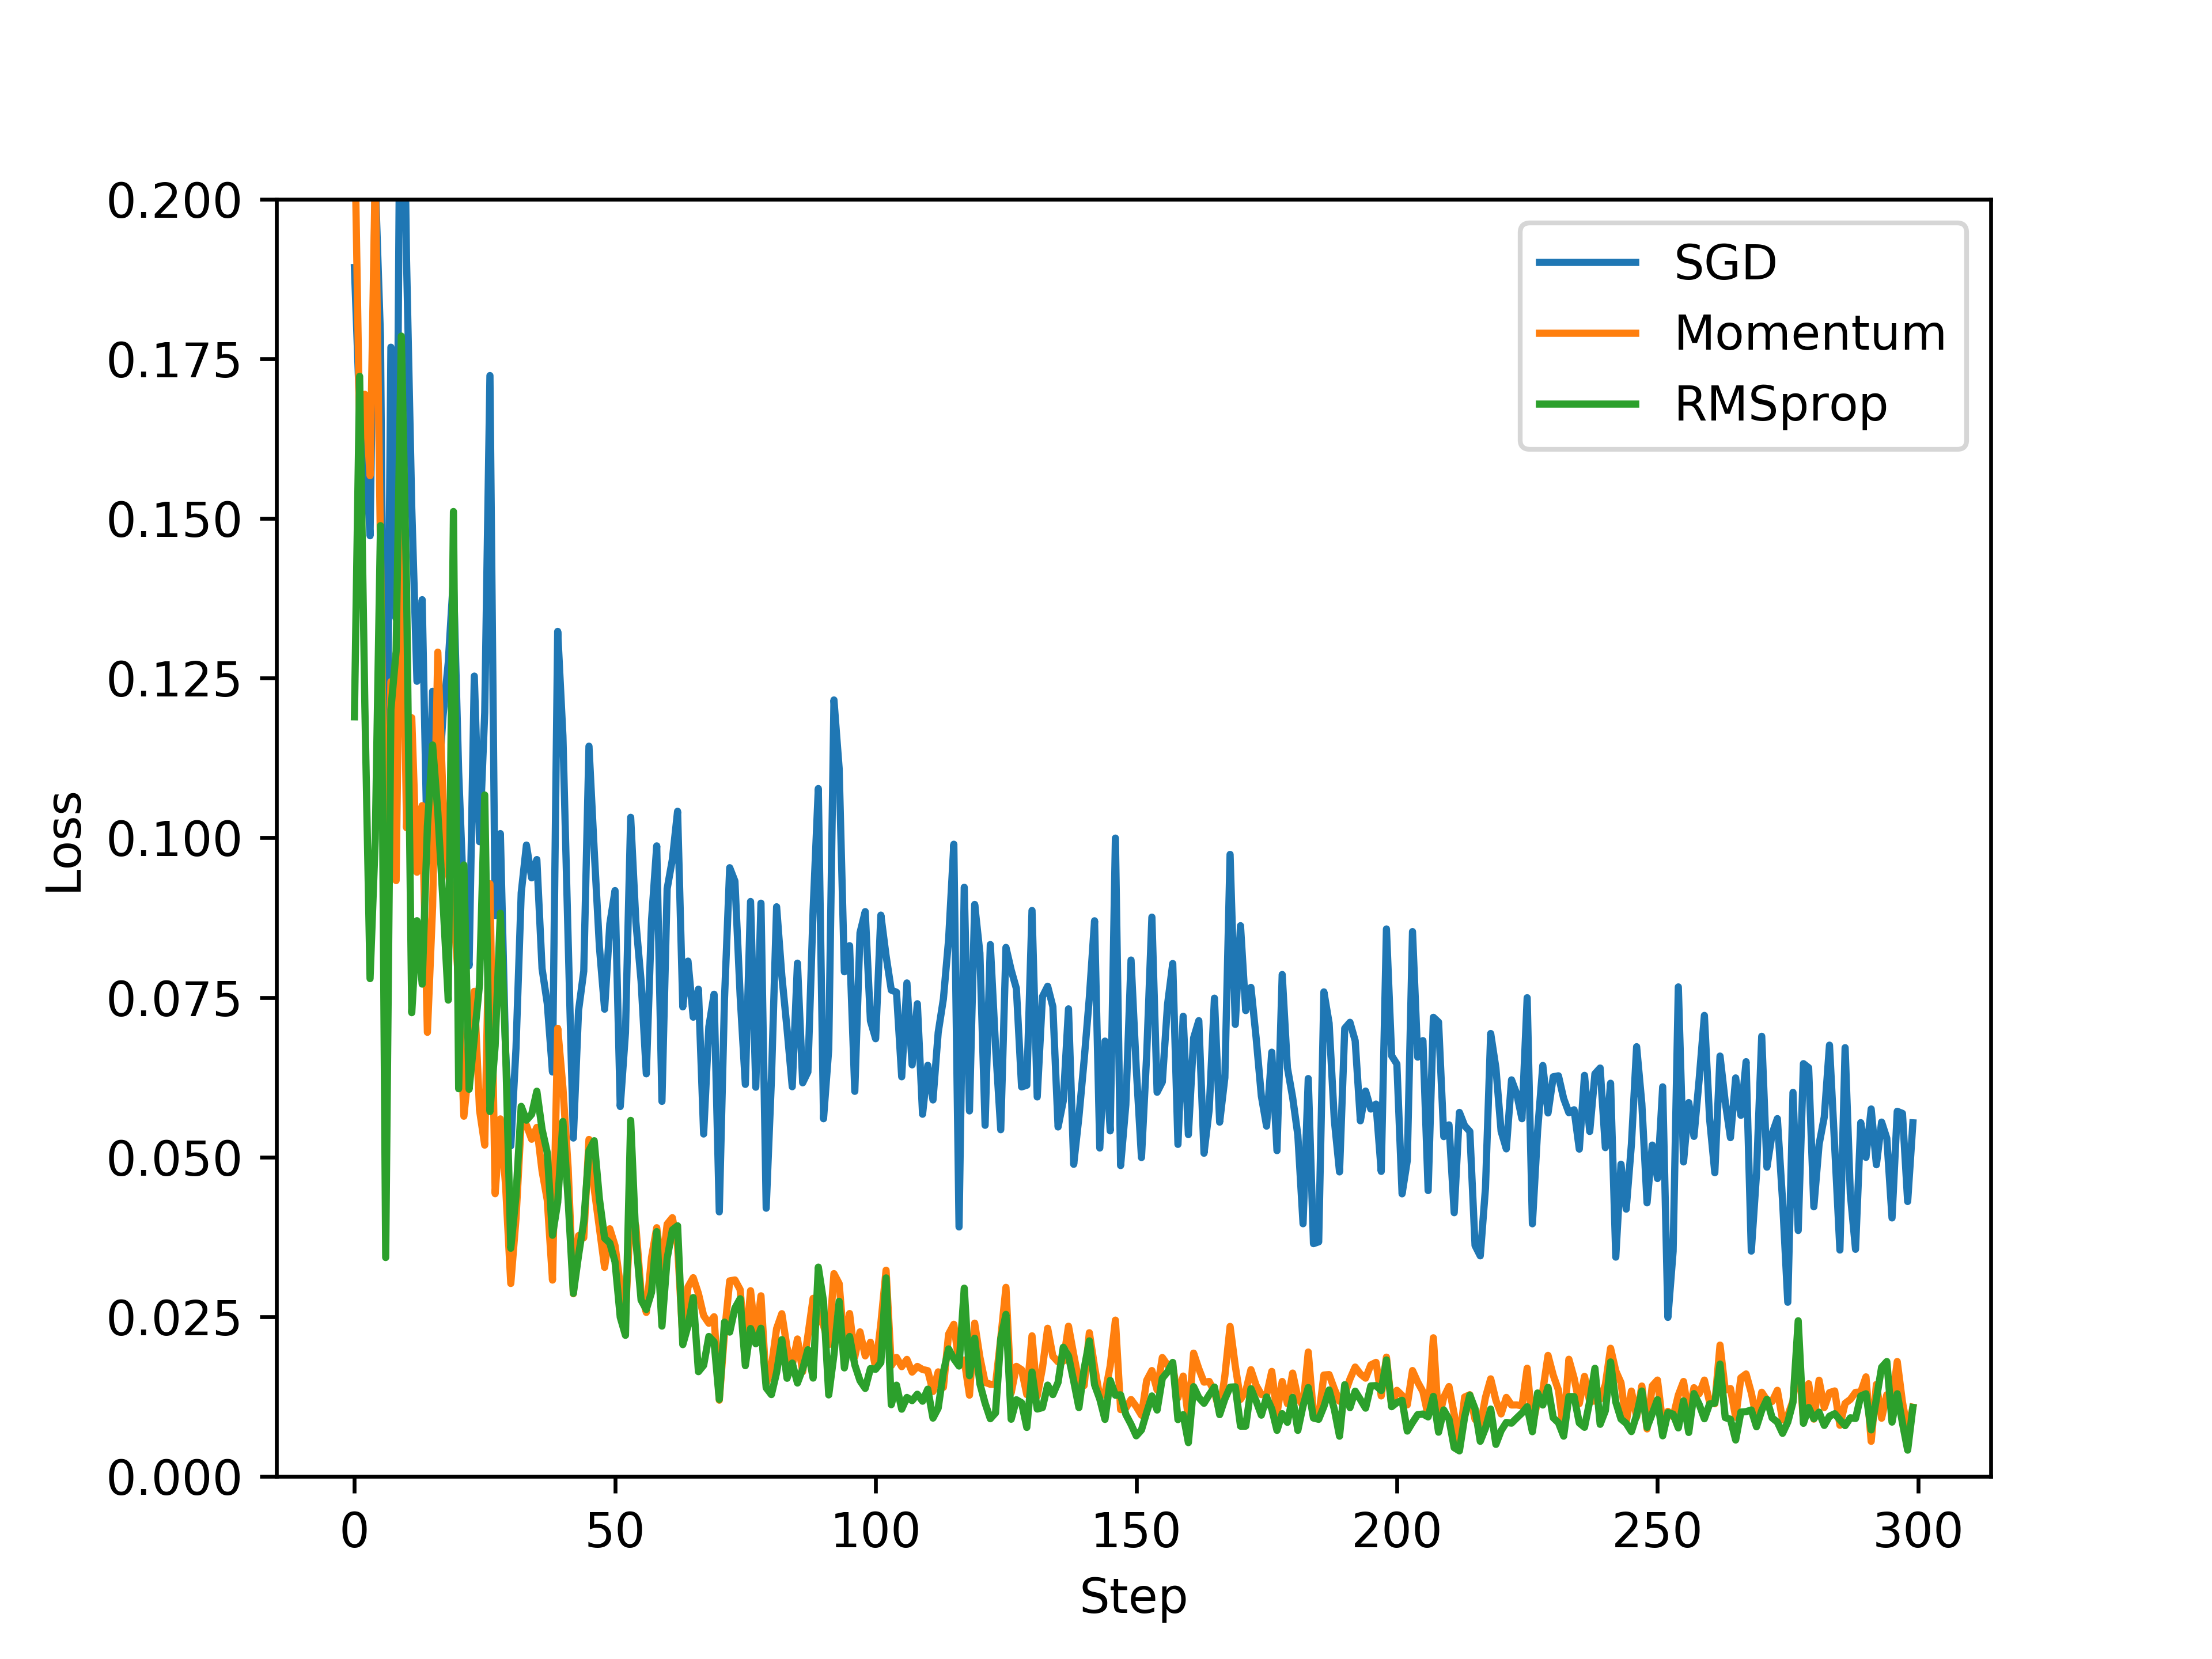
\includegraphics[scale=0.6]{./pic/chapter1/Opt.png}
\end{figure}
\subsection{构造简单的神经网络拟合数据}
原始数据为$y=x^2$的基础上添加随机噪声。原始数据的散点图如下
\begin{center}
\begin{figure}[H]
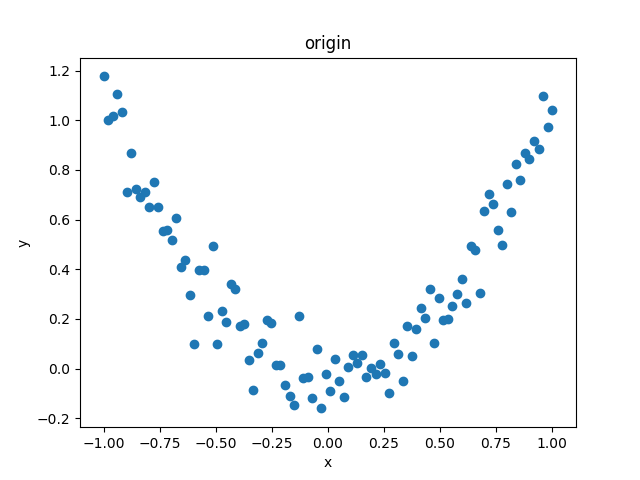
\includegraphics[scale=0.6]{./pic/chapter1/origin.png}
\end{figure}
\end{center}
\begin{python}
#tensorflow 1.2.1
import tensorflow as tf
import matplotlib.pyplot as plt
import numpy as np
tf.set_random_seed(0)
np.random.seed(0)
#生成数据
step = 100
x = np.linspace(-1,1,step).reshape(-1,1)
noise = np.random.normal(0,0.1,size=x.shape)
y = np.power(x,2)+noise

tf_x = tf.placeholder(tf.float32,x.shape)
tf_y = tf.placeholder(tf.float32,x.shape)
l1 =  tf.layers.dense(tf_x,10,tf.nn.relu)
output = tf.layers.dense(l1,1)

loss = tf.losses.mean_squared_error(tf_y,output)
optimizer = tf.train.GradientDescentOptimizer(learning_rate=0.5)
train_op = optimizer.minimize(loss)

sess = tf.Session()
sess.run(tf.global_variables_initializer())
plt.ion()
for step in range(100):
    _,l,pred = sess.run([train_op,loss,output],{tf_x:x,tf_y:y})
    if step%5==0:
        plt.cla()
        plt.scatter(x,y)
        plt.title(r'$y=x^2+noise$')
        plt.plot(x,pred,'r-',lw=2)
        plt.text(0,0.8,'Loss=%.4f'%l,fontdict={'size':10,'color':'blue'})
        plt.xlabel("x")
        plt.ylabel(r"$y=x^2$")
        plt.pause(0.1)
plt.ioff()
plt.show()
\end{python}
最终拟合数据:
\begin{figure}[H]
\includegraphics[scale=0.4]{./pic/chapter1/final.png}
\end{figure}
\section{TensorBoard}
\begin{python}
import tensorflow as tf
import matplotlib.pyplot as plt

tf.set_random_seed(1)
x0 = tf.random_normal((100,2),2,2,tf.float32,0)
y0 = tf.zeros(100)
x1 = tf.random_normal((100,2),-2,2,tf.float32,0)
y1 = tf.ones(100)
x = tf.reshape(tf.stack((x0,x1),axis=1),(200,2))
y = tf.reshape(tf.stack((y0,y1),axis=1),(200,1))
with tf.Session() as sess:
    x = sess.run(x)
    y = sess.run(y)

tf_x = tf.placeholder(tf.float32, x.shape)     # input x
tf_y = tf.placeholder(tf.int32, y.shape)     # input y

# neural network layers
l1 = tf.layers.dense(tf_x, 10, tf.nn.relu)          # hidden layer
output = tf.layers.dense(l1, 2)                     # output layer

loss = tf.losses.sparse_softmax_cross_entropy(labels=tf_y, logits=output)           # compute cost
accuracy = tf.metrics.accuracy(          # return (acc, update_op), and create 2 local variables
            labels=tf.squeeze(tf_y), predictions=tf.argmax(output, axis=1),)[1]
optimizer = tf.train.GradientDescentOptimizer(learning_rate=0.05)
train_op = optimizer.minimize(loss)

sess = tf.Session()                                                                 # control training and others
init_op = tf.group(tf.global_variables_initializer(), tf.local_variables_initializer())
sess.run(init_op)     # initialize var in graph

plt.ion()   # something about plotting
for step in range(100):
    _, acc, pred = sess.run([train_op, accuracy, output], {tf_x: x, tf_y: y})
    if step % 2 == 0:
        plt.cla()
        plt.scatter(x[:, 0], x[:, 1], c=pred.argmax(1), s=100, lw=0, cmap='RdYlGn')
        plt.text(1.5, -4, 'Accuracy=%.2f' % acc, fontdict={'size': 20, 'color': 'red'})
        plt.pause(0.1)
plt.ioff()
plt.show()
\end{python}
\begin{figure}[H]
	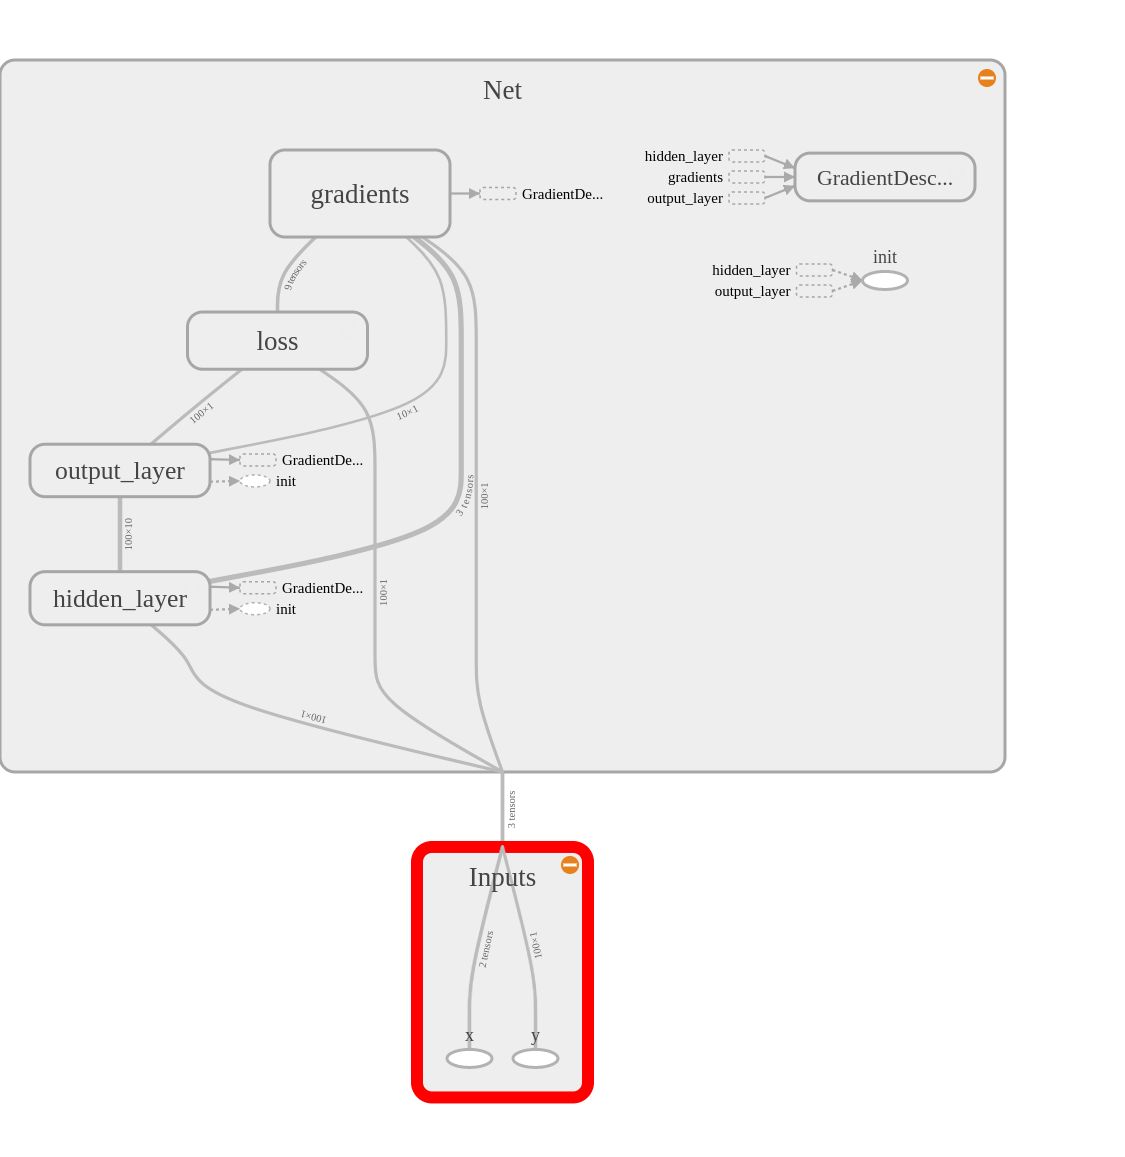
\includegraphics[scale=0.4]{./pic/chapter1/tenbor1.png}
\end{figure}
\subsection{TensorBoard Histogram Dashboard}
TensorBoard Histogram Dashboard 显示TensorFlow图中的Tensor如何随着时间变化。
\subsection{一个简单的例子}
正态分布变量,均值随着和时间移动。TensorFlow有一个操作tf.random\_normal可以完美的达到这个目的。正如通常情况下TensorBoard,我们将用summary op融合数据据。
在这种情况下'tf.summary.histogram'。
这里有一个代码段将生成一些包含正态分布直方图数据的总结,这里均值随着时间增大。
\begin{python}
import tensorflow as tf
k = tf.placeholder(tf.float32)
mean_moving_normal = tf.random_normal(shape=[1000], mean=(5*k), stddev=1)
summaries = tf.summary.histogram('normal/moving_mean',mean_moving_normal)
sess = tf.Session()
writer = tf.summary.FileWriter('./histogram_example')
N = 400
for step in range(N):
    k_val = step/float(N)
    summ = sess.run(summaries,feed_dict={k:k_val})
    writer.add_summary(summ,global_step=step)
\end{python}
在当前代码中运行下边的代码启动TensorFlow载入数据
\begin{python}
tensorboard --logdir=./histogram_example
\end{python}
\begin{center}
\begin{figure}[H]
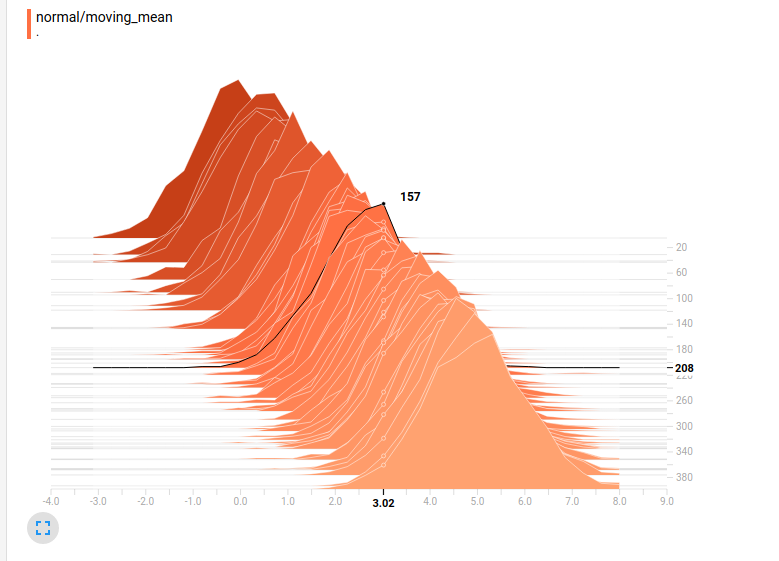
\includegraphics[scale=0.5]{tb_hist1.png}
\end{figure}
\end{center}
tf.summary.histogram接受任一尺寸和大小的Tensor,压缩他们进入直方数据结构组成一些小的数据宽度和数量组层的bin将诶够,例如我们像组成数[0.5,1.1,1.3,2.2,2.9,2.99]成3个bin,我们可以创建三个bin:一个包含0到1之间的一切(0.5),一个包含1-2(1.1,1.3)之间,一个包含2-3(2.2,2.9,2.99)

  TensorFlow用类是的方法创建bins,但是不想我们上面的例子,它不创建整数读额bins,瑞与大型数据,稀疏数据,这样的也许导致上千个bin,bins时指数分布时,一些bins相比于一些非常大数的bin接近于0。然而,可视化指数分布bin时一个技巧,如果高被编码为数量,bin宽度更大的空间,甚至他们有相同的元素,相比较之下统计数量使得豪赌比较变得可能,直方图采集数据仅均匀的bins,这可能导致不幸的人工操作。

在直方图可视化器的每一个切片显示为一个单个的直方图。切片安装步数组织。例老的切片(e.g. step 0)比较靠后变为更深,然而新的slices接近于前景色,颜色更轻,右边的y轴显示了步数。

你可以在直方图上滑动鼠标看到更多的详细星系。你如下面的图你可以看到直方图的时间不为177有一个bin中心在3.78有bin中有34.5个元素。
\begin{center}
\begin{figure}[H]
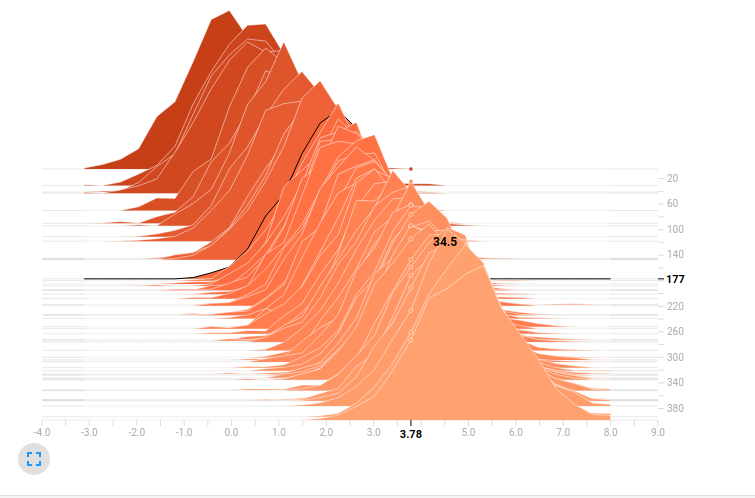
\includegraphics[scale=0.5]{tb_hist2.png}
\end{figure}
\end{center}
你也许注意到注意到直方切片在统计步数和时间上不总是偶数,这是因为TensorBoard用\href{https://en.wikipedia.org/wiki/Reservoir\_sampling}{reservoir sampling}保持直方图的子集,为了节约内存,Reservior sampling保证每个采样有一个相等的可能性被包含进去,但是因为它时一个随机算法,采样并不在每个偶数步发生。
\subsection{Overlay Mode}
控制面板上允许你打开直方图模式为offset为overlay。
在offset模式下,可视化转动45度,因此单个的直方图切片不再展开,而是所有的图华仔一个相同的y轴上。
\begin{center}
\begin{figure}[H]
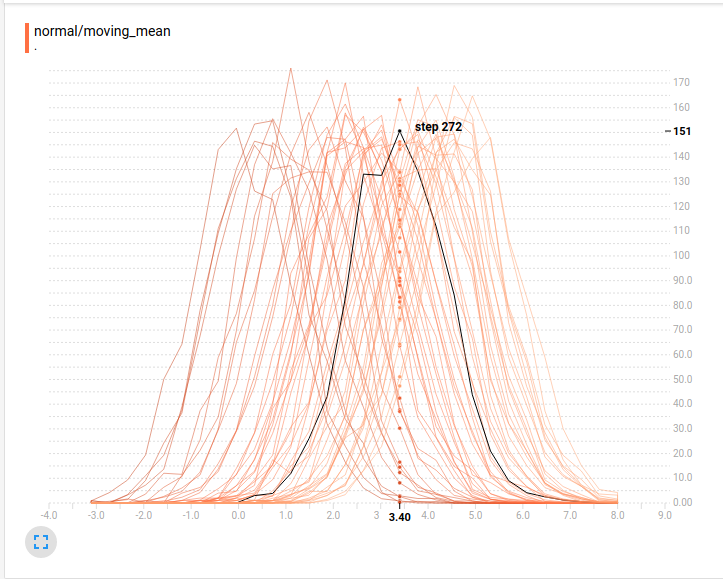
\includegraphics[scale=0.5]{tb_hist3.png}
\end{figure}
\end{center}
现在表上的每个切片被线分开,y轴显示每个bucket项目数量,深色线时老的,早期的时间不,浅色线时最近的新的时间不,你可以用鼠标在表上查看更多的信息。
\begin{center}
\begin{figure}[H]
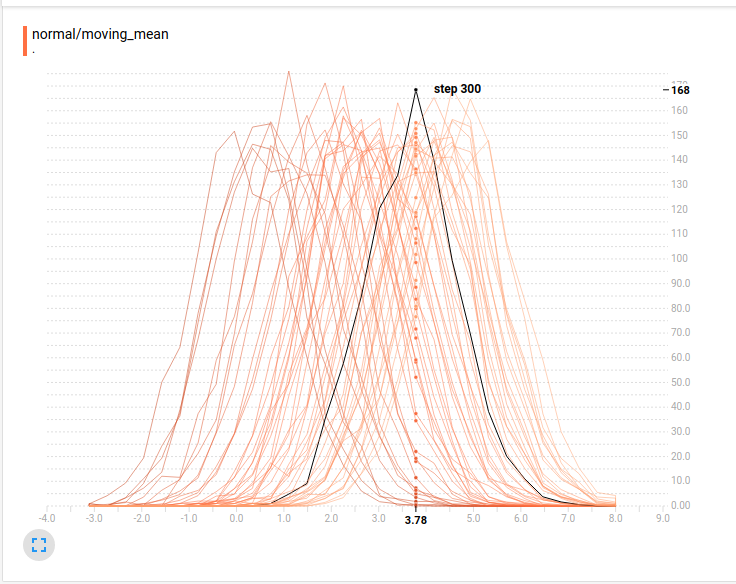
\includegraphics[scale=0.5]{tb_hist4.png}
\end{figure}
\end{center}

overlay可视化在你想直接比较不同直方图的数量。
\subsection{多个分布}
直方图控制面板对多分布下的可视化很有用,当我们通过链接两个不同的正态分布构造一个简单的二两分布,代码如下:
\begin{python}
import tensorflow as tf
k = tf.placeholder(tf.float32)
mean_moving_normal = tf.random_normal(shape=[1000],mean=(3*5),stddev=1)
tf.summary.histogram('normal/moving_mean',mean_moving_normal)
variance_shrinking_normal = tf.random_normal(shape=[100],mean=0,stddev=1-(k))
tf.summary.histogram('normal/shrinking_varance',variance_shrinking_normal)
normal_combined = tf.concat([mean_moving_normal,variance_shrinking_normal],0)
tf.summary.histogram('normal/bimodal',normal_combined)
summaris = tf.summary.merge_all()
sess = tf.Session()
writer = tf.summary.FileWriter('./histgram_example1')
N = 400
for step in range(N):
    k_val = step/float(N)
    summ = sess.run(summaris,feed_dict={k:k_val})
    writer.add_summary(summ,global_step=step)
\end{python}
上面的例子是滑动平均,现在我们已有一个收缩的变量分布。
\begin{center}
\begin{figure}[H]
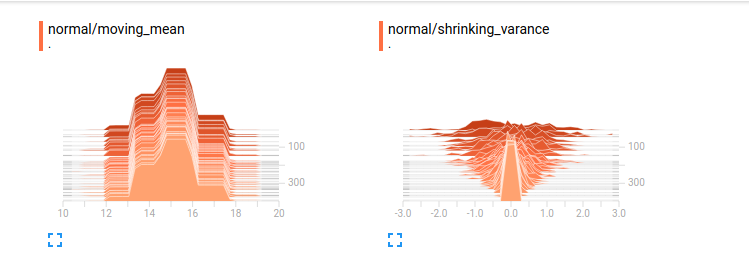
\includegraphics[scale=0.6]{tb_hist5.png}
\end{figure}
\end{center}
当我们链接她们在一起,我们得到一个清晰解释分歧,二进制结构的表格:
\begin{center}
\begin{figure}[H]
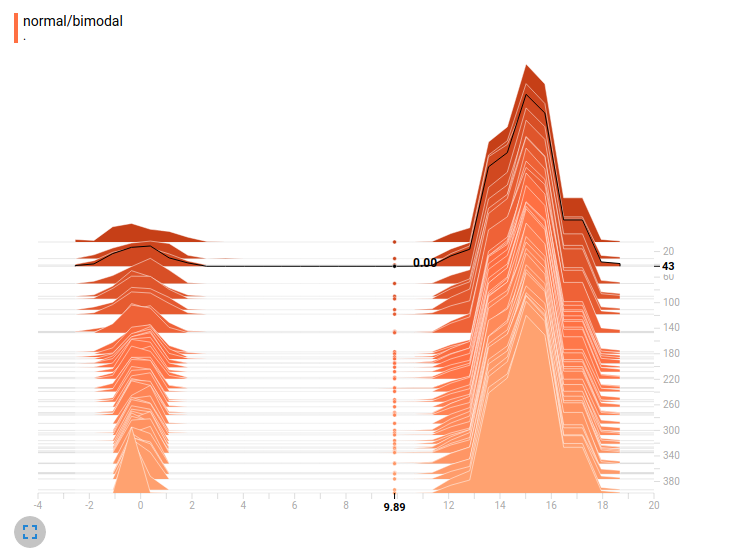
\includegraphics[scale=0.5]{tb_hist6.png}
\end{figure}
\end{center}
\subsection{更多分布}
生成可视化更多分布,结合他们到表中:
\begin{python}
import tensorflow as tf
k = tf.placeholder(tf.float32)
# Make a normal distribution,with a shift mean
mean_moving_normal = tf.random_normal(shape=[1000],mean=(5*k),stddev=1)
tf.summary.histogram('normal/moving_mean',mean_moving_normal)
variance_shrinking_normal = tf.random_normal(shape=[1000],mean=0,stddev=1-(k))
tf.summary.histogram('normal/shinking_variance',variance_shrinking_normal)
normal_combined = tf.concat([mean_moving_normal,variance_shrinking_normal],0)
tf.summary.histogram("normal/bimodal",normal_combined)
#add gamma distribution
gamma = tf.random_gamma(shape=[1000],alpha=k)
tf.summary.histogram('gamma',gamma)
poisson = tf.random_poisson(shape=[1000],lam=k)
tf.summary.histogram('poisson',poisson)
#add a uniform distribution
uniform = tf.random_uniform(shape=[1000],maxval=k*10)
tf.summary.histogram('uniform',uniform)
#finnally combine everything together

all_distributions = [mean_moving_normal,variance_shrinking_normal,gamma,poisson,uniform]
all_combined = tf.concat(all_distributions,0)
tf.summary.histogram('all_combined',all_combined)
summaries = tf.summary.merge_all()
sess = tf.Session()
writer = tf.summary.FileWriter('./histogram_example2')
N = 400
for step in range(N):
    k_val = step/float(N)
    summ = sess.run(summaries,feed_dict={k:k_val})
    writer.add_summary(summ,global_step=step)
\end{python}
\begin{center}
\begin{figure}[H]
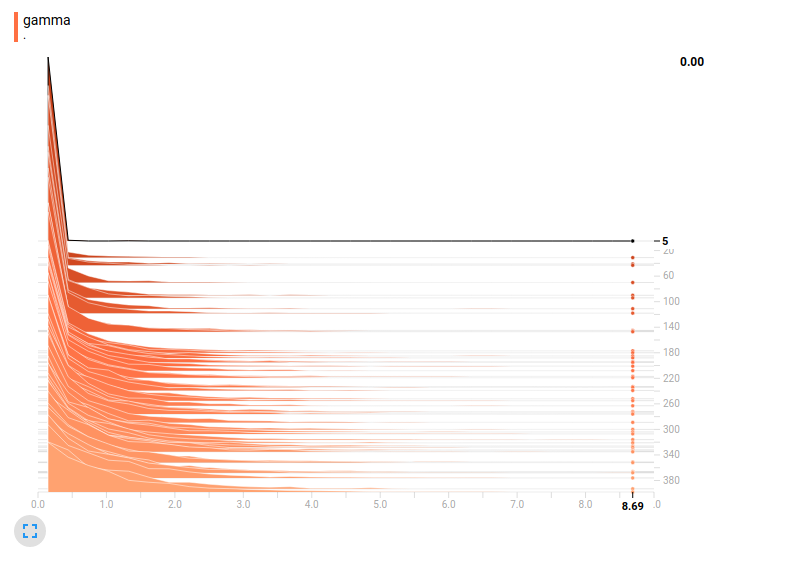
\includegraphics[scale=0.5]{tb_hist7.png}
\end{figure}
\end{center}
\begin{center}
\begin{figure}
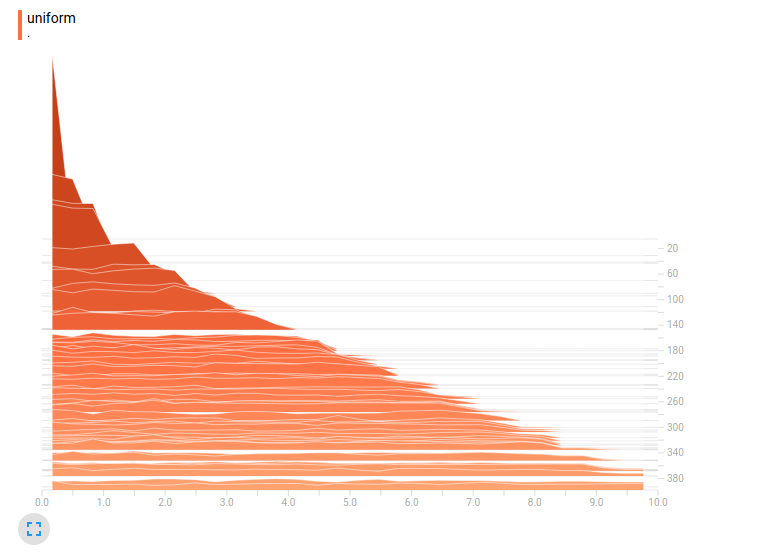
\includegraphics[scale=0.5]{tb_hist9.png}
\end{figure}
\end{center}
\subsection{poisson分布}
\begin{center}
\begin{figure}[H]
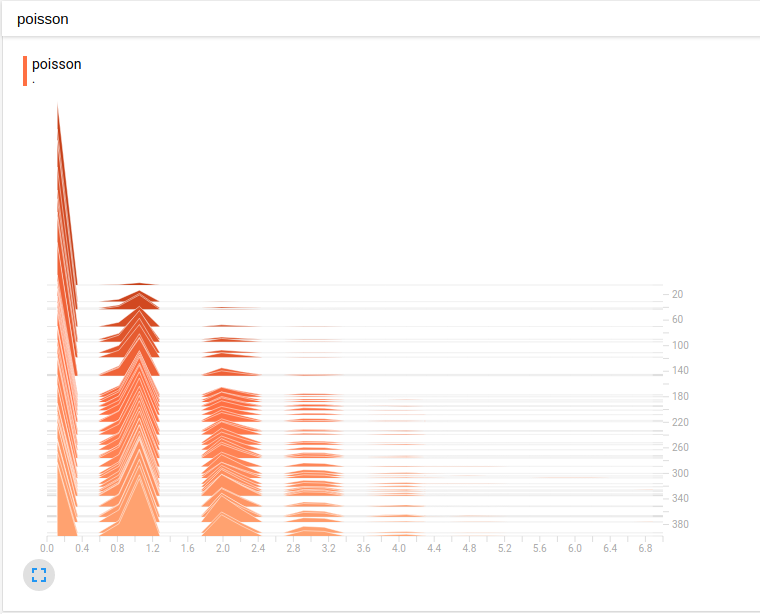
\includegraphics[scale=0.5]{tb_hist10.png}
\end{figure}
\end{center}
poisson分布定义在整数上,因此所有被生成的值都是整数,直方图压缩移动数据到浮点bins,导致可视化在整数值上显示一点点突起。
\subsection{结合所有的数据到一张图向上}
\begin{center}
\begin{figure}[H]
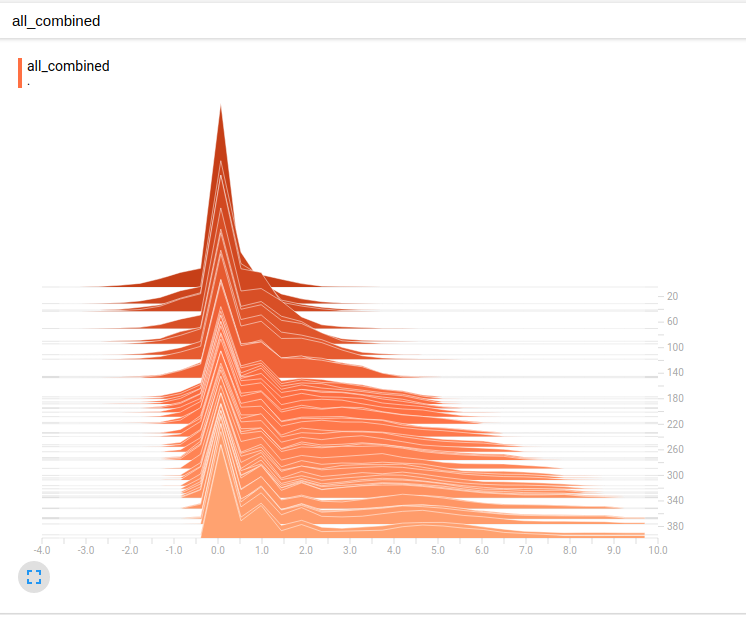
\includegraphics[scale=0.5]{tb_hist11.png}
\end{figure}
\end{center}


\begin{python}
import tensorflow as tf
import matplotlib.pyplot as plt
import numpy as np
tf.set_random_seed(0)
np.random.seed(0)
x = np.linspace(-1,1,100).reshape(-1,1)
noise = np.random.normal(0,0.1,size=x.shape)
y = np.power(x,2)+noise
def gendata():
    t = np.linspace(-1,1,100).reshape(-1,1)
def save():
    print('This is save')
    tf_x = tf.placeholder(tf.float32,x.shape)
    tf_y = tf.placeholder(tf.float32,y.shape)
    l = tf.layers.dense(tf_x,10,tf.nn.relu)
    o = tf.layers.dense(l,1)
    loss = tf.losses.mean_squared_error(tf_y,o)
    train_op = tf.train.GradientDescentOptimizer(learning_rate=0.5).minimize(loss)
    sess = tf.Session()
    sess.run(tf.global_variables_initializer())
    saver = tf.train.Saver()
    for step in range(100):
        sess.run(train_op,{tf_x:x,tf_y:y})
    saver.save(sess,'params',write_meta_graph=False)
    pred,l = sess.run([o,loss],{tf_x:x,tf_y:y})
    plt.figure(1,figsize=(10,5))
    plt.subplot(121)
    plt.scatter(x,y)
    plt.plot(x,pred,'r-',lw=5)
    plt.text(-1,1.2,'save loss=%.4f'%l,fontdict={'size':15,'color':'red'})
def reload():
    print('This is reload')
    tf_x = tf.placeholder(tf.float32,x.shape)
    tf_y = tf.placeholder(tf.float32,y.shape)
    l_ = tf.layers.dense(tf_x,10,tf.nn.relu)
    o_ = tf.layers.dense(l_,1)
    loss_ = tf.losses.mean_squared_error(tf_y,o_)
    sess = tf.Session()
    saver = tf.train.Saver()
    saver.restore(sess,'params')
    pred,l = sess.run([o_,loss_],{tf_x:x,tf_y:y})
    plt.subplot(122)
    plt.scatter(x,y)
    plt.plot(x,pred,'r-',lw=5)
    plt.text(-1,1.2,'Reload Loss=%.4f'%l,fontdict={'size':15,'color':'red'})
    plt.show()
save()
tf.reset_default_graph()
reload()
\end{python}
\section{CNN手写体数据识别}
\subsection{mnist数据集}
手写体数据训练集有55000张手写体数据图片。测试集有10000张图片。每张图片是大小为32*32的灰度图片。
卷积神经网络结构:
\begin{itemize}
	\item 第一层卷积层:卷积核16个,卷积核大小为$5\times5$,strides=1,padding为SAME,激活函数为relu(输出大小为$28\times28\times16$)。
	\item 第一层池化层:池化层大小为2,strides为2($14\times14\times16$)。
第二层卷积层:卷积核32,大小为$5\times5$,strides=1,padding为SAME,激活函数为relu。($14\times14\times32$)
	\item 第二层池化层:池化层大小为2,strides为2($7\times7\times32$)。
	\item flatten:1568。
\end{itemize}
\begin{figure}[H]
	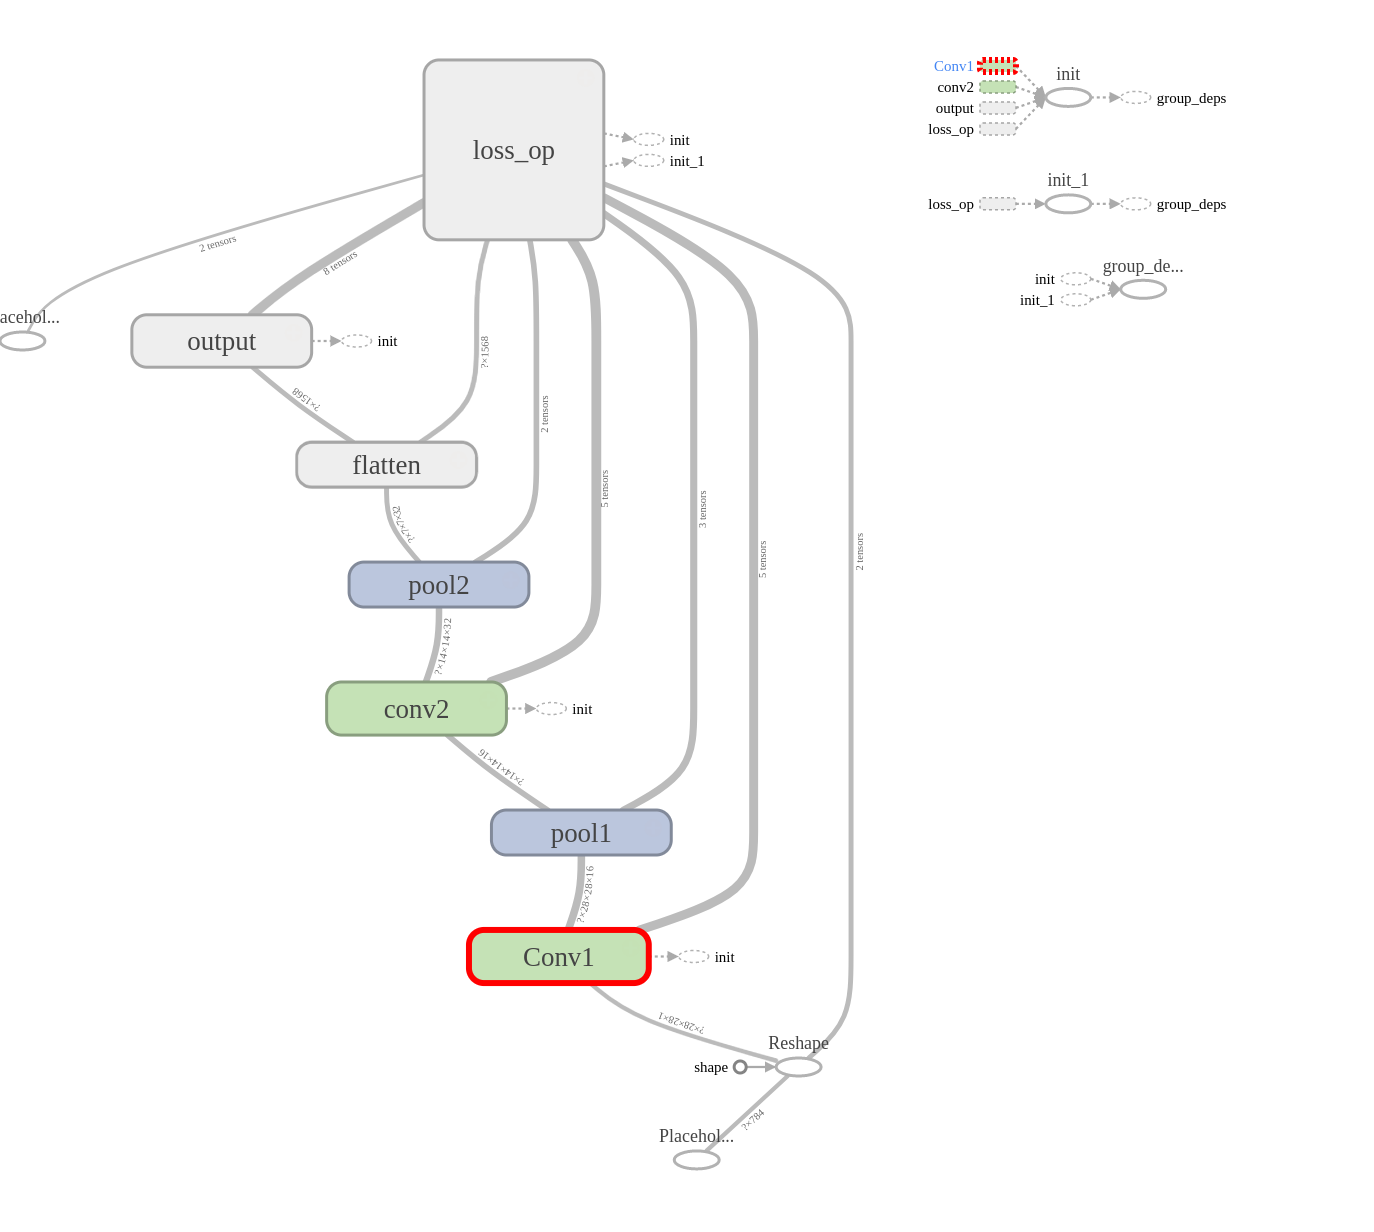
\includegraphics[scale=0.4]{./pic/chapter1/mnist_cnn.png}
\end{figure}
\begin{python}
import tensorflow as tf
import matplotlib.pyplot as plt
import numpy as np
from tensorflow.examples.tutorials.mnist import input_data

tf.set_random_seed(0)
np.random.seed(0)

BATCH_SIZE = 50
LR = 0.001
mnist = input_data.read_data_sets('/home/hpc/文档/mnist_tutorial/mnist',one_hot = True)
test_x = mnist.test.images[:2000]
test_y = mnist.test.labels[:2000]

tf_x = tf.placeholder(tf.float32,[None,28*28])
images = tf.reshape(tf_x,[-1,28,28,1])
tf_y = tf.placeholder(tf.int32,[None,10])
with tf.variable_scope('Conv1'):
    conv1 = tf.layers.conv2d(
            inputs = images,
            filters = 16,
            kernel_size = 5,
            strides = 1,
            padding = 'same',
            activation = tf.nn.relu
        )
    tf.summary.histogram('conv1',conv1)
with tf.variable_scope('pool1'):
    pool1 = tf.layers.max_pooling2d(
            conv1,
            pool_size=2,
            strides =2
        )
    tf.summary.histogram('max_pool1',pool1)
with tf.variable_scope('conv2'):
    conv2 = tf.layers.conv2d(pool1,32,5,1,'SAME',activation=tf.nn.relu)
    tf.summary.histogram('conv2',conv2)
with tf.variable_scope('pool2'):
    pool2 = tf.layers.max_pooling2d(conv2,2,2)
    tf.summary.histogram('max_pool',pool2)
with tf.variable_scope('flatten'):
    flat = tf.reshape(pool2,[-1,7*7*32])
with tf.variable_scope('output'):
    output = tf.layers.dense(flat,10)
with tf.variable_scope('loss_op'):
    loss = tf.losses.softmax_cross_entropy(onehot_labels=tf_y,logits=output)
    train_op = tf.train.AdamOptimizer(LR).minimize(loss)
    accuracy = tf.metrics.accuracy(labels = tf.argmax(tf_y,axis=1),predictions=tf.argmax(output,axis=1),)[1]
    tf.summary.scalar('loss',loss)
    tf.summary.scalar('accuracy',accuracy)
sess = tf.Session()
merge_op = tf.summary.merge_all()
init_op = tf.group(tf.global_variables_initializer(),tf.local_variables_initializer())
sess.run(init_op)
writer = tf.summary.FileWriter('./log',sess.graph)
for step in range(600):
    b_x,b_y = mnist.train.next_batch(BATCH_SIZE)
    _,loss_,result = sess.run([train_op,loss,merge_op],{tf_x:b_x,tf_y:b_y})
    writer.add_summary(result,step)
    if step%50 == 0:
        accuracy_,flat_representation = sess.run([accuracy,flat],{tf_x:test_x,tf_y:test_y})
        print('Step:',step,'| train loss:%.4f'%loss_,'|test accuracy:%.2f'%accuracy_)
test_output = sess.run(output,{tf_x:test_x[:10]})
pred_y = np.argmax(test_output,1)
\end{python}
\section{RNN}
人不能抓住每一秒的思考,当你读这篇文章的时候,你能基于你之前的对单词的理解明白文章的每一个单词的意思,你思考的时候不需要丢掉所有的东西,你的思想有持续性。\par
传统的神经网络很难做到这点,这也是传统神经网络的主要缺点。例如你想分类电影中的不同时间点的事件,传统神经网络用不清楚如何用之前的事件了解新的事件。\par
RNN通过循环处理这个问题,允许信息保留。\par
\begin{figure}[!ht]
\centering
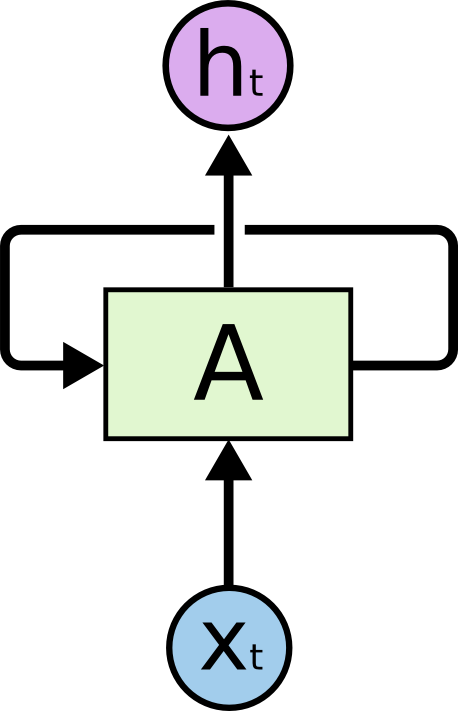
\includegraphics[scale=0.5]{RNN-rolled.png}
\end{figure}
上面的图表示一个RNN单元,A得到输入$x_t$和输出$h_t$,A允许信息被循环从一步到下一步,一个循环神经网络可以看成是多个相同单元的复制。铺开RNN可以得到
\begin{figure}[!ht]
\centering
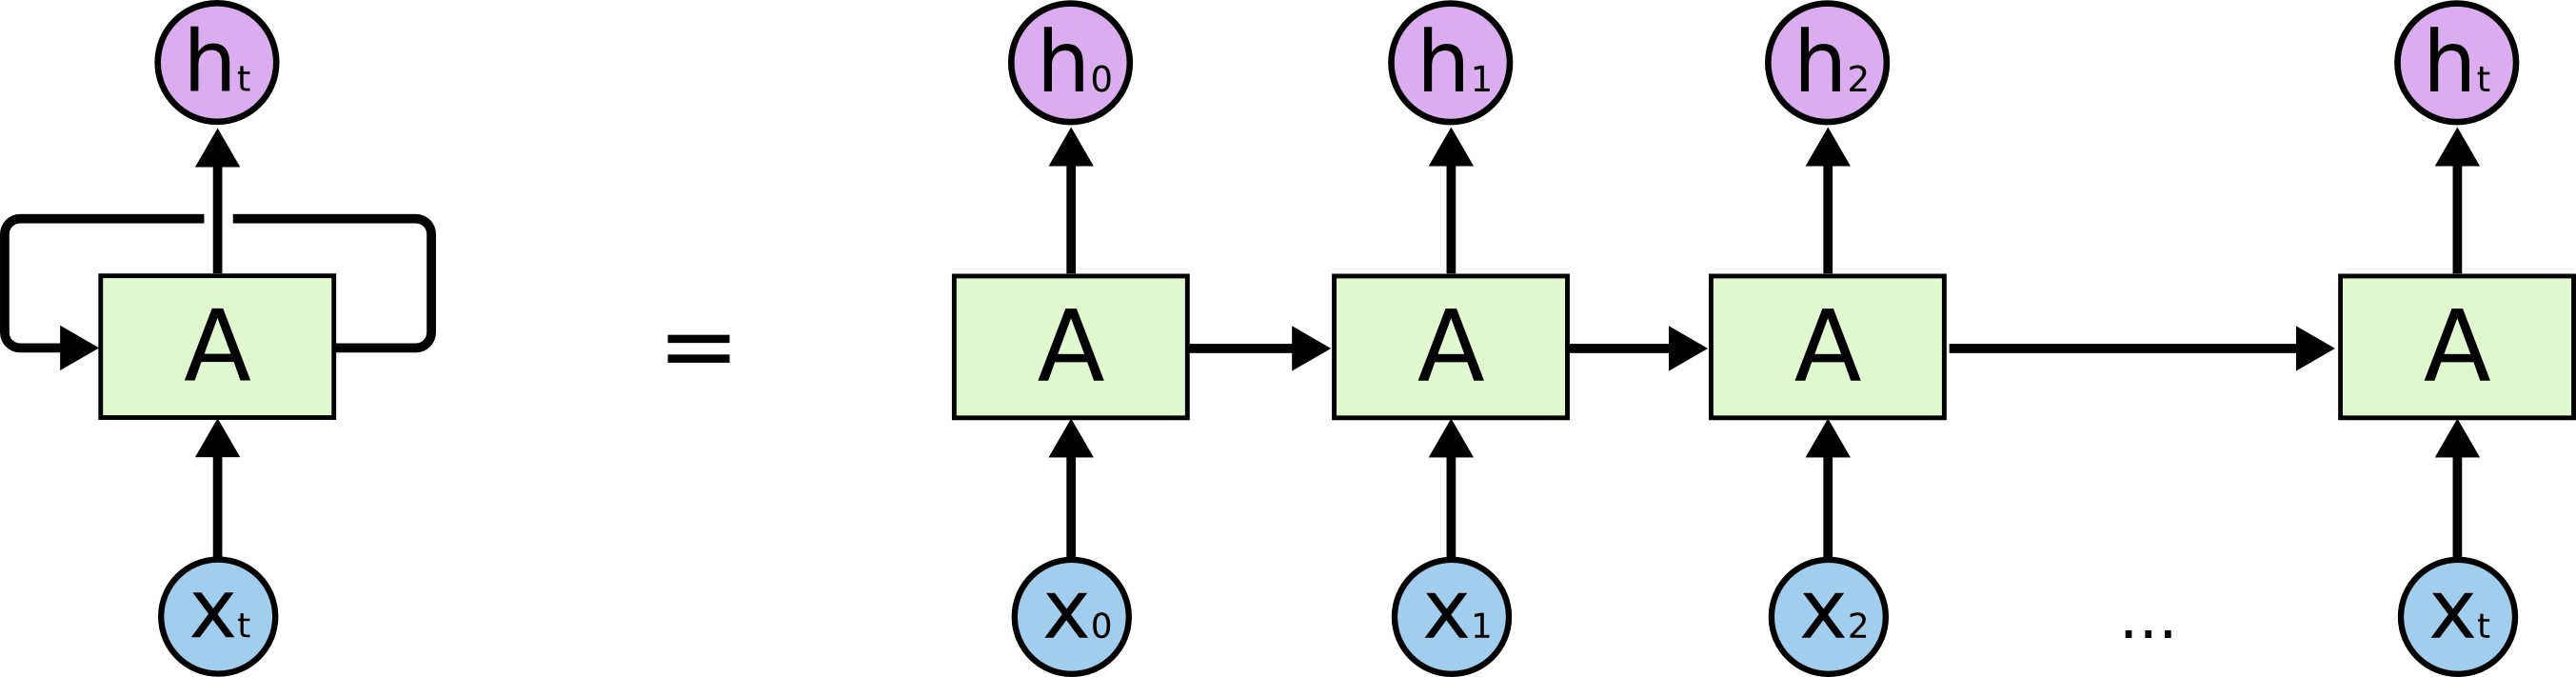
\includegraphics[scale=0.3]{RNN-unrolled.png}
\caption{unrolled RNN}
\end{figure}
这个链式结构揭示了循环神经网络和序列或者列表密切相关,它适用于这种数据。
\subsection{The Problem Long-Term Dependencies}
语言模型中常用先前的一个词预测下一个词,如果我们尝试预测"the clouds are in the {\color{red}{sky}}"我们不需要很多上下文信息RNN通过之前的信息就能学到。但是我们尝试预测这样一个句子"I grew up in France... I speak fluent {\color{red}{France}}",之前的信息暗示下一个单词可能是语言的名字,如果我们想去缩小语言的范围,我们需要上下文{\color{red}{France}},可相关信息和这个需要点的间隔很大。
\begin{figure}[!ht]
\centering
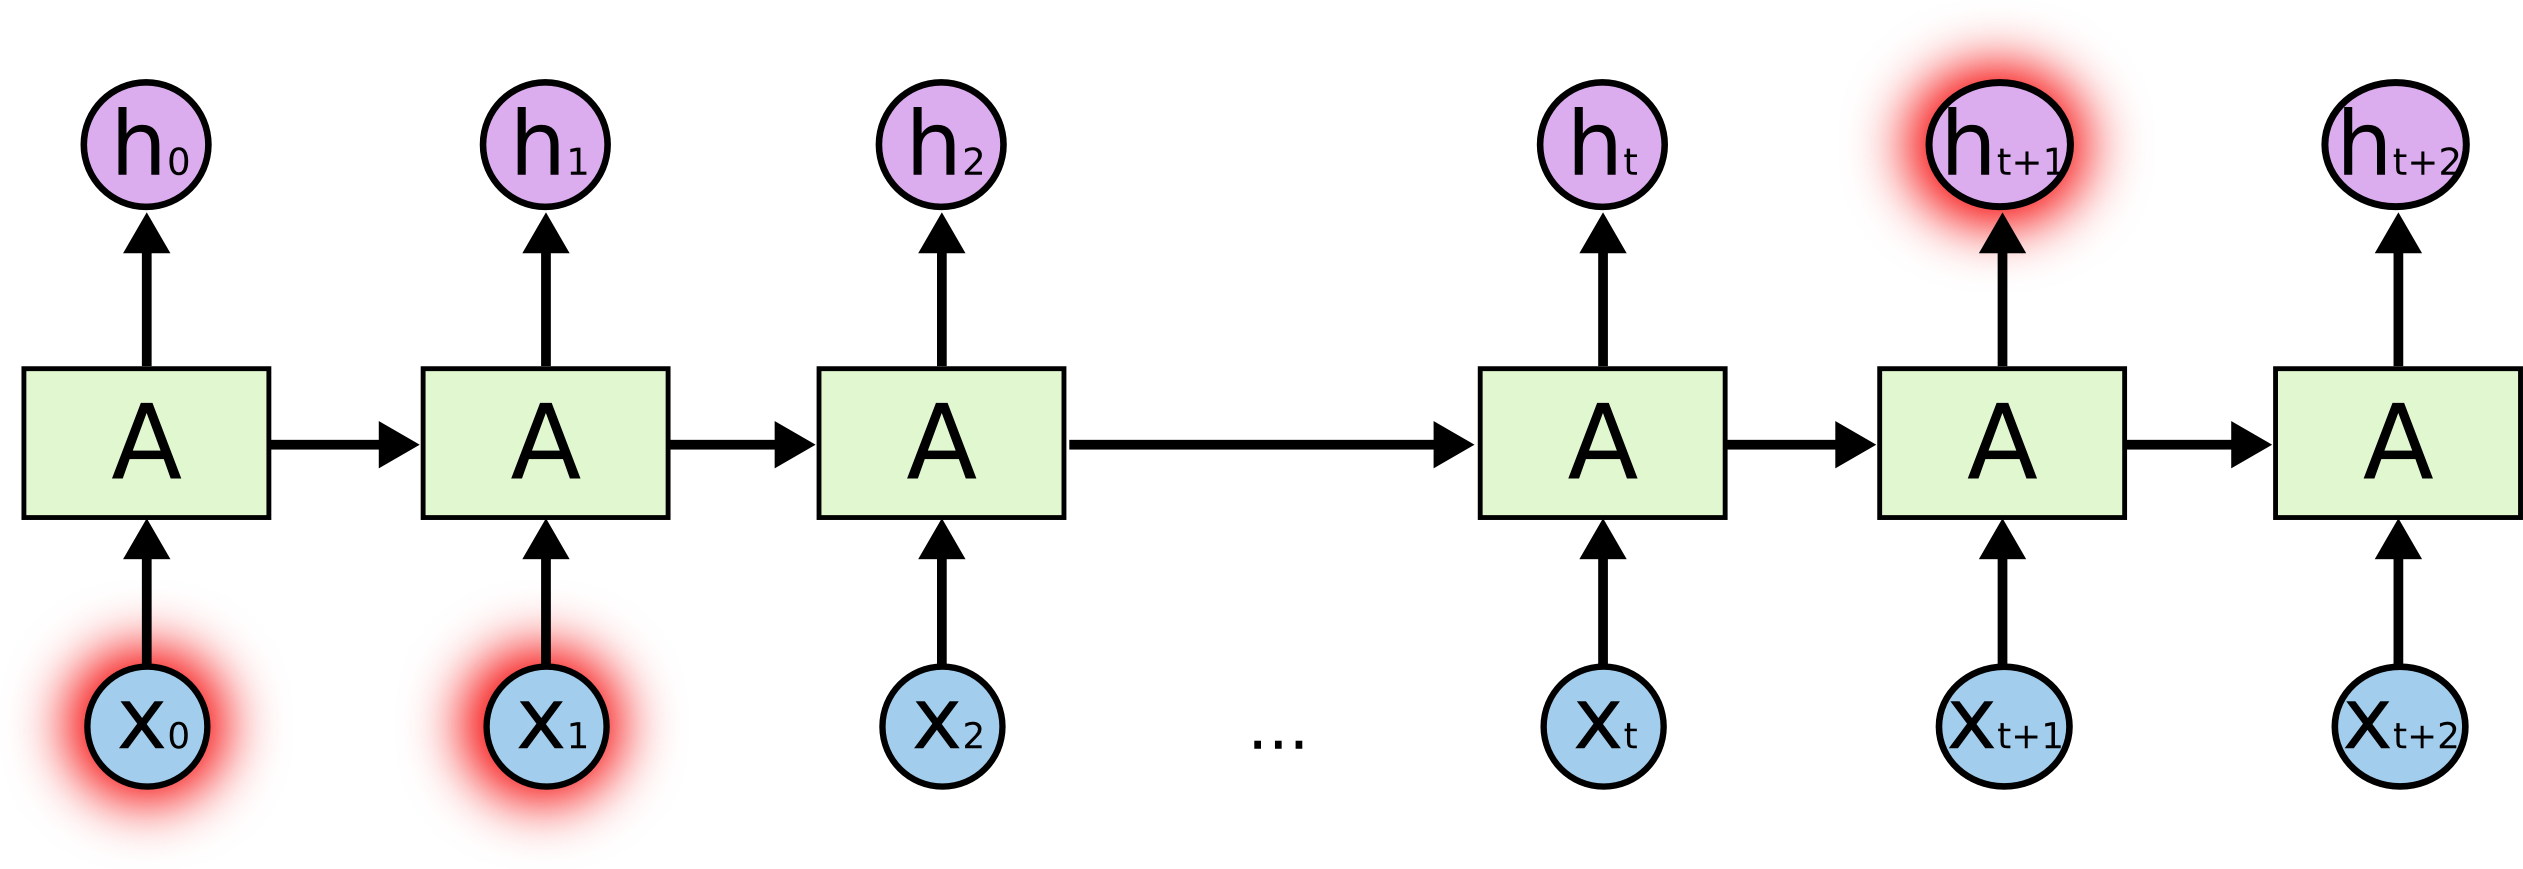
\includegraphics[scale=0.3]{RNN-longtermdependencies.png}
\end{figure}
理论上RNN有能力处理“long-term dependencies”,人能小心的挑选参数解决这个烦人的问题,然而不幸的是RNN似乎不能做到,原因由\href{http://www-dsi.ing.unifi.it/~paolo/ps/tnn-94-gradient.pdf}{Hochreiter (1991) [German] and Bengio, et al. (1994)}提出.
\subsection{LSTM网络}
Long Short Term Memory networks通常简称为LSTMs是一个特殊的RNN,能学习learning long-term dependencies,他被\href{http://deeplearning.cs.cmu.edu/pdfs/Hochreiter97_lstm.pdf}{Hochreiter  Schmidhuber (1997)}引入,然后被提炼,在大型文体处理上效果很好因而被广泛的使用。\par
LSTMs明确的设计去解决 long-term dependency problem。\par
所有的循环神经网络都有重复的链式形式。在标准的RNNs,重复的模块有一个非常简单的结构,像tanh Layer。
\begin{figure}
\centering
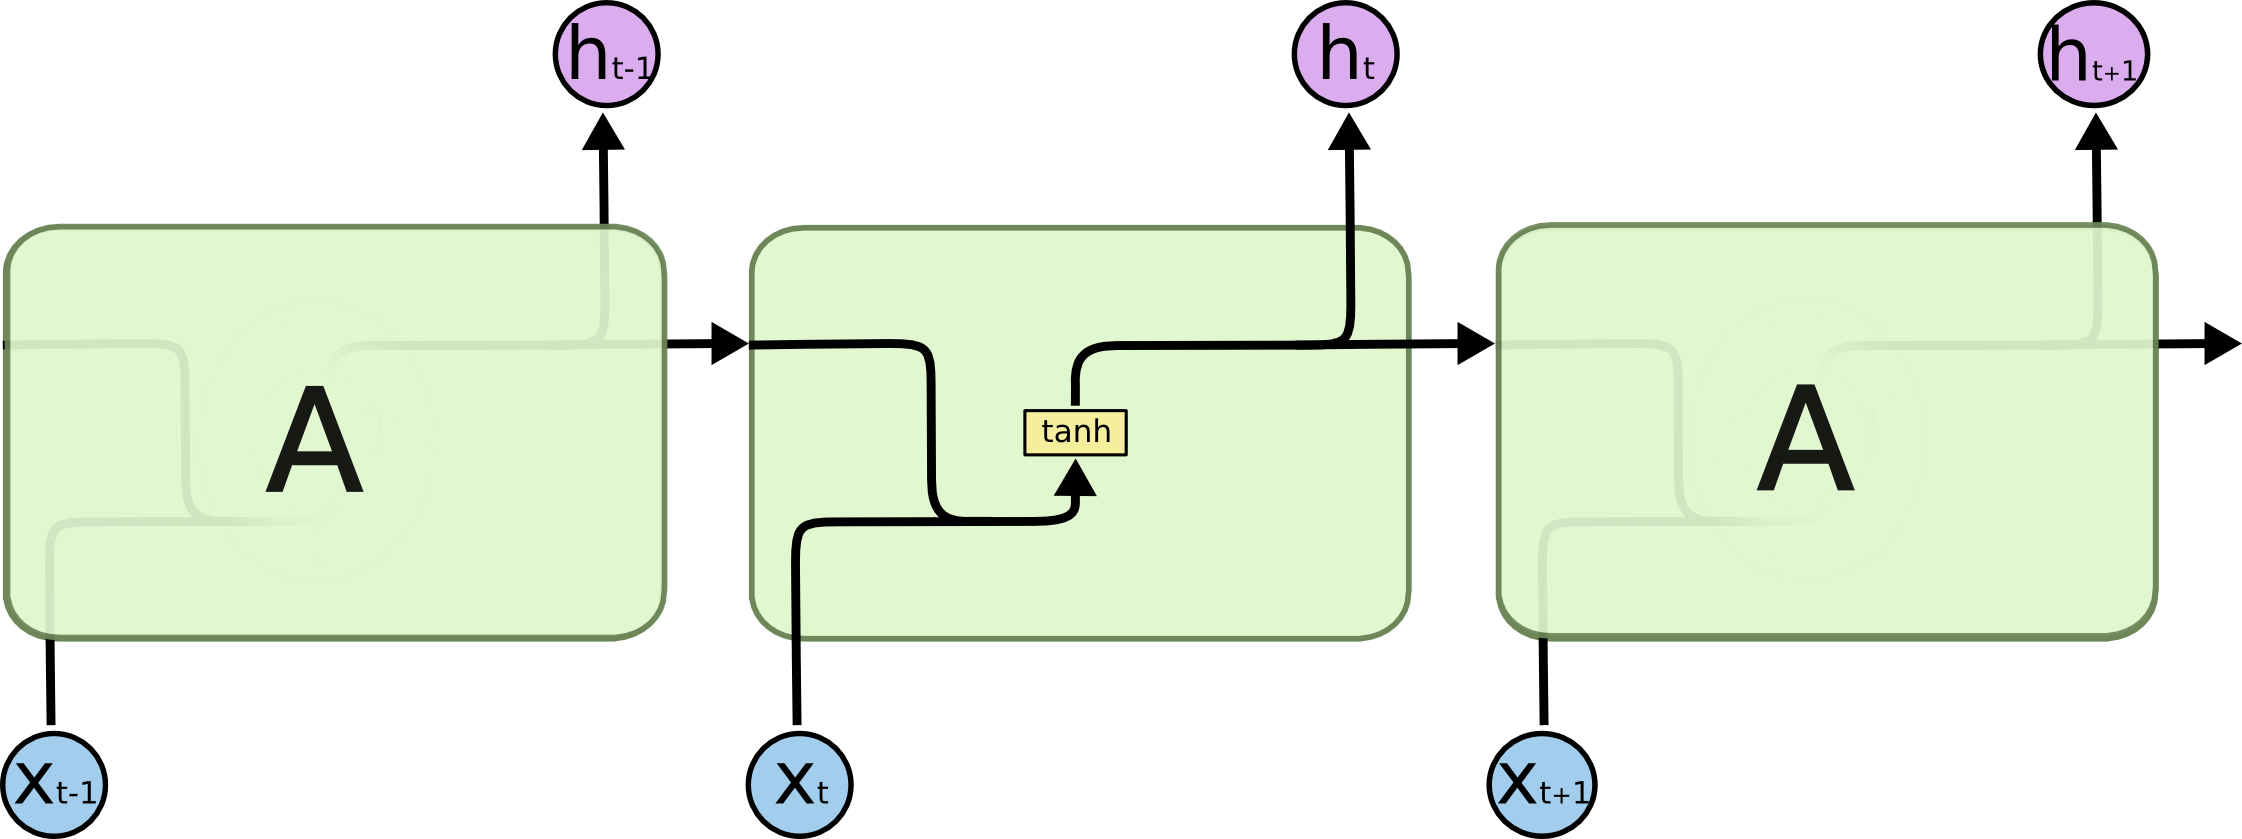
\includegraphics[scale=0.3]{LSTM3-SimpleRNN.png}
\caption{The repeating module in a standard RNN contains a single layer}
\end{figure}
LSTMs也有这样类似的结构,但是congruent模块有点不同,有一个神经网络层有四个相互作用部分,
\begin{figure}
\centering
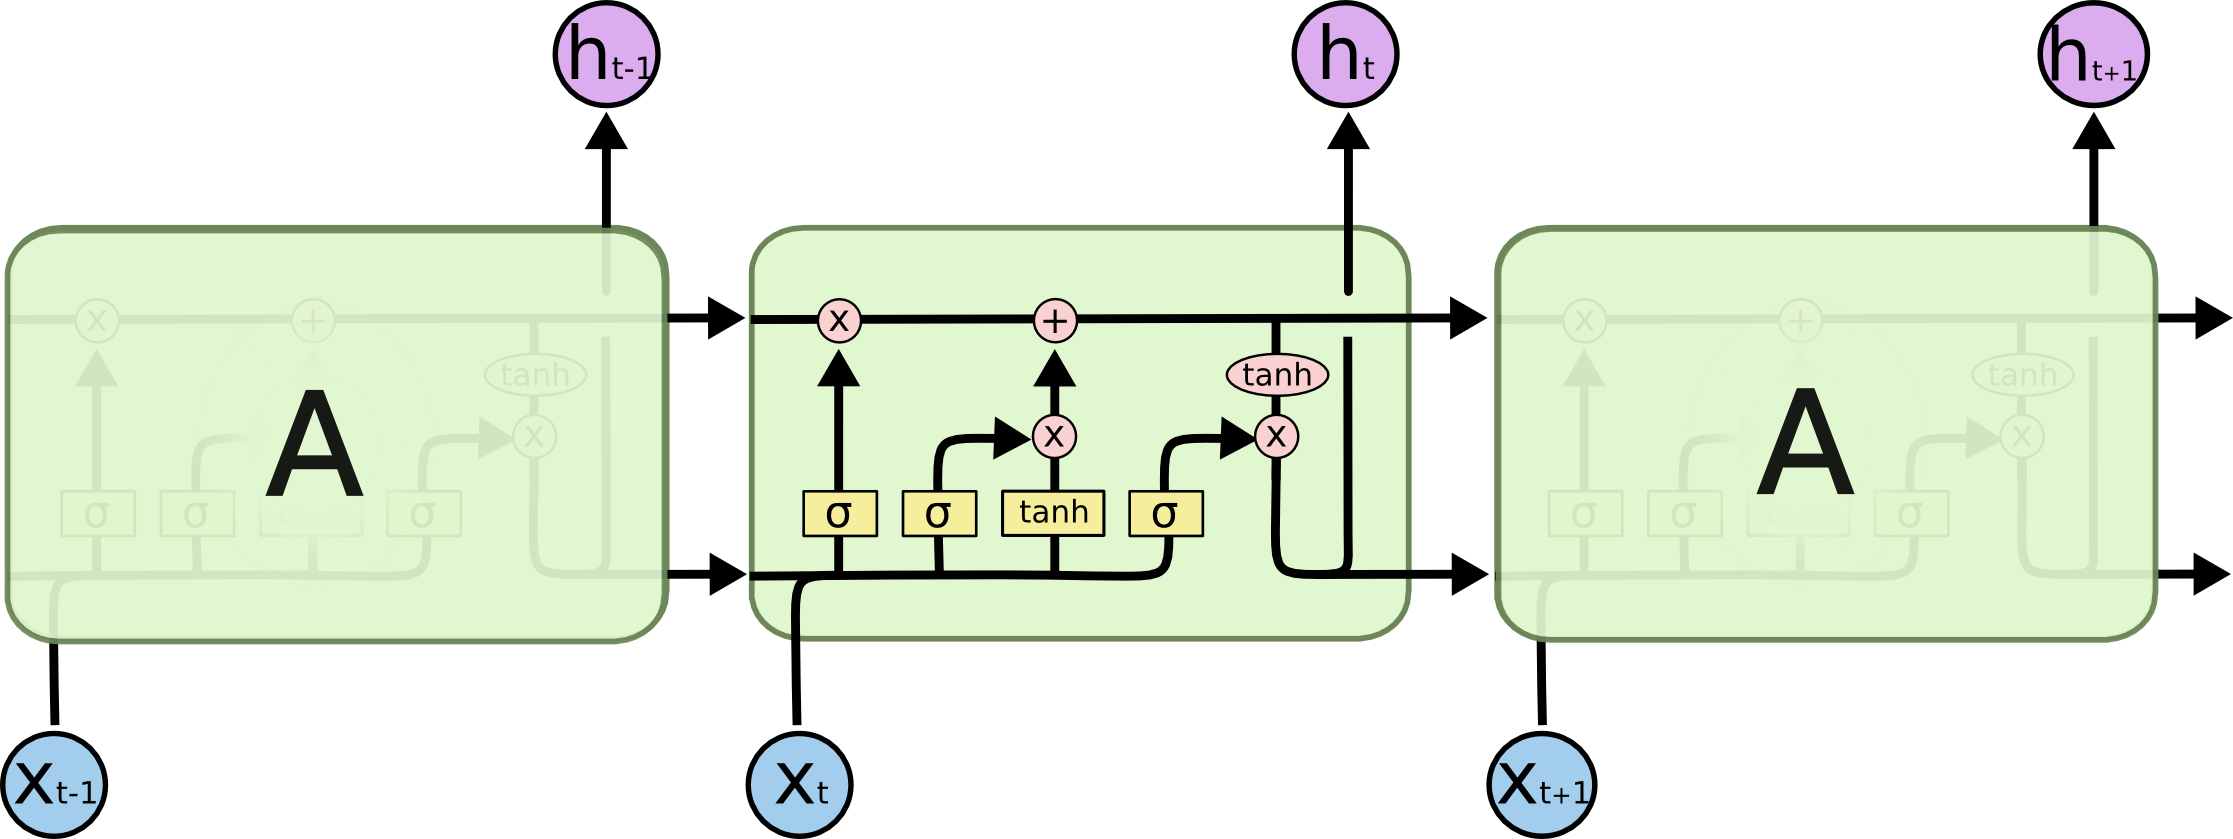
\includegraphics[scale=0.3]{LSTM3-chain.png}
\caption{The repeating module in an LSTM contains four interacting layers}
\end{figure}
\begin{figure}
\centering
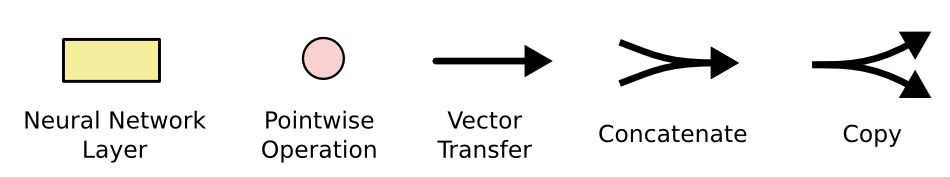
\includegraphics[scale=0.3]{LSTM2-notation.png}
\end{figure}
在上面的图上,每一根线上携带的都是一个向量,从一个输出节点到其他输入,粉色圆圈代表按点操作,黄色盒子是学习好的神经网络层,线融合表示串联,copy表示将一条线复制一份。
\subsection{LSTMs想法的核心}
LSTMs的核心是图像顶部的水平流过的cell state,cell state像一个传送带,它笔直的沿着整条链跑,和一些次要的线性交互,很容易实现信息不改变的流动。
\begin{figure}
\centering
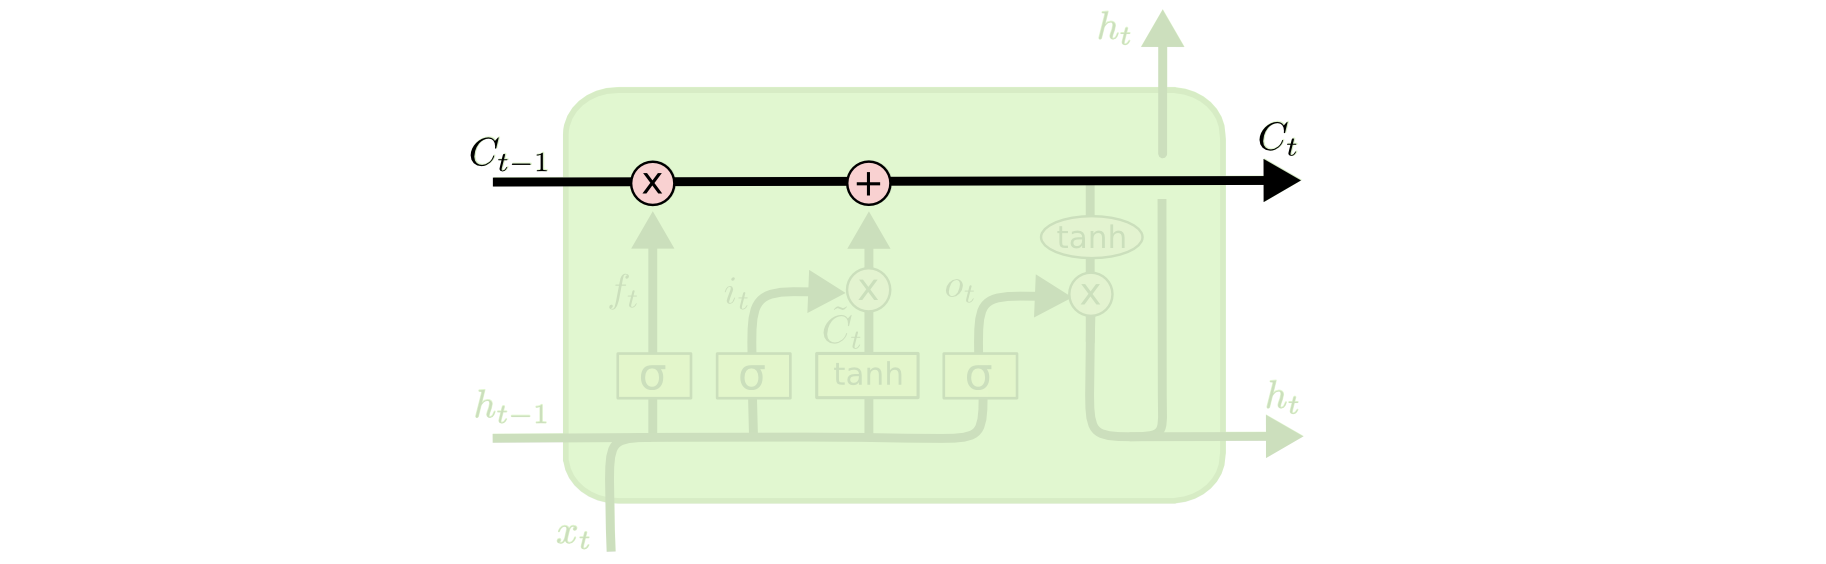
\includegraphics[scale=0.3]{LSTM3-C-line.png}
\end{figure}
LSTM能删除或者增加信息到cell state,被控制的结构称为门。门是一种让信息通过的手段,由一个sigmoid神经网络层和pointwise惩罚操作组成。
\begin{figure}
\centering
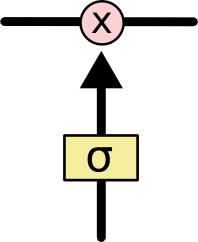
\includegraphics[scale=0.5]{LSTM3-gate.png}
\end{figure}
sigmod Layer输出0到1之间的数,描述多少组件应该被通过,0表示不允许通过1表示让一切通过,LSTMs有三个门,保护和控制cell state。
\subsection{一步步的设置}
第一步是LSTMs决定什么信息应该被传送,这个决定每一个称为忘记门的sigmoid layer组成,通过$h_{t-1}$和$x_t$输出0到1之间的数给当前的$C_{t-1}$,1表示完全保持,0表示丢弃。\par
对于上面的语言模型,cell state也许包含the gender of the present subjects,以至于正确的带名字能被使用,当我们看一个新的subject,我们想图忘记the gender of the old subject。
\begin{figure}
\centering
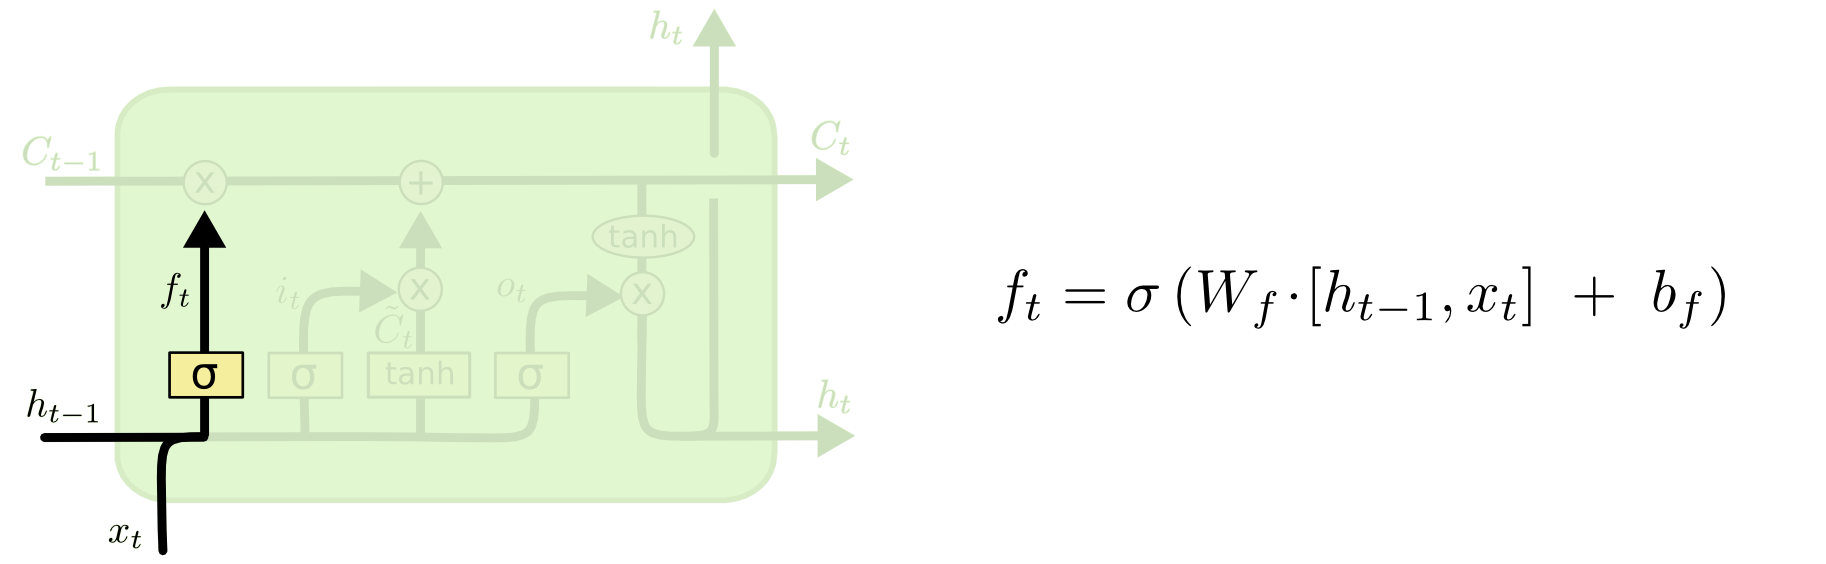
\includegraphics[scale=0.5]{LSTM3-focus-f.png}
\end{figure}
下一步是决定什么新的信息将被存储在cell state中,这分为两部分
\begin{enumerate}
	\item Sigmod layer调用 input gate layer决定更新哪个值。
	\item tanh layer创建一个可能被添加到state新的候选向量。$\widetilde{C_t}$
\end{enumerate}
下一步我们结合两个不走创建一个更新状态。,在我们的语言模型例子中,我们想要增加gender of the new subject到cell state取代我们将要忘记的数据
\begin{figure}
\centering
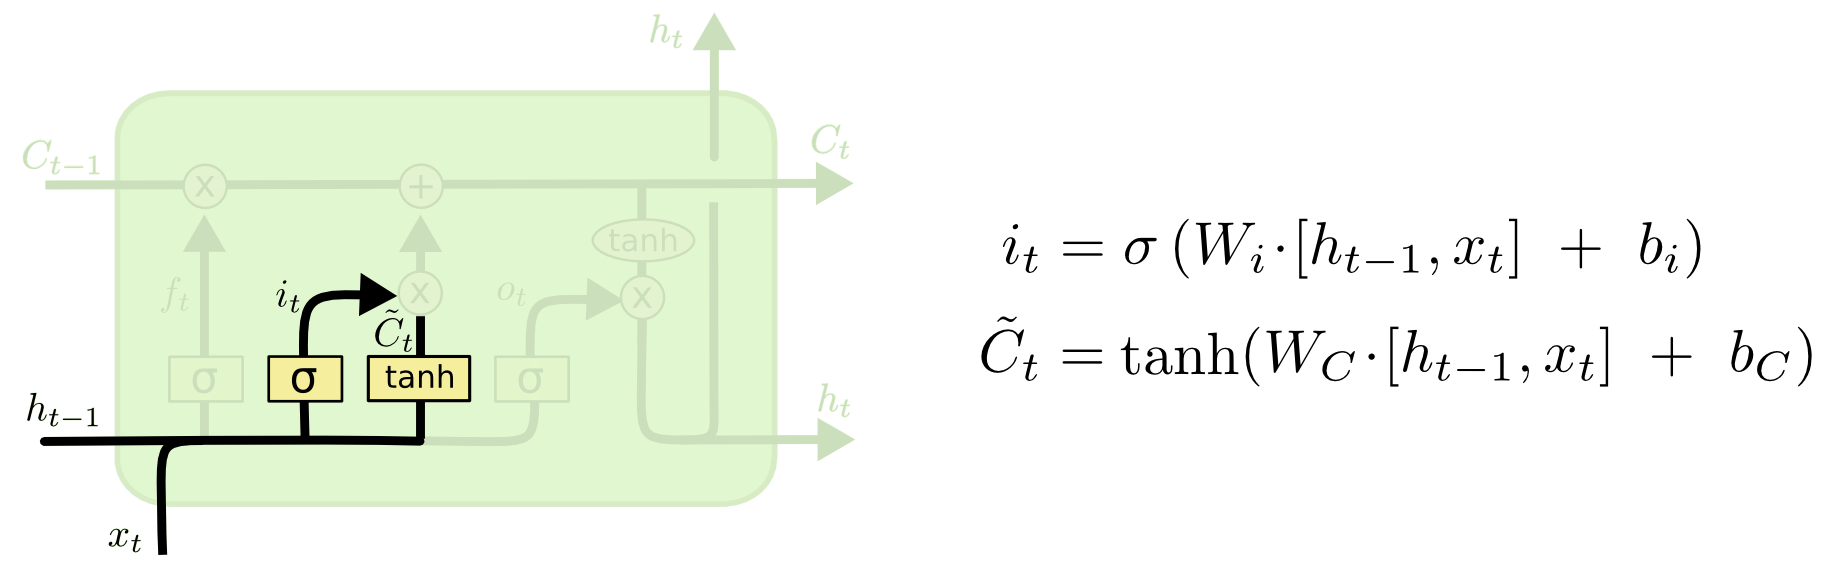
\includegraphics[scale=0.5]{LSTM3-focus-i.png}
\end{figure}
现在更新老的cell state$C_{t-1}$到新的cell state$C_t$,我们用老的$c_{t-1}$乘上$f_t$忘记我们之前决定忘记的事,然后我们增加$i_t*\widetilde{C_t}$.这是新的候选值,表示我们更新每个状态值的规模。在例子中的语言模型,我们删掉了一个老的subject's gender增加新的信息。
\begin{figure}
\centering
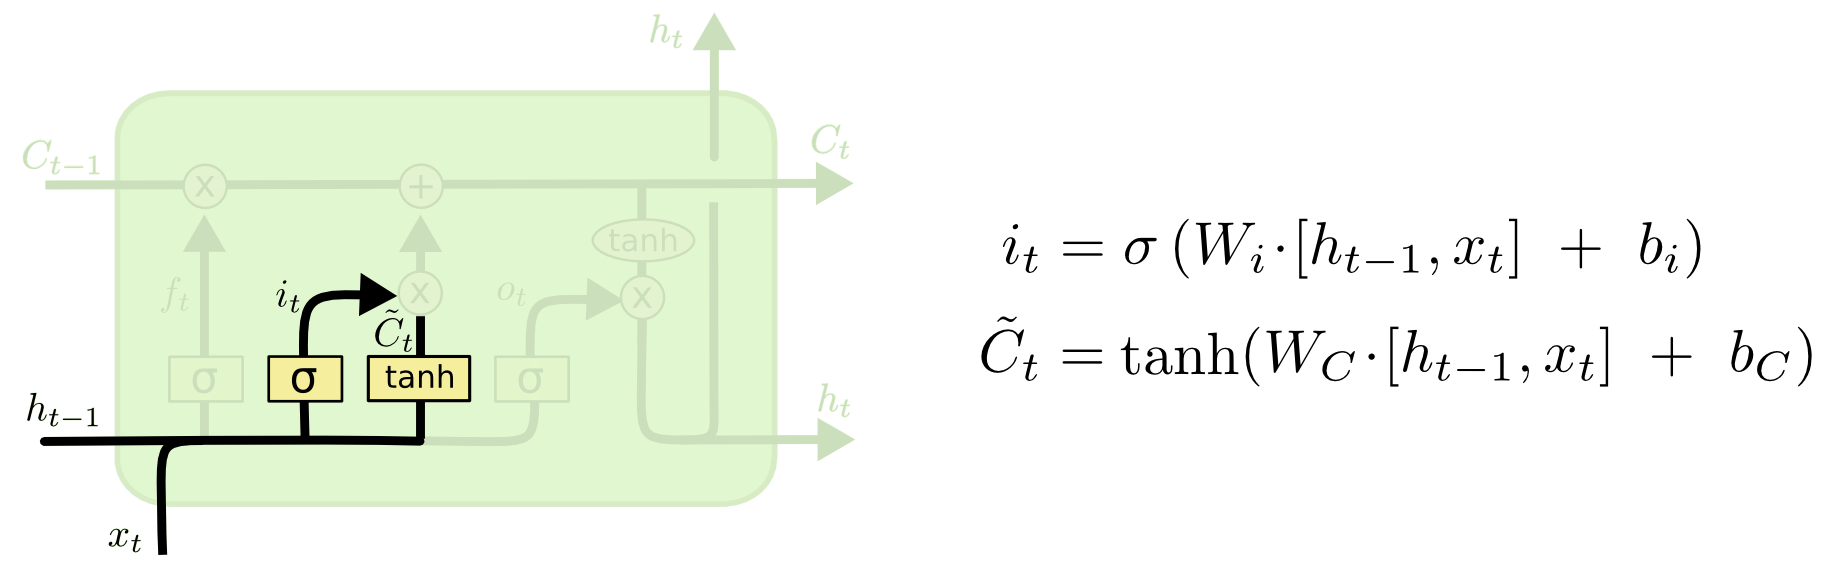
\includegraphics[scale=0.5]{LSTM3-focus-i.png}
\end{figure}
最后我们需要决定我们输出什么,输出取决于我们的cell state,但是将被过滤,所限我们运行sigmoid layer决定我们将输出那一部分。然后我们放通过tanh将cell state映射到-1,1,然后乘上sigmoid门的输出,以至于我们仅仅输出我们决定输出的部分。\par
对于语言模型的例子,因为它仅仅看subject,它也许想输出关于动词的信息,例子中的下一个,例如,它也许输出是否subject是单数或者复数,以至于从一个动词应该能知道接下来应该是动词的什么形式。
\begin{figure}
\centering
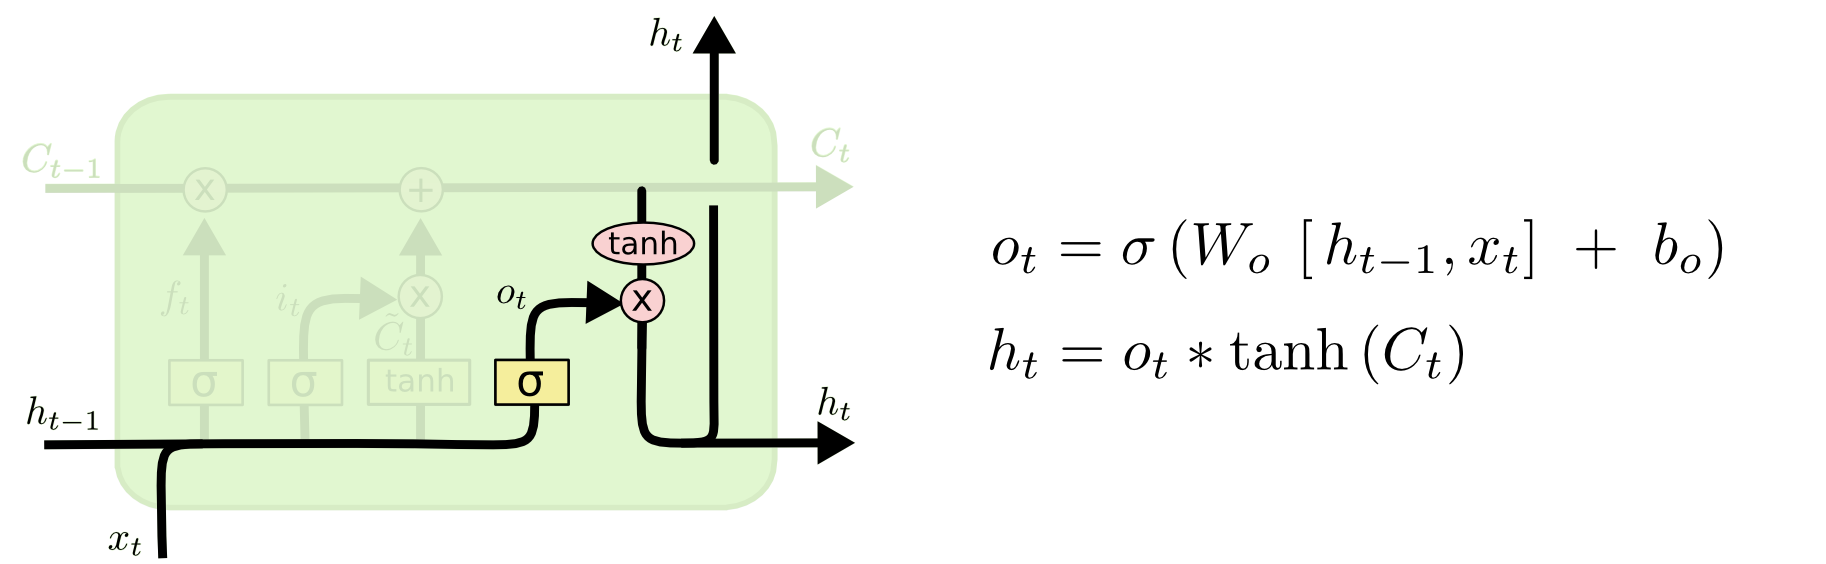
\includegraphics[scale=0.5]{LSTM3-focus-o.png}
\end{figure}
\subsection{LSTM的多种变体}
\href{ftp://ftp.idsia.ch/pub/juergen/TimeCount-IJCNN2000.pdf}{Gers  Schmidhuber (2000)},它增加了peephole connections,这一位置我们让gate layer通过cell state
\begin{figure}
\centering
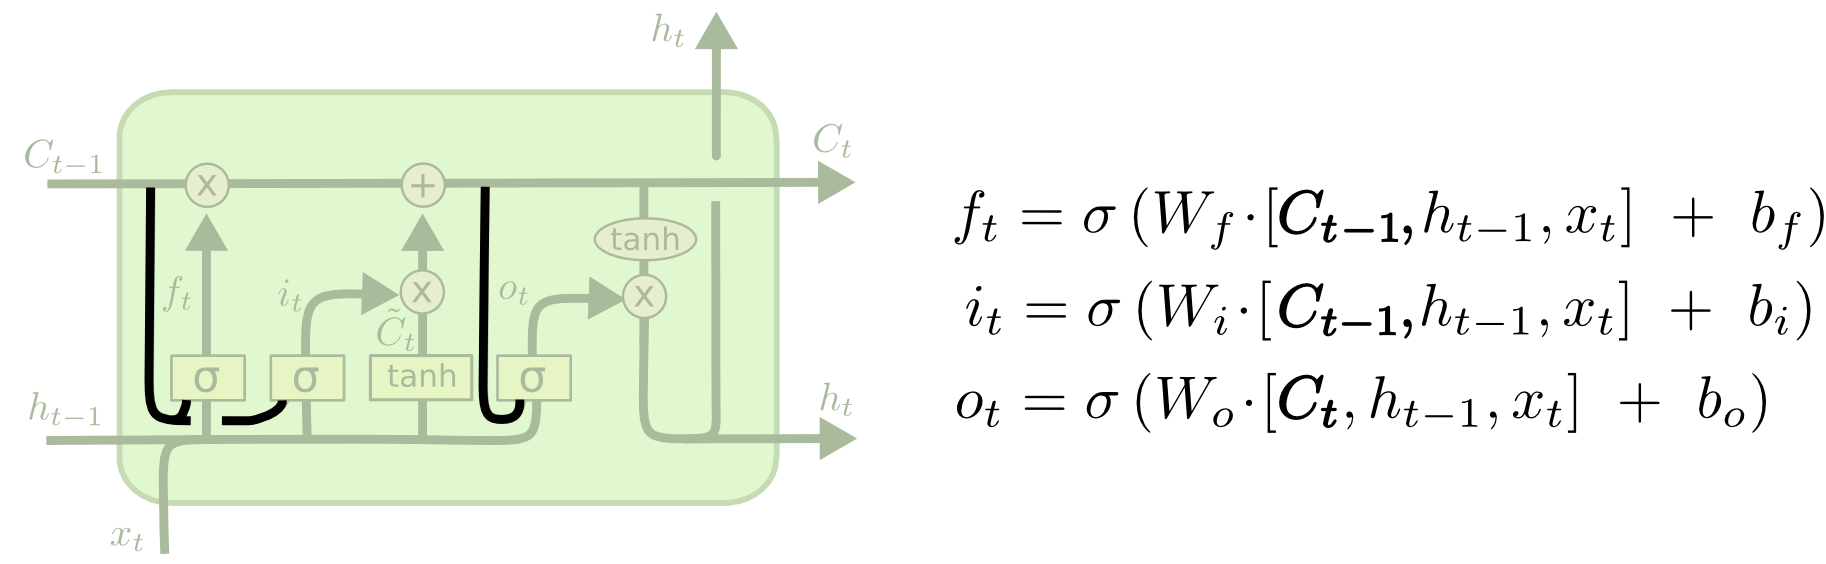
\includegraphics[scale=0.5]{LSTM3-var-peepholes.png}
\end{figure}
上面的图增加了peepholes到所有的门,但是一些论文给出一些peepholes和not others。另一个变体用两个forget 和输入门。而不是分别决定忘记或者添加信息,我们一起决定,我们需要输入一些值是忘记,我们仅仅忘记老的值输入新值到state
\begin{figure}
\centering
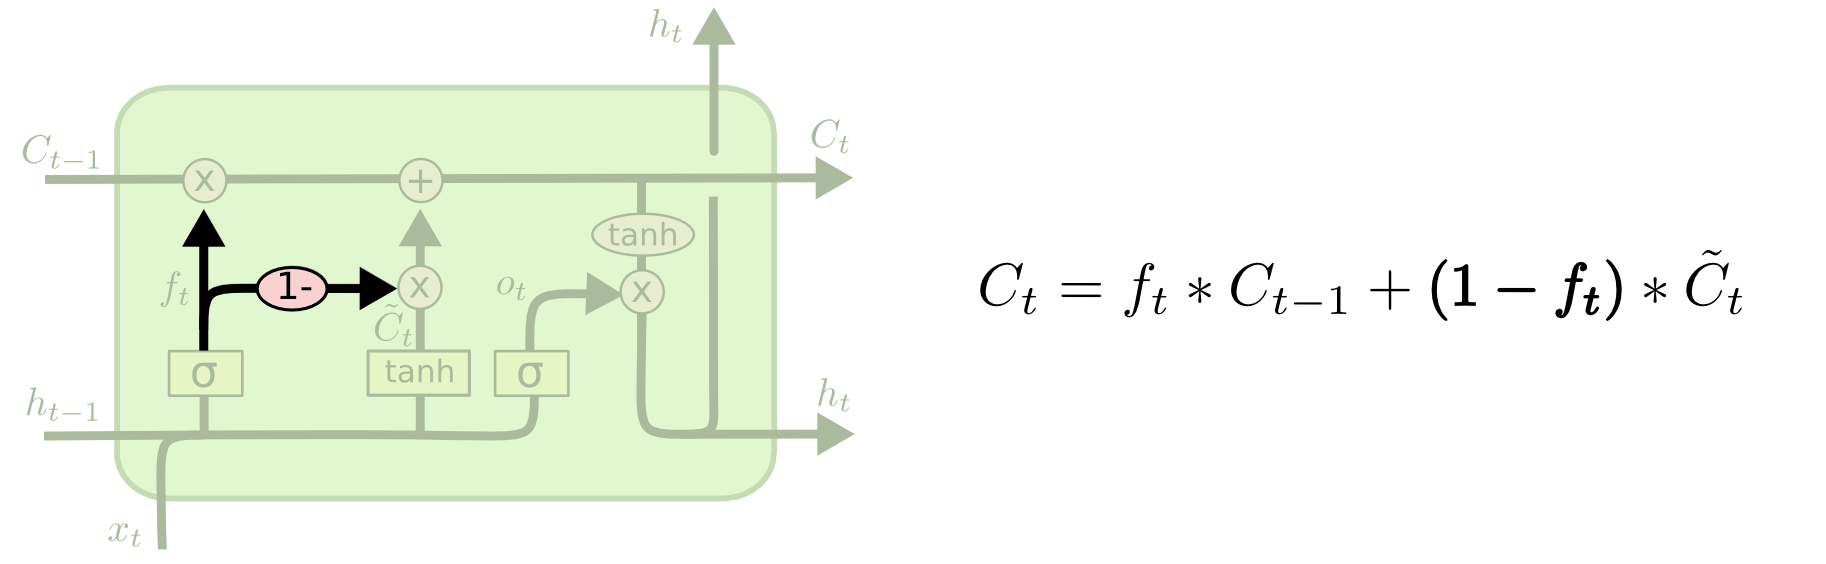
\includegraphics[scale=0.5]{LSTM3-var-tied.png}
\end{figure}
一个更引人注目的变体是Gate Recurrent Unit或者称为(GRU),由\href{http://arxiv.org/pdf/1406.1078v3.pdf}{Cho, et al. (2014)}引入,它结合忘记和输入门为一个单独的更新们,它也融合cell state和hidden state做了些改变,这结果模型比标准的LSTM模型简单,现在也越来越流行。
\begin{figure}
\centering
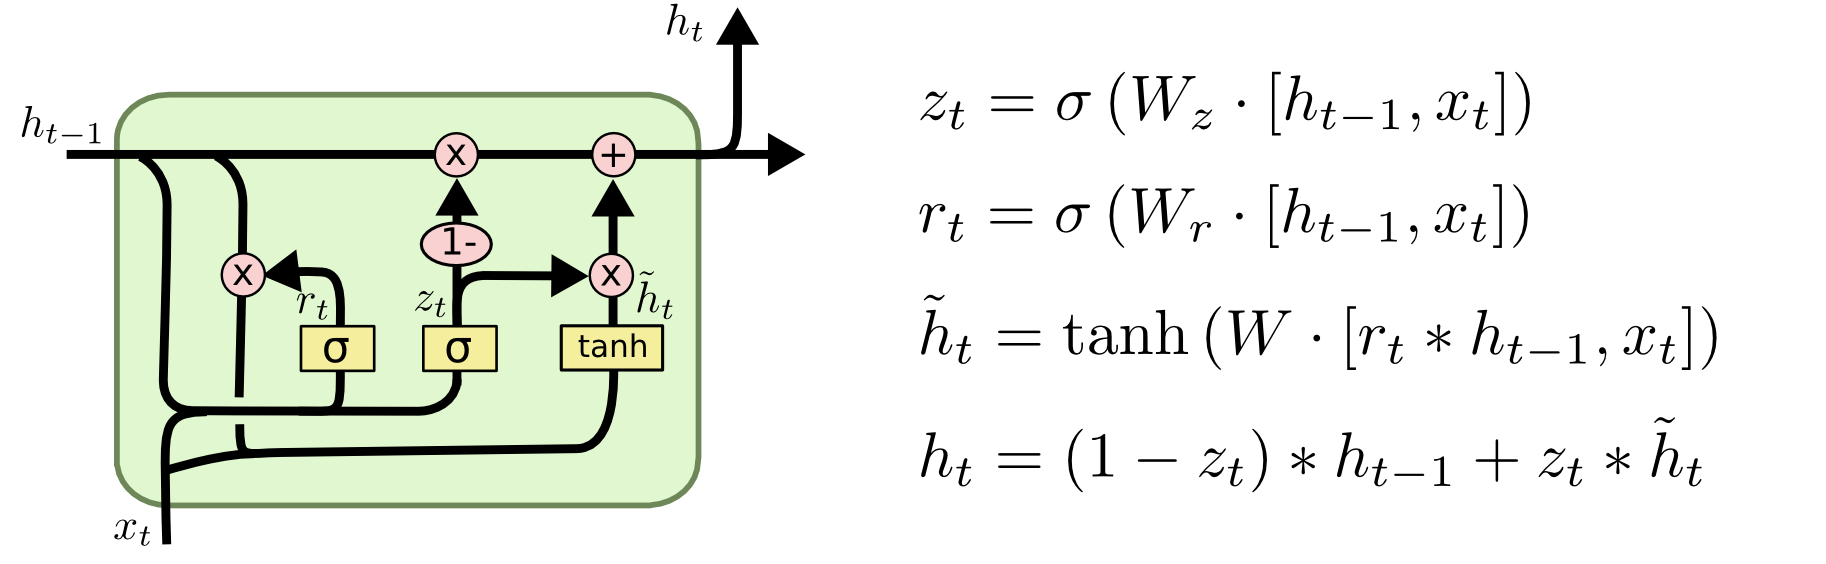
\includegraphics[scale=0.5]{LSTM3-var-GRU.png}
\end{figure}
这些仅仅是非常流行的LSTM变体,有一些其它的像\href{http://arxiv.org/pdf/1508.03790v2.pdf}{Yao, et al. (2015)}的Depth Gated RNNs,用完全不同的方法处理long-term dependencies,像\href{http://arxiv.org/pdf/1402.3511v1.pdf}{Koutnik, et al. (2014)}的Clockwork RNNs。\par
那个算法是最好的?他们的差别大吗?\href{http://arxiv.org/pdf/1503.04069.pdf}{Greff, et al. (2015) }做了一些比较了一些流行的变体,发现他们基本相同。
\href{http://jmlr.org/proceedings/papers/v37/jozefowicz15.pdf}{Jozefowicz, et al. (2015)}比较了超过1万中架构,找到了一些在确定问题上比LSTMs好的架构。
\subsection{向量字表示}
\subsubsection{Vector Representation of Words}
通常图像或音频系统处理的是由图片中所有单个原始像素点强度值或者音频中功率谱密度的强度值,把它们编码成丰富、高维度的向量数据集。对于物体或语音识别这一类的任务,我们所需的全部信息已经都存储在原始数据中(显然人类本身就是依赖原始数据进行日常的物体或语音识别的)。然后,自然语言处理系统通常将词汇作为离散的单一符号,例如 "cat" 一词或可表示为 Id537 ,而 "dog" 一词或可表示为 Id143。这些符号编码毫无规律,无法提供不同词汇之间可能存在的关联信息。换句话说,在处理关于 "dogs" 一词的信息时,模型将无法利用已知的关于 "cats" 的信息(例如,它们都是动物,有四条腿,可作为宠物等等)。可见,将词汇表达为上述的独立离散符号将进一步导致数据稀疏,使我们在训练统计模型时不得不寻求更多的数据。而词汇的向量表示将克服上述的难题。向量空间模型 (VSMs)将词汇表达(嵌套)于一个连续的向量空间中,语义近似的词汇被映射为相邻的数据点。向量空间模型在自然语言处理领域中有着漫长且丰富的历史,不过几乎所有利用这一模型的方法都依赖于 分布式假设,其核心思想为出现于上下文情景中的词汇都有相类似的语义。采用这一假设的研究方法大致分为以下两类:基于计数的方法 (e.g. 潜在语义分析), 和 预测方法 (e.g. 神经概率化语言模型).

其中它们的区别在如下论文中又详细阐述 \href{http://clic.cimec.unitn.it/marco/publications/acl2014/baroni-etal-countpredict-acl2014.pdf}{Baroni :et al},不过简而言之:基于计数的方法计算某词汇与其邻近词汇在一个大型语料库中共同出现的频率及其它统计量,然后将这些统计量映射到一个小型且稠密的向量中。预测方法则试图直接从某词汇的邻近词汇对其进行预测,在此过程中利用已经学习到的小型且稠密的嵌套向量。

Word2vec是一种可以进行高效率词嵌套学习的预测模型。其两种变体分别为:连续词袋模型(CBOW)及Skip-Gram模型。从算法角度看,这两种方法非常相似,其区别为CBOW根据源词上下文词汇('the cat sits on the')来预测目标词汇(例如,‘mat’),而Skip-Gram模型做法相反,它通过目标词汇来预测源词汇。Skip-Gram模型采取CBOW的逆过程的动机在于:CBOW算法对于很多分布式信息进行了平滑处理(例如将一整段上下文信息视为一个单一观察量)。很多情况下,对于小型的数据集,这一处理是有帮助的。相形之下,Skip-Gram模型将每个“上下文-目标词汇”的组合视为一个新观察量,这种做法在大型数据集中会更为有效。本教程余下部分将着重讲解Skip-Gram模型。
\subsubsection{处理噪声的对比训练}
神经概率化语言模型通常使用极大似然法 (ML) 进行训练,其中通过 softmax function 来最大化当提供前一个单词 h (代表 "history"),后一个单词的概率$w_t$(目标词概率)
\begin{equation*}
P(w_t|h)=softmax(score(w_t,h))=\frac{exp\left\{score(w_t,h)\right\}}{\Sigma_{Word w' in Vocab}exp\left\{score(w',h)\right\}}
\end{equation*}
当 $score(w_t,h)$ 计算了文字 $w_t$ 和 上下文 h 的相容性(通常使用向量积)。我们使用对数似然函数来训练训练集的最大值,比如通过:
\begin{equation*}
J_{ML} = logP(w_t|h)=score(w_t,h)-log(\Sigma_{Word w' in Vocab}exp\left\{score(w',h)\right\})
\end{equation*}
这里提出了一个解决语言概率模型的合适的通用方法。然而这个方法实际执行起来开销非常大,因为我们需要去计算并正则化当前上下文环境 h 中所有其它 V 单词 w' 的概率得分,在每一步训练迭代中。
\begin{figure}[H]
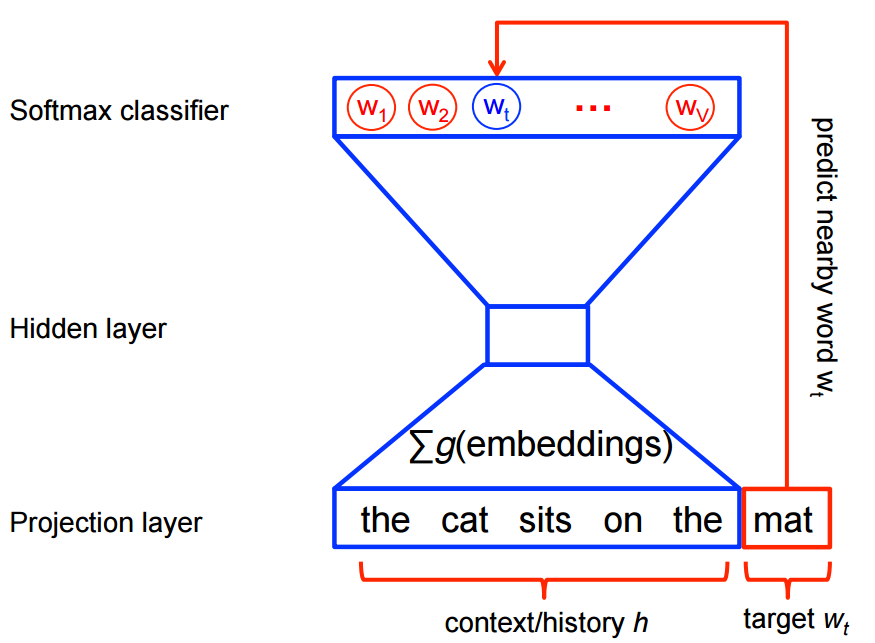
\includegraphics[scale=0.5]{softmax-nplm.png}
\caption{CBOW方法}
\end{figure}
从另一个角度来说,当使用word2vec模型时,我们并不需要对概率模型中的所有特征进行学习。而CBOW模型和Skip-Gram模型为了避免这种情况发生,使用一个二分类器(逻辑回归)在同一个上下文环境里从 k 虚构的 (噪声) 单词$\hat{w}$区分真正的目标单词$w_t$,下面详细参数CBOW模型,对于Skip-Gram模型只要简单的反向操作即可。
\begin{center}
\begin{figure}[H]
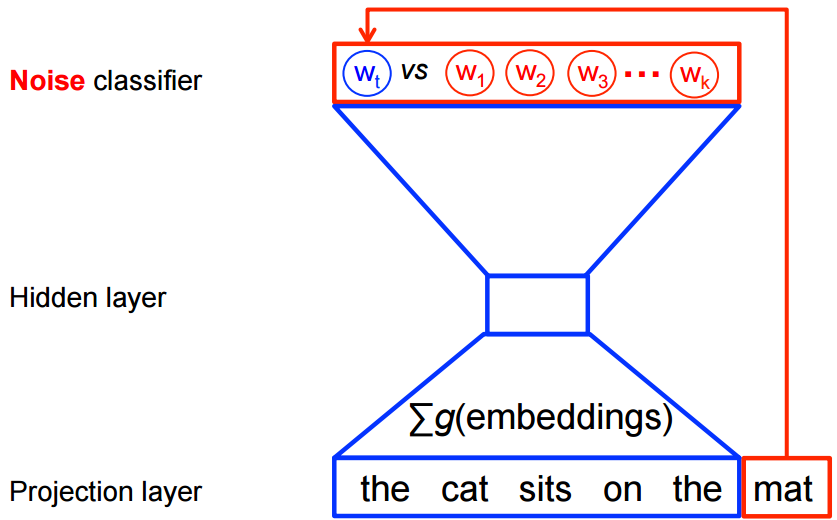
\includegraphics[scale=0.5]{nce-nplm.png}
\caption{Skip-Gram}
\end{figure}
\end{center}
从数学的角度来说,我们的目标是对每个样本最大化:
\begin{equation*}
J_{NEG}=logQ_{\theta}(D=1|w_t,h)+k\underset{\hat{w}\sim P_{noise}}{E}[logQ_{\theta}(D=0|\hat{\omega},h)]
\end{equation*}
其中$Q_{\theta}(D=1|w,h)$代表的是当前上下文h,根据所学得嵌套向量$\theta$目标单词 w 使用二分类逻辑回归计算得出的概率。在实践中,我们通过在噪声分布中绘制比对文字来获得近似的期望值(通过计算\href{https://en.wikipedia.org/wiki/Monte_Carlo_integration}{蒙特卡洛平均值})。

当真实地目标单词被分配到较高的概率,同时噪声单词的概率很低时,目标函数也就达到最大值了。从技术层面来说,这种方法叫做\href{http://papers.nips.cc/paper/5021-distributed-representations-of-words-and-phrases-and-their-compositionality.pdf}{负抽样},而且使用这个损失函数在数学层面上也有很好的解释:这个更新过程也近似于softmax函数的更新。这在计算上将会有很大的优势,因为当计算这个损失函数时,只是有我们挑选出来的 k 个 噪声单词,而没有使用整个语料库 V。这使得训练变得非常快。我们实际上使用了与\href{http://papers.nips.cc/paper/5165-learning-word-embeddings-efficiently-with-noise-contrastive-estimation.pdf}{noise-contrastive estimation (NCE)}介绍的非常相似的方法,这在TensorFlow中已经封装了一个很便捷的函数tf.nn.nce\_loss()。

\subsubsection{Skip-gram模型}
下面来看一下这个数据集

the quick brown fox jumped over the lazy dog

我们首先对一些单词以及它们的上下文环境建立一个数据集。我们可以以任何合理的方式定义‘上下文’,而通常上这个方式是根据文字的句法语境的(使用语法原理的方式处理当前目标单词可以看一下这篇文献 \href{https://levyomer.files.wordpress.com/2014/04/dependency-based-word-embeddings-acl-2014.pdf}{Levy et al.},比如说把目标单词左边的内容当做一个‘上下文’,或者以目标单词右边的内容,等等。现在我们把目标单词的左右单词视作一个上下文, 使用大小为1的窗口,这样就得到这样一个由(上下文, 目标单词) 组成的数据集:

([the, brown], quick), ([quick, fox], brown), ([brown, jumped], fox), ...

前文提到Skip-Gram模型是把目标单词和上下文颠倒过来,所以在这个问题中,举个例子,就是用'quick'来预测 'the' 和 'brown' ,用 'brown' 预测 'quick' 和 'fox' 。因此这个数据集就变成由(输入, 输出)组成的:

(quick, the), (quick, brown), (brown, quick), (brown, fox), ...

目标函数通常是对整个数据集建立的,但是本问题中要对每一个样本(或者是一个batch\_size 很小的样本集,通常设置为16 <= batch\_size <= 512)在同一时间执行特别的操作,称之为\href{https://en.wikipedia.org/wiki/Stochastic_gradient_descent}{随机梯度下降 (SGD)}。我们来看一下训练过程中每一步的执行。

假设用 t 表示上面这个例子中quick 来预测 the 的训练的单个循环。用 num\_noise 定义从噪声分布中挑选出来的噪声(相反的)单词的个数,通常使用一元分布,P(w)。为了简单起见,我们就定num\_noise=1,用 sheep 选作噪声词。接下来就可以计算每一对观察值和噪声值的损失函数了,每一个执行步骤就可表示为:
\begin{equation*}
J_{NEG}^{(t)}=logQ_{\theta}(D=1|the,quick)+log(Q_{\theta}(D=0|sleep,quick))
\end{equation*}
整个计算过程的目标是通过更新嵌套参数$\theta$来逼近目标函数(这个例子中就是使目标函数最大化)。为此我们要计算损失函数中嵌套参数$\theta$的梯度,比如\[\frac{\partial}{\partial}J_{NEG}\]
(幸好TensorFlow封装了工具函数可以简单调用!)。对于整个数据集,当梯度下降的过程中不断地更新参数,对应产生的效果就是不断地移动每个单词的嵌套向量,直到可以把真实单词和噪声单词很好得区分开。

我们可以把学习向量映射到2维中以便我们观察,其中用到的技术可以参考 \href{http://lvdmaaten.github.io/tsne/}{t-SNE 降维技术}。当我们用可视化的方式来观察这些向量,就可以很明显的获取单词之间语义信息的关系,这实际上是非常有用的。当我们第一次发现这样的诱导向量空间中,展示了一些特定的语义关系,这是非常有趣的,比如文字中 male-female,gender 甚至还有 country-capital 的关系, 如下方的图所示 (也可以参考 \href{http://www.aclweb.org/anthology/N13-1090}{Mikolov et al.}, 2013论文中的例子)。
\begin{center}
\begin{figure}[H]
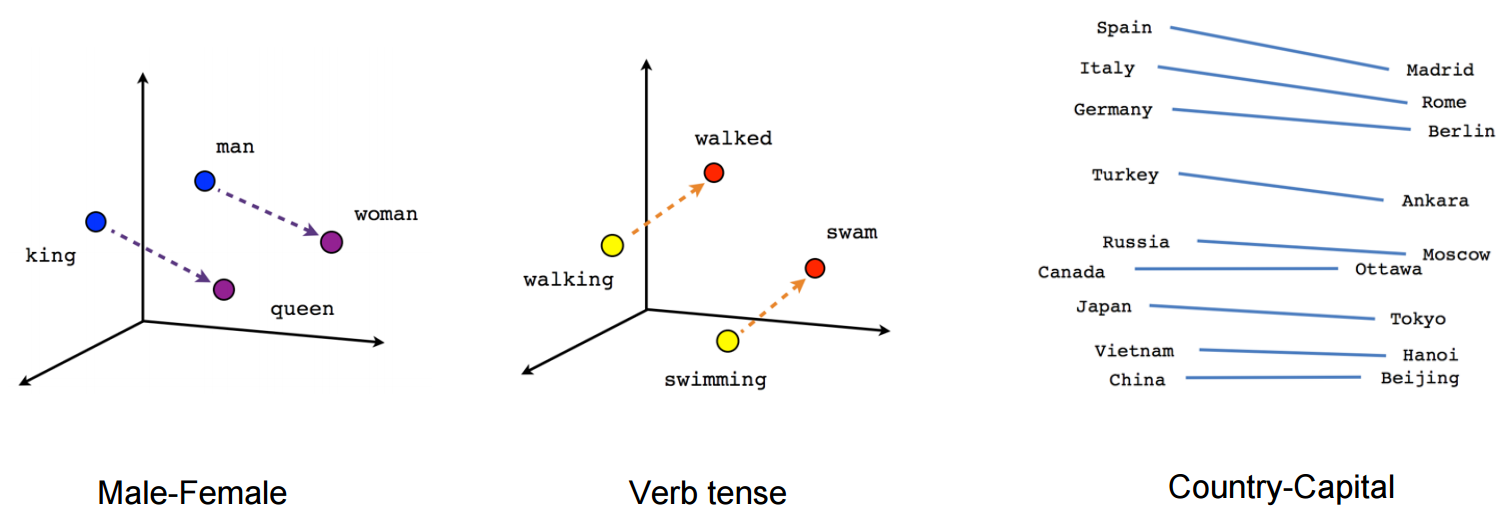
\includegraphics[scale=0.5]{linear-relationships.png}
\end{figure}
\end{center}
这也解释了为什么这些向量在传统的NLP问题中可作为特性使用,比如用在对一个演讲章节打个标签,或者对一个专有名词的识别 (看看如下这个例子 \href{https://arxiv.org/pdf/1103.0398v1.pdf}{Collobert et al.}或者 \href{http://www.aclweb.org/anthology/P10-1040}{Turian et al.})。

不过现在让我们用它们来画漂亮的图表吧!

这里谈得都是嵌套,那么先来定义一个嵌套参数矩阵。我们用唯一的随机值来初始化这个大矩阵。
\begin{python}
embeddings = tf.Variable(
    tf.random_uniform([vocabulary_size, embedding_size], -1.0, 1.0))
\end{python}
对噪声-比对的损失计算就使用一个逻辑回归模型。对此,我们需要对语料库中的每个单词定义一个权重值和偏差值。(也可称之为输出权重 与之对应的 输入嵌套值)。定义如下:
\begin{python}
nce_weights = tf.Variable(
  tf.truncated_normal([vocabulary_size, embedding_size],
                      stddev=1.0 / math.sqrt(embedding_size)))
nce_biases = tf.Variable(tf.zeros([vocabulary_size]))
\end{python}我们有了这些参数之后,就可以定义Skip-Gram模型了。简单起见,假设我们已经把语料库中的文字整型化了,这样每个整型代表一个单词(细节请查看\_basic.py)。Skip-Gram模型有两个输入。一个是一组用整型表示的上下文单词,另一个是目标单词。给这些输入建立占位符节点,之后就可以填入数据了。
\begin{python}
train_inputs = tf.placeholder(tf.int32, shape=[batch_size])
train_labels = tf.placeholder(tf.int32, shape=[batch_size, 1])
\end{python}
然后我们需要对批数据中的单词建立嵌套向量,TensorFlow提供了方便的工具函数。
\begin{python}
embed = tf.nn.embedding_lookup(embeddings, train_inputs)
\end{python}
好了,现在我们有了每个单词的嵌套向量,接下来就是使用噪声-比对的训练方式来预测目标单词。
\begin{python}
loss = tf.reduce_mean(
  tf.nn.nce_loss(nce_weights, nce_biases, embed, train_labels,
                 num_sampled, vocabulary_size))
\end{python}
我们对损失函数建立了图形节点,然后我们需要计算相应梯度和更新参数的节点,比如说在这里我们会使用随机梯度下降法,TensorFlow也已经封装好了该过程。
\begin{python}
optimizer = tf.train.GradientDescentOptimizer(learning_rate=1.0).minimize(loss)
\end{python}
\subsubsection{训练过程}
训练的过程很简单,只要在循环中使用feed\_dict不断给占位符填充数据,同时调用 session.run即可。
\begin{python}
for inputs, labels in generate_batch(...):
  feed_dict = {training_inputs: inputs, training_labels: labels}
  _, cur_loss = session.run([optimizer, loss], feed_dict=feed_dict)
\end{python}
\subsubsection{嵌套学习结果可视化}
\begin{center}
\begin{figure}[H]
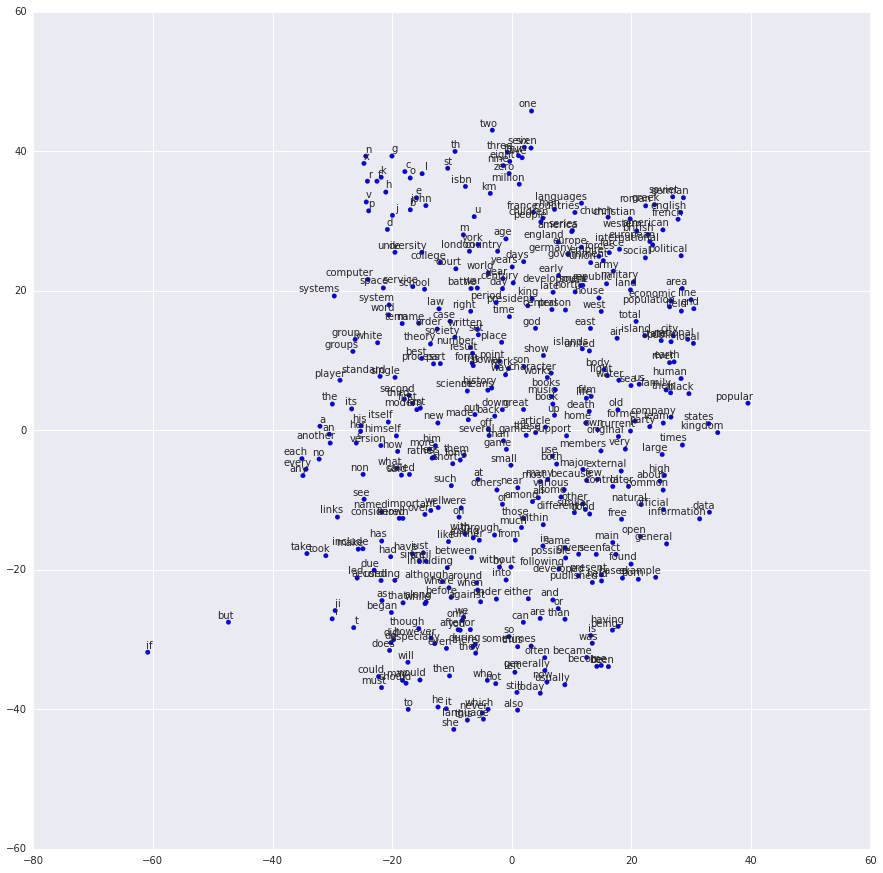
\includegraphics[scale=0.5]{tsne.png}
\end{figure}
\end{center}
Et voila! 与预期的一样,相似的单词被聚类在一起。对word2vec模型更复杂的实现需要用到TensorFlow一些更高级的特性,具体是实现可以参考\href{https://github.com/bleedingfight/models/tree/master/tutorials/embedding}{word2vec.py}\subsubsection{嵌套学习的评估:类比推理}
词嵌套在NLP的预测问题中是非常有用且使用广泛地。如果要检测一个模型是否是可以成熟地区分词性或者区分专有名词的模型,最简单的办法就是直接检验它的预测词性、语义关系的能力,比如让它解决形如king is to queen as father is to ?这样的问题。这种方法叫做类比推理 ,可参考Mikolov and colleagues,数据集下载地址为:\href{https://word2vec.googlecode.com/svn/trunk/questions-words.txt}{questions-words.txt} 。
To see how we do this evaluation如何执行这样的评估,可以看build\_eval\_graph()和 eval()这两个函数在下面源码中的使用 \href{https://github.com/bleedingfight/models/tree/master/tutorials/embedding}{word2vec.py}

超参数的选择对该问题解决的准确性有巨大的影响。想要模型具有很好的表现,需要有一个巨大的训练数据集,同时仔细调整参数的选择并且使用例如二次抽样的一些技巧。不过这些问题已经超出了本教程的范围。
\subsubsection{优化实现}
以上简单的例子展示了TensorFlow的灵活性。比如说,我们可以很轻松得用现成的tf.nn.sampled\_softmax\_loss()来代替tf.nn.nce\_loss()构成目标函数。如果你对损失函数想做新的尝试,你可以用TensorFlow手动编写新的目标函数的表达式,然后用控制器执行计算。这种灵活性的价值体现在,当我们探索一个机器学习模型时,我们可以很快地遍历这些尝试,从中选出最优。

一旦你有了一个满意的模型结构,或许它就可以使实现运行地更高效(在短时间内覆盖更多的数据)。比如说,在本教程中使用的简单代码,实际运行速度都不错,因为我们使用Python来读取和填装数据,而这些在TensorFlow后台只需执行非常少的工作。如果你发现你的模型在输入数据时存在严重的瓶颈,你可以根据自己的实际问题自行实现一个数据阅读器,参考 新的数据格式。对于Skip-Gram 模型,我们已经完成了如下这个例子 \href{https://github.com/bleedingfight/models/tree/master/tutorials/embedding}{word2vec.py}。

如果I/O问题对你的模型已经不再是个问题,并且想进一步地优化性能,或许你可以自行编写TensorFlow操作单元,详见 添加一个新的操作。相应的,我们也提供了Skip-Gram模型的例子 \href{https://github.com/bleedingfight/models/tree/master/tutorials/embedding}{optimized.py}。请自行调节以上几个过程的标准,使模型在每个运行阶段有更好地性能。
\subsection{RNN}
此教程将展示如何在高难度的语言模型中训练循环神经网络。该问题的目标是获得一个能确定语句概率的概率模型。为了做到这一点,通过之前已经给出的词语来预测后面的词语。我们将使用 PTB(Penn Tree Bank) 数据集,这是一种常用来衡量模型的基准,同时它比较小而且训练起来相对快速。

语言模型是很多有趣难题的关键所在,比如语音识别,机器翻译,图像字幕等。它很有意思--可以参看 here。

本教程的目的是重现 \href{http://arxiv.org/abs/1409.2329}{Zaremba et al., 2014} 的成果,他们在 PTB 数据集上得到了很棒的结果。
\subsubsection{下载及准备数据}
本教程需要的数据在 data/ 路径下,来源于 Tomas Mikolov 网站上的\href{http://www.fit.vutbr.cz/~imikolov/rnnlm/simple-examples.tg}{PTB 数据集}

该数据集已经预先处理过并且包含了全部的 10000 个不同的词语,其中包括语句结束标记符,以及标记稀有词语的特殊符号 (<unk>) 。我们在 reader.py 中转换所有的词语,让他们各自有唯一的整型标识符,便于神经网络处理。
\subsubsection{LSTM}
模型的核心由一个 LSTM 单元组成,其可以在某时刻处理一个词语,以及计算语句可能的延续性的概率。网络的存储状态由一个零矢量初始化并在读取每一个词语后更新。而且,由于计算上的原因,我们将以 batch\_size 为最小批量来处理数据。

基础的伪代码就像下面这样:
\begin{python}
lstm = rnn_cell.BasicLSTMCell(lstm_size)
state = tf.zeros([batch_size, lstm.state_size])

loss = 0.0
for current_batch_of_words in words_in_dataset:
    output, state = lstm(current_batch_of_words, state)

    logits = tf.matmul(output, softmax_w) + softmax_b
    probabilities = tf.nn.softmax(logits)
    loss += loss_function(probabilities, target_words)
\end{python}
\subsubsection{截断反向传播}
为使学习过程易于处理,通常的做法是将反向传播的梯度在(按时间)展开的步骤上照一个固定长度(num\_steps)截断。 通过在一次迭代中的每个时刻上提供长度为 num\_steps 的输入和每次迭代完成之后反向传导,这会很容易实现。

一个简化版的用于计算图创建的截断反向传播代码:
\begin{python}
words = tf.placeholder(tf.int32, [batch_size, num_steps])

lstm = rnn_cell.BasicLSTMCell(lstm_size)
initial_state = state = tf.zeros([batch_size, lstm.state_size])

for i in range(len(num_steps)):
    output, state = lstm(words[:, i], state)

    # ...

final_state = state
\end{python}
下面展现如何实现迭代整个数据集:
\begin{python}
numpy_state = initial_state.eval()
total_loss = 0.0
for current_batch_of_words in words_in_dataset:
    numpy_state, current_loss = session.run([final_state, loss],
        feed_dict={initial_state: numpy_state, words: current_batch_of_words})
    total_loss += current_loss
\end{python}
\subsubsection{输入}
在输入 LSTM 前,词语 ID 被嵌入到了一个密集的表示中(查看 矢量表示教程)。这种方式允许模型高效地表示词语,也便于写代码:
\begin{python}
# embedding_matrix 张量的形状是: [vocabulary_size, embedding_size]
word_embeddings = tf.nn.embedding_lookup(embedding_matrix, word_ids)
\end{python}
嵌入的矩阵会被随机地初始化,模型会学会通过数据分辨不同词语的意思。
\subsubsection{损失函数}
我们想使目标词语的平均负对数概率最小$loss = -\frac{1}{N}\Sigma_{i=1}^NlnP_{target_i}$
实现起来并非很难,而且函数 sequence\_loss\_by\_example 已经有了,可以直接使用。

论文中的典型衡量标准是每个词语的平均困惑度(perplexity),计算式为
$$e^{-\frac{1}{N}\Sigma_{i=1}^N}lnp_{target_i}=e^{loss}$$
同时我们会观察训练过程中的困惑度值(perplexity)
\subsubsection{多个LSTM层堆叠}
要想给模型更强的表达能力,可以添加多层 LSTM 来处理数据。第一层的输出作为第二层的输入,以此类推。

类 MultiRNNCell 可以无缝的将其实现:
\begin{python}
lstm = rnn_cell.BasicLSTMCell(lstm_size)
stacked_lstm = rnn_cell.MultiRNNCell([lstm] * number_of_layers)

initial_state = state = stacked_lstm.zero_state(batch_size, tf.float32)
for i in range(len(num_steps)):
    # 每次处理一批词语后更新状态值.
    output, state = stacked_lstm(words[:, i], state)

    # 其余的代码.
    # ...

final_state = state
\end{python}
\subsubsection{编译并运行代码}
首先需要构建库,在CPU上编译:
\begin{python}
bazel build -c opt tensorflow/models/rnn/ptb:ptb_word_lm
\end{python}
如果你有一个强大的 GPU,可以运行
\begin{python}
bazel build -c opt --config=cuda tensorflow/models/rnn/ptb:ptb_word_lm
\end{python}
运行模型:
\begin{python}
bazel-bin/tensorflow/models/rnn/ptb/ptb_word_lm \
  --data_path=/tmp/simple-examples/data/ --alsologtostderr --model small
\end{python}
教程代码中有 3 个支持的模型配置参数:"small", "medium" 和 "large"。它们指的是 LSTM 的大小,以及用于训练的超参数集。

模型越大,得到的结果应该更好。在测试集中 small 模型应该可以达到低于 120 的困惑度(perplexity),large 模型则是低于 80,但它可能花费数小时来训练。

\chapter{Tensorflow进阶}
\section{模型存储和加载}
\begin{itemize}
\item 生成checkpoint文件,扩展名一般为.ckpt,通过在tf.train.Saver对象上调用Saver.saver()生成。它包含权重和其他程序中定义的变量,不包含
图的结构。如果需要在另一个程序中使用,需要重建图形结构,并告诉Tensorflow如何处理这些权重。
\item 生成(graph proto file),这是一个二进制文件,扩展名一般是.pb,用tf.train.write\_graph()保存每,只包含图形结构,不包含权重,然后使用tf.import\_graph\_def()加载
图形。
\end{itemize}


\section{用GPU}
在Tensorflow中CPU,GPU用字符串表示
\begin{itemize}
\item "cpu:0":机器上的CPU
\item "gpu:0":机器上的GPU
\item "gpu:1":机器上的第二块GPU
\end{itemize}
 如果TensorFLow操作有GPU和CPU实现,GPU将被优先指定,例如matmul有CPU和GPU内核,在系统上 有cpu:0和gpu:0,gpu:0将优先运行matmul。
布置采集设备

找到你的操作和tensor上的设备,创建一个会话log\_device\_placement配置设置为True
\begin{python}
import tensorflow as tf
a = tf.reshape(tf.linspace(-1.,1.,12),(3,4))
b = tf.reshape(tf.sin(a),(4,3))
c = tf.matmul(a,b)
with tf.Session() as sess:
    print(sess.run(c))
\end{python}
输出参数:\newline
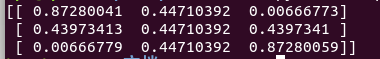
\includegraphics{./pic/chapter2/use_gpu1.png}\newline
\subsection{手工配置设备}
如果你想将你的操作运行在指定的设备中而不由tensorflow是自动为你选择,你可以用tf.device 创建一个设备,左右的操作将在同一个设备上指定。
\begin{python}
import tensorflow as tf
with tf.device('/cpu:0'):
    a = tf.constant([1.,2.,3.,4.,5.,6.],shape = (2,3),name = 'a')
    b = tf.reshape(a,shape=(3,2))
    c = tf.matmul(a,b)
    with tf.Session(config = tf.ConfigProto(log_device_placement=True)) as sess:
        print(sess.run(c))
\end{python}
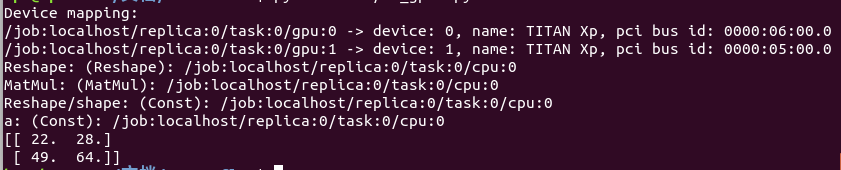
\includegraphics[scale=0.4]{use_gpu2.png}\newline
正如你看到的a,b被复制到cpu:0,因为设备没有明确指定,Tensorflow将选择操作和可用的设备(gpu:0)

\subsection{允许GPU的内存增长}

默认情况下Tensorflow将映射所有的CPUs的显存到进程上,用相对精确的GPU内存资源减少内存的碎片化会更高效。 通常有些程序希望分贝可用内存的一部分,或者增加内存的需要两。在会话中tensorflow提供了两个参数 控制它。 第一个参数是allow\_growth选项,根据运行情况分配GPU内存:它开始分配很少的内存,当Session开始运行 需要更多GPU内存是,我们同感Tensorflow程序扩展GPU的内存区域。注意我们不释放内存,因此这可能导致更多的内存碎片。为了开启这个选项,可以通过下面的设置
\begin{python}
config = tf.ConfigProto()
config.gpu_option.allow_growth = True
sess = tf.Session(config=config,...)
\end{python}
第二种方法是per\_process\_gpu\_memory\_fraction选项,决定GPU总体内存中多少应给被分配,例如你可以告诉 Tensorflow分配40\%的GPU总体内存。
\begin{python}
config = tf.ConfigProto()
config.gpu_option.per_process_gpu_memory_fraction = 0.4
sess = tf.Session(config = config)
\end{python}
如果你想限制Tensorflow程序的GPU使用量,这个参数是很有用的。

在多GPU系统是使用GPU

如果你的系统上有超过一个GPU,你的GPU的抵消的ID将被默认选中,如果你想运行在不同的GPU上,你需要指定 你想要执行运算的GPU
\begin{python}
import tensorflow as tf
with tf.device('/gpu2:0'):
    a = tf.constant([1.,2.,3.,4.,5.,6.],shape = (2,3),name = 'a')
    b = tf.reshape(a,shape=(3,2))
    c = tf.matmul(a,b)
    with tf.Session(config = tf.ConfigProto(log_device_placement=True)) as sess:
        print(sess.run(c))
\end{python}
如果你指定的设备不存在,你将个到一个InvalidArgumentError:\newline
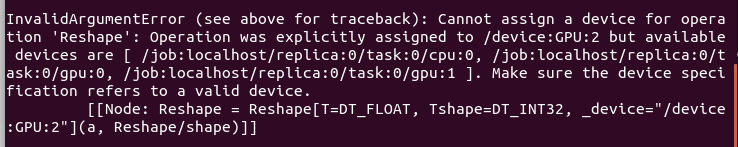
\includegraphics[scale=0.4]{use_gpu3.png}\newline
如果你想Tensorflow在万一指定的设备不存在时自动选择一个存在的设备,你可以在创建会话时配置中设置allow\_soft\_placement 为True
\begin{python}
with tf.device('/gpu:2'):
  a = tf.constant([1.,2.,3.,4.,5.,6.],shape= [3,2],name = 'a')
  b = tf.constant([1.,2.,3.,4.,5.,6.],shape= [2,3],name = 'b')
  c = tf.matmul(a,b)
with tf.Session(config = tf.ConfigProto(allow_soft_placement=True,log_device_placement=True)) as sess:
    print(sess.run(c))
\end{python}
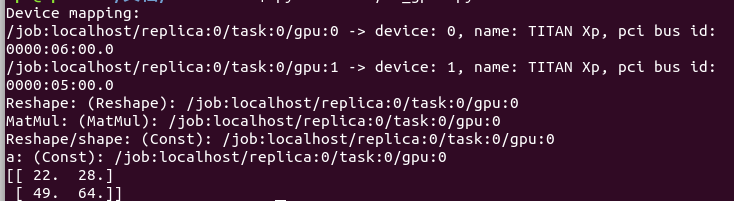
\includegraphics[scale=0.4]{use_gpu4.png}\newline
用多GPU

如果你想在多张GPU上运行Tensorflow,你可以在multi-tower fashion上构造你的模型,每个tower 被指定到不同的GPU上。例如:
\begin{python}
c = []
for d in ['/gpu:0', '/gpu:1']:
    with tf.device(d):
        a = tf.constant([1.0, 2.0, 3.0, 4.0, 5.0, 6.0], shape=[2, 3])
        b = tf.constant([1.0, 2.0, 3.0, 4.0, 5.0, 6.0], shape=[3, 2])
        c.append(tf.matmul(a, b))
    with tf.device('/cpu:0'):
        sum = tf.add_n(c)
   # Creates a session with log_device_placement set to True.
sess = tf.Session(config=tf.ConfigProto(allow_soft_placement=True,log_device_placement=True))
  # Runs the op.
print(sess.run(sum))
sess.close()
\end{python}
\section{如何利用Inception的最后一层重新训练新的分类}
现代的认知模型可能有上百万个参数可能需要花几周训练,Transfer学习是通过完整的像ImageNet一样的模型通过已经存在的权重简化数周工作分类的技术。在这个例子中我们将创新训练最终层不修改其它层。详细信息你可以查看\href{http://arxiv.org/pdf/1310.1531v1.pdf}{这篇论文}.

尽管不完整的训练,但是对于一些应用却惊人的高效,可以在笔记本上训练30分钟,不要求GPU。这个导航将显示给你如何在自己的图像运行示例脚本解释一些控制训练需要的脚本。
\subsection{训练花}
\begin{center}
\begin{figure}
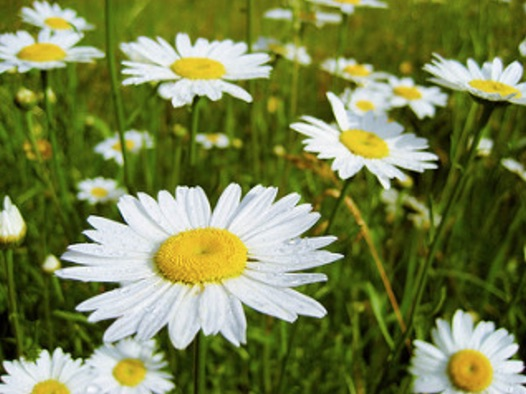
\includegraphics[scale=0.5]{daisies.jpg}
\end{figure}
\end{center}
在开始训练前你需要设置图像教网络你想认识的新的类别。接下来的张杰解释如何准备你的图像,但是我们创建一个授权的归档的花的文件使得训练更轻松。为了得到花的图像,运行下面的代码:
\begin{lstlisting}[language={[ANSI]C}]
cd ~
curl -O http://download.tensorflow.org/example_images/flower_photos.tgz
tar xzf flower_photos.tgz
\end{lstlisting}
当你有图像后,你从你的TensorFlow源文件目录构建重新训练器
\begin{lstlisting}[language={[ANSI]C}]
bazel build --config opt tensorflow/examples/image_retraining:retrain
\end{lstlisting}
可以通过下面运行:
\begin{lstlisting}{language=[ANSI]C}
bazel build tensorflow/examples/image_retraining:retrain
\end{lstlisting}
如果你有一个机器支持AVX设备集(最近几年的常用的x86 CPUs)你可以通过架构提高building运行速度
\begin{lstlisting}{language=[ANSI]C}
bazel build --config opt tensorflow/examples/image_retraining:retrain
\end{lstlisting}
训练器可以是这样:
\begin{lstlisting}{language=[ANSI]C}
bazel-bin/tensorflow/examples/image_retraining/retrain --image_dir ~/flower_photos
\end{lstlisting}
这个脚本载入先前incption v3模型,删除顶层,在新的flower photos训练新的模型。在原始ImageNet类中没有一种花完整网络被完整的训练过了,transfer学习是低层已经被训练好
区别不修改任何不同对象。
\subsection{瓶颈}
训练花费30分钟甚至更长时间取决于你的机器的速度。第一个时期分析所有磁盘上的图像和计算他们的瓶颈,瓶颈是一个信息对术语
我们经常在最后一层前一层,倒数第二层已经训练区别输出要求分类的值,这意味着这必须是有意义的,因此对于分类器它必须包含足够的信息在一些小的值得集合中做选择,这意味着我们的最终层训练可以在新的类中工作证明在ImageNet中1000类对于区别新的对象是有用的。
因为每个图像在训练和计算花费时间瓶颈时被多次使用,他的速度达到缓存起的瓶颈因此不能被重复计算。默认他们存储在/tmp/bottleneck陌路,如果你仍然会脚本他们将被重用,因此你不是必须再次等待这部分。
\subsection{训练}
当瓶颈计算完成时,实际顶层训练开始。你讲看到输出,显示精度,可用精度,交叉熵。训练精度显示在当前训练批中多少被分类正确,验证训练精度从图像数据集随机选中精度的值,不同之处在于训练精度基于网络已经学习到的参数,在训练中可能过拟合到为噪声。验证精确度用不在训练集中的数据性能测量精确度,如果训练精确度很高,测试精确度很低说明网络过拟合训练图像存储的部分参数没有用。交叉熵损失函数查看学习进程处理的增么样,训练对象使得损失尽可能小,因此你可以分辨出如果学习起作用,忽略损失噪声损失保持下降的趋势。默认脚本运行4000步,每一步从训练集中随机选择10张图像找到缓冲器的瓶颈,输入数据仅最终层预测。预测然后比较实际label和真实值差距反向传递误差。当你继续的时候你应该看到精确度的提高。你应该能看到精确度在90\%到95\%之间,通过提取值将随机的一次次训练,这个数完全训练好模型后基于在给定测试集中正确标签的百分比。
\subsection{用TensorBoard可视化}
包含TensorBaord总结的脚本吗很容易理解,调试,优化。例如,你可以可视化图和统计,例如在训练中权重和精度变化:
\begin{lstlisting}{language=[ANSI]C}
tensorbaord --logdir /tmp/retrain_logs
\end{lstlisting}
TensorBoard运行后导航到localhost:6006查看TensorBoard,脚本将默认采集TensorBoard总结到/tmp/retain\_logs,你可以通过summaries\_dir标志指定采集目录。
\subsection{用重新训练的模型}
脚本将用训练好的最后一层写出你的一个Inception v3版本到/tmp/output\_graph,text文件在/tmp/output\_labels.txt包含标签,两个格式见
\href{https://www.tensorflow.org/tutorials/image_recognition}{C++ and Python image classification examples},因此你可以立即开始新的模型。你去带最顶层,你将需要在脚本中指定新的名字,例如你用label\_image,用--outout\_layer=final\_result.
你可以用下面的代码重新训练图:
\begin{lstlisting}{language=[ANSI]C}
bazel build tensorflow/examples/image\_retraining:label\_image && \
bazel-bin/tensorflow/examples/image_retraining/label_image \
--graph=/tmp/output_graph.pb --labels=/tmp/output\_labels.txt \
--image=$Home/flower_photos/daisy/21625746_cc379eea_m.jpg
\end{lstlisting}
你应该看到花的标签的列表在大说书情况下daisy在顶层(尽管重新训练的模型被可能会一点不同),你可以用在你的图片上--image参数
用c++代码作为模板整合你自己的应用。
如果你想在自己的Python程序中用你训练好的模型,上面的\href{https://www.github.com/tensorflow/tensorflow/blob/r1.3/tensorflow/examples/image_retraining/label_image.py}{label\_image script}
如果你发现默认的Inception v3模型对你的应用太大或者太慢,看看\href{https://www.tensorflow.org/tutorials/image_retraining#other_model_architectures}{Other Model Architechtures section}
\subsection{在你自己的分类上训练}
如果你已经成功的让脚本在花的例子上工作,你可以教他认识其他你想它认识的东西。理论上你需要设置一个子文件夹,命名分类,每个文件夹包含分类的图像。如果你传递子文件夹的根文件夹作为参数给--image\_dir,脚本像上面训练花一样训练。
\begin{center}
\begin{figure}
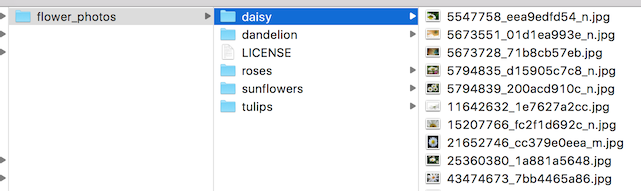
\includegraphics[scale=0.5]{folder_structure.png}
\end{figure}
\end{center}
实际上它会花一点时间得到你想要的精度,下面是一些常见的问题。
\subsection{创建一个训练图像集合}
首先我们需要查看收集到的图像,常见的问题是训练过程中数据的输入。

为了训练能起作用,每个你想要识别的图像你必须至少手机100张图片,你收集到的图片越多,训练的精确度可能越好。例如你拍摄一些蓝色的房间,另一些是绿色的房间模型的预测最终基于背景颜色,没有对象特征被考虑。为了避免这种情况,拍摄不同颜色的,没有一些实际能看到的的特征。如果你想了解更多这类问题你需要读\href{http://www.jefftk.com/p/detecting-tanks}{tank recognition}
如果你想考虑你用的分类。分隔大的数据集发现一些不同的物理形式为小的可以通过视觉区分的数据集,例如你可以用'vehicle'可以用来替代
'car','motobike'和'truck',考虑你有一个开放的世界还是封闭的世界将是很有价值的,在封闭的世界你唯一需要考虑的是识别已有的对象,例如一个植物识别的app你应该知道用户可能拍摄的花的图片,英雌你必须决定花的种类,相比之下一个巡逻机器人可能通过摄像头看到不同的事物。在这种情况下你想要分类器报告是否确认他看到的,这可能很难,但是你经常收集一些典型的和主体对象不相关的背景图像,,你可能会让它增加一些图片文件夹中未知的分类。
检查确保你的图像被正确的标记也是很重要的。经常用生成的标签对于你的目的来说是不可靠的,例如你用\#daisy命名一个叫Daisy的人。如果你想你的图像如果你了解你的图像,扫除任何错误将可能导致最后精确度提高。
\subsection{训练步骤}
如果你为你的图片感到高兴,你可以通过修改学习进程中的细节提升你的结果。最简单的方法是用--how\_many\_training\_steps。默认是4000.但是如果你增加到8000,他的训练时间将增加到两倍。精确度提高的比率显示你训练的越长一些点将停止,但是你可以试验什么时候达到你的模型的限制。
\subsection{扭曲}
随机通过变形,剪裁,变化输入图像的亮度是一个提高结果的常用方法,这样扩展了训练数据的大小,帮助网络学习
真是生活分类器所有的扭曲,在脚本中使用扭曲最大的缺点是缓冲瓶颈不再有用,因此输入图像将不能重用。这意味着训练京城可能花费更多时间,因此我推荐当着作为一个调节方法调节你的模型到合理。
你可以传递--random\_corp,--random\_scale和--random\_brightness给脚本扭曲图片。百分比值用来控制图片上扭曲用多少部分。,合理的值时5或者10.--flip\_left\_right将在水平方向随机的镜像图像的一半,有助有你的应用能理解翻转的图像。例如如果你想识别字母这将不是一个好的办法,因为翻转它们会毁掉原来的含义。
\subsection{超参数}
你可以调整一些参数查看是否对你的结果有帮助,--learning\_rate控制最终层训练更新的幅度。直观理解,如果这个值变小训练时间将边长,但是他可能对精度有帮助,你需要小心试验得到查看什么对于你的case生效了。--train\_batch\_size控制每一训练步多少图像被检查,因为学习率应用到每批上,如果你有更大的批得到相同的效果你将需要减小它。
\subsection{训练,验证,测试集}
当你为你的脚本指定图像文件夹时,文件夹被分成不同的数据集。最大的数据及是训练集,训练集包含用于训练网络的数据,用于更新权重。你也许很想知道为什么我们不用所有的图像训练?一个道德潜在的问题是当我们做机器学习算法时我们的模型会记住接近正确答案的不相关信息,你可以想想你的图像可能记住了一些照片的背景,通过标签匹配对象,它在训练时所有的图像可能产生一个好的结果,但是不能再新的图像产生好的结果因为他不能泛化对象的特征,仅仅在训练图像的时候记住了一些不重要的特征。
这个问题被称为过拟合,为了避免过拟合我们保持我们的一些数据不再训练进程中,因此模型不能记住他们,我们用这些图像作为检察确保过拟合没有发生,当我们在看模型在这些数据上有一个好的精度说明过拟合没有发生,通常80\%的数据被用来作为训练集10\%的数据集用来验证最后10\%的数据用做测试集预测分类器在真实世界的性能,通过--testing\_percentage和--validation\_percentage标志用来控制比例。通常你应该能留下一些值作为默认,不应该找到任何好处训练调整他们。
注意这个脚本用图象的文件名区分训练集,验证集,测试集中的图像(不是一个随机的函数),这样保证运行时图片不会再训练集和测试集之间移动,因为当用于训练模型的图像被验证集中的图像取代时可能会出现一些问题。
你也需注意到了在迭代过程中验证正确度的波动。多数波动是验证集的子集的随机性引起的,选择的验证集用来验证精确度。波动能能被最大层度减少,花费的训练时间增长,通过选择--validation\_batch\_size=-1用整个验证集计算精度。
当训练结束后你将能检查测试集中错误分类图像,这可以通过增加--print\_misclassified\_test\_images标记,这对于找到那些什么类型的图片让模型困惑(很难区别的)是很有帮助的例如你也许发现了一些种类一些常见的图像角度是特别难是别的,这样是鼓励你增加更多类型的分类训练子类,检查催哦五分类图片也指出输入数据中的错误,向错误标签,其质量魔术的照片。然而,你应该避免测试集固定点单个误差,因为他们仅仅反映在训练集中更多的问题。
\subsection{更对模型架构}
这个脚本默认用Inception v3模型架构作为预先训练脚本。这是一个好的开始的地方,因为它提供了高精度的训练结果,但是如果你想部署你的模型到手机设备或者其他的资源限制的环境你也许想要这种精确度换区更小的文件尺寸和更快的速度。
为了帮助这个\href{https://github.com/tensorflow/tensorflow/blob/master/tensorflow/examples/image_retraining/retrain.py}{retrain}
在\href{https://research.googleblog.com/2017/06/mobilenets-open-source-models-for.html}{移动架构}上支持30个不同的变量。
这里有一些比Inception v3更小精度的,但是可以得到更小的文件大小(下载小于兆字节)运行快乐几倍。为了训练这个模型,传递--architecture标志,例如:
\begin{lstlisting}{language={ANSI}C}
python tensorflow/examples/image_retraining/retrain.py \
    --image_dir ~/flower_photos -- architecture mobilenet_0.25_128_quantized
\end{lstlisting}
这将在/temp/创建一个941KB模型文件output\_graphi.pb.Mobilenet的25\%的参数,占据$128\times128$大小的输入图像,权重在磁盘中量化为8位,你可以选择'1.0','0.75','0.50','0.25'控制权重参数的数量,因此文件尺寸(和一些扩展速度),'224','192','160'或者'128'对于输入图像的尺寸,更小的尺寸更快的速度,选项'\_quantized'预示着是否文件应该包含8位或者32位浮点权重。速度和大小好处带来的是精确度的损失,但是对于一些用途来说是不重要的,他可以通过训练数据提高、例如用扭曲在花数据集允许你得到得到80\%的精度,甚至0.25/128、quantized图。
如果你在你的程序或者label\_image中用Mobilenet模型,你讲需要一个输入一个指定大小的图像转换一个浮点让位到'input' tensor,典型的24位乳香范围[0,255]你必须用(image-128.)/128转化它到[-1,1]范围。
\section{TF layer向导:建立一个卷积神经网络}
TensorFlow\href{https://www.tensorflow.org/api_docs/python/tf/layers}{layers module}是一个用于轻松建立神经网络的高级API,它提供了一个方法促进创建dense(全连接)层和卷积层,增加激活函数,应用dropout规则。在这个导航中,你讲学习如何用layers建立一个卷积神经网络模型识别手写体数据集。
\textbf{手写体数据集包含0-9,60000个训练样本10000个测试样本,图像格式为}$28\times28$
\subsection{开始}
创建文件cnn\_mnist.py,在手写体程序中添加如下代码:
\begin{python}
from __future__ import absolute_import
from __future__ import division
from __future__ import print_function

# Imports
import numpy as np
import tensorflow as tf

tf.logging.set_verbosity(tf.logging.INFO)

# Our application logic will be added here

if __name__ == "__main__":
  tf.app.run()
\end{python}
正如你看到的,你将增加,构造,训练,评估卷积神经网络,最终代码可以点击\href{https://www.github.com/tensorflow/tensorflow/blob/r1.3/tensorflow/examples/tutorials/layers/cnn_mnist.py}{这里}
\subsection{介绍卷积神经网络}
卷积神经网络是当前最先进的用于图像分类任务的模型架构。CNNs应用一些滤波器从原始的图像像素中提取高级特征,这个模型可能被用在分类。CNN包含三个组件:
\begin{itemize}
  \item \textbf{卷积层} 应用指定数量的卷积滤波器在图像上。对于每一个子区域,layer执行一系列数学操作生成一个单个值在输出feature map,卷积层然后应用relu激活函数输出非线性。
  \item \textbf{池化层} 下采样卷积层的图像数据,减小feature map的维度从而减小处理时间。常用池化算法是最大池化(提取feature map子区域)保留最大值,丢掉其它值。
  \item \textbf{Dense layers(全连接层)}在通过卷积层和下采样层特征提取执行分类。在全连接层,每一个节点连接到前面的节点。
\end{itemize}
通常CNN有一个卷积模块组成,每个层有卷积模块和池化模块组成。最新的卷积模块有一个或者更多的全连接层链接执行分类。最终CNN的全连接层包含每个目标类的一个单个节点(所有模型可能预测的类),用sofymax函数生成一个0-1的值(所有值的和维1)。我们可以解释给定图像和目标的相似情况。
\subsection{建立CNN MNIST分类器}
用CNN架构建立模型分类MNIST数据集。
\begin{enumerate}
  \item 卷积层1:应用$5\times5$卷积核(提取$5\times5$像素的区域),用relu激活函数。
  \item 池化层1:执行最大池化$2\times2$stride=2(指定的池化区域不重叠)
  \item 卷积层2:应用64个$5\times5$的卷积核,激活函数为relu。
  \item 池化层2:再次执行最大池化操作(卷积核$2\times2$)strider=2。
  \item Dense1:1024个神经元,dropout=0.4。
  \item Dense2:10个神经元0-9。
\end{enumerate}
打开cnn\_mnist.py增加下面的符合TensorFlow's Estimator api接口的cnn\_model\_fn函数。cnn\_mnist.py接受mnist特征数据,标签,\href{https://www.tensorflow.org/api_docs/python/tf/estimator/ModeKeys}{模型}作为参数,配置CNN,返回预测,损失,训练操作。
\begin{python}

\end{python}
下面的章节函数深入tf.layers代码创建每一层,如何计算loss,配置训练操作,生成预测。auguries你已经体验过CNN设TensorFlow Estimators,你可以跳到\href{https://www.tensorflow.org/tutorials/layers#training-and-evaluating-the-cnn-mnist-classifier}{Training and Evaluating the CNN MNIST Classifier}
\subsection{输入层}
 这个方法为二维图像数据创建见卷积和池化,输入tensor的形状为[batch\_size,image\_width,image\_height,channels]
\begin{itemize}
\item batch\_size:在训练过程执行提图下降的样本数据的子集大小。
\item image\_width:样本图像的宽。
\item image\_height:样本图像的高。
\item channels:样本图像的颜色通道,对于彩色图想,通道为3,对于单色图像通道为1.
\end{itemize}
在这里,我们的MNIST数据集由$28\times28$像素的单色照片组成,因此输入层的形状为[batch\_size,28,28,1],转变我们的feature map到这个形状,你可以执行操作:
\begin{python}
input_layer = tf.reshape(features["x"],[-1,28,28,1])
\end{python}
这里的-1表示输入的features["x"]的值的batch size应该被动态计算,保持所有的其它维度为常数。这允许我们将batch\_size作为一个可以调节的超参数。例如,如果我们输入样本到我们的batchs是5的模型,features["x"]将包含3920($5\times28\times28$)值(每一个值代表一个像素点),input\_layer形状将为[5,28,28,1],类似的如果我们样本的batchs是1000,features["x"]将包含78400个值,input\_layer形状将为[100,28,28,1]。
\subsection{第一层卷积层}
在我们的卷积层我想用32个$5\times5$的卷积核到输入层,用ReLU激活函数,我们一可用conv2d()方法创建这个层:
\begin{python}
conv1 = tf.layers.conv2d(
    inputs=input_layers,
    filters=32,
    kernel_size=[5,5],
    padding="same",
    activation=tf.nn.relu
)
\end{python}
\begin{displayquote}
inputs参数指定我们的输入tensor(形状为[batch\_size,image\_width,image\_height,channels]),这里,我们链接我们的第一个吉安基层到输入层,形状为[batch\_size,28,28,1]
注意:如果传递参数data\_format=channels\_first,conv2d()接受[channels,batch\_size,image\_width,image\_height]形状的数据。
\end{displayquote}
filter参数制定卷积核的个数,这里卷积核为32个。kenel\_size制定卷积核的维度为[width,height](这里[5,5])
padding参数制定两个值:valid(默认),和same。制定输出tensor应该有和输入特纳是哦然相同的形状,我们设置padding=same,说明TensorFLow增加0值到输出tensor的边缘波啊池宽度和高度为28(没有padding$5\times5$卷积$28\times28$将生成$24\times24tensor$,在$28\times28$用$5\times5$提取出$24\times24$个位置)。
activation参数指定应用到输出的激活函数,这里我们只顶tf.nn.relu。
conv2d()的输出形状为[batch\_size,28,28,32]:和输入有相同的宽度和高度,但是有32个通道保持每个卷积核的输出。
\subsection{池化层1}
链接我们创建的卷积层和池化层,我们在layers中用max\_pooling2d()方法构造执行最大池化,卷积核filter大小为$2\times2$,stride为2。
\begin{python}
pool1 = tf.layers.max_pooling2d(inputs=conv1, pool_size=[2, 2], strides=2)
\end{python}
再次,inputs制定输入tensor,形状为[batch\_size,image\_width,image\_height,channels],这里我们的输入tensor是第一层卷积层的输出conv1,形状为[batch\_size,28,28,32]

pool\_size指定最大池化filter的大小作为[width,height](这里是[2,2])如果两个维度相等你可以指定pool\_siz=2。
strides参数制定stride的大小,这里我们设置strdes为2,表示通过filter提取子区域的时候宽度和高度都是2像素。如果你想设置不同的width和height,你可以制定一个元祖或者列表。

我们的输出特纳是哦然和max\_pooling2d(pool1,形状为[batch\_size,14,14,32])相乘:$2\times2$减少宽度和高度到50\%。
\subsection{二层卷积和池化}
我们用conv2d()和max\_pooling2d()链接卷积和池化。对于卷积层2,我们配置64个$5\times5$的卷积核,激活函数为ReLU,池化层2,我们用和池化层一眼个间隔:
\begin{python}
conv2 = tf.layers.conv2d(
    inputs=pool1,
    filters=64,
    kernel_size=[5, 5],
    padding="same",
    activation=tf.nn.relu)

pool2 = tf.layers.max_pooling2d(inputs=conv2, pool_size=[2, 2], strides=2)
\end{python}
卷积层用pool1作为输入,生成tensor conv2。conv2形状为[atch\_size,14,14,64],和pool1的宽和高相等,64个通道因为64个卷积核。

池化层2那conv2作为输入,生成pool2作为输出,pool2形状[batch\_size,7,7,64](减少conv2 50\%的宽度和高度)
\subsection{Dense layer}
我们添加dense层(1024个神经元和ReLU激活函数)到CNN生成卷积/池化层提取的特征分类,我们将flatten我么呢feature map(pool2)到形状[batch\_size,features],因此我们的tensor有两维,上面的形状变成了[batch\_size,$7\times7\time64$]:
\begin{python}
pool2_flat = tf.reshape(pool2, [-1, 7 * 7 * 64])
\end{python}
现在哦我们用dense方法链接我们的dense:
\begin{python}
dense = tf.layers.dense(inputs=pool2_flat, units=1024, activation=tf.nn.relu)
\end{python}
inputs参数制定输入tensor:我们的flattened的feature map pool2\_flat。units参数指定dense层的神经元的数量。activation参数获取激活函数,这里我们依然是用tf.nn.relu。
为了改进我们的模型,我们也应用dropout方法正则化dense层。
\begin{python}
dropout = tf.layers.dropout(
    inputs=dense, rate=0.4, training=mode == tf.estimator.ModeKeys.TRAIN)
\end{python}
inputs参数和上面一样,rate参数制定dropout比率,这里用0.4表示40\%的元素将在训练中被随机丢弃。training参数得到一个bool行值制定是否模型在训练模式下运行,dropout仅仅在training为True时执行。这里我们检查是否mode传递给我们cnn\_model\_fn的模型函数是TRAIN模式。输出形状为[batch\_size,1024]
\subsection{Logits Layers}
在我们神经网络的最后一层是logits层,然会预测的原始值。我们用10个神经元创建一个dense layers,激活函数哦认为线性激活函数。
\begin{python}
logits = tf.layers.dense(inputs=dropout, units=10)
\end{python}
我们最终输出CNN的tensor,logits形状为[batch\_size,10]。
\subsection{常见的预测}
logits层返回我们预测的原始值(形状[batch\_size,10])。让我们转化这些原始值到我们的模型函数能返回的两种个不同的格式。
\begin{itemize}
\item predicted class:数字0-9。
\item probabilities:对于每个可能的目标类的概率。
\end{itemize}
对于更定的例子,我们的预测类是在相关行logts列有最大的值。我们可以用该tf.argmax函数找到这个元素的索引。
\begin{python}
tf.argmax(input=logits, axis=1)
\end{python}
input参数制定需要提取最大值的tensor,axis参数制定输入tensor沿着哪个轴寻找最大值。这里我们写着1轴寻找最大值。
我们可以用softmax生成概率。
\begin{python}
tf.nn.softmax(logits, name="softmax_tensor")
\end{python}
我们融合我们的预测到一个字典中,返回一个EstimatorSpec对象。
\begin{python}
predictions = {
    "classes": tf.argmax(input=logits, axis=1),
    "probabilities": tf.nn.softmax(logits, name="softmax_tensor")
}
if mode == tf.estimator.ModeKeys.PREDICT:
  return tf.estimator.EstimatorSpec(mode=mode, predictions=predictions)
\end{python}
\subsection{计算Loss}
对于训练和评估阶段,我们需要定义损失函数衡量我们的模型的预测如何接近目标类。对于想MNIST的多个分类问题,\href{https://en.wikipedia.org/wiki/Cross_entropy}{cross entropy}是典型的被用做损失度量。下面的代码计算交叉熵返回TRAIN或者EVAL模式:
\begin{python}
onehot_labels = tf.one_hot(indices=tf.cast(labels, tf.int32), depth=10)
loss = tf.losses.softmax_cross_entropy(
    onehot_labels=onehot_labels, logits=logits)
\end{python}
我们的labels tensor包含一个预测列表,像[1,9,\ldots],为了计算交叉熵,你需要转换labels为相关的\href{https://www.quora.com/What-is-one-hot-encoding-and-when-is-it-used-in-data-science}{one-hot encoding}
\begin{python}
[[0, 1, 0, 0, 0, 0, 0, 0, 0, 0],
 [0, 0, 0, 0, 0, 0, 0, 0, 0, 1],
 ...]
\end{python}
womenyoingtf.one\_hot函数执行转换。tf.one\_hot()有两个参数:
\begin{itemize}
\item one-hot tensor有值的位置,如上面1,表示位置索引为1的地方有1
\item depth:one-hot tensor的深度,目标类的数量,这里depth为10,
\end{itemize}
下面的代码为我们的labels创建一个one-hot tensor,onehot\_labels:
\begin{python}
onehot_labels = tf.one_hot(indices=tf.cast(labels, tf.int32), depth=10)
\end{python}
因为labels包含值从0-9,indices是我们的labels tensor,值变为证书。depth是10因为我们有10个可能的目标类。
下一步我们计算onehot\_labels的交叉熵和我们的logits层的softmax预测。tf.losses.softmax\_cross\_entropy()得到onehot\_labels和logits作为参数。在logits上执行softmax激活函数,返回损失的标量tensor:
\begin{python}
loss = tf.losses.softmax_cross_entropy(
    onehot_labels=onehot_labels, logits=logits)
\end{python}
\subsection{配置训练操作}
在先前的操作中我们为我们的CNN定义了损失作为logits层和layers的softmax cross-entropy。让我们配置我们的模型在训练落成中优化loss。我们将用0.001学习率和\href{https://en.wikipedia.org/wiki/Stochastic_gradient_descent}{SGD}作为优化算法\begin{python}
if mode == tf.estimator.ModeKeys.TRAIN:
  optimizer = tf.train.GradientDescentOptimizer(learning_rate=0.001)
  train_op = optimizer.minimize(
      loss=loss,
      global_step=tf.train.get_global_step())
  return tf.estimator.EstimatorSpec(mode=mode, loss=loss, train_op=train_op)

\end{python}
\subsection{增加评估度量}
为了增加度量到我们的模型,我们在EVAL定义了eval\_metric\_ops字典:
\begin{python}
eval_metric_ops = {
    "accuracy": tf.metrics.accuracy(
        labels=labels, predictions=predictions["classes"])}
return tf.estimator.EstimatorSpec(
    mode=mode, loss=loss, eval_metric_ops=eval_metric_ops)
\end{python}
\section{训练评估CNN MNIST分类器}
我们已经构建了MNIST CNN模型函数,现在我们准备训练评估它。
\subsection{载入训练和测试数据}
增加main()函数到cnn\_mnist.py载入训练数据和测试数据。
\begin{python}
def main(unused_argv):
  # Load training and eval data
  mnist = tf.contrib.learn.datasets.load_dataset("mnist")
  train_data = mnist.train.images # Returns np.array
  train_labels = np.asarray(mnist.train.labels, dtype=np.int32)
  eval_data = mnist.test.images # Returns np.array
  eval_labels = np.asarray(mnist.test.labels, dtype=np.int32)
\end{python}
我们存储训练数据train\_data(55000张原始图像的像素值)训练train\_labels(每张图片0-9)作为numpy数组.类似的我们存储评估数据(10000张)eval\_data和eval\_labels。
\subsection{创建Estimator}
下一步创建一个Estimator(一个用于执行高级模型训练,评估,推理的TensorFlow类),增加下面代码到main()中。
\begin{python}
# Create the Estimator
mnist_classifier = tf.estimator.Estimator(
    model_fn=cnn_model_fn, model_dir="/tmp/mnist_convnet_model")
\end{python}
model\_fn参数指定用于训练,评估,预测的模型函数,我们传递cnn\_model\_fn,models\_dir参数制定模型素据的保存目录为/tmp/mnist\_convnet\_model。
\subsection{建立Logging Hook}
因为CNN可能花一会训练,让我们设置一些采集以至于我们在训练时能跟踪进层。我们用TensorFlow的tf.train.SessionRunHook创建一个tf.train.LogginTensorHook采集从softmax层来的概率值,增加下面代码到main():
\begin{python}
# Set up logging for predictions
  tensors_to_log = {"probabilities": "softmax_tensor"}
  logging_hook = tf.train.LoggingTensorHook(
      tensors=tensors_to_log, every_n_iter=50)
\end{python}
我们存储一个我们想要采集进tensors\_to\_log的tensor词典。每个key是我们选择的label,将在采集输出被打印,相关的label是TensorFlow图的Tensor的名字,这里我们的概率可以在softmax\_tensor中找到,我们给我们softmax操作的名字在cnn\_model\_fn生成概率。

下一步我们创建LogginfTensorHook,传递tensor\_to\_log到tensors参数,我们设置every\_n\_iter=50,制定训练的时候每50步采集概率。
\subsection{选练模型}
现在我们准备好训练我们的模型,我们通过创建train\_input\_fn和在mnist\_classifier调用train(),增加下面到main()
\begin{python}
# Train the model
train_input_fn = tf.estimator.inputs.numpy_input_fn(
    x={"x": train_data},
    y=train_labels,
    batch_size=100,
    num_epochs=None,
    shuffle=True)
mnist_classifier.train(
    input_fn=train_input_fn,
    steps=20000,
    hooks=[logging_hook])
\end{python}
在Numpy\_input\_fn调用的时候,我们传递训练特征数据和标签给x和y。我们设置batch\_size是100(模型训练的时候每次最小批次是100个样本)。num\_epochs=None意味着模型将训练直到指定步数到达。我们也设置shuffle=True打暖训练数据,在训练调用的时候,我们设置steps=20000(这意味着模型总共训练20000次)我们传递looging\_hook去hooks参数,以至于它将在训练期间被触发。
\subsection{评估模型}
当训练结束是我们想要在测试及评估我们的模型,我们可以调用evaluate方法,在model\_fn指定eval\_metric\_ops参数度量方法:
\begin{python}
# Evaluate the model and print results
eval_input_fn = tf.estimator.inputs.numpy_input_fn(
    x={"x": eval_data},
    y=eval_labels,
    num_epochs=1,
    shuffle=False)
eval_results = mnist_classifier.evaluate(input_fn=eval_input_fn)
print(eval_results)
\end{python}
为了创建eval\_input\_fn,我们设置num\_epochs=1,因此模型评估在一个时期评估数据返回结果。我们也设置shuffle=False通过数据序列迭代。
\subsection{运行模型}
下面是采集的输出:
\begin{lstlisting}
INFO:tensorflow:loss = 2.36026, step = 1
INFO:tensorflow:probabilities = [[ 0.07722801  0.08618255  0.09256398, ...]]
...
INFO:tensorflow:loss = 2.13119, step = 101
INFO:tensorflow:global_step/sec: 5.44132
...
INFO:tensorflow:Loss for final step: 0.553216.

INFO:tensorflow:Restored model from /tmp/mnist_convnet_model
INFO:tensorflow:Eval steps [0,inf) for training step 20000.
INFO:tensorflow:Input iterator is exhausted.
INFO:tensorflow:Saving evaluation summary for step 20000: accuracy = 0.9733, loss = 0.0902271
{'loss': 0.090227105, 'global_step': 20000, 'accuracy': 0.97329998}
\end{lstlisting}
我们在测试集上获得了97.3\%的精确度。
\section{图像识别}
我们的大脑看东西很简单,他不需要得到任何人的告诉就能分别狮子,鲸钱包,读一个符号或者识别人脸,
但是计算机解决这个问题却很难。最近几年机器学习已经在这个问题上取得了很大的进步,事实上我们已经发现了一个称谓CNN的模型可以在很难的视觉认知邻域上获得匹敌甚至超过人类的性能。研究人员在ImageNet上展示他们的计算机视觉的成果,模型性能持续提升从\href{http://static.googleusercontent.com/media/research.google.com/en//archive/unsupervised_icml2012.pdf}{QuocNet},\href{http://www.cs.toronto.edu/~fritz/absps/imagenet.pdf}{AlexNet},\href{http://arxiv.org/abs/1409.4842}{Inception(GoogleNet)},\href{http://arxiv.org/abs/1502.03167}{BN-inception-v2},Google累不和外部的研究人员都已经出版了一些论文描述这些模型,但是结果任然河南再次提升,我们用下面的代码实现我们最新的模型\href{http://arxiv.org/abs/1512.00567}{Inception-v3},Inception-v3 2012年在Imagenet的LVRC上训练,这对计算机来说是一个基本的任务,这里模型尝试着分类整个图形为1000中分类像"斑马","大麦町犬","洗碗机",下面是AlexNet分类的一些图像:
\begin{center}
\begin{figure}[H]
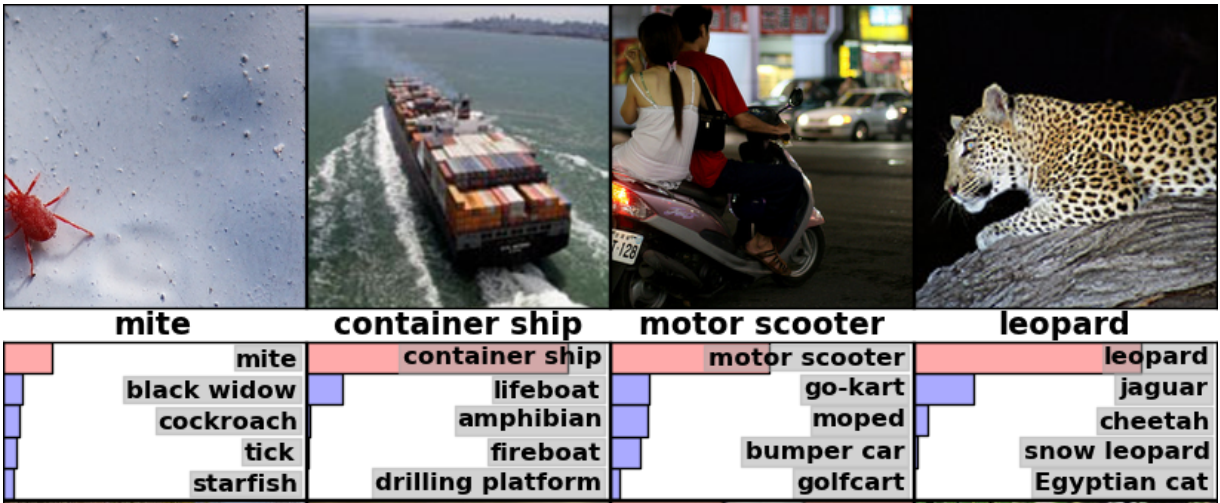
\includegraphics{AlexClassification.png}
\end{figure}
\end{center}
为了对比模型,我们检查迷行预测正确结果为"top-5 error rate",AlexNet2012年的验证数据及上得到top-5 error rate 15.3\%,Inception(GoogleLeNet)得到6.67\%,BN-Inception-v2得到4.9\%,Inception-v3得到3.46\%。
\begin{quote}
\emph{人类在ImageNet中做的怎么样,由 Andrej Karpathy 的\href{http://karpathy.github.io/2014/09/02/what-i-learned-from-competing-against-a-convnet-on-imagenet/}{博客}尝试测量人们的性能,他得到了5.1\%的top-5 error rate}
\end{quote}
下面的导航将教你如何使用Inception-v3.你将学习用Python或者C++学习分类图像成1000类,我们也将讨论如何从模型提取高级特征重用到其它的视觉任务。
\subsection{用Python API}
第一次运行时classify\_image.py将从tensorflow官网下载训练好的模型,你将需要200M左右的硬盘空间。开始从github上clone\href{https://github.com/tensorflow/models}{Google模型},然后运行命令:
\begin{lstlisting}[language=Bash]
cd models/tutorials/image/imagenet
python classify_image.py
\end{lstlisting}
上面的命令将分类下面的熊猫图片。
\begin{center}
\begin{figure}[h]
\includegraphics{cropped_panda.jpg}
\end{figure}
\end{center}
如果模型正确运行将生成下面的输出:
\begin{lstlisting}{language=Python}
giant panda, panda, panda bear, coon bear, Ailuropoda melanoleuca (score = 0.88493)
indri, indris, Indri indri, Indri brevicaudatus (score = 0.00878)
lesser panda, red panda, panda, bear cat, cat bear, Ailurus fulgens (score = 0.00317)
custard apple (score = 0.00149)
earthstar (score = 0.00127)
\end{lstlisting}
如果你希望添加其它的JPEG图片,你也许需要编辑--image\_file参数,如果你需要下载模型数据到不同的目录,你将需要指定--model\_dir到使用的目录。
\subsection{用C++ API}
你可以在生产环境上使用C++运行相同的Inception-v3模型。你可以下载包含像这样定义的GraphDef的打包文件
(从TensorFlow仓库的根目录运行)
\begin{lstlisting}[language=Bash]
curl -L "https://storage.googleapis.com/download.tensorflow.org/models/inception_v3_2016_08_28_frozen.pb.tar.gz" |
  tar -C tensorflow/examples/label_image/data -xz
\end{lstlisting}
下一步我们编译包含C++代码载入的二进制运行图,如果你已经按照\href{https://www.tensorflow.org/install/install_sources}{the instructions to download the source installation of TensorFlow}
配置了你的平台,你将能在shell终端通过下面的命令构建例子运行:
\begin{lstlisting}[language=Bash]
bazel build tensorflow/examples/label_image/...
\end{lstlisting}
你可以像这样创建一个二进制的执行文件:
\begin{lstlisting}[language=Bash]
bazel-bin/tensorflow/examples/label_image/label_image
\end{lstlisting}
用框架默认的例子图片,输出下面的结果:
\begin{lstlisting}[language=Bash]
I tensorflow/examples/label_image/main.cc:206] military uniform (653): 0.834306
I tensorflow/examples/label_image/main.cc:206] mortarboard (668): 0.0218692
I tensorflow/examples/label_image/main.cc:206] academic gown (401): 0.0103579
I tensorflow/examples/label_image/main.cc:206] pickelhaube (716): 0.00800814
I tensorflow/examples/label_image/main.cc:206] bulletproof vest (466): 0.00535088
\end{lstlisting}
在这个例子中你用一张默认的图片\href{https://en.wikipedia.org/wiki/Grace_Hopper}{Admiral Grace Hopper},你可以看到网络正确识别她的军官制服,得分0.8。
\begin{center}
\begin{figure}[H]
\includegraphics{grace_hopper.jpg}
\end{figure}
\end{center}
下一步提供--image=参数分辨你的图片
\begin{lstlisting}[language=Bash]
bazel-bin/tensorflow/examples/label_image/label_image --image=my_image.png
\end{lstlisting}
如果你查看\href{https://github.com/tensorflow/tensorflow/blob/master/tensorflow/examples/label_image/main.cc}{tensorflow/examples/label\_image/main.cc}你可以明白它是如何工作的,我们希望代码能帮你整合TensorFlow到你的应用,因此我们将一步步的浏览主函数。命令行参数控制文件从哪里载入,即输入图像的内容。模型希望得到$299\times299$的RGB图像,分别是input\_width,input\_height,我们需要缩放图像的像素从0-255到图能操作的一个浮点值。我们通过input\_mean和input\_std控制缩放:我们首先用像素值减去input\_mean然后除以input\_std,这些值看起来可能有点琢磨不透,但是他们被原始作者定义,她/他想训练的时候什么值被匹配,你可以看看我们如何在\href{https://github.com/tensorflow/tensorflow/blob/master/tensorflow/examples/label_image/main.cc#L88}{ReadTensorFromImageFile()}函数中如何应用一张图像。
\begin{lstlisting}[language=C++]
// Given an image file name, read in the data, try to decode it as an image,
// resize it to the requested size, and then scale the values as desired.
Status ReadTensorFromImageFile(string file_name, const int input_height,
                               const int input_width, const float input_mean,
                               const float input_std,
                               std::vector<Tensor>* out_tensors) {
  tensorflow::GraphDefBuilder b;
\end{lstlisting}
我们开始撞见亿个GraphDefBuilder对象指定一个运行或者载入的模型。
\begin{lstlisting}[language=C++]
  string input_name = "file_reader";
  string output_name = "normalized";
  tensorflow::Node* file_reader =
      tensorflow::ops::ReadFile(tensorflow::ops::Const(file_name, b.opts()),
                                b.opts().WithName(input_name));
\end{lstlisting}
然后我们开始为我们想要运行或者载入的小模型创建节点,变换大小,缩放像素值得到主函数希望得到的结果,我们创建的第一个节点是保持图像名字的tensor想要载入Const操作然后作为第一个输入传入ReadFile操作,你也许注意到我们传递b.opts()操作给所有的创建操作,参数确保节点被添加到GraphDefBuilder的模型定义。这给了一个名字给节点,
对于给一个名字节点不是严格需要的因为如果你不指定这个将自动命名,但是它使得调试变得简单
\begin{lstlisting}[language=C++]
  // Now try to figure out what kind of file it is and decode it.
  const int wanted_channels = 3;
  tensorflow::Node* image_reader;
  if (tensorflow::StringPiece(file_name).ends_with(".png")) {
    image_reader = tensorflow::ops::DecodePng(
        file_reader,
        b.opts().WithAttr("channels", wanted_channels).WithName("png_reader"));
  } else {
    // Assume if it's not a PNG then it must be a JPEG.
    image_reader = tensorflow::ops::DecodeJpeg(
        file_reader,
        b.opts().WithAttr("channels", wanted_channels).WithName("jpeg_reader"));
  }
  // Now cast the image data to float so we can do normal math on it.
  tensorflow::Node* float_caster = tensorflow::ops::Cast(
      image_reader, tensorflow::DT_FLOAT, b.opts().WithName("float_caster"));
  // The convention for image ops in TensorFlow is that all images are expected
  // to be in batches, so that they're four-dimensional arrays with indices of
  // [batch, height, width, channel]. Because we only have a single image, we
  // have to add a batch dimension of 1 to the start with ExpandDims().
  tensorflow::Node* dims_expander = tensorflow::ops::ExpandDims(
      float_caster, tensorflow::ops::Const(0, b.opts()), b.opts());
  // Bilinearly resize the image to fit the required dimensions.
  tensorflow::Node* resized = tensorflow::ops::ResizeBilinear(
      dims_expander, tensorflow::ops::Const({input_height, input_width},
                                            b.opts().WithName("size")),
      b.opts());
  // Subtract the mean and divide by the scale.
  tensorflow::ops::Div(
      tensorflow::ops::Sub(
          resized, tensorflow::ops::Const({input_mean}, b.opts()), b.opts()),
      tensorflow::ops::Const({input_std}, b.opts()),
      b.opts().WithName(output_name));
\end{lstlisting}
我们然后添加更多的节点解码文件数据为图片,转化整数为浮点值,变形然后最后运行减去和除法操作:
\begin{lstlisting}[language=C++]
  // This runs the GraphDef network definition that we've just constructed, and
  // returns the results in the output tensor.
  tensorflow::GraphDef graph;
  TF_RETURN_IF_ERROR(b.ToGraphDef(&graph));
\end{lstlisting}
在这最后我们有一个存储在变量b中的模型定义我们用ToGraphDef()转化完整的图定义
\begin{lstlisting}[language=C++]
  std::unique_ptr<tensorflow::Session> session(
      tensorflow::NewSession(tensorflow::SessionOptions()));
  TF_RETURN_IF_ERROR(session->Create(graph));
  TF_RETURN_IF_ERROR(session->Run({}, {output_name}, {}, out_tensors));
  return Status::OK();
\end{lstlisting}
我们创建一个运行图的接口tf.Session对象,运行它,指定我们想从那个节点获得输出和放输出数据到哪里,这给我们一个Tensor对象的向量,这个对象将变成一个三个对量,你可以将Tensor认为是多维数组,它保存299像素宽,299像素高。3通道的图像作为浮点值,如果你有自己的图像处理框架,你应该能用它替代,只要你在输入图像到主图中时应用相同的转换。这是用C++创建一个简单的TensorFlow图的例子,但是对于预先训练好的Inception模型我们想从文件载入一个大的定义,你可以在LoadGraph()函数中查看我们如何做的:
\begin{lstlisting}[language=C++]
// Reads a model graph definition from disk, and creates a session object you
// can use to run it.
Status LoadGraph(string graph_file_name,
                 std::unique_ptr<tensorflow::Session>* session) {
  tensorflow::GraphDef graph_def;
  Status load_graph_status =
      ReadBinaryProto(tensorflow::Env::Default(), graph_file_name, &graph_def);
  if (!load_graph_status.ok()) {
    return tensorflow::errors::NotFound("Failed to load compute graph at '",
                                        graph_file_name, "'");
  }
\end{lstlisting}
如果你已经查看的图像载入代码,一些名词应该很熟悉。想必须用一个GraphDefBuffer残生一个GraphDef对象,我们载入一个包含GraphDef的protobuf文件。
\begin{lstlisting}[language=C++]
  session->reset(tensorflow::NewSession(tensorflow::SessionOptions()));
  Status session_create_status = (*session)->Create(graph_def);
  if (!session_create_status.ok()) {
    return session_create_status;
  }
  return Status::OK();
}
\end{lstlisting}
我们从GraphDef创建一个Session对象传递它给调用器以至于我们稍后能使用。GetTopLabels()函数有些像函数载入,但是我们希望运行主图得到结果,存储它进一个按照标签最高评分的结果,像图片载入,它创建一个的GraphDefBuilder,添加一对节点上去然后运行短图割刀一对输出tensor,在这个例子中他们代表排序的分数和最好可能性的结果的索引位置。
\begin{lstlisting}[language=C++]
// Analyzes the output of the Inception graph to retrieve the highest scores and
// their positions in the tensor, which correspond to categories.
Status GetTopLabels(const std::vector<Tensor>& outputs, int how_many_labels,
                    Tensor* indices, Tensor* scores) {
  tensorflow::GraphDefBuilder b;
  string output_name = "top_k";
  tensorflow::ops::TopK(tensorflow::ops::Const(outputs[0], b.opts()),
                        how_many_labels, b.opts().WithName(output_name));
  // This runs the GraphDef network definition that we've just constructed, and
  // returns the results in the output tensors.
  tensorflow::GraphDef graph;
  TF_RETURN_IF_ERROR(b.ToGraphDef(&graph));
  std::unique_ptr<tensorflow::Session> session(
      tensorflow::NewSession(tensorflow::SessionOptions()));
  TF_RETURN_IF_ERROR(session->Create(graph));
  // The TopK node returns two outputs, the scores and their original indices,
  // so we have to append :0 and :1 to specify them both.
  std::vector<Tensor> out_tensors;
  TF_RETURN_IF_ERROR(session->Run({}, {output_name + ":0", output_name + ":1"},
                                  {}, &out_tensors));
  *scores = out_tensors[0];
  *indices = out_tensors[1];
  return Status::OK();
\end{lstlisting}
PrintTopLabels()函数得到排序接轨哦用一种友好的方式打印他们。CkeckTopLabel()函数是非常累是,但是仅仅确保顶部的标签是我们想要的,用于调试。
在最后main()结合所有的函数调用
\begin{lstlisting}[language=C++]
int main(int argc, char* argv[]) {
  // We need to call this to set up global state for TensorFlow.
  tensorflow::port::InitMain(argv[0], &argc, &argv);
  Status s = tensorflow::ParseCommandLineFlags(&argc, argv);
  if (!s.ok()) {
    LOG(ERROR) << "Error parsing command line flags: " << s.ToString();
    return -1;
  }

  // First we load and initialize the model.
  std::unique_ptr<tensorflow::Session> session;
  string graph_path = tensorflow::io::JoinPath(FLAGS_root_dir, FLAGS_graph);
  Status load_graph_status = LoadGraph(graph_path, &session);
  if (!load_graph_status.ok()) {
    LOG(ERROR) << load_graph_status;
    return -1;
  }
\end{lstlisting}
我们载入主图:
\begin{lstlisting}[language=C++]
 // Get the image from disk as a float array of numbers, resized and normalized
  // to the specifications the main graph expects.
  std::vector<Tensor> resized_tensors;
  string image_path = tensorflow::io::JoinPath(FLAGS_root_dir, FLAGS_image);
  Status read_tensor_status = ReadTensorFromImageFile(
      image_path, FLAGS_input_height, FLAGS_input_width, FLAGS_input_mean,
      FLAGS_input_std, &resized_tensors);
  if (!read_tensor_status.ok()) {
    LOG(ERROR) << read_tensor_status;
    return -1;
  }
  const Tensor& resized_tensor = resized_tensors[0];
\end{lstlisting}
载入,变形,处理输入图像
\begin{lstlisting}[language=C++]
  // Actually run the image through the model.
  std::vector<Tensor> outputs;
  Status run_status = session->Run({ {FLAGS_input_layer, resized_tensor}},
                                   {FLAGS_output_layer}, {}, &outputs);
  if (!run_status.ok()) {
    LOG(ERROR) << "Running model failed: " << run_status;
    return -1;
  }
\end{lstlisting}
我们用图像作为输入运行载入的图:
\begin{lstlisting}[language=C++]
  // This is for automated testing to make sure we get the expected result with
  // the default settings. We know that label 866 (military uniform) should be
  // the top label for the Admiral Hopper image.
  if (FLAGS_self_test) {
    bool expected_matches;
    Status check_status = CheckTopLabel(outputs, 866, &expected_matches);
    if (!check_status.ok()) {
      LOG(ERROR) << "Running check failed: " << check_status;
      return -1;
    }
    if (!expected_matches) {
      LOG(ERROR) << "Self-test failed!";
      return -1;
    }
  }
\end{lstlisting}
出于测试的目的我们可以检查确保我们得到我们想要的结果:
\begin{lstlisting}[language=C++]
// Do something interesting with the results we've generated.
  Status print_status = PrintTopLabels(outputs, FLAGS_labels);
\end{lstlisting}
最后我们打印我们输出的标签:
\begin{lstlisting}[language=C++]
 if (!print_status.ok()) {
    LOG(ERROR) << "Running print failed: " << print_status;
    return -1;
  }
\end{lstlisting}
我们用TensorFLow的State对象处理错误,它很方便因为它用ok()作为检查器检查是否出现的任何错误,然后打印出可读的错误消息,在这个例子中我们一站式对象识别,但是你应该能用类似的代码在你发现的其他模型上或者自己训练在不同的领域。我们希望这个小的例子给你一些灵感如何用TensorFlow和你的产品。
\begin{quote}
转换学习是想法,如果你知道如何很好的解决问题,你应该能转换一些解决相关问题的理解,一种执行转换学习的方法是移除网络最后的分类层提取\href{http://arxiv.org/abs/1310.1531}{next-to-last layer of the CNN},在这个例子中2048维向量,有一个关于这个如何做到的向导\href{https://www.tensorflow.org/tutorials/image_retraining}{in the how-to section}
\end{quote}
\subsection{更多学习资源}
为了学习神经网络,Michael Nielsen的\href{http://neuralnetworksanddeeplearning.com/chap1.html}{free online book},类似对于卷积神经网络Chris Olah有一些\href{http://colah.github.io/posts/2014-07-Conv-Nets-Modular/}{nice blog posts},Michael Nielsen的书有一个关于它的\href{http://neuralnetworksanddeeplearning.com/chap6.html}{greatchapter covering them}为了找出更多的卷积神经网络的实现你可以调到\href{https://www.tensorflow.org/tutorials/deep_cnn}{ deep convolutional networks tutorial},最后如果你想加速在这一领域的研究,你可以读导航中列出的最近的相关工作的论文。
\section{TensorFlow实现大规模线性模型}
tf.estimator API 提供了一些丰富的工具在TensorFlow中处理线性模型,这个章节提供了一个官员这些工具的概览,解释如下:
\begin{itemize}
  \item 线性模型是什么
  \item 为什么你想用线性模型
  \item tf.estimator如何使得在TensorFlow中建立一个线性模型变得简单
  \item 如何结合线性模型和深度学习的有点
\end{itemize}
读这个概览决定了是否tf.estimator对于你来说有用,然后做一下\href{Models tutorial}{https://www.tensorflow.org/tutorials/wide}这个概览的代码来自于这个章节,但是导航更详细的调通代码。为了明白为了理解这个概念熟悉一些基本的机器学习概念和tf.estimator是有帮助的。
\subsection{什么是线性模型}
一个线性模型用一个特征权重和作出预测,例如,如果你有关于年龄。教育年数,每周工作小时数的数据,你可以的你可以你可以了解这些权重以至于他们的权重求和评估一个人的薪水。你可以用线性模型分类,一些线性模型转化权重为一个更方便的形式,例如逻辑回归转化权重和维逻辑函数输出0-1之间的数值。但是你依然有对于每个输入特征你依然有一个权重。
\subsection{为什么你想用线性模型?}
当最近的研究已经展示了有很多层的复杂神经网络的能力为什么我们想用一个简单的模型?\newline
线性模型:
\begin{itemize}
  \item 比深度神经网络训练快速
  \item 在大型数据及上也能工作的很好
  \item 训练的时候不要求微小的学习率
  \item 相比神经网络能更简单轻松地调试,你可以检查付给给个特征的权重找出那个对于预测结果的影响最大。
  \item 对于了解机器学习提供了很好的起点
  \item 工业上广泛的使用
\end{itemize}
\subsection{tf.estimator将如何构建线性模型}
你可以通过TensorFlow建立线性模型不需要特殊的API,但是tf.estimator提供了一些工具帮助你更轻松地构建搞笑的大规模线性模型。
\subsubsection{特征列和线性模型}
设计的线性模型的大部分工作是转化原始数据为合适的输入特征,TensorFlow用FeatureColumn概念启动这些转换,一个FeatureColumn代表你的数据的单个特征,一个FeatureColumn也许代表一些像"height"或者也许代表一个像"eye\_color"的种类这里的值是来自离散的可能性像{'blue', 'brown', 'green'}。连续的特征像'height'和绝对的特征'eye\_color',在输入模型前一个单个的值可能被转化为数值序列。FeatureColumn概念让你用但一个语义单元操作特征,你可以转化选择特征来包含没有用指定索引处理的处理。
\subsubsection{稀疏列}
绝对的特征在线性模型中被转化为稀疏向量,在向量中每个可能值有一个相关的索引或者id,例如如果仅仅有三个可能的颜色代表'eye\_color'作为长度为3的向量,'brown'将变为[1,0,0],'blue'将变成[0,1,0],'green'将变成[0,0,1],这里向量被称为稀疏因为当可能值很大的时候。它们可能很长但是有很多0。尽管我们不需要用绝对列用tf.estimator线性模型,一个有力的线性模型能处理大型的稀疏向量,tf,estimator线性模型工具的稀疏特征也正是一个主要的用途。
\subsubsection{编码稀疏列}
FeatureColumn用下面的代码自动处理传统的绝对的值称为向量:
\begin{lstlisting}[language=Python]
eye_color = tf.feature_column.categorical_column_with_vocabulary_list(
    "eye_color", vocabulary_list=["blue", "brown", "green"])
\end{lstlisting}
这里的eye\_color是你的源数据的列的名字,入股你不知道所有的可能值你可以为你的绝对特征以生成FeatureColumn。对于这种情况,你将用categorical\_column\_with\_hash\_bucket(),用一盒散列函数赋值索引给特征值。
\begin{lstlisting}[language=Python]
education = tf.feature_column.categorical_column_with_hash_bucket(
    "education", hash_bucket_size=1000)
\end{lstlisting}
\subsection{特征交叉}
因为线性模型赋值独立的权重给分开的特征,他们不嫩改写东西相对重要的指定特征值的结合。如果你有一个特征'favorite\_sport'和特征'home\_city'然后你想尝试预测一个是是否喜欢船红色的衣服,你的线性模型将不能从喜欢穿红色衣服的圣路易斯的棒球粉丝中学习。你可以通过创建一个新的特征'favorite\_sport\_x\_home\_city'得到这个限制。这些特征的值对一个人仅仅链接两个源特征'baseball\_x\_stlouis',例如这个结合的特征被称为特征交叉,crossed\_column()方法使得建立特征交叉很容易
\begin{lstlisting}[language=Python]
sport_x_city = tf.feature_column.crossed_column(
    ["sport", "city"], hash_bucket_size=int(1e4))
\end{lstlisting}
连续的列,你可以像这样指定一个连续的特征:
\begin{lstlisting}[language=Python]
age = tf.feature_column.numeric_column("age")
\end{lstlisting}
尽管作为一个简单的实数,连续特征经常能直接输入给模型,TensorFlow对于排序这列提供了有用的转化。
\subsection{Bucketization}
Bucketization转化一个连续的列为绝对列。这个转换让你在交叉特征中用连续的特征,或者了解那里指定值的范围特别重要,Bucketization分隔可能值的范围为字范围称为buckets。
\begin{lstlisting}[language=Python]
age_buckets = tf.feature_column.bucketized_column(
    age, boundaries=[18, 25, 30, 35, 40, 45, 50, 55, 60, 65])
\end{lstlisting}
bucket掉入那个区域变成这个值的绝对标签。

\subsubsection{输入函数}
FeatureColumn为你的模型提供了一个指定的输入数据。标志着着如何代表和转化数据。但是他们本身不提供数据,你通过输入函数提供数据,输入函数必须返回一个tensor字典,每个键是FeatureColumn的名字。每个键的值是一个对于所有数据实例是包含特征值的tensor。查看\href{https://www.tensorflow.org/get_started/input_fn}{ Building Input Functions with tf.estimator}获取更多的关于输入函数的见解,在\href{https://www.github.com/tensorflow/tensorflow/blob/r1.3/tensorflow/examples/learn/wide_n_deep_tutorial.py}{ linear models tutorial code}中的input\_fn是实现输入函数的一个例子。在输入函数被传递给train()和evaluate()调用初始训练和测试正如下一章描述的。
\subsubsection{线性estimator}
TensorFlow的estimator给训练和分类模型提供了一个独一无二的训练评估工具。他们考虑详细的训练和评估训练允许用户集中注意力在模型输入和架构上。

为了建立一个线性estimator,你可以用tf.estimator.LinearClassfier estimator或者tf.estimator.LinearRegressor estimator分别建立分类和回归模型。

创建tensorflow estimator和运行estimator:
\begin{itemize}
  \item estimator实例,对于两个线性estimator类,你传递一个FeatureColumn列表给构造器。
  \item 调用estimator的train()方法训练它
  \item 调用estimator的evaluate()方法看看它如何工作
\end{itemize}
例如:
\begin{lstlisting}[language=Python]
e = tf.estimator.LinearClassifier(
    feature_columns=[
        native_country, education, occupation, workclass, marital_status,
        race, age_buckets, education_x_occupation,
        age_buckets_x_race_x_occupation],
    model_dir=YOUR_MODEL_DIRECTORY)
e.train(input_fn=input_fn_train, steps=200)
# Evaluate for one step (one pass through the test data).
results = e.evaluate(input_fn=input_fn_test)

# Print the stats for the evaluation.
for key in sorted(results):
    print("%s: %s" % (key, results[key]))
\end{lstlisting}
\subsection{广泛深入的学习}
tf.estimator API提供一个estimator类让你结合训练一个模型和深度神经网络。这个出色的方法结合线性模型的能力存储神经网络泛化的能力关键特征。用tf.estimator.DNNLinearCombineClassfier创建一个广而深的模型:
\begin{lstlisting}[language=Python]
e = tf.estimator.DNNLinearCombinedClassifier(
    model_dir=YOUR_MODEL_DIR,
    linear_feature_columns=wide_columns,
    dnn_feature_columns=deep_columns,
    dnn_hidden_units=[100, 50])
\end{lstlisting}
更多信息请查看\href{https://www.tensorflow.org/tutorials/wide_and_deep}{Wide and Deep Learning tutorial}。
\chapter{扩展}
这个章节解释开发者如何增加功能到TensorFlow。
\section{TensorFlow架构}
我们设计TensorFlow是为了大规模分布式训练和推理,但是它也能灵活的支持一些新的机器学习模型实验和系统级别的优化。

这个文件描述了这个系统架构使得结合这个规模和灵活度成为可能。假设你熟悉TensorFlow基本的一些概念,像计算图,操作绘画。
这个文档适合于那些想用当前API不支持的一些方法扩展TensorFlow,想要优化TensorFlow的硬件工程师,在法规莫分布式系统上实现机器学习系统或者是任何想要了解TensorFlow的hood的人。读完它后你应该能读和修改TensorFlow核心代码。
\section{概述}
TensorFlow运行时是一个跨平台的库,下图画出了常用的架构,C API分隔用户代码和核心代码。
\begin{center}
\begin{figure}[H]
\includegraphics{layers.png}
\end{figure}
\end{center}
\begin{itemize}
\item \textbf{Client}
\item 定义计算作为数据流图。
\item 用session初始化图。
\item Distributed Master
\item 从图中修剪一个子图作为定义的参数给Session.run()
\item 分开不同的子图为多个部分在不同的进程和设备上运行。
\item 分配图块到worker service。
\item \textbf{Worker services}
\item 调度图上的操作在可用的硬件平台(CPUs,GPUs)上执行。
\item 发送和接收worker service的操作结果。
\item 内核实现。
\item 执行单个图操作的计算。
\end{itemize}
下图说明逐渐的交互。"job:worker/task:0"和"/job:ps/task:0"两个任务在wokers上。"PS"代表"parameter server":一个负责存储更新模型参数的任务。另一个任务优化参数时发送更新到这些参数,类似的在任务之间的分隔是不被要求的,但是它通常用于分配的训练。
%没有图像
\begin{figure}[H]
\includegraphics{diag1.png}
\end{figure}
注意Distributed Master和Worker Service仅仅存在于分布的TensorFlow。,单进程版本的TensorFlow包含一个特别的Session实现能做任何Distributed msdter能做的不仅仅是和本地进程通信。

下面的章节表述了TensorFlowlayer的核心。
\subsection{Client}
用户写TensorFlow程序构造计算图。这个车给需既可以直接组成单个操作或者用一个像Estimators API的方便的库组成神经网络乘和其他高级抽象。TensorFlow支持多种用户语言,但是我们优先使用Python和C++,仅仅是因为我们的内部用户熟悉他们。当特征被建立好后我们将他们接入C++。因此用户可以得到一个对所有语言优化的实现。大多数的训练库仅仅支持Python,但是C++支持更高效的推理。
用户创建一个绘画,发送图的定义到ditributed master作为tf.GraphDef 协议缓冲区。然后客户评估图上的一个节点或者多个节点,评估触发一个distributed master的调用初始化计算。

在下图中,客户建立一个图,应用权重(w)到特征向量(x),增加偏置(b)保存结果。
%没有图像
\begin{figure}[h]
\includegraphics[scale=0.5]{graph_client.png}
\end{figure}
\subsection{Distributed master}
\begin{itemize}
\item 修剪图得到子图计算用户的节点请求。
\item 对于每一个加入的设备,分隔图获得子图。
\item 缓存这些块以至于他们能用在自序列中。
\end{itemize}
因为master查看每一步的计算,它用像常用的子表达式消除和常数折叠的标准的优化。它然后执行优化的子图。
下图显示一个可能的分隔。distributed master有组合的模型参数为了放置他们在参数服务器上。
这里图的边缘被分隔,distributed master发送接收节点在不同的任务间传送信息。
下面的distributed master传输子图到分布的任务。
\subsection{Worker Service}
任务中的worker service。
\begin{itemize}
\item 处理master的请求。
\item 调度内核执行包含本地子图的操作
\item 任务间的直接通信。
\end{itemize}
我们偶化worker service为了能用更小的花销以女性大的图。我们当前的实现能实现每秒执行上万张子图,使得大量的副本快速的训练。worker service布置内核到本地设备上然后通过利用多CPU多GPU尽可能的并行执行。
我们为源和目的设备指定发送和接收操作。
\begin{itemize}
\item 用cudaMemcpyAsync() API在本地CPU和GPU之间转换,覆盖计算和数据的转化。
\item 用对等的DMA在不同的本地GPU之间转化避免通过主CPU的高昂代价。
\end{itemize}
对于任务间的转化,TensorFLow用多个协议,报错:
\begin{itemize}
\item gPRC over TCP
\item RDMA over COnverged Ethernet
\end{itemize}
我们对于NVIDIA的多GPU通信NCCL库有初步的支持,查看\href{}{tf.contrib.nccl}
\section{内核实现}
运行包含超过200个标准操作白扩数学,数组操作,控制流,状态管理操作。每一个操作对不同的设备有优化,一些操作内核用Eigen::Tensor实现,用C++模板生成在多核CPU和GPUs上生成高效的并行代码,然而我们优先像像CuDNN这类更高效实现的库。我们也实现了量化,能在移动设备和高流通数据中心应用上更快地推理,用gemmlowp地精读矩阵库加速量化计算。

如果很难或者抵消的表达子计算作为操作的组成,用户可以注册额外的京城通过C++提供更高效的实现,,我们推荐你duit一些重要的操作像ReLU和Sigmoid和相关的梯度注册你的融合内核,XLA变压器有意额实验性是实现自动内核融合。


\section{性能向导}
这个向导包含了一些很好的实践来优化你的TensorFlow代码。向导被分成下面的章节:
\begin{itemize}
\item 一般的最佳实践包括常用的多种模型和硬件
\item 优化GPU详细的技巧和GPU有关
\item CPU优化 详细的CPU特定信息
\end{itemize}
\subsection{一般的最佳实践}
最佳的实践包括下面章节:
\begin{itemize}
	\item 输入pipline优化
	\item 数据格式
	\item 常用的融合操作
	\item 从源代码构建和安装
\end{itemize}
\subsubsection{输入pipeline优化}
常用的模型从磁盘获取数据在通过网络发送数据之前提前处理它,例如模型按照下面处理JPEG图像:从磁盘载入图像,解码JPEG为tensor,剪切填充,可能还有翻转和扭曲,然后分批处理。下面的图是输入pipeline。正如GPU和其它的硬件极速器会更快,预处理数据可能成为一个瓶颈。如果输入pipeline是瓶颈可能变得很复杂。一个直接的方法是在输入pipeline后减少模型为单个操作,每秒测量样本。如果对于完整的模型和单个的模型没表中样本的差别很小不同的,输入pipeline可能是瓶颈。下面有一些其它的方法识别这个问题。
\begin{itemize}
	\item 通过\lstinline[language=Bash]{watch -n 2 nvidia-smi}检查GPU是否被完全使用。如果GPU利用没有达到80-100\%,输入pipeline可能是瓶颈。
	\item 生成时间线查看大模块空白。一个生成时间线的例子在\href{https://www.tensorflow.org/performance/xla/jit}{XLA JIT}
	\item 检查CPU使用。他可能有一个优化的pipeline和缺乏CPU循环处理pipeline
	\item 评估生产力需要和验证在这个生产力条件下磁盘使用。一些云方案有网络添加磁盘速度50MB/sec,这比机械硬盘的150/MS/sec和SATA SSD的500MB/sec,PCIe SSD的2000+
 MB/sec低得多\end{itemize}
 \subsubsection{在CPU上处理}
 防止输入pipeline在CPU上能极大地提高性能。利用CPU处理输入pipeline,GPU训练。确保预处理在CPU上,按照如下操作打包:
 \begin{lstlisting}[language=Python]
 with tf.device('/cpu:0'):
     # function to get and process images or data.
     distorted_inputs = load_and_distort_images()
 \end{lstlisting}
 如果你用tf.estimator.Estimator输入函数自动放置到CPU上。
 \subsubsection{用Dataset API}
 \href{https://www.tensorflow.org/programmers_guide/datasets}{Dataset API}防止queue\_runner作为推荐的API建立输入pipelines,这个API在TensorFlow 1.2被天际到contrib中之后将被移动到TensorFlow核心。\href{https://github.com/tensorflow/models/blob/master/tutorials/image/cifar10_estimator/cifar10_main.py}{ResNet example}(\href{https://arxiv.org/pdf/1512.03385.pdf}{arXiv:1512.03385})训练CIFAR-10说明通过tf.estimator.Estimator使用Dataset API。Dataset API用C++多线程和一些低层调用而不是限制Python多线程性能的queue\_runner。尽管用feed\_dict输入数据提供了恒高的灵活性,在多数实例中feed\_dict不能规模化的优化。然而,在单个GPU上的实例使用差别可能微不足道。用Dataset API是强雷推荐的,尝试下面的代码:
 \begin{lstlisting}[language=Python]
 # feed_dict often results in suboptimal performance when using large inputs.
sess.run(train_step, feed_dict={x: batch_xs, y_: batch_ys})
 \end{lstlisting}
 \subsubsection{用大文件}
 读大量的小文件会极大地影响I/O的性能。一个方法是通过处理输入数据为(大约100MB或者更大)的TFRecord文件得到最大得到最大的I/O性能。对于小型数据集(200MB-1GB),最好的方法是载入整个数据集到内存。文档\href{https://github.com/tensorflow/models/tree/master/slim#Data}{ Downloading and converting to TFRecord format}包含一些创建TFRecord和转化CIFAR-10数据集为TFRecords的信息。
 \subsection{数据格式}
 数据格式涉及到传给Op的Tensor的结构。下面的讨论明确4D Tensor代表图像,在TensorFlow中4维Tensor的各个部分分别代表如下:
 \begin{itemize}
 	\item N:图象的批数
 	\item H:图象的高
 	\item W:代表凸显的宽
 	\item C:代表图象的通道数,1代表黑白图像,3代表真彩图像
 \end{itemize}
 在TensorFlow中有两种命名惯例,代表两种常用的格式:
 \begin{itemize}
 	\item NCHW或者channels\_first
 	\item NHWC或者channels\_last
 \end{itemize}
 NHWC是TensorFlow默认的,NCHW是在NVIDIA GPU上用cuDNN优化后的格式。构建模块的最佳实践是结合两种格式。最简单的是在GPUs上训练然后在CPUs上推理。如果TensorFLow结合\href{https://www.tensorflow.org/performance/performance_guide#tensorflow_with_intel_mkl_dnn}{Intel MKL}优化编译的,一些操作,特别是和基于CNN模型的将被优化支持NCHW。如果不用MKL,用NCHW时一些在操作将不支持在CPU上运行。
 \subsubsection{常见的融合操作}
 融合操作结合多个操作为一个内核提高性能,在TensorFlow有一些融合操作和CLA可能提高性能时创建融合操作。下面被选择的融合操作可能极大地提高性能叶东旭被忽视。
 \subsubsection{融合批规范}
 融合批规范结合多个需要批正规化的操作为一个内核。批规范对那些建立大的操作时间的比例是一个高昂的操作。用融合规范可能导致12\%-30\%的加速。有两个常见的批操作支持融合。核心tf.layers.batch\_normalization在TensorFlow 1.3 开始添加融合
 \begin{lstlisting}[language=Python]
 bn = tf.layers.batch_normallization(input_layer,fused=True,data_format = 'NCHW')
 \end{lstlisting}
 contrib中的tf.contrib.layers.batch\_norm方法从TensorFlow1.0起也有融合选项
 \begin{lstlisting}[language=Python]
 bn = tf.contrib.layers.batch_norm(input_layer, fused=True, data_format='NCHW
 \end{lstlisting}
\subsection{从源代码构建安装}
默认TensorFlow二进制针对最广泛的硬件使得TensorFlow对于每个人都可以使用。如果用CPU进行训练或者推理,推荐结合对于使用的CPU可用的优化去编译CPU。在CPU上加速推理和训练在\href{https://www.tensorflow.org/performance/performance_guide#comparing_compiler_optimizations}{Comparing compiler}被记录。

安装优化后的TensorFlow版本,从源代码\href{Comparing compiler}{构建安装},如果有在不同的硬件平台上构建TensorFlow的需要,交叉编译对于目标平台有最高的优化。下面没了是一个用bazel为指定平台编译的例子:
\begin{lstlisting}[language=Python]
# This command optimizes for Intel’s Broadwell processor
bazel build -c opt --copt=-march="broadwell" --config=cuda //tensorflow/tools/pip_package:build_pip_package
\end{lstlisting}
\subsubsection{环境构建和安装技巧}
\begin{itemize}
	\item ./configure 要求计算兼容性在构建的时候被包含。着不影响总体性能但是影响初始化启动。在运行TensorFLow一次以后,编译的内核荣光CUDA缓存。如果用一个docker容器,数据不缓存每次TensorFlow启动时间较长。通过GPUs的最佳实践是包含\href{http://developer.nvidia.com/cuda-gpus}{compute capabilities},李如意P100:6.0,Titan X(Pascal):6.1,Titan X(Maxwell):5.2和k80:3.7。
	\item 用支持所有的目标CPU优化的gcc编译器。推荐最小的gcc版本是4.8.3。在OS X上升级最新的Xcode版本用clang版本结合Xcode。
	\item 安装TensorFlow支持的最新的稳定CUDA平台和cuDNN库。
\end{itemize}
\subsubsection{优化GPU}
这部分包含指定GPU的没有在\href{https://www.tensorflow.org/performance/performance_guide#general_best_practices}{ General best practices}被包含的技巧。在多个GPU上获取优化性能是一个挑战。一个常见的方法是数据并行。通过使用数据并行利用创建多个模型的拷贝,这些模型作为一个tower,放置一个tower在每个GPU上。每个tower在不同的小批数据上操作每个tower得到更新的变量和梯度对性能有什么影响,方法,模型的收敛。下面提供了一个在多个GPUs上放置变量和tower的概览。在下一章将详细的讨论更多用于在tower分享和更新变量复杂的方法。

最好的处理变量更新的方法是依赖模型,甚至是硬件被如何配置。一个例子是一个例子是两个系统都有NVIDIA Tesla P100s一个是用PCIe另一个用\href{http://www.nvidia.com/object/nvlink.html}{NVLink}在这种场景下对于每个系统的优化方案也许不同。对于真实世界的例子,读\href{https://www.tensorflow.org/performance/benchmarks}{benchmark}详细的设置多平台优化。下面是一个benchmark多平台和配置的总结:
\begin{itemize}
	\item Tesla K80:如果GPU在相同的PCI中线跟复杂能够用\href{https://developer.nvidia.com/gpudirect}{NVIDIA GPUDirect}Peer to Peer,然后然后放置多个相等的GPUs用于训练是最好的方法。如果GPUs不能用GPUDirect,然后放置变量在CPU上是最好的选择。
	\item Titan X(Maxwell 和Pascal),M40,P100和类似的:详细的像ResNet和InceptionV,放置变量在CPU上是优化设置,但是对于有很多变量的模型像AlexNet和VGG,用GPUs和NCCL是更好。
\end{itemize}
一场用的管理变量放置的方法是创建一个方法决定每个操作放置在哪里和通过tf.device()用方法指定设备名字。考虑一个场景是一个模型在两个GPU上训练变量被放在CPU上。则将在每个GPU上循环创建放置tower,一个习惯的设备放置方法将创建监视查看操作的Variable,VariableV2和VarHanddleOp的类型,遗失者他们被放在CPU上。所有的其他操作将放在目标GPU上,构件图将按照下面处理:
\begin{itemize}
	\item 第一次循环模型中的一个tower将为gpu:0创建。当值操作期间,通常设备防治方法将指示变量被昂在cpu:0上其他操作放在gpu:0上。
	\item 第二次循环,resue设置为True预示着变量被重用tower被放置在cpu:0上被重用所有的其他操作将被创建放置在gpu:1上
\end{itemize}
最后的结果是所有的变量放在CPU上每个GPU结合模型拷贝计算操作。下面的代码段说明两个不同的变量防治方法:一个放置变量在CPU上,一个放置变量通过GPUs。
\begin{lstlisting}[language=Python]
class GpuParamServerDeviceSetter(object):
  """Used with tf.device() to place variables on the least loaded GPU.

    A common use for this class is to pass a list of GPU devices, e.g. ['gpu:0',
    'gpu:1','gpu:2'], as ps_devices.  When each variable is placed, it will be
    placed on the least loaded gpu. All other Ops, which will be the computation
    Ops, will be placed on the worker_device.
  """

  def __init__(self, worker_device, ps_devices):
    """Initializer for GpuParamServerDeviceSetter.
    Args:
      worker_device: the device to use for computation Ops.
      ps_devices: a list of devices to use for Variable Ops. Each variable is
      assigned to the least loaded device.
    """
    self.ps_devices = ps_devices
    self.worker_device = worker_device
    self.ps_sizes = [0] * len(self.ps_devices)

  def __call__(self, op):
    if op.device:
      return op.device
    if op.type not in ['Variable', 'VariableV2', 'VarHandleOp']:
      return self.worker_device

    # Gets the least loaded ps_device
    device_index, _ = min(enumerate(self.ps_sizes), key=operator.itemgetter(1))
    device_name = self.ps_devices[device_index]
    var_size = op.outputs[0].get_shape().num_elements()
    self.ps_sizes[device_index] += var_size

    return device_name

def _create_device_setter(is_cpu_ps, worker, num_gpus):
  """Create device setter object."""
  if is_cpu_ps:
    # tf.train.replica_device_setter supports placing variables on the CPU, all
    # on one GPU, or on ps_servers defined in a cluster_spec.
    return tf.train.replica_device_setter(
        worker_device=worker, ps_device='/cpu:0', ps_tasks=1)
  else:
    gpus = ['/gpu:%d' % i for i in range(num_gpus)]
    return ParamServerDeviceSetter(worker, gpus)

# The method below is a modified snippet from the full example.
def _resnet_model_fn():
    # When set to False, variables are placed on the least loaded GPU. If set
    # to True, the variables will be placed on the CPU.
    is_cpu_ps = False

    # Loops over the number of GPUs and creates a copy ("tower") of the model on
    # each GPU.
    for i in range(num_gpus):
      worker = '/gpu:%d' % i
      # Creates a device setter used to determine where Ops are to be placed.
      device_setter = _create_device_setter(is_cpu_ps, worker, FLAGS.num_gpus)
      # Creates variables on the first loop.  On subsequent loops reuse is set
      # to True, which results in the "towers" sharing variables.
      with tf.variable_scope('resnet', reuse=bool(i != 0)):
        with tf.name_scope('tower_%d' % i) as name_scope:
          # tf.device calls the device_setter for each Op that is created.
          # device_setter returns the device the Op is to be placed on.
          with tf.device(device_setter):
            # Creates the "tower".
            _tower_fn(is_training, weight_decay, tower_features[i],
                      tower_labels[i], tower_losses, tower_gradvars,
                      tower_preds, False)
\end{lstlisting}
在不远的将来上面的代码将被用于说明意图,这将被很容易用高级方法支持更广泛的方法。这个\href{https://github.com/tensorflow/models/tree/master/tutorials/image/cifar10_estimator}{例子}将更新更新作为API扩展和进展处理多个GPU的场景。
\subsubsection{优化CPU}
包含Intel Xeon Phi的CPU,当从TensorFLow原来马构建时获得最优性能所有的说明被目标CPU支持。

超过于使用最新的说明,Intel的Intel Math Kernel Library对TensorFlow深度神经网络添加了支持。尽管名字不返券静却,这些优化经常被简单的写为MKL或者tensorFlow,\href{https://www.tensorflow.org/performance/performance_guide#tensorflow_with_intel_mkl_dnn}{TensorFlow with Intel MKL-DNN}包含了MKL优化的详细说明。

下面的两个配置通过调整线程池优化CPU性能
\begin{itemize}
\item intra\_op\_parallelism\_treads:可以用多线程并行执行将调度单个片段进线程池
\item inter\_op\_parallelism\_threads:线程池所有的节点被调度
\end{itemize}
入下面显示这些配置通过tf.ConfigProto,传递给tf.Session中的config属性。对于两个配置选项,如果他们没有设置或者设置为0将默认CPU的逻辑数。测试显示对于逻辑核数为4和到多CPU的70+是高效的。一个常用的优化是设置在池中的线程数等于物理核数而不是逻辑核数。
\begin{lstlisting}[language=Python]
config = tf.ConfigProto()
config.intra_op_parallelism_threads = 44
config.inter_op_parallelism_threads = 44
tf.session(config=config)
\end{lstlisting}
下面比较编译器优化章节包含了不同编译器优化测试结果
\subsubsection{TensorFlow和Intel MKL DNN}
Intel通过用Intel MKL-DNN为Intel Xeon和Xeon Phi添加了对TensorFlow的优化。优化对于消耗处理器行提供了加速,如i5和I5的Intel处理器。在论文\href{https://software.intel.com/en-us/articles/tensorflow-optimizations-on-modern-intel-architecture}{TensorFlow* Optimizations on Modern Intel® Architecture }包含了详细的实现。
\begin{quote}
\emph{MKL在tensorFlow 1.2就被添加,当前尽在Linux上有小。如果用config=cuda它将不工作}
\end{quote}
另外对基于CNN的模型提供了极大地性能提升,和MKL编译创建对AVXhe AVX2的优化的一个二进制。结果是一个二进制被优化兼容多数处理器(2011年以后的)。
TensorFlow可以通过下面的命令在结合MKL优化通过源代码被编译。对于TensorFlow之后的源代码版本:
\begin{lstlisting}[language=Bash]
./configure
# Pick the desired options
bazel build --config=mkl -c opt //tensorflow/tools/pip_package:build_pip_package
\end{lstlisting}
对于TensorFlow版本为到1.3.0:
\begin{lstlisting}[language=Bash]
./configure
Do you wish to build TensorFlow with MKL support? [y/N] Y
Do you wish to download MKL LIB from the web? [Y/n] Y
# Select the defaults for the rest of the options.

bazel build --config=mkl --copt="-DEIGEN_USE_VML" -c opt //tensorflow/tools/pip_package:build_pip_package

\end{lstlisting}
\subsubsection{调整MKL获得最佳性能}
这部分将介绍不同的配置和环境变量用于调整MKL得到优化的性能。在调整多环境变量之前确保模型使用NCHW(chennel\_first)数据核实。MKL对于NCHW被优化过当用NCHW时Intel将获得最高性能。
MKL用下面的环境变量调整西鞥能:
\begin{itemize}
	\item KMP\_BLOCKTIME-设置时间,毫秒,表示线程应该等待的时间在完成并行执行后,休眠之前
	\item KMP\_AFFINITY-启动运行时间库绑定线程到物理处理器单元
	\item KMP\_SETTING-在程序知识中启动或者警用OpenMP*打印运行事件库环形变量
	\item OMP\_NUM\_THREADS指定使用的线程数
\end{itemize}
更多的关于KMP变量在\href{https://software.intel.com/en-us/node/522775}{Intel's}网站上OMP变量在\href{https://gcc.gnu.org/onlinedocs/libgomp/Environment-Variables.html}{gnu.org}
尽管通过调整环境变量可能有极大的提升,下面的讨论简单的建议通过下面的环境变量设置inter\_op\_:parallelism\_threads等于物理CPU的核数用
\begin{itemize}
	\item KMP\_BLOCKTIME=0
	\item KMP\_AFFINITY=granularity=fine,verbose,compact,1,0
\end{itemize}
用命令行设置MKL环境变量:
\begin{lstlisting}[language=Bash]
KMP_BLOCKTIME=0 KMP_AFFINITY=granularity=fine,verbose,compact,1,0 \
KMP_SETTINGS=1 python your_python_script.py
\end{lstlisting}
通过Python的os.environ设置MKL环境变量:
\begin{lstlisting}[language=Python]
os.environ["KMP_BLOCKTIME"] = str(FLAGS.kmp_blocktime)
os.environ["KMP_SETTINGS"] = str(FLAGS.kmp_settings)
os.environ["KMP_AFFINITY"]= FLAGS.kmp_affinity
if FLAGS.num_intra_threads > 0:
  os.environ["OMP_NUM_THREADS"]= str(FLAGS.num_intra_threads)
\end{lstlisting}
有一些模型和硬件平台在不同的设置上得到好处。每个变量影响性能在下面被讨论:
\begin{itemize}
\item KMP\_BLOCKTIME:MKL默认为200ms,没有为我们的测试优化 0ms是一个好的默认CNN基础的测试模型AlexNet的最好性能设置为30ms,GoogleNet和VGG11最好设置为1ms。
\item KMP\_AFFINITY:推荐设置是granularity=fine,verbose,compact,1,0
\item OMP\_NUM\_THREADS:默认物理核数,当用Intel Phi在模型上是调整参数超过匹配的核数有些印象,更多的模型查看\href{https://software.intel.com/en-us/articles/tensorflow-optimizations-on-modern-intel-architecture}{TensorFlow* Optimizations on Modern Intel Architecture}获得优化性能
\item intra\_op\_parallelism\_threads:推荐设置这个等于物理核数,设置值为0默认导致值被设置逻辑核的个数,对一些架构是一个尝试选项,值和OMP\_NUM\_THREADS应该相等
\item inter\_op\_parallelism\_threads:推荐设置等于sockes的数量,默认设置值为0将导致值被设置为逻辑核数
\end{itemize}
\subsubsection{比较编译器的优化}
在不同的CPU平台上用不同的编译器优化收集训练和推理的执行信息。模型被用在ResNet-50\href{https://arxiv.org/abs/1512.03385}{arXiv:1512.03385}和Inception V3\href{https://arxiv.org/abs/1512.00567}{arXiv:1512.00567}
对于更多的测试,当在环境变量KMP\_BLOCKTIMEMKL优化被使用被设置为0ms,KMP\_AFFINITY为granularity=fine,verbose,compact,1,0

推理InceptionV3\newline
\textbf{环境}
\begin{itemize}
	\item 实例类型:AWS EC2 m4.xlarge
	\item CPU:Intel(R) Xeon(R) CPU E5-2686 v4 @ 2.30GHz (Broadwell)
	\item 数据集:Imagenet
	\item TensorFlow 版本1.2.0 RC2
	\item 测试脚本:\href{https://github.com/tensorflow/benchmarks/blob/mkl_experiment/scripts/tf_cnn_benchmarks/tf_cnn_benchmarks.py}{tf\_cnn\_benchmarks.py}
\end{itemize}
\textbf{Batch Size}
为MKL测试执行命令
\begin{lstlisting}[language=Bash]
python tf_cnn_benchmarks.py --forward_only=True --device=cpu --mkl=True \
--kmp_blocktime=0 --nodistortions --model=inception3 --data_format=NCHW \
--batch_size=1 --num_inter_threads=1 --num_intra_threads=4 \
--data_dir=<path to ImageNet TFRecords>
\end{lstlisting}

\begin{tabular}{|c|c|c|c|c|}
\hline
优化&数据格式&图像/秒(步时)&Intra线程&Inter线程\\
\hline
AVX2&NHWC&6.8(147ms)&4&0\\
\hline
MKL&NHWC&6.8(147ms)&4&1\\
\hline
MKL&NHWC&5.95(168ms)&4&1\\
\hline
AVX&NHWC&4.7(211ms)&4&0\\
\hline
SSE3&NHWC&2.7(370ms)&4&0\\
\hline
\end{tabular}

\textbf{Batch Size:32}
执行MKL测试命令:
\begin{lstlisting}[language=Bash]
python tf_cnn_benchmarks.py --forward_only=True --device=cpu --mkl=True \
--kmp_blocktime=0 --nodistortions --model=inception3 --data_format=NCHW \
--batch_size=32 --num_inter_threads=1 --num_intra_threads=4 \
--data_dir=<path to ImageNet TFRecords>
\end{lstlisting}

\begin{tabular}{|c|c|c|c|c|}
\hline
优化&数据格式&图像/秒(步时)&Intra线程&Inter线程\\
\hline
MKL&NCHW&10.24 (3125ms)	4&1\\
\hline
MKL&NHWC&	8.9 (3595ms)&4&1\\
\hline
AVX2&NHWC&7.3 (4383ms)&4&0\\
\hline
AVX&NHWC&5.1 (6275ms)&4&0\\
\hline
SSE3&NHWC&2.8 (11428ms)&4&0\\
\hline
\end{tabular}

\textbf{推理ResNet-50}
\begin{itemize}
	\item 实例类型: AWS EC2 m4.xlarge
	\item CPU: Intel(R) Xeon(R) CPU E5-2686 v4 @ 2.30GHz (Broadwell)
	\item 数据集: ImageNet
	\item TensorFlow 版本: 1.2.0 RC2
	\item 测试脚本: \href{https://github.com/tensorflow/benchmarks/blob/mkl_experiment/scripts/tf_cnn_benchmarks/tf_cnn_benchmarks.py}{tf\_cnn\_benchmarks.py}
\end{itemize}

\begin{tabular}{|c|c|c|c|c|}
优化&数据格式&图像/秒(步时)&Intra线程&Inter线程\\
\hline
AVX2&	NHWC&	6.8 (147ms)&	4&	0\\
\hline
MKL&	NCHW&	6.6 (151ms)&	4&	1\\
\hline
MKL&	NHWC&	5.95 (168ms)&	4&	1\\
\hline
AVX&	NHWC&	4.7 (211ms)&	4&	0\\
\hline
SSE3&	NHWC&	2.7 (370ms)&	4&	0\\
\hline
\end{tabular}

\textbf{Batch size:32}\newline
执行MKL测试的命令
\begin{lstlisting}[language=Python]
python tf_cnn_benchmarks.py --forward_only=True --device=cpu --mkl=True \
--kmp_blocktime=0 --nodistortions --model=resnet50 --data_format=NCHW \
--batch_size=32 --num_inter_threads=1 --num_intra_threads=4 \
--data_dir=<path to ImageNet TFRecords>
\end{lstlisting}

\begin{tabular}{|c|c|c|c|c|}
\hline
优化&数据格式&图像/秒(步时)&Intra线程&Inter线程\\
\hline
MKL&	NCHW&	10.24 (3125ms)&	4&	1\\
\hline
MKL&	NHWC&	8.9 (3595ms)&	4&	1\\
\hline
AVX2&	NHWC&	7.3 (4383ms)&	4&	0\\
\hline
AVX&	NHWC&	5.1 (6275ms)&	4&	0\\
\hline
SSE3&	NHWC&	2.8 (11428ms)&	4&	0\\
\hline
\end{tabular}

\textbf{训练InceptionV3}\newline
\textbf{环境}
\begin{itemize}
	\item 实例类型: Dedicated AWS EC2 r4.16xlarge (Broadwell)
	\item CPU: Intel Xeon E5-2686 v4 (Broadwell) Processors
	\item 数据集: ImageNet
	\item TensorFlow 版本: 1.2.0 RC2
	\item 测试脚本: \href{https://github.com/tensorflow/benchmarks/blob/mkl_experiment/scripts/tf_cnn_benchmarks/tf_cnn_benchmarks.py}{tf\_cnn\_benchmarks.py}
\end{itemize}

执行MKL测试命令
\begin{lstlisting}[language=Python]
python tf_cnn_benchmarks.py --device=cpu --mkl=True --kmp_blocktime=0 \
--nodistortions --model=resnet50 --data_format=NCHW --batch_size=32 \
--num_inter_threads=2 --num_intra_threads=36 \
--data_dir=<path to ImageNet TFRecords>
\end{lstlisting}
\begin{tabular}{|c|c|c|c|c|}
\hline
优化&数据格式&图像/秒(步时)&Intra线程&Inter线程\\
\hline
MKL&	NCHW&	20.8&	36&	2\\
\hline
AVX2&	NHWC&	6.2&	36&	0\\
\hline
AVX&	NHWC&	5.7&	36&	0\\
\hline
SSE3&	NHWC&	4.3&	36&	0\\
\hline
\end{tabular}
ResNet和AlexNet在这个噢诶纸上运行但是有一个 ad hoc行为。没有足够运行执行结合标的结果。不完整的结果强烈的暗示了最后的结果将雷士上面的MKL比AVX2大约3x+的提升。
{常用的python模块}
\section{Argparse}
argparse模块是一个用户用户友好的命令行接口,当用户每有给定可用的参数时,argaprser能自动生成帮助和使用信息。
\begin{python}
import argparse
parser = argparse.ArgumentParser(description='Process some integers.')
parser.add_argument('integers',metavar='N',type=int,nargs='+',help='an integer for the accumulator')
parser.add_argument('--sum',dest='accumulate',action='store_const',const=sum,default=max,help='sum the integers(default:find the max)')
args = parser.parse_args()
print(args.accumulate(args.integers))
\end{python}
\includegraphics[scale=0.5]{demo1.png}\newline

代码能根据传入的参数选择相应的函数计算。
\begin{itemize}
\item 创建一个parser
\item 增加arguments
\item 解析参数
\end{itemize}

\subsection{ArgumentParser 对象}
class argparse.ArgumentParser(prog=None, usage=None, description=None, epilog=None, parents=[], formatter\_class=argparse.HelpFormatter, prefix\_chars='-', fromfile\_prefix\_chars=None, argument\_default=None, conflict\_handler='error', add\_help=True, allow\_abbrev=True)
\begin{itemize}
\item prog:程序的名字(默认为sys.argv[0])
\item usage:描述程序用法的字符串。(默认同感arguments增加到parser)
\item description:argument帮助前的文本展示。(默认为:None)
\item epilog:argument帮助之后的文本展示。(默认为:None)
\item parents:应该被包含的列表对象。
\item formatter\_class:自定义输出帮助的类。
\item prefix\_chars:参数前面的字符。(默认为'-')
\item fromfile\_prefix\_chars:应该被读的文件的字符串。
\item argument\_default:参数的全局值。(default:None)
\item conflict\_handler:解决冲突选项的策略。(通常不是必需的)
\item add\_help:增加-h/--help选项到parser。(默认为True)
\item allow\_abbrev:如果缩略不冲突,可以允许长的选项被缩略。(默认为True)
\end{itemize}
\subsection{prog}
默认情况下ArgumentParser对象用sys.argv[0]决定如何显示程序的名字。
\begin{python}
#filename:arg1.py
import argparse
parser = argparse.ArgumentParser()
parser.add_argument("echo")
args = parser.parse_args()
print(args.echo)
\end{python}
默认情况下ArgumentParser从包含用法信息的参数计算useage message。
\begin{python}
import argparse
parser = argparse.ArgumentParser()
parser.add_argument('--foo',help='foo help')
args = parser.parse_args()
\end{python}

\begin{figure}[htbp]
\centering
\subfigure[name of the subfigure]{
\begin{minipage}{5cm}
\centering
\includegraphics[scale=0.5]{demo2.png}
\end{minipage}}
\subfigure[name of the subfigure]{ 
\begin{minipage}{5cm}
\centering
\includegraphics[scale=0.3]{demo3.png}
\end{minipage}}
\label{fig:1}
\end{figure}
大多数的ArgumentParser构造体用description=关键字,这个参数给出一个简单的程序说明其如何工作的。在帮助信息中表述在命令行和帮助信息之间。
\begin{python}
import argparse
parser = argparse.ArgumentParser(description='A foo that bars')
parser.print_help()
\end{python}
\includegraphics[scale=0.5]{demo4.png}\newline
一些程序喜欢在参数表述后添加一些额外的信息说明,这些说明可以同感ArgumentParser中的epilog=参数指定。
\begin{python}
import argparse
parser = argparse.ArgumentParser(description='A foo that bars',
epilog="And that's how you'd foo a bar")
parser.print_help()
\end{python}
\includegraphics[scale=0.5]{demo5.png}
有时候一些parser共享一些参数,相比于重复定义这些参数,一个单个的parser同感传递parents给ArgumentParser。parents=参数得到一个ArgumentParser对象的列表对象,从中收集所有的位置和选项行为\newline
\includegraphics[scale=0.4]{demo6.png}\newline
大多数的parent parser指定add\_help=False,因此ArgumentParser将看到两个帮助选项(一个在parent一个在child)同时报错。你必须在通过parsers=传递前必须完全初始化parser,如果你在child parser改变parent parsers,改变将不被反映到child。
formatter\_class
ArgumentParserdurian允许指定可用的格式化类自定义格式,当前有4个类:
\begin{itemize}
\item argparse.RawDescriptionHelpFormatter
\item argparse.RawTextHelpFormatter
\item argparse.ArgumentDefaultHelpFormatter
\item argparse.MetavarTypeHelpFormatter
\end{itemize}

RawDescriptionHelpFormatter和RawTextHelpFormatter在如何显示说明上给与更多控制,默认ArgumentParser对description和epilog在命令终端一行显示。
\begin{python}
import argparse
parser = argparse.ArgumentParser(prog='PROG',description='''this
 description was indented wierd
but that is okey''',
epilog='''
likewise for this epilog whose whitespace will be
cleaned up and whose words will be wrapped
across a couple lines''')
parser.print_help()
\end{python}
\includegraphics[scale=0.5]{demo7.png}\newline
传递RawDescriptionHelpFormatter作为formatter\_class=让description和epilog正确显示。
RawTextHelpFormatter主要维持素有的帮助文本,值描述的信息。\newline
ArgumentDefaultHelpFormatter:自动增加关于值的默认信息。\newline
\begin{python}
import argparse
parser = argparse.ArgumentParser(prog='Prog',
formatter_class = argparse.ArgumentDefaultsHelpFormatter)
parser.add_argument('--foo',type=int,default=42,help='FOO')
parser.add_argument('bar',nargs='*',default=[1,2,3],help='BAR!')
parser.print_help()
\end{python}
\includegraphics[scale=0.5]{demo8.png}
MatavarTypeHelpFormatter用type显示参数显示值的名字。
\begin{python}
import argparse
parser = argparse.ArgumentParser(prog='Prog',
formatter_class = argparse.ArgumentDefaultsHelpFormatter)
parser.add_argument('--foo',type=int,default=42,help='FOO')
parser.add_argument('bar',nargs='*',default=[1,2,3],help='BAR!')
parser.print_help()
\end{python}
\includegraphics[scale=0.5]{demo9.png}\newline
prefix\_chars,大多数命令行参数选项用-,比如-f/--foo。parsers需要支持不同的或者说另外的前缀,像+f或者/foo
就可以设置prefix\_chars=参数指定。prefix\_chars默认默认为-,用非-字符能禁用-f/--foo这种类型性的选项。\newline
\begin{python}
import argparse
parser = argparse.ArgumentParser(prog='PROG',prefix_chars='-+')
parser.add_argument('+f')
parser.add_argument('++bar')
parser.parse_args('+f X ++bar Y'.split())

\end{python}
fromfile\_prefix\_chars,有时我们处理一个长的参数列表,将参数保存在文件中比直接在命令行中更容易理解,如果fromfile\_prefix\_chars=参数给ArgumentParse结构体,指定的参数将被作为文件,被下面的参数取代。例如
\begin{python}
import argparse
with open('args.txt','w') as fp:
    fp.write('-f\nbar')
parser = argparse.ArgumentParser(fromfile_prefix_chars='@')
parser.add_argument('-f')
parser.parse_args(['-f','foo','@args.txt'])
\end{python}
默认从一个文件读取参数,上面的表达式['-f','foo','@args.txt']等于表达式['-f','foo','-f','bar'],fromfile\_prefix\_chars参数默认为None,意味着参数不被当作文件。
argument\_default\par
通常通过传递add\_argument或者通过调用set\_defaults()方法指定名字和值对,然而有时候通过给参数指定一个简单的parser-wide是有用的,这可以通过传递argument\_default=关键字到ArgumentParser,例如调用其全局抑制属性在parse\_args()调用,我们用argument\_default=SUPPRESS:
\begin{python}
import argparse
parser = argparse.ArgumentParser(argument_default=argparse.SUPPRESS)
parser.add_argument('--foo')
parser.add_argument('bar',nargs='?')
parser.parse_args(['--foo','1','BAR'])
print(parser.parse_args([]))
\end{python}
allow\_abbrev\par
通常我们传递一个参数liebhiao给ArgumentParser的方法parse\_args(),如果选项参数太长的话。特征展示可能通过设置allow\_abbrev设置为False被禁用。
\begin{python}
import argparse
parser = argparse.ArgumentParser(prog='Prog',allow_abbrev=False)
parser.add_argument('--foobar',action='store_true')
parser.add_argument('--fooley',action='store_true')
parser.parse_args(['--foon'])
\end{python}
\includegraphics[scale=0.5]{demo10.png}\newline
conflict\_handler\newline
ArgumentParser对象不允许相同的选项字符串有两个行为,默认情况下当已经一偶选项字符串使用时尝试穿件一个新的参数ArgumentParser对象将报出异常。
\includegraphics[scale=0.5]{demo11.png}
有时候覆盖掉就得参数时有用的,为了得到参数的行为值'resolcve'可能被应用在conflict\_handler=参数。
\begin{python}
import argparse
parser = argparse.ArgumentParser(prog='PROG',conflict_handler='resolve')
parser.add_argument('-f','--foo',help='old foo help')
parser.add_argument('--foo',help='new foo help')
parser.print_help()
\end{python}
\includegraphics[scale=0.5]{demo12.png}\newline
如果所有的选项字符串被覆盖,ArgumentParser对象仅仅移除一个行为,因此上面的例子中,就得行为-f/--foo行为保留-f行为,因为仅仅--foo选项字符串被覆盖。
add\_help\par
默认情况下ArgumentParserdurian增加帮助信息到显示的消息中,例如:
\begin{python}
import argparse
parser = argparse.ArgumentParser(description='Process some integers.')
parser.add_argument('integers',metavar='N',type=int,nargs='+',help='an integer for the accumulator')
parser.add_argument('--sum',dest='accumulate',action='store_const',const=sum,default=max,help='sum the integers(default:find the max)')
args = parser.parse_args()
print(args.accumulate(args.integers))
\end{python}
\includegraphics[scale=0.5]{demo13.png}
\begin{python}
import argparse
parser = argparse.ArgumentParser(description='Process some integers.',add_help=False)
parser.add_argument('integers',metavar='N',type=int,nargs='+',help='an integer for the accumulator')
parser.add_argument('--sum',dest='accumulate',action='store_const',const=sum,default=max,help='sum the integers(default:find the max)')
args = parser.parse_args()
print(args.accumulate(args.integers))
\end{python}
\includegraphics[scale=0.5]{demo14.png}
\subsection{add\_argument()方法}
ArgumentParser.add\_argument(name or flags...[, action][, nargs][, const][, default][, type][, choices][, required][, help][, metavar][, dest])
定一个一个命令行参数应该被如何解析,每一个参数自己有自己的详细描述,如下:
\begin{itemize}
\item name or flags:名字或者选项字符串,foo或者(-f,--foo)。
\item action:参数出现在命令行后采取的基本的行为。
\item nargs:命令行参数应该被使用的参数的数量。
\item const:action和nargs选项要求的常数值。
\item default:缺乏参数的默认值。
\item type:传递参数读额数据类型。
\item choices:参数的允许值的容器。
\item required:是否命令行选项被乎略。
\item help:简易的参数说明。
\item metavar:在usage消息的名字。
\item dest:增加到parse\_args()返回对象的属性的名字。
\end{itemize}
name或者flags\par
当parse\_args()被调用的时候。选项参数通过-前缀识别。
\begin{python}
import argparse
parser = argparse.ArgumentParser(prog='PROG')
parser.add_argument('-f','--foo')
parser.add_argument('bar')
print(parser.parse_args(['BAR']))
print(parser.parse_args(['BAR','--foo','FOO']))
\end{python}
\includegraphics[scale=0.5]{demo15.png}
action\par
\begin{itemize}
\item 'store':仅仅保存参数的值,例如
\begin{python}
parser = argparse.ArgumentParser()
parser.add_argument('--foo')
parser.parse_args('--foo 1'.split)
\end{python}
输出Namespace(foo='1')\par
\item 'store\_true':存储const参数指定的值,'store\_const'行为通常用于指定一些flag。
\begin{python}
parser = argparse.ArgumentParser()
parser.add_argument('--foo',action='store_contt',const=42)
parser.add_argument('--foo')
\end{python}
输出:Namescpae(foo=42)
\item 'store\_true'和'store\_false'指定'store\_const'。
\begin{python}
parser = argparse.ArgumentParser()
parser.add_argument('--foo',action='store_true')
parser.add_argument('--bar',action='store_false')
parser.add_argument('--baz',action='store_false')
parser.parse_args('--foo --bar'.split())
\end{python}
输出:Namespace(foo=True,abr=False,baz=True)
\item 'append':一个存储列表,添加每个参数值到列表中,允许选项被多次指定时很有用。
\begin{python}
parser = argparse.ArgumentParser()
parser.add_argument('--str',dest='types',action='append_const',const=str)
parser.add_argument('--int',dest='types',action='append_const',const=int)
parser.parse_args('--str --int'.split())
\end{python}
输出:Namespace(type=[<class 'str'>,<class 'int'>])
\item 'count':关键参数出现的次数。
\begin{python}
parser = argparse.ArgumentParser()
parser.add_argument('--verbose','-v',action='count')
parser.parse_args(['-vvv'])
\end{python}
输出:Namespace(varbose=3)
\item help:打印当前parser所有选项的帮助信息,默认帮助行为被添加到parser。
\item version:add\_argument调用指定version=关键字
\begin{python}
import argparse
parser = argparse.ArgumentParser(prog='PROG')
parser.add_argument('--version',action='versddion',version='(%prog)s 2.0')
parser.parse_args(['--version'])
\end{python}
输出PROG 2.0。
\item 你可以同感传递行为子类或者其它对象的接口传递给action,推荐的方法是扩展Action,覆盖掉\_\_call\_\_方法和\_\_init\_\_。
\begin{python}
class FooAction(argparse.Action):
    def __init__(self,option_strings,dest,nargs=None,**kwargs):
        if nargs is not None:
            raise ValueError("nargs not allowed")
    def __call__(self,parser,namespace,values,option_string=None):
        print('%r%r%r'%(namespace,values,option_string))
        setattr(namespace,self.dest,values)
parser = argparse.ArgumentParser()
parser.add_argument('--foo',action=FooAction)
parser.add_argumentParser('bar',action=FooAction)
args = parser.parse_args('1 -- foo 2'.split)
\end{python}
\end{itemize}
输出:\newline
Namespace(bar=None,foo=None) '1' None\newline
Namespace(bar=1,foo=None) '2' '--foo' \newline
nargs\newline
\begin{itemize}
\item N:一个整数,命令行下的参数被放到一起成为一个列表:
\begin{python}
parser = argparse.ArgumentParser()
parser.add_argument('--foo',nargs=2)
parser.add_argument('bar',nargs=1)
parser.parse_args('c --foo a b'.split())
\end{python}
输出:Namespace(bar=['c'],foo=['a','b'])
\item ?:根部不同情况生成不同的值,如果没有参数指定它的值来自默认生成如果有一个带有-前缀的参数值将被const参数生成,如果指定了值将生成指定值。
\begin{python}
parser = argparse.ArgumentParser()
parser.add_argument('--foo',nargs='?',const='c',default='d')
parser.add_argument('bar',nargs='?',default='d')
parser.parse_args(['XX','--foo','YY'])
parser.parse_args(['XX','--foo'])
parser.parse_args([])
\end{python}
分别输出:\newline
Namespace(bar='XX',foo='YY')\newline
Namespace(bar='XX',foo='x')\newline
Namespace(bar='d',foo='d')\newline
用nargs='?'更常用的用法时允许选项输入输出文件:
\begin{python}
parser = argparse.ArgumentParser()
parser.add_argument('infile',nargs='?',type=argparse.FileType('r'),default=sys.stdin)
parser.add_argument('outfile',nargs='?',type=argparse.FileType('w'),default=sys.stdout)
parser.parse_args(['input.txt','output.txt'])
\end{python}
输出:Namespace(infile=<\_io.TextIOWrapper name='input.txt',encoding='UTF-8'>,
outfile<\_io.TextIOWrapper name='output.txt' encoding='UTF-8'>)
parser.parse\_args([])
输出:
Namespace(infile=<io.TextIOWrapper name='<stdin>' encoding='UTF-8'>,
outfile=<\_io.TextIOWrapper name='<stdout>' encoding='UTF-8'>)
\item *:所有的命令行参数将被放到一个列表中。
\begin{python}
parser = argparse.ArgumentParser()
parser.add_argument('--foo',nargs='*')
parser.add_argument('--bar',nargs='*')
parser.add_argument('--barz',nargs='*')
parser.parse_args('a b --foo x y --bar 1 2'.split())

\end{python}
输出:Namespace(bar=['1','2'],baz=['a','b'],foo=['x','y'])
\item +:所有的命令行参数将被添加到一个列表中,至少需要一个参数肉则将报错。
\begin{python}
parser = argparse.ArgumentParser(prog='PROG')
parser.add_argument('foo',nargs='+')
parser.parse_args(['a','b'])
parser.parse_args([])
\end{python}
输出:Namespace(foo=['a',nargs='+'])\newline
usage: PROG [-h] foo [foo ...]\newline
PROG: error: too few arguments\newline
\item argparse.REMAINDER:所有已经存在的参数被添加到一个列表。
\begin{python}
parser = argparse.ArgumentParser(prog='PROG')
parser.add_argument('--foo')
parser.add_argument('command')
parser.add_argument('args',nargs=argparse.REMAINDER)
print(parser.parse_args('--foo B cmd --arg1 xx zz'.split()))
\end{python}
输出:Namespace(args=['--arg1','XX','ZZ'],command='cmd',foo='B')
如果nargs参数没有提供,argument 由action决定,通常这意味着一个的命令行参数被使用一个项目被产生。
\end{itemize}
const\par
const参数被用在保存没有被命令行读入的常数来常数值,两个常见的用法如下:
\begin{itemize}
\item 当add\_argument()调用的时候设置了action='store\_const'或者是action='append\_cost'同感增加const值到一个parse\_args()返回的对象的属性。
\item 当add\_argument()通过选项字符串(像-f或者--foo)和nargs='?',这将穿件一个由0行或者一行参数跟着的选项,当解析命令行时,如果选项字符串遇到没有命令行参数的时候,值const将被用来替代。'store\_const'和'append\_const'行为,const关键字参数必须给定,对于其它行为,默认为None。
\end{itemize}
default\par
所有的参数和一些位置的参数在命令行下可能被忽略,add\_argument()参数default的值默认为None,指定当没有参数时什么值被使用。没有指定选项字符串,default的值将取代参数。
\begin{python}
parser = argparse.ArgumentParser()
parser.add_argument('--foo',default=42)
parser.parser_args(['--foo','2'])
parser.parse_args([])
\end{python}
输出:
Namespace(foo='2')\newline
Namespace(foo=42)\newline
如果默认值是一个字符串,parser解析值就好象命令行参数一样,类似的,parser应用任何type转换参数,如果在设置属性值前Namespace返回值,否则parser用下面的值。
\begin{python}
parser = argparse.ArgumentParser()
parser.add_argument('--length',default=42,type=int)
parser.add_argument('--width',default=10.5,type=int)
parser.parse_args()
\end{python}
输出:Namesapce(length=10,width=10.5)\newline
对于参数为'?'或者'*',命令行没有值的时候default值将被使用
\begin{python}
parser = argparse.ArgumentParser()
parser.add_argument('foo',nargs='?',default=42)
parser.parse_args(['a'])
parser.parse_args([])
\end{python}
分别输出:\newline
Namespace(foo='a')\newline
Namespace(foo=42)\newline
如果default=argparse.SUPPRESS如果没有命令行参数将导致没有属性被添加。
\begin{python}
parser = argparse.ArgumentParser()
parser.add_argument('--foo',default=argparse.SUPPRESS)
parser.parse_args([])
parser.parse_args(['--foo','1'])
\end{python}
分别输出:\newline
Namespace()\newline
Namespace(foo='1')\newline
type\par
默认ArgumentParser对象读命令行参数为字符串,然而,经常命令行应该以另一种数据类型解析,像float,int,add\_argument()的type关键字允许需要的类型检查和转换被执行,常用的内部数据类型和参数可以被作为type的值直接使用。
\begin{python}
parser = argparse.ArgumentParser()
parser.add_argument('foo',type=int)
parser.add_argument('bar',type=open)
parser.parse_args('2 temp.txt'.split())
\end{python}
输出:Namespace(bar=<\_io.TextIOWrapper name='temp.txt' encoding='UTF-8',foo=2)
为了能轻松的使用多种文件类型,argparse模块提供了工厂FileType,利用mode=,bufsize=,encoding=和error=参数,例如FileType('w')可以被用来创建一个可写的文件。
\begin{python}
parser = argparse.ArgumentParser()
parser.add_argument('bar',type=argparse.FileType('w'))
parser.parse_args(['output'])
\end{python}
输出:Namespace(bar=<\_io.TextIOWrapepr name='out.txt' encoding=;UTF-8;>)
type能够调用一个字符串参数返回转换过值的参数
\begin{python}
import math
import argparse
def perfect_square(string):
    value = int(string)
    sqrt = math.sqrt(value)
    if sqrt!=int(sqrt):
        msg='%r is not a perfect square'%string
        raise argparse.ArgumentTypeError(msg)
    return value
parser = argparse.ArgumentParser(prog='PROG')
parser.add_argument('foo',type=perfect_square)
print(parser.parse_args(['9']))
print(parser.parse_args(['7']))

\end{python}
输出:
Namespace(foo=9)\newline
usage: PROG [-h] foo\newline
PROG: error: argument foo: '7' is not a perfect square\newline
choise\par
choise参数在检查值的范围时很方便。
\begin{python}
parser = argaprse.ArgumentParser(prog='PROG')
parser.add_argument('foo',type=int,choice=range(5,10))
parser.parse_args(['7'])
parser.parse_args(['11'])
\end{python}
分别输出:Namespace(foo=7)\newline
usage: PROG [-h] {5,6,7,8,9}\newline
PROG: error: argument foo: invalid choice: 11 (choose from 5, 6, 7, 8, 9)\newline
choise\par
一些命令行参数从一些限定值的中选定,可以通过传递choice关键字参数给add\_argument(),当命令行解析的时候,值将被检查如果不在可接受值范围内将显示错误消息。
\begin{python}
parser = argparse.ArgumentParser(prof='game.py')
parser.add_argument('move',choices=['rock','paper','scissors'])
parser.parse_args(['rock'])
parser.parse_args(['file'])
\end{python}
分别输出:\newline
Namespace(move='rock')\newline
usage: game.py [-h] {rock,paper,scissors}\newline
game.py: error: argument move: invalid choice: 'fire' (choose from 'rock',
'paper', 'scissors'\newline
choice选项检查在转化数据类型后进行。
\begin{python}
parser = argparse.ArgumentParser(prog='doors.py')
parser.add_argument('door',type=int,choices=range(1,4))
print(parse.parse_args(['3']))
print(parser.parse_args(['4']))
\end{python}
分别输出:\newline
Namespace(door=3)\newline
usage: doors.py [-h] {1,2,3}\newline
doors.py: error: argument door: invalid choice: 4 (choose from 1, 2, 3)\newline
任何支持in操作的对象都能被传递给choise作为值,因此dict,set对象都是常用的支持的对象。
required\par
通常argparse模块假设flag像可以被省略的-f和--bar,,为了一个选项必需要需要设置required=True。
\begin{python}
parser = argparse.ArgumentParser()
parser.add_argument('--foo',required=True)
parser.parse_args(['--foo','BAR'])
parer.parse_args([])
\end{python}
分别输出:\newline
Namespace(foo='BAR')\newline
usage: argparse.py [-h] [--foo FOO]\newline
argparse.py: error: option --foo is required\newline
正如上例,如果parse\_args()的required被标记,如果不给值将报错。
help\par
help值包含一些简单的参数说明,当用户要求帮助的时候(通常用-h或者--help),help描述信息将被展示
\begin{python}
parser = argparse.ArgumentParser(prog='frobble')
parser.add_argument('--foo',action='store_true',help='foo the bars before frobbing')
parser.add_argument('bar',nargs='+',help='foo the bars before frobbed')
parser.parse_args(['-h'])
\end{python}
输出:\newline
usage: frobble [-h] [--foo] bar [bar ...]\newline
positional arguments:\newline
 bar     one of the bars to be frobbled\newline

optional arguments:\newline
 -h, --help  show this help message and exit\newline
 --foo   foo the bars before frobbling\newline
help字符串能包含多种格式像程序名字或者默认参数,可用的指定包含程序的名字,\%(prog)s和多数add\_argument()关键字,像\%(default)s,\%(type)s等等。
\begin{python}
parser = argparse.ArgumentParser(prog='frobble')
parser.add_argument('bar',nargs='?',type=int,default=42,help='the bar to %(prog)s(default:%(default)s)')
parser.print_help()
\end{python}
输出:\newline
usage: frobble [-h] [bar]\newline

positional arguments:\newline
 bar     the bar to frobble (default: 42)\newline

optional arguments:\newline
 -h, --help  show this help message and exit\newline
帮助字符串支持\%格式,如果你想一个\%出现在帮助字符串中,你需要使用\%\%
argparse对于指定的选项通过设置argparse.SUPRESS设置支持静默帮助。
\begin{python}
parser = argaprse.ArgumentParser(prog='frobble')
parser.add_argument('--foo',help=argparse.SUPPRESS)
parse.print_help()
\end{python}
输出:\newline
usage: frobble [-h]\newline

optional arguments:\newline
  -h, --help  show this help message and exit\newline
metavar\par
当ArgumenrParser生成帮助消息的时候需要一些方法设计查询每个参数,默认,ArgumentParser对象用dest值作为每个对象的名字,默认对于action位置的参数,dest值被直接使用,对于一些选项行为,dest值时大写的。因此单个位置参数dest='bar'将被认做bar,--foo应该被跟着一个命令作为FOO
\begin{python}
parser = argparse.ArgumentParser()
parser.add_argument('--foo')
parser.add_argument('bar')
parser.parser_args('X --foo Y'.split())
print.print_help()
\end{python}
分别输出:\newline
Namespace(bar='X',foo='Y')\newline
usage:  [-h] [--foo FOO] bar\newline

positional arguments:\newline
 bar\newline

optional arguments:\newline
 -h, --help  show this help message and exit\newline
 --foo FOO\newline

一个可用的名字被matavar指定:
\begin{python}
parser = argparse.ArgumentParser()
parser.add_argument('--foo',metavar='YYY')
parser.add_argument('bar',metavar='XXX')
parser.parse_args('X -- foo Y'.split())
parser.print_help()
\end{python}
Namespace(abr='X',foo='Y')\newline
usage:  [-h] [--foo YYY] XXX\newline

positional arguments:\newline
 XXX\newline

optional arguments:\newline
 -h, --help  show this help message and exit\newline
 --foo YYY\newline
注意matavar仅仅改变显示的名字,parse\_args()属性的名字仍然由dest值决定。不同的nargs也许导致metavar被多次使用,提供一个元组给metavar指定一个不同的显示。
\begin{python}
parser = argparse.ArgumentParser(prog='prog')
parser.add_argument('-x',nargs=2)
parser.add_argument('--foo',nargs=2,metavar=('bar','baz'))
parser.print_help()
\end{python}
输出:\newline
usage: PROG [-h] [-x X X] [--foo bar baz]\newline

optional arguments:\newline
 -h, --help     show this help message and exit\newline
 -x X X\newline
 --foo bar baz\newline
dest\par
大多数ArgumentPArser行为增加一些值作为parser\_args()返回值的属性。属性的名字由dest决定
\begin{python}
parser = argparse.ArgumentParser()
parser.add_argument('bar')
parser.parse_args(['xxx'])
\end{python}
输出:Namespace(bar='xxx')\newline
对于选项参数,dest的值从选项字符串推断出,ArgumentParser通过得到长的选项字符串删除初始化--字符串生成dest的值,如果meiyoiu长的选项字符串提供,dest将同感初始化字符-从第一个短的字符串选项得到。任何内部-字符将被转换为\_字符确保字符串是一个可用的属性名字。
\begin{python}
parser = argparse.ArgumentParser()
parser.add_argument('-f','--foo-bar','--foo')
parser.add_argument('-x','-y')
parser.parse_args('-f 1 -x 2'.split())
parser.parse_args('--foo 1 -y 2'.split())
\end{python}
分别输出:\newline
Namespace(foo\_bar=1,x='2')\newline
Namespace(foo\_bar='1',x='2')\newline
dest允许自定义属性的名字:
\begin{python}
parser = argparse.ArgumentParser()
parser.add_argument('--foo',dest='bar')
parser.parse_args('--foo XXX'.split())
\end{python}
输出:Namespace(bar='XXX')\newline
Action class\par
Action classes 实现的Action API,一个命令行返回的可调的API。任何这个API对象都可以被zuoiweiaction参数传递给add\_argument()。
class argparse.Action(option\_strings, dest, nargs=None, const=None, default=None, type=None, choices=None, required=False, help=None, metavar=None)
Action实力应该是可调用的,因此子类必须被\_\_call\_\_方法覆盖,应该接受四个参数:
\begin{itemize}
\item parser:包含这个action的ArgumentParser。
\item namespace:parser\_args()返回的Namespace对象,大多数行为同感setattr()增加一个属性到对象。
\item varlue:结合命令行参数和任何转化应用,类型转换被type关键字指定。
\item option\_string:宣告像字符串被用于激活这个action,option\_string时一个选项,将缺席如果这个action和positional参数结合。
\_\_call\_\_方法也许执行任意行为,但是典型的设置基于dest和value的namespace属性。
\end{itemize}
parse\_args()方法:\par
ArgumentParser.parse\_args(args=None, namespace=None)
转换参数字符串为对象指定他们作为namespace的属性。之前调用add\_argument()决定
决定创建什么对象如何复制,默认argument字符串来自sys.argv,一个新的空的Namespace对象被创建。
Option value syntax\par
parse\_args方法支持多种方法指定选项的值,在最简单的情况下,这个选项和它的值被传递作为两个分开的参数:
\begin{python}
parser = argparse.ArgumentParser(prog='PROG')
parser.add_argument('-x')
parser.add_argument('--foo')
parser.parse_argument('-x','X')
parser.parse_args('--foo','FOO')
\end{python}
分别输出:\newline
Namespace(foo=None,x='X')\newline
Namespace(foo='FOO',x=None)\newline
对于短的选项,这个选项值可以被链接,多个短选项可以被-前缀连接在一起,只要最新的选项(非空)要求值:
\begin{python}
parser = argparse.ArgumentParser(prog='PROG')
parser.add_argument('-x',action='store_true')
parser.add_argument('-y',action='store_true')
parser.add_argument('-z')
parser.parse_args(['-xyzZ'])
\end{python}
输出:Namespace(x=True,y=True,z='Z')
不可用的参数\par
当解析命令行时parse\_args()检查多种错误,包括不明确的选项,不可用的类型,错误的参数为值等等,当出现一个错误,它推出同时打印错误和用法信息。
\begin{python}
parser = argparse.ArgumentParser(prog='PROG')
parser.add_argument('--foo', type=int)
parser.add_argument('bar', nargs='?')

# invalid type
parser.parse_args(['--foo', 'spam'])
usage: PROG [-h] [--foo FOO] [bar]
PROG: error: argument --foo: invalid int value: 'spam'

# invalid option
parser.parse_args(['--bar'])
usage: PROG [-h] [--foo FOO] [bar]
PROG: error: no such option: --bar

# wrong number of arguments
parser.parse_args(['spam', 'badger'])
usage: PROG [-h] [--foo FOO] [bar]
PROG: error: extra arguments found: badger
\end{python}
参数包含\par
当用户犯错时parse\_args()方法尝试给出错误,但是一些情况下固有的二义,例如,命令行参数-1可能苍时指定一个选项或者尝试提供一个指定位置参数,parse\_args()方法导致,指定位置的参数仅仅用-开始如果他们看起来像负数在parser没有选像解析看起来像负数:
\begin{python}
parser = argparse.ArgumentParser(prog='PROG')
parser.add_argument('-x')
parser.add_argument('foo', nargs='?')

# no negative number options, so -1 is a positional argument
parser.parse_args(['-x', '-1'])
Namespace(foo=None, x='-1')

# no negative number options, so -1 and -5 are positional arguments
parser.parse_args(['-x', '-1', '-5'])
Namespace(foo='-5', x='-1')

parser = argparse.ArgumentParser(prog='PROG')
parser.add_argument('-1', dest='one')
parser.add_argument('foo', nargs='?')

# negative number options present, so -1 is an option
parser.parse_args(['-1', 'X'])
Namespace(foo=None, one='X')

# negative number options present, so -2 is an option
parser.parse_args(['-2'])
usage: PROG [-h] [-1 ONE] [foo]
PROG: error: no such option: -2

# negative number options present, so both -1s are options
parser.parse_args(['-1', '-1'])
usage: PROG [-h] [-1 ONE] [foo]
PROG: error: argument -1: expected one argument
\end{python}
如果你有一个必须以-开始的参数而且不是负数,你可以插入'--'告诉parse\_args()之后的一切:
\begin{python}
parser.parse_args(['--','-f'])
\end{python}
输出:Namespace(foo='-f',one=None)
参数缩略
如果缩略没有歧义parser\_args()方法默认允许长选项被简写为前缀.
\begin{python}
parser = argparse.ArgumentParser(prog='PROG')
parser.add_argument('-bacon')
parser.add_argument('-badger')
parser.parse_args('-bac MMM'.split())
Namespace(bacon='MMM', badger=None)
arser.parse_args('-bad WOOD'.split())
Namespace(bacon=None, badger='WOOD')
arser.parse_args('-ba BA'.split())
usage: PROG [-h] [-bacon BACON] [-badger BADGER]
PROG: error: ambiguous option: -ba could match -badger, -bacon
\end{python}
可能产生多个选项时错误产生,可以同感设置allow\_abbrev设置为False禁用。
Beyond sys.args\par
ArgumentParser通常比sys.argv有用,可以穿地一个字符串列表到parser\_args()完成,这在测试交互式提示符很有用。
\begin{python}
parser = argparse.ArgumentParser()
parser.add_argument('integers',metavar='int',type=int,choice=range(100),
nargs='+',help='an integer in range 0..9')
parser.add_argument('--sum',dest='accumulate',action='store_const',
const=sum,default=max,help='sum the integers (default:find the max)')
parser.parse_args(['1','2','3','4'])
parser.parse_args(['1','2','3','4'],'--sum')
\end{python}
输出结果分别为:\newline
Namespace(accumulate=<built-in function max>,integers=[1,2,3,4])\newline
Namespace(accumulate=<built-in function sum>,integers=[1,2,3,4])\newline
Namespace对象\par
class argparse.Namespace,简单的parse\_args()创建一个对象,保存属性返回它。
这个类很简单,仅仅是一个可读表达的对象子类,如果你希望有字典类似的属性,你可以用标准的python idiom():
\begin{python}
parser = argparse.ArgumentParser()
parser.add_argument('--foo')
args = parser.parse_args(['--foo','BAR'])
var(args)
\end{python}
输出{'foo':'BAR'}\newline
当ArgumentParser指定属性到已经存在的对象时它是很有用的,相比于新的Namespaced对象,它可以指定namespace=关键参数获得。
\begin{python}
class C:
    pass
C = C()
parser = argparse.ArgumentParser()
parser.add_argument('--foo')
parser.parse_args(args=['--foo','BAR'],namespace=C)
c.foo
\end{python}
输出:'BAR'\newline
子命令:
ArgumentParser.add\_subparsers([title][, description][, prog][, parser\_class][, action][, option\_string][, dest][, help][, metavar])
一些程序分割他们的功能为一个子命令,例如,svn程序可以有子命令svn checkout,svn commit,svn update。当程序有一些要求不同类型命令行参数的不同的功能的时候分割功能的方法是一个好的想法,ArgumentParser支持支持add\_subparsers一个子命令,add\_subparsers()方法调用通常没有参数返回一个特殊的行为对象,这个对象是一个方法,add\_parser()得到一个命令名字和任何ArgumentParser够草体参数,返回一个可以被修改的ArgumentParser对象。
\begin{itemize}
\item title:帮助输出sub-parser组的标题,如果说明提供了的话默认"subcommands",否则用参数作为标题。
\item description:在输出帮助中描述sub-parser组,默认是None。
\item prog:sub-command的帮助信息,默认程序的名字和位置上的参数在subparser参数前。
\item parser\_class:用于创建一个sub-parser实例的类,默认时当parser。
\item action:在命令行中参数出现厚的基础类型的行为。
\item dest:sub-command下属性的名字将被存储,默认没有值被存储。
\item help:在帮助输出的sub-parser,默认为None。
\item matavar:在help中可用的子命令默认是None代表子命令{cmd1,cmd2,\dots}
\end{itemize}
用法:
\begin{python}
# create the top-level parser
parser = argparse.ArgumentParser(prog='PROG')
parser.add_argument('--foo', action='store_true', help='foo help')
subparsers = parser.add_subparsers(help='sub-command help')

# create the parser for the "a" command
parser_a = subparsers.add_parser('a', help='a help')
parser_a.add_argument('bar', type=int, help='bar help')

# create the parser for the "b" command
parser_b = subparsers.add_parser('b', help='b help')
parser_b.add_argument('--baz', choices='XYZ', help='baz help')

# parse some argument lists
parser.parse_args(['a', '12'])
Namespace(bar=12, foo=False)
parser.parse_args(['--foo', 'b', '--baz', 'Z'])
Namespace(baz='Z', foo=True)
\end{python}
注意parser\_args()返回的durian将包含住parser和subparser命令行选中的参数,因此在上面的例子中,当一个命令被指定,仅仅foo和bar被呈现,当b被指定,仅仅foo和baz属性被呈现,类似的,subparser要求帮助信息,仅仅这个parser的帮助信息被打印,帮助信息不包含父或者兄弟parser信息。(一个subparser命令的帮助消息,然而,可以被help=参数增加到上面)
\begin{python}
parser.parse_args(['--help'])
usage: PROG [-h] [--foo] {a,b} ...

positional arguments:
  {a,b}   sub-command help
    a     a help
    b     b help

optional arguments:
  -h, --help  show this help message and exit
  --foo   foo help

parser.parse_args(['a', '--help'])
usage: PROG a [-h] bar

positional arguments:
  bar     bar help

optional arguments:
  -h, --help  show this help message and exit

parser.parse_args(['b', '--help'])
usage: PROG b [-h] [--baz {X,Y,Z}]

optional arguments:
  -h, --help     show this help message and exit
  --baz {X,Y,Z}  baz help 
\end{python}
add\_subparsers()方法也支持title和discription关键参数,当两者都呈现的时候在帮助输出subparser的命令将出现在自己的组。
\begin{python}
>>> parser = argparse.ArgumentParser()
>>> subparsers = parser.add_subparsers(title='subcommands',
...                                    description='valid subcommands',
...                                    help='additional help')
>>> subparsers.add_parser('foo')
>>> subparsers.add_parser('bar')
>>> parser.parse_args(['-h'])
usage:  [-h] {foo,bar} ...

optional arguments:
  -h, --help  show this help message and exit

subcommands:
  valid subcommands

  {foo,bar}   additional help
\end{python}
更进一步,add\_parser支持一个aliases参数,允许多字符串访问同一个subparser,像svm,别名co作为checkout的简写。
\begin{python}
>>> parser = argparse.ArgumentParser()
>>> subparsers = parser.add_subparsers()
>>> checkout = subparsers.add_parser('checkout', aliases=['co'])
>>> checkout.add_argument('foo')
>>> parser.parse_args(['co', 'bar'])
Namespace(foo='bar')
\end{python}
一个类似的高效处理sub-commands结合add\_subparsers()方法调用set\_default()以至于每个subparser知道那个python函数应该被执行。
\begin{python}
>>> # sub-command functions
>>> def foo(args):
...     print(args.x * args.y)
...
>>> def bar(args):
...     print('((%s))' % args.z)
...
>>> # create the top-level parser
>>> parser = argparse.ArgumentParser()
>>> subparsers = parser.add_subparsers()
>>>
>>> # create the parser for the "foo" command
>>> parser_foo = subparsers.add_parser('foo')
>>> parser_foo.add_argument('-x', type=int, default=1)
>>> parser_foo.add_argument('y', type=float)
>>> parser_foo.set_defaults(func=foo)
>>>
>>> # create the parser for the "bar" command
>>> parser_bar = subparsers.add_parser('bar')
>>> parser_bar.add_argument('z')
>>> parser_bar.set_defaults(func=bar)
>>>
>>> # parse the args and call whatever function was selected
>>> args = parser.parse_args('foo 1 -x 2'.split())
>>> args.func(args)
2.0
>>>
>>> # parse the args and call whatever function was selected
>>> args = parser.parse_args('bar XYZYX'.split())
>>> args.func(args)
((XYZYX))
\end{python}
你可以用parse\_args()在参数解析完成后通过调用合适的函数做这个工作,结合函数和action像这个像这样典型的轻松的方法处理不同的行为,然而,如果它需要检查subparse的名字,dest关键值通过add\_argparsers()调用将发挥作用。
\begin{python}
>>> parser = argparse.ArgumentParser()
>>> subparsers = parser.add_subparsers(dest='subparser_name')
>>> subparser1 = subparsers.add_parser('1')
>>> subparser1.add_argument('-x')
>>> subparser2 = subparsers.add_parser('2')
>>> subparser2.add_argument('y')
>>> parser.parse_args(['2', 'frobble'])
Namespace(subparser_name='2', y='frobble')
\end{python}
setting
输入:\newline
\includegraphics[scale=0.5]{arg1.png}\newline
\includegraphics[scale=0.5]{arg2.png}\newline
add\_argument方法指定程序需要接受的命令参数,本例中为echo,此程序运行必须指定一个参数,方法parse\_args()同感分析指定的参数返回数据echo。
\begin{python}
import argparse
parser = argparse.ArgumentParser()
parser.add_argument("echo",help="show the help information",type=int)
args = parser.parse_args()
print(args.echo**2)
\end{python}
指定参数类型为int,默认为string。
\begin{python}
import argparse
parser = argparse.ArgumentParser()
parser.add_argument("--verbosity",help="increase output verbosity")
args = parser.parse_args()
if args.verbosity:
    print("Verbosity turned on")
\end{python}
\includegraphics[scale=0.5]{arg3.png}\newline
这里指定了--verbosity程序就显示一些信息,如果不指定程序也不会出错,对应的变量就被设置为None。
\begin{python}
import argparse
parser = argparse.ArgumentParser()
parser.add_argument("--verbosity",help="increase output verbosity",action="store_true")
args = parser.parse_args()
if args.verbosity:
    print("Verbosity turned on")
\end{python}
指定一个新的关键词action,赋值为store\_ture。如果指定了可选参数,args.verbose就赋值为True,否则就为False。
\begin{python}
import argparse
parser = argparse.ArgumentParser()
parser.add_argument("-v","--verbose",help="Increase output verbosity",action="store_true")
args = parser.parse_args()
if args.verbose:
    print("verbosity turned on")
\end{python}
\includegraphics[scale=0.5]{arg4.png}\newline
\begin{python}
#args5.py
import argparse
parser = argparse.ArgumentParser()
parser.add_argument("square",type=int,help="display help information")
parser.add_argument("-v","--verbose",action="store_true",help="increase output verbosity")
args = parser.parse_args()
answer = args.square**2
if args.verbose:
    print("The square of {} equals {}".format(args.square,answer))
else:
    print(answer)
\end{python}
输入参数--verbose和整数(4)顺序不影响结果。
python args5.py --verbose 4和python args5.py 4 --verbose
\begin{python}
import argparse
parser = argparse.ArgumentParser()
parser.add_argument("square",type=int,help="display a square of a given number")
parser.add_argument("-v","--verbosity",type=int,help="increase output verbosity")
args = parser.parse_args()
answer = args.square**2
if args.verbosity == 2:
    print("The square of {} equals {}".format(args.square,answer))
elif args.verbosity == 1:
    print("{}^2=={}".format(args.square,answer))
else:
    print(answer)
\end{python}
python args6.py 4 -v 0,1,2通过指定不同的参数v为0,1,2得到不同的结果。
\begin{python}
#arg7.py
import argparse
parser = argparse.ArgumentParser()
parser.add_argument("square",type=int,help="display the square of a given number")
parser.add_argument("-v","--verbosity",action="count",help="increase output verbosity")
args = parser.parse_args()
answer = args.square**2
if args.verbosity == 2:
    print("The square of {} equals {}".format(args.square,answer))
elif args.verbosity == 1:
    print("{}^2 == {}".format(args.square,answer))
else:
    print(answer)
\end{python}
这里添加参数action="count",统计可选参数出现的次数。
python arg7.py 4 -v(出现一次),对应结果为x\^{}2 == 16\newline
python arg7.py 4 -vv(出现两次),对应出现The square of 4 equals 16\newline
\begin{python}
import argparse
parser = argparse.ArgumentParser()
parser.add_argument("square",type=int,help="display a square of a given number")
parser.add_argument("-v","--verbosity",action="count",default = 0,help="increase output verbosity")
args = parser.parse_args()
answer = args.square**2
if args.verbosity>=2:
    print("The square of {} equals {}".format(args.square,answer))
elif args.verbosity>=1:
    print("{}^2 == {}".format(args.square,answer))
else:
    print(answer)
\end{python}
加速让default参数。这只默认为值0,当参数v不指定时参数就被置为None,None不能和整型比较。
\begin{python}
import argparse
parser = argparse.ArgumentParser()
parser.add_argument("x",type=int,help="The base")
parser.add_argument("y",type=int,help="The exponent")
parser.add_argument("-v","--verbosity",action="count",default=0)
args = parser.parse_args()
answer = args.x**args.y
if args.verbosity >=2:
    print("{} to the power {} equals {}".format(args.x,args.y,answer))
elif args.verbosity >=1:
    print("{}^{} == {}".format(args.x,args.y,answer))
else:
    print(answer)
\end{python}
为了让后面的参数不冲突,我们需要使用另一个方法:
\begin{python}
#args10.py
import argparse
parser = argparse.ArgumentParser()
group = parser.add_mutually_exclusive_group()
parser.add_argument("-v","--verbose",action="store_true")
group.add_argument("-q","--quit",action="store_true")
parser.add_argument("x",type=int,help="The base")
parser.add_argument("y",type=int,help="The exponent")
args = parser.parse_args()
answer = args.x**args.y
if args.quit:
    print(answer)
elif args.verbose:
    print("{} to the power {} equals {}".format(args.x,args.y,answer))
else:
    print("{}^{} == {}".format(args.x,args.y,answer))
\end{python}
可以输入python arg10.py 3 4 -vq得到计算结果。
\begin{python}
import argparse
parser = argparse.ArgumentParser()
group = parser.add_mutually_exclusive_group()
group.add_argument("-v","--verbose",action="store_true")
group.add_argument("-q","--quit",action="store_true")
parser.add_argument("x",type=int,help="The sase")
parser.add_argument("y",type=int,help="The exponent")
args = parser.parse_args()
answer = args.x**args.y
if args.quit:
    print(answer)
elif args.verbose:
    print("{} to the power {} equals {}".format(args.x,args.y,answer))
else:
    print("{}^{} == {}".format(args.x,args.y,answer))
\end{python}
这里参数v和q不能同时使用。


\section{path}
\begin{itemize}
\item os.path.abspath(path):返回path的绝对路径,在多数平台下,相当于调用函数normpath(join(os.getcwd(),path))
\item os.path.basename(path):返回path的路径base name,第二个元素同感传递path给split(),注意这个结果不同于unix的basename程序,这里basename,'foo/bar'然会bar,而basename()函数返回空字符串('')。
\item os.path.commonpath(paths):返回paths队列中最长的sub-path,日国路径中包含绝对路径和相对路径的话将报ValueError或者如果paths是空,不想commonprefix(),这个函数返回一个错的路径。
\item os.path.dirname(path):返回目录的名字,就是path用split分割厚的第一个元素。
\item os.path.exists(path):如果春在路径path或者一个打开的文件描述返回True。对于破掉的符号链接返回False,在一些平台,如果权限不允许执行os.stat()即使存在物理路径这个函数也返回False。
\item os.path.lexists(path):如果路径存在返回True,对broken 符号链接返回True,等效与exists()。
\item os.path.expanduser(path):在Unix和Windows上用~或者~user取代用户路径的值。在unix上一个~被环境变量HOME替代(如果设置了HOME环境变量的话),否则当前用户的home目录通过内建模块pwd查找,一个初始化~user是寻找在password目录里面的目录。\item os.expandvars(path):返回环境变量的值,子字符串形式时${name}或者$name被环境变量名取代,变形的变量名字和参考不存在的变量将不改变。
\item os.path.getatime(path):返回上次访问路径的时间,返回一个从epoch起经历的秒数,如果文件不存在或不可访问则报OSError。
\item os.path.getmtime(path):返回最新修改路径的时间,返回值时一个epoch其开始的秒数,文件不存在或者不可范围跟时报OSError。
\item os.path.getctime:返回系统的ctime,在Unix上时最新的metadata改变的时间,在windows上时path创建的时间,返回一个从epoch起经历的秒数,如果文件不存在或不可访问则报OSError。
\item os.path.getsize(path):返回字节表示的路径的大小,如果不存在文件或者文件不可范围跟将报出OSError。
\item os.path.isabs(path):如果路径是绝对路径返回True。
\item os.path.isfile(path):如果路径是文件将返回True。
\item os.path.isdir(path):如果存在路径返回True。
\item os.path.islink(path):如果路径查询一个目录入口时符号链接返回True,如果Python运行时符号链接不支持将返回False。
\item os.path.ismount(path):如果path是一个挂载点,返回True。
\item os.path.join(path,*paths):加入一个或者更多的组建,返回值是连接路径和任何成员的路径。
\item os.path.normcase(path):在Unix,MAX OS上返回路径不变,在一些敏感的文件系统上将转换路径为小写,在windows上将转化斜线为饭斜线,如果path不是str或者bytes将报TypeError。
\item os.path.normpath(path):删除冗余得分和服,因此A//B,A/B,A/./B,A/foo../B将变为A/B.字符串操作也许改变包含符号链接的意义,在windows上它转化斜线为反斜线。
\item os.path.realpath(path):返回指定文件名的确定路径,消除路径中出现的任何符号链接。
\item os.realpath(path,start=os.curdir):从当前路径或者start路径返回相对的文件路径,这是一个路径计算:文件系统不妨问确定的存在的或者自然的路径或者start。
\item os.path.samefile(path1,path2):如果pathname值访问相同的文件或者目录则返回True,这有device名字和i-node数量决定,如果os.stat()调用pathname失败将报出异常。
\item os.path.sameopenfile(fp1,fp2):如果fp1和fp2指定的时相同的文件将返回True。
\item os.path.samestat(stat1,stat2):如果元组stat1和state2查询的时相同的文件,返回True,这个结构可需已经被os.fstate(),os.lstat()或者os.stat()返回,番薯通过samefile()和sameopenfile()实现基本的比较。
\item os.path.split(path):分割路径为(head,tail)。tail不包含斜线,如果以斜线将诶为,tail将为空,如果没有斜线,头将为空,如果path时空,头尾都为空。后面的斜线从head删除出位它是root(一个或者更多的斜线),在所有的情况下join(head,tail)返回一个路径到相同位置作为路径。

\item os.path.splitdrive(path):返回pathname到(drive,tail),这里drive可以使挂载点或者空字符串。在系统上没有用驱动器指定,驱动器将为空字符串,在所有的倾向下,drive+tail将时相同的路径。在Windows上,分割pathname成drive/UNC共享点和相对路径,如果路径包含驱动器驱动器将包含冒号(splitdrive("c:/dir"))返回("c:","/dir"),如果路径包含驱动UNC路径,驱动器将包含主机名和share,但是不包含四个分隔符splitdrive("//host/computer/dir")return("//host/computer","/dir")
\item os.path.split(path):分割路径名为(root,ext)像root+ext == path,ext时空或者以一个周期开头,导致basename被忽略,splitex('.cshrc')返回('.cshrc','')
\item os.path.supports\_unicode\_filenames():如果文件名时unicode编码的则为True。
\end{itemize}

\section{正则表达式介绍}
\begin{center}
% \begin{tabular}{|p{3cm}|p{10cm}|p{4cm}|}
% \hline
% 操作符 & 说明 & 实例\\
% \hline
% [] &字符集合,对单个字符给出取值范围  & [abc]表示a,b,c,[a-z]表示a到z的单个字符\\
% \hline
% .& 任何单个字符 &\\
% \hline
% [\^ ]&非字符集,对单个字符给出排除范围&[\^{} abc]表示非a或者b或者c的单个字符\\
% \hline
% *&前一个字符0次或者无限次扩展&abc*表示ab,abc,abcc等\\
% \hline
% +&前一个字符1次或无限次扩展&abc+表示abc,abcc,abccc等\\
% \hline
% ?&前一个字符0次或者一次扩展&abc?表示ac,abc\\
% \hline
% |&左右表达式任一个&abc|def表示abc或者def\\
% \hline
% $\left\{m\right\}$&扩展前一个字符m次&$ab\left\{2\right\}c$表示abc,abbc\\
% \hline
% $\left\{m,n\right\}$&扩展前一个字符m到n次,包含n&$ab\left\{1,2\right\}c$表示abc,abbc\\
% \hline
% \^ &匹配字符串开头&\^$\left\{\right\}$abc表示abc且在一个字符串开头\\
% \hline
% \$&匹配字符串结尾&abc\$表示abc且在一个字符串的结尾\\
% \hline
% ()&分组标记,内部只能使用|操作符&(abc)表示abc,(abc|def)表示abc或者def\\
% \hline
% (?...)&这是一个扩展的符号,第一个字符在'?'后面决定了深层的语法。扩展通常没有创建一个新的group,(?P<name>...时该规则惟一的特例)&\\
% \hline
% (?aiLmsux)&来自集合'a','i','L','m','s','u','x'的一个或者多个字母,group匹配空字符串字符给整个正则表达式设置相关的flags:re.A,re.I,re.L,re.M,re.S,re.X。如果你洗完桑包含flags作为正则表达式的一部分而不是传递一个flag参数到re.compile()函数这就是很有用的,Flasg应该首先用在表达式字符串。&\\
% \hline
% \end{tabular}
% \end{center}

% \begin{center}
\begin{tabular}{|p{2.5cm}|p{8cm}|p{4cm}|}
操作符 & 说明 & 实例\\
(?:...)&非捕获版本的正则括号,匹配括号中无论什么正则表达式,但是在执行一个匹配或者查询之后group中子字符串匹配不能被获得&\\
\hline
\textbackslash d&数字等价与[0-9]&\\
\hline
\textbackslash D&非数字等价与[\^0-9]&\\
\hline
\textbackslash number &匹配相同number的组。组以1开始,例如(.+) \textbackslash1匹配'the the'or'55 55',但是'thethe'(中间需要有空格),这种特殊的序列仅仅被用来匹配1到99组。如果第一个数字为0或者是3为八进制的,他将被解释为一个group match,在字符类'[' and ']'中,所有的数被当作字符。&\\
\hline
\\A 匹配&匹配字符串的开始\\
\hline
\textbackslash b& 匹配空字符串,但是仅仅是单词前面或者后面的空字符串,单词被定义为一个unicode字母数字序列或下划线特征,因此单词为被空格或者为字母数字预示,非强跳得字符串,注意,\textbackslash b被定义为a\textbackslash w和a\textbackslash W之间,或者在\textbackslash w和单词开始之间,这意味着r'\textbackslash bfoo\textbackslash b'匹配'foo','foo.','(foo)','bar foo baz'而不是'foobar'或者'foo3'&\\
\hline
\textbackslash B &匹配空字符串,但是仅仅当它不在单词的开头或者结尾时,这意味着r'py\textbackslash B'匹配'python','py3','py2',而不是'py','py.'或者是'py!'.\textbackslash B和\textbackslash b相反,因此单词时unicode字母数字或者下划线,尽管这能被ASCII flag改变&\\
\hline
%\textbackslash s&对于Unicode字符串类型:匹配Unicode空格字符串(包括\left[\textbackslash t\textbackslash n\textbackslash r\textbackslash f\textbackslash v\right],因此一些其它字符,例如不间断的空格),如果ASCII flag被用,仅仅\left[\textbackslash t\textbackslash n\textbackslash r\textbackslash f\textbackslash v\right]被匹配(但是flag影响整个正则表达我时),因此在这样的情况下用\left[\textbackslash t\textbackslash n\textbackslash r\textbackslash f\textbackslash v\right]也许是更好的选择。&&\\
\hline
\textbackslash S&匹配不是任何不是空格的unicode字符,和\textbackslash s相反,如果ASCII flag被用这因为等于[\^{} \textbackslash t\textbackslash n\textbackslash r\textbackslash f\textbackslash v](但是flag影响整个正则表达式,因此在这种情况下[\^{} \textbackslash t\textbackslash n\textbackslash r\textbackslash f\textbackslash v])&\\
\hline
\\z&匹配字符串的尾部&\\
\hline
(?imsx-imsx:...)&在字符字母集合'i','m','s','x'中,'-'跟着的来自同样字母集合的一个或者更多字母),对于部分表达式字母集合或者移去相关的flags:re.I,re.M,re.S,re.X。\\
\hline
<?P=name>&:对于group的一个反向引用,它匹配之前name命名的group无论什么文本。\\
\hline
\end{tabular}
\end{center}
\begin{center}
\begin{tabular}{|p{3cm}|p{10cm}|p{4cm}|}
\hline
(?+...)&一个注释,括号里面的内容被简单的忽视&\\
\hline
(?=...)&如果...匹配下一步,不小号任何字符串。例如Isaac (?=Asimov) 将匹配'Isacc'如果它被'Asimov'跟着的话。&\\
\hline
(?!...)&如果...不匹配下一个,例如Isaac (?!Asimov)将匹配'Isaac',仅仅是它没有'Asimov'跟着。&\\
\hline
\textbackslash w&单词字符,等价与[A-Za-z0-9\_]&\\
\hline
\end{tabular}
\end{center}
正则表达式的语法实例
\begin{center}
\begin{tabular}{|p{6cm}|p{8cm}|}
\hline
P(Y|YT|YTH|YTHO)?N&'PN','PYN','PYTN','PYTHN','PYTHON'\\
\hline
PYTHON+&'PYTHON','PYTHONN','PYTHONNN',\ldots\\
\hline
PY[TH]ON&'PYTON','PYHON'\\
\hline
PY[\^TH]?ON&'PYON','PYaON','PYbON','PYcON',\ldots\\
\hline
PY\{:3\}N&'PN','PYN','PYYN','PYYYN',\ldots\\
\hline
\end{tabular}
\end{center}
常用的正则表达式:
\begin{center}
\begin{tabular}{||l|l||}
\hline
\^[A-Za-Z]+\$ &26个字母组成的字符串\\
\hline
\^[A-Za-z0-9]+\$&由26个字母和数字组成的字符串\\
\hline
\^\quad-?\textbackslash d+\$&整数形式的字符串\\
\hline
\^[0-9]*[1-9][0-9]* \$&正整数形式的字符串\\
\hline
[1-9]\textbackslash d{5}&中国境内邮政编码,6位\\
\hline
[\textbackslash u4e00-\textbackslash u9fa5]&匹配中文字符\\
\hline
\textbackslash d\{3\}-\textbackslash d\{8\}|\textbackslash d\{4\}-\textbackslash d\{7\}&国内电话号码,010-68913536\\
\hline

\end{tabular}
\end{center}
匹配IP地址的正则表达式:
\textbackslash d+.\textbackslash d+.\textbackslash d+或者\textbackslash\{1,3\}.
精确写法:\newline
0-99:[1-9]?\textbackslash d\newline
100-199:1\textbackslash d\{2\}\newline
200-249:2[0-4]?\textbackslash d\newline
250-255:25[0-5]\newline
IP地址的正则表达式:(([1-9]?\textbackslash d|1\textbackslash d\{2\}|2[0-4]\textbackslash d|25[0-5]).)\{3\}([1-9]?\textbackslash d|1\textbackslash d\{2\}|2[0-4]\textbackslash d|25[0-5]
\section{RE库的主要功能函数}
\begin{center}
\begin{tabular}{|p{3cm}|p{12cm}|}
\hline
re.search()&在一个字符串搜索匹配正则表达式的第一个位置。\\
\hline
re.match()&从一个字符的开始为值起匹配正则表达式,返回match对象。\\
\hline
re.fullmatch()&如果整个字符串匹配正则表达式然会相应的match对象,不匹配返回None,注意这不同于0长度匹配\\
\hline
re.findall()&搜索字符串,以列表类型返回全部匹配的字串\\
\hline
re.split()&将一个字符串按照正则表达式匹配结果进行分割,返回列表类型\\
\hline
re.finditer()&搜索字符串,返回一个匹配结果的迭代类型,每个迭代元素时match对象\\
\hline
re.sub()&在字符串中替换所有匹配正则表达式的子串,返回替换后的字符串。\\
\hline
re.subn()&执行替换操作凡是返回一个(new\_string,number\_of\_subs\_made)元组\\
\hline
re.escape(pattern)&转义素有的字符除了ASCII字母,数字和下划线,如果你想匹配一个也许有正则表达式在里面的任一字符串这是很有用的。\\
\hline
re.purge()&清除正则表达式缓存\\
\hline
\end{tabular}
\end{center}
re.search(pattern,string,flags=0):在一个字符串中搜索匹配正则表达式的第一个位置返回match对象。\newline
\begin{itemize}
\item pattern:正则表达式的字符串或原声字符串表示。
\item string:待匹配字符串。
\item flags:正则表达式使用时的控制标记。\newline
\begin{tabular}{|p{4cm}|p{10cm}|}
\hline
\subsection{re表达式中的flags}
re.A&使\textbackslash w \textbackslash W\textbackslash b\textbackslash B\textbackslash d\textbackslash D
\textbackslash s\textbackslash S值执行ASCII匹配而不是Unicode匹配,仅仅对于Unicode样式有意义对Byte样式忽略。\\
\hline
re.DEBUG&显示编译表达式的调试信息\\
\hline
re.I &忽略正则表达式的大小写,[A-Z]能够匹配小写。\\
\hline
re.L &使得\textbackslash w \textbackslash W\textbackslash b\textbackslash B\textbackslash d\textbackslash D
\textbackslash s\textbackslash S依赖于当前现场,当现场机制不可信时不鼓励使用,在不管什么时候它处理一个cultrue,你应该用Unicode匹配,这个flag仅仅可以被用在bytes样式中。\\
\hline
re.M &正则表达式中的\^操作能够将给定字符串的每一行当作匹配开始\\
\hline
re.S &正则表达式中的.操作能够匹配所有的字符,默认匹配除换行外的所有字符\\
re.VERBOSE(re.X)&这个flag通过允许你分割逻辑部分和增加注释允许你写的正则表达式更好,空pattern中的空格被忽略特别是当一个字符类或者当有为转义的反斜线时,当一行包含不饿时字符类得\#和非转义斜线时,所有的左边以\#开头的字符将被忽略\\
\hline
%\begin{python}
%a = re.compile(r"""\d +  # the integral part
%                   \.    # the decimal point
%                   \d *  # some fractional digits""", re.X)
%b = re.compile(r"\d+\.\d*")
%\end{python}
\hline
re,error(msg,pattern=None,pos=None)\newline
\begin{itemize}
\item msg:非正式格式的错误消息
\item pattern:正则表达式
\item pos:在pattern编译失败的索引(也许是None)
\item lineno:对应位置的行(也许是None)
\item colno:对应位置的列(也许是None)
\end{itemize}
\end{tabular}
\end{itemize}
\begin{python}
import re
match = re.match(r'1\d{5}','BIT 100081')
if match:
    match.group(0)
\end{python}
re.match(pattern,string,flags=0):从一个字符串的开始位置起匹配正则表达式,返回match对象。
\begin{python}
import re
match = re.match(r'1\d{5}','100081 BIT')
if match:
    print(match.group(0))
\end{python}
re.findall(pattern,string,flags=0):搜索字符串,以列表类型返回能匹配的子串。
\begin{python}
import re
ls = re.findall(r'1\d{5}','BIT 100081 TSU100084')
\end{python}
re.split(pattern,string,maxsplit = 0,flags=0):将字符串按照正则表达式匹配结果进行分割,
返回列表类型。\newline
maxsplit:最大分割数,剩余部分作为最后一个元素输出。\newline
\begin{python}
import re
re.split(r'1\d{5}','BIT100081 TSU100084')
re.split(r'1\d{5}','BIT100081 TSU100084',maxsplit=1)
\end{python}
re.finditer(pattern,string,flags=0):搜索字符串,返回一个匹配结果的迭代类型,每个迭代元素时matchdurian。
\begin{python}
import re
for m in re.finditer(r'1\d{5}','BIT100081 TSU100084'):
    if m:
        print(m.group(0))
\end{python}
re.sub(pattern,repl,string,count=0,flags=0)
在一个字符串中替换所有匹配正则表达式的子串返回替代厚的字符串。
\begin{itemize}
\item repl:替换匹配字符串的字符串
\item string:待匹配字符串
\item count:匹配的最大替换次数
\end{itemize}
\begin{python}
import re
re.sub(r'1\d{5}','110','BIT100081 TSU100084')
\end{python}
Re库的另一种等价用法:
\begin{python}
rst = re.search(r'1\d{5}','BIT 100081')
\end{python}
等价于
\begin{python}
pat = re.compile(r'1\d{5}')
pat.search('BIT 100081')
\end{python}
\begin{center}
\begin{tabular}{|l|l|}
\hline
regex.search&在字符串中搜索匹配正则表达式的第一个位置,返回match对象\\
\hline
regex.match()&在字符串的开始为值起配置正则表达式,返回match对象\\
\hline
regex.findall()&所有字符串,以列表类型返回全部能匹配的子串\\
\hline
regex.split()&将字符串按照正则表达式匹配结果进行分割,返回列表类型。\\
\hline
regex.finditer()&搜索字符串,返回一个匹配结果的迭代类型,每个迭代元素是match对象\\
\hline
reg.sub()&在一个字符串中替换所有匹配正则表达式的子串,返回替换手的字符串\\
\hline
\end{tabular}
\end{center}
Match对象:一次匹配的结果,包含匹配的很多信息。
\begin{python}
match = re.search(r'1'\d{5},'BIT 100081')
if match:
    print(match.group(0))
type(match)
\end{python}
match对象的属性和方法
\begin{center}
\begin{tabular}{|p{4.2cm}|p{10cm}|}
\hline
.string&待匹配的文本\\
\hline
.re&匹配时使用的patter对象(正则表达式)\\
\hline
.pos&正则表达式搜索文本的开始位置\\
\hline
.endpos&正则表达式搜索文本的结束位置\\
\hline
.group(0)&获得匹配后的字符串\\
\hline
.start()&匹配字符串在原始字符串的开始位置\\
\hline
.end()&匹配字符串的结尾位置\\
\hline
.span()&返回(.start(),.end())\\
\hline
.expand()&用sub()方法返回一个通过在temple字符串替代\textbackslash 的像\textbackslash n被转换成合适的字符串,数值反向索引(\textbackslash 1,\textbackslash 2)和(\textbackslash g<1>,\textbackslash g<name>)被相应组里面的内容取代\textbackslash 字符串\\
\hline
.\_\_getitem\_\_(g)&允许你轻松的访问一个match组\\
\hline
.groupdict(default=None)&返回一个包含所有子组的匹配对象,key是子组的名字,被用在groups的默认参数
默认参数不参加匹配,默认值时None。\\
\hline
.lastindex&最新匹配的组的整数索引,或者如果没有组被匹配就为None。例如表达式(a)b,((a)(b))
和((ab))将有lastindex == 1如果应用的字符串'ab',然而表达式(a)(b)将有lastindex == 2,如果与应用在同一个字符串。\\
\hline
.lastgroup&最新匹配名字,如果group没有一个名字或者没有group就匹配为None。\\
\hline
.re&正则表达式的match()或者search()方法生成的match实例\\
\hline
\end{tabular}
\end{center}

Re库默认采用贪婪匹配,即输出匹配最长的字子串
\begin{python}
match = re.search(r'PY.*N','PYANBNCNDN')
match.group(0)
\end{python}
通常搜索的时候PYAN就能匹配出结果但是根据贪婪匹配,匹配待匹配字符串中最长的字符串。
输出最短子串PYAN。
\begin{python}
match = re.search(r'PY.*?N','PYANBNCNDN')
\end{python}
最小匹配操作符\newline
\begin{tabular}{|l|l|}
\hline
操作符&说明\\
\hline
*?&前一个字符0次或者无限次扩展,最小匹配\\
\hline
+?&前一个字符1次或者浮现次扩展,最小匹配\\
\hline
??&前一个字符0次或者1次扩展,最小匹配\\
\hline
\{m,n\}?&扩展前一个字符串m到n次(含n),最小匹配\\
\hline
\end{tabular}
\begin{python}
import re
m = re.match(r'(\w+ \w+)','Isaac Newton,physicist')
m.group(0)
m.group(1)
m.group(2)
m.group(1,2)
\end{python}
输出:\newline
'Isaac Newton'\newline
'Isaac' \newline
'Newton'\newline
('Isaac','Newton')\newline
\begin{python}
m =re.match(r'(\d+).(\d+)','3.1415')
m.groups()
\end{python}
输出:\newline
('3','1415')\newline
\begin{python}
m = re.match(r'(?P<first_name>\w+) (?P<last_name>\w+)','Malcolm Reynolds')
m.groupdict()
\end{python}
输出:{'first\_name':'Malcolm','last\_name':'Reynolds'}\newline

\chapter{sys}
\section{常用的sys函数}
\begin{itemize}
\item sys.abiflags:在POSIX体同上Python用标准的configure脚本编译,包含PEP3149指定的ABI flags。
\item sys.argv:传递给Python的命令行参数,argv[0]是脚本的名字,在解释器中如果命令行用-c选项,argv[0]被设置为'-c'。如果没有脚本名字被传递给python解释器,argv[0]是空字符串。
\item sts.base\_exec\_prefix:Python启动时设置,在site.py之前运行前设置为exec\_prefix.如果不运行一个虚拟环境,值保持不变,如果site.py找到的虚拟环境被用了,prefix和exec\_prefix的值将被改变到指向虚拟环境,由于base\_prefix和base\_exec\_prefix将任何指向python安装的base环境(虚拟换将被创建)。
\item sys.base\_prefix:在site.py运行前python启动中值和prefix相同。如果不运行在虚拟环境中,值将保持不变rugosasite.py找到一个虚拟环境被用,prefix和exec\_prefix()值将被改变到指向虚拟环境,由于base\_prefix和base\_exec\_prefix将保留指向python安装的base环境(虚拟换将被创建)。
\item byteorder:本地变量的指示器,这将在big-endian平台有一个值'big','title'在little-endian平台。
\item sys.vuiltin\_module\_name:被编译进Python解释器的模块的字符串元组。(信息在其他方法下不可用-modules.keys()仅仅显示导入的模块)。
\item sys.call\_tracing(func,args):调用func(*args),当trace使能时。trace状态被后来保存和恢复。从checkpoint文件debug去玄幻调试其它代码。
\item sys.copyright:包含python解释器版权信息的字符串。
\item sys.\_clear\_type\_cache():清除内部变量的缓存,类型缓存用来加速属性和方法的查找这个函数用来降低泄漏debug的非比要得查找。
\item sys.\_current\_fnames():返回映射每个线程的标识符到函数调用时的线程栈的栈顶。注意traceback模块中的函数能编译调用被给定一个帧的栈。在调试线程锁时很有用:这个函数线程锁死操作,这样线程的调用被冻结和特们的死锁一样长。帧返回一个非死锁的线程也许忍受没有关系到当前这次调用的代码激活的线程检查帧。,这个函数仅仅被用在内部或者特殊的目的。
\item sys.\_debugmallocstats():打印cpython内存分贝其的低级的信息到标准的错误输出。如果python配置了-with-pydebug,它也只行一些开销巨大的内部组成检查。
\item sys.dllhandle:指定处理python dll的整数,在Windows上可用。
\item sys.displayhook(value):如果值为None,函数打印rep(value)到sys.stdout,报春之在builtins.\_。如果repr(value)时不可编码的sys.stdout.encoding和sys.stdout.error句柄,解码sys.stdout.encoding和backslashplace错误句柄。
sys.displayhook被调用在计算输入交互式python会话表达式的结果,显示值能通过指定参数被自定义。
\begin{python}
def displayhook(value):
    if value i None:
        return 
    builtins._ = None
    text = repr(value)
    try:
        sys.stdout.writer(text)
    except UnicodeEncodeError:
        bytes = text.encode(sys.stdout.encoding,'backslashreplace')
        if hasattr(sys.stdout,'buffer'):
            sys.stdout.buffer.writer(bytes)
        else:
            text = bytes.decode(sys.stdout.encoding,'strict')
            sys.stdout.buffer.writer(text)
    sys.stdout.write("\n")
    builtins._ = value
\end{python}
\item sys.dont\_write\_bytecode:如果为真,python不尝试写.pyc文件到源模块,值依赖-B命令行选项和PYTHONDONTWRITEBYTECODE环境变量通过设置True或者False确定,但是你可以在你自己控制二进制文件生成。
\item sys.exceptgook(type,value,traceback):这个函数打印出一个给定的traceback和sys.stderr异常。当出现异常时,解释器设置三个参数异常类,异常实例和traceback对象调用sys.execpthook。在交互式会话中这发生在控制被返回到终端前,在Python程序中仅当程序退出时被调用,在处理类似顶级异常可以通过指定另一个三个参数函数它哦sys.exeothook。
\item sys.\_\_displayhook\_\_
\item sys.\_\_excepthook\_\_:这个对象在程序的开头包含displayhook和excepthook的初始值,他们被保存以至于他们被异常取代时displayhook和excepthook可以被恢复。
\item sys.exc\_info:这个函数给出关于当前被处理的异常的信息的元组。信息返回被指定到当前线程和当前栈帧,如果当前栈帧没有处理异常,信息被调用的栈帧得到,或者它的调用器得到,因此直到在处理异常时栈帧被发现,这里处理一个异常被定义为处理一个异常发生。对于任何栈帧,仅仅当前异常信息被处理。如果在栈帧中没有异常被处理,返回包含三个None的元组。否则返回值为(type,value,traceback),他们分别为d得到的被处理异常的类型,异常实例,和traceback对象(压缩调用栈)。
\item sys.exec\_prefix:一个字符串给site-specofic目录前缀到python文件安装平台之前,默认是'/usr/local',这可以通过设置configure脚本--exec-prefix参数被设置编译时间,特别是所有的配置文件(像pyconfig.h头文件)被安装子啊exec\_prefix/lib/pythonX.Y/config和共享库模块被按转子啊exec\_prefix/lib/pythonX.Y/lib-dynload,这里X,Y代表跑一趟好哦那得版本。
\item sys.executable:给python解释器一个绝对路径字符串,如果python不能获得真是的执行路径,sys.executable将为None。
\item sys.exit([arg]):从python推出,SystemExit异常时生成,选项参数可以被给定为整数(默认为0)或者其它对象类型。如果时一个整数,0被认为成功终止,任何非零数值被认为异常终止。多数系统要求值在0-127之间,否则将产生不确定结果,一些系统约定指定推出代码,但是通常不完善,Unix程序生成用2代表命令行语法错误1代表其它错误,如果另一类型的对象被传递,None相当于传递0,其他队像被打印到stderr和推出代码为1,类似的sys.exit("some error message")是当程序出错一个快速退出程序的方法。因此exit()当从主进程退出进程时产生异常。异常不被拦截。
\item sys.flags结构序列flags暴露命令行状态\par
\begin{tabular}{cc}
\hline
attribute & flag\\
debug & -d\\
inspect& -i\\
interactive&-i\\
optimize&-O or -OO\\
dont\_write\_bytecode&-B\\
no\_user\_site&-s\\
no\_site&-S\\
ignore\_environment&-E\\
verbose&-v\\
bytes\_warning&-b\\
quit&-q\\
hash\_randomization&-R
\end{tabular}
\item sys.float\_info:一个结构序列保持float类型的信息,它包含精确度和内部表达式低级信息,值符合在头文件float.h中定义的浮点常数。\par
\begin{tabular}{lll}
attribute&float.h macro&explanation\\
epsilon&DBL\_EPSILON&1和大于1的最新值之间的差作为浮点数\\
dig&DBL\_DIG&浮点数能带秒的最大精度\\
mant\_dig&DBL\_MANT\_DIG&浮点精度。base-radix浮点数的精度\\
max&DBL\_MAX&有限浮点数的最大值\\
max\_exp&DBL\_MAX\_EXP&radix**(e-1)代表的最大整数e代表无穷浮点数\\
max\_10\_exp&DBL\_MAX\_10\_EXP&最大e10**2代表的最大浮点\\
radix&FLT\_RADIX&指数表达式的基数\\
rounds&FLT\_ROUNDS&整数常数代表round模式,这反映了系统在解释器启动时FLT\_Rounds 宏的值\\
\end{tabular}
属性sys.float\_info.dig需要更进一步扩展,如果s时任何字符串表达一个十进制数,然后转换s为浮点数将恢复一个字符串表达式。
\begin{python}
mport sys
ys.float_info.dig
15
s = '3.14159265358979'    # decimal string with 15 significant digits
format(float(s), '.15g')  # convert to float and back -> same value
'3.14159265358979'
\end{python}
但是对于字符串sys/float\_info.dig指定精度,这不总是true。
\begin{python}
s = '9876543211234567'    # 16 significant digits is too many!
format(float(s), '.16g')  # conversion changes value
'9876543211234568'
\end{python}
\item sys.float\_repr\_style:指示repr()函数如何处理入店时的字符串。日国字符串有一个值'short'然后对于一个有限的浮点数x,repr(x)产生一个短字符串float(repr(x)) == x。否则float\_repr\_style有值'legency'和repr(x)行为正如子啊python3.1中的一样。
\item sys.getalloctedblock():返回解释器当前分配的内存块数量,这个函数在更重和调式内存泄漏时很有用,因为解释器内部换传,结果可能因为调用而不同,你也许可以调用\_clear\_type\_cache()和gc。collect()得到雨鞋结果。如果python编译实现不能合理的计算这些信息,getallocatedbloacks()允许返回0。
\item sys.getdefaultencoding():返回Unicode实现的字符串的默认编码的名字。
\item sys.getdlopenflags():同dlopen()返回当前flag的值。flag值的符号名字能被在os模块中找到
\item sys.getfilesystemencoding():返回用于转换Unicode文件名和bytes文件名的编码名字,为了最好的兼容性,str应该在所有情况下被用在filename,尽管文件名作为bytes被支持,函数接受fanti文件名应该支持str或者butes内部转换系统偏好的表达。编码总是兼容ASCII
os.fsencode()和os.fsdecode()应该被用于保证正确的编码和错误的模型使用。
\begin{itemize}
\item 在MAC OS上编码为utf-8
\item Unix编码时locale编码
\item 在windows上编码也许是'utf-8'或者是'mbcs',依赖于用户配置。
\end{itemize}
\item sys.getfilesystemencodererrors():返回转换unicode文件名和bytes文件名错误模式的名字,编码名字有getfilesystemencoding()指定的便阿妈名字。os.fsencode()和os.fsdecode()用来确保争取的编码和错误模式使用。
\item sys.getrecount(onject):返回object对象的引用返回的储量通常高于你认为的呒,因为它包含临时引用作为getrefcount()的参数。
\item sys.getsizeof(object,[,default]):返回对象的比特大小,对象可以使任何类型的对象,所有内建的多项将返回争取的结果,但是这没有保持新的第三方扩展作为实现。仅仅内存消耗直接属性到对象,对象访问时没有内存消耗。如果内定默认将返回不提供均值到这个值,否则,TypeError将产生。getsizeof()调用对象的\_\_sizeof\_\_方法,如果对象通过垃圾回收器管理增加一个额外的垃圾回收器。
\item sys.getrecursionlimit():返回循环限制的当前值,最大的python解释器栈深度。这限制阻止由无限循环从c栈移除和python崩溃,它可以被setrecursionlimit()。
\item sys.getsizeof(object,[,default]):返回对象的比特大小,对象可以使任何类型,所有内建的兑奖将被正确返回,但是不是必须保持true给第三方扩展当它的实现被指定,仅仅对象的直接内存消耗属性,不是独享引用的内存消耗。如果对象没有给定获取大小,默认将被返回,否则TypeError将被报出。
\item sys.getwitchinterval()返回解释器的线程交换区间。
\item sys.sys.\_getframe([depth]):从调用的栈返回一个帧对象,如果宣讲整数depth被给定,返回栈顶下的帧对象调用。如果depper比调用的栈深,ValueError被报出。默认深度为0,返回调用栈顶的帧。
\item sys.getprofile():获取setprofile()设置的profile函数。
\item sys.gettrace():得到settrace()的trace函数。
\item sys.getwindowsversion():返回一个描述当前windows版本的描述的名字元组。命名元素时major,minor,build,platform,service\_pack\_minor,service\_pack\_major,suit\_mask,product\_type和platform\_version.service\_pack包含一个字符串,platform\_version 一个三元组和所有其它值。这个组建可以同感name访问,因此sys.getwindowsversion()[0]被等同platform将被2(VER\_PLATFORM\_WIN32\_NI)
\begin{tabular}{ll}
(VER\_NT\_WORKSTATION)&系统是工作站\\
(VER\_NT\_DOMAIN\_CONTROLLER)&是系统是域名控制器\\
(VER\_NT\_SERVER)&系统是服务器,但是没有域名控制器。
\end{tabular}
函数包装WIN32 GetVersionEx()函数,windows可用
\item sys.get\_asyncgen\_hooks():返回一个类似名称元组的asyncgen\_hooks对象,这里firstier和expected均可设为None或者获取异步生成器作为参数的函数,通过时间循环调度异步生成器终止。
\item sys.get\_coroutine\_wrapper():返回None或者一个由set\_coroutine\_wrapper包装器.
\item sys.has\_info:数值hash实现参数给一个结构序列。
\begin{tabular}{ll}
width&hash值的位宽\\
modulus&用于数值hash方案的主要模块P\\
inf&返回正无穷大的hash值\\
nan&返回非数的hash值\\
imag&返回复数的虚部\\
algorithm&str,bytes和memoryview的hash算法的名字\\
hash\_bits&hash算法的内部输出大小\\
seed\_bits&hash算法的种子值
\end{tabular}
\item sys.hexversion:单个证书的编码版本。这被保证增加,包括合适的支持non-product release版本,例如。测试Python解释器时最新的版本1.5.2用
\begin{python}
if sys.hexversion >= 0x010502F0:
    # use some advanced feature
    ...
else:
    # use an alternative implementation or warn the user
    ...
\end{python}
\item sys.
\item sys.
\item sys.
\item sys.
\item sys.
\end{itemize}

%\section{datetime}
%各个子类的关系
%%\begin{python}
%%object 
%%    timedelta
%%    tzinfo
%%	timezone
%%    time
%%    date
%%	datetime
%%\end{python}
%%\subsection{timedelta对象}
%datetime.timedelta(days=0, seconds=0, microseconds=0, milliseconds=0, minutes=0, hours=0, weeks=0)
%
%所有的参数默认为0,可以使整数或者浮点数,可以是正数或者复数,仅仅days,seconds,microseconds在内部存储,参数被转化为下面的单位:
%\begin{itemize}
%\item 1ms转化为1000$\mu m$。
%\item 1分钟转化为60s。
%\item 一小时转化为3600s。
%\item 一周转化为7天。
%\end{itemize}
%days,seconds,microseconds然后标准化以至于表达式能唯一:
%\begin{itemize}
%\item 0 <= microseconds < 1000000
%\item 0 <= seconds < 3600*24 (一天总共的秒数)
%\item -999999999 <= days <= 999999999
%\end{itemize}
%\subsubsection{属性}
%timedelta.min:最小负值(-999999999)\newline
%timedelta.max:最大正值(days=999999999, hours=23, minutes=59, seconds=59, microseconds=999999)\newline
%timedelta.resolution:不为timedelta对象和timedelta对象的最小可能差别。
%
%\begin{tabular}{|c|c|}
%\hline
%属性&值\\
%\hline
%days&[-999999999, 999999999]\\
%seconds&[0,86399]\\
%microseconds&[0-999999]
%\end{tabular}
%
%\textbf{支持的操作}
%\begin{tabular}{p{2cm}|p{8cm}}
%\hline
%操作&结果\\
%\hline
%t1 = t2+t3&对t2,t3球和t1-t2==t3和t1-t3==t2都为真。\\
%
%

\section{collections}
collections是Python内建的一个集合模块,提供了许多有用的集合。
\subsection{namedtuple}
namedtuple是一个函数,用来创建一个自定义的tuple对象,并且规定了tuple元素的个数,并且可以用属性而不是索引访问tuple的某个元素。
定义一个Point类型。
\begin{python}
from collections import namedtuple
Point = namedtuple('Point',['x'.'y'])
p = Point(1,2)
p.x
p.y
\end{python}
上面创建的Point是tuple的一种子类:
\begin{python}
	>>>isinstance(p,Point)
	True
	>>>isinstance(p,tuple)
	True
\end{python}
用坐标和半径表示一个元,可以用namedtuple定义:
\begin{python}
	Circle = namedtuple('Circle',['x','y','r'])
\end{python}
\subsection{deque}
deque是为了高效实现插入和删除操作的双向列表,适合与队列和栈:
\begin{python}
In [1]: from collections import deque
In [2]: q = deque(['a','b','c','d'])
In [3]: q.append('f')
In [4]: q
Out[4]: deque(['a', 'b', 'c', 'd', 'f'])
In [5]: q.appendleft('1')
In [6]: q
Out[6]: deque(['1', 'a', 'b', 'c', 'd', 'f'])
In [7]: q.rotate()
In [8]: q
Out[8]: deque(['f', '1', 'a', 'b', 'c', 'd'])
\end{python}
\subsection{defaultdict}
使用dict时,如果key不存在就会抛出KeyError。如果不希望key不存在时,返回会一个默认值,就可以采用defaultdict。
\begin{python}
In [9]: from collections import defaultdict
In [10]: aa = defaultdict(lambda:'N/A')
In [11]: aa['key1'] = 'abc'
In [12]: aa['key1']
Out[12]: 'abc'
In [13]: aa['key2']
Out[13]: 'N/A'
\end{python}
除了key不存在时返回默认值外,defaultdict的其他行为和dict完全一样。
\subsection{OrderdDict}
使用dict时,Key是无序的。对dict做迭代时,我们无法确定Key的顺序。要保持key的顺序可以使用OrderDict:
\begin{python}
In [1]: from collections import OrderedDict
In [2]: a = dict([('a',1),('E',2),('B',3),('Q',5)])
In [3]: a
Out[3]: {'B': 3, 'E': 2, 'Q': 5, 'a': 1}
In [4]: b = OrderedDict([('a',1),('E',2),('B',2),('Q',5)])
In [5]: b
Out[5]: OrderedDict([('a', 1), ('E', 2), ('B', 2), ('Q', 5)])
\end{python}
OrderedDict的Key会按照插入的顺序排列,不是key本身的排序。
\begin{python}
In [7]: od['z'] = 1
In [8]: od['y'] = 2
In [9]: od['x'] = 3
In [10]: od
Out[10]: OrderedDict([('z', 1), ('y', 2), ('x', 3)])
\end{python}
OrderedDict可以实现FIFO的dict,当容量超出限制时,先删除最早添加的Key。
\begin{python}
from collections import OrderedDict
class LastUpdatedOrderedDict(OrderedDict):
    def __init__(self, capacity):
        super(LastUpdatedOrderedDict, self).__init__()
        self._capacity = capacity
    def __setitem__(self, key, value):
        containsKey = 1 if key in self else 0
        if len(self) - containsKey >= self._capacity:
            last = self.popitem(last=False)
            print('remove:', last)
        if containsKey:
            del self[key]
            print('set:', (key, value))
        else:
            print('add:', (key, value))
            OrderedDict.__setitem__(self, key, value)
\end{python}
\subsection{Counter}
Counter是一个简单的计数器,例如统计字符出现的个数。
\begin{python}
In [11]: from collections import Counter
In [12]: c = Counter()
In [13]: for ch in 'programming':
...:     c[ch]=c[ch]+1
...:     
In [14]: c
Out[14]: Counter({'a': 1, 'g': 2, 'i': 1, 'm': 2, 'n': 1, 'o': 1, 'p': 1, 'r': 2})
\end{python}

\section{base64}
base64是一种用64个字符来表示任意二进制数据的方法。

用记事本打开exe,jpg,pdf这些文件时,我们都会看到一大堆乱码。因为二进制文件包含很多无法显示和打印的字符,所以如果要让记事本这样额的文本处理软件处理二进制数据,就需要一个二进制到字符串的转换方法。Base64是一种最常见的二进制编码方法。

Base64的原理很简单,首先,准备一个包含64个字符串的数组:
['A','B','C',\ldots,'a','b','c',\ldots,'0','1',\ldots,'+','/']

然后对二进制数据进行处理,每3个字节一组,一共是$3\times8=24bit$,划为4组,每组正好6个bit。
\begin{figure}[H]
	\includegraphics{base64.png}
\end{figure}
这样我们得到4个数字所谓索引,然后查表,获得相应的4个字符,这就是编码后的字符串。所以Base64编码会把3字节的二进制数据编码为4字节的文本数据,长度正佳33\%。好处是编码后的文本数据可以在邮件正文,网页等直接显示。

如果需要编码的二进制数据不是3的倍数,最后会剩下1个或2个字节怎么办?Base64用\\x00字节在末尾补足后,再在编码的末尾加上一个或者2个=号,表死补了多少字节,解码的时候会自动去掉。

python内置的base64可以直接进行base64编码解码:
\begin{python}
In [15]: import base64
In [17]: base64.b64encode(b'binary\x00string')
Out[17]: b'YmluYXJ5AHN0cmluZw=='
In [18]: ben = base64.b64encode(b'binary\x00string')
In [19]: base64.b64decode(ben)
Out[19]: b'binary\x00string'
In [20]: ben
Out[20]: b'YmluYXJ5AHN0cmluZw=='
\end{python}
由于标准的base64编码后可能出现+和/。在URL中就不能直接作为参数,所以又有之中"url safe"的base64编码,其实就是吧字符+和/分别变成了-和\_。
\begin{python}
In [23]: base64.b64encode(b'i\xb7\x1d\xfb\xef\xff')
Out[23]: b'abcd++//'
In [25]: bus = base64.urlsafe_b64encode(b'i\xb7\x1d\xfb\xef\xff')
In [26]: base64.urlsafe_b64decode(bus)
Out[26]: b'i\xb7\x1d\xfb\xef\xff'
In [27]: bus
Out[27]: b'abcd--__'
\end{python}

Base64是一同通过查表的编码方法,不能用于加密,即使使用自定义的编码表也不行。

Base64适用于小段内容的编码,比如数字证书签名,Cookie的内容等。

由于=字符也可能出现在Base64编码中,但=用在URL,Cookie里面会造成歧义,所以很多Base64编码后会把=去掉:
\begin{python}
# 标准Base64:
'abcd' -> 'YWJjZA=='
# 自动去掉=:
'abcd' -> 'YWJjZA'
\end{python}
去掉=后怎么解码呢?因为Base64是把3个字节变成4个字节,所以,Base64编码的长度永远是4的倍数,因此,需要加上=吧Base64字符串长度变为4的倍数就可以正常解码了。

\section{struct}

\section{hashlib}
Python中的haslib提供了常见的摘要算法,如MD5和SHA1等等。

什么是摘要算法?摘要算法又称哈希算法,散列算法。他通过一个函数,吧任意长度的数据转换为一个长度固定的数据串(通常16进制的字符串表示)。

举个例子,你写了一篇文章,内容是一个字符串'how to use python hashlib - by Michael',并附上这篇文章的摘要是'2d73d4f15c0db7f5ecb321b6a65e5d6d'。如果有人篡改了你的文章,并发表为'how to use python hashlib - by Bob',你可以一下子指出Bob篡改了你的文章,因为根据'how to use python hashlib - by Bob'计算出的摘要不同于原始文章的摘要。

可见,摘要算法就是通过摘要函数f()对任意长度的数据data计算出固定长度的摘要digest,目的是为了发现原始数据是否被人篡改过。

摘要算法之所以能指出数据是否被篡改过,就是因为摘要函数是一个单向函数,计算f(data)很容易,但通过digest反推data却非常困难。而且,对原始数据做一个bit的修改,都会导致计算出的摘要完全不同。

以常见的MD5算法为例,计算出一个字符串的MD5值:
\begin{python}
In [29]: import hashlib
In [30]: md5 = hashlib.md5()
In [31]: md5.update('how to use md5 in python hashlib?'.encode('utf-8'))
In [32]: print(md5.hexdigest())
	d26a53750bc40b38b65a520292f69306
\end{python}
如果数据量很大,可以分快多次调用update(),最后计算的结果是一样的:
\begin{python}
In [44]: import hashlib
In [46]: md5 = hashlib.md5()
In [47]: md5.update('how to use md5 in '.encode('utf-8'))
In [48]: md5.update('python hashlib?'.encode('utf-8'))
In [49]: print(md5.hexdigest())
d26a53750bc40b38b65a520292f69306

\end{python}
MD5是最常见的在要算法,速度很快,生成的结果是固定的128bit字节,通常一个32位或者16进制字符串表示/另一种常见的摘要算法是SHA1,调用SHA1和调用MD5完全类似:
\begin{python}
In [53]: sha1 = hashlib.sha1()
In [55]: sha1.update('how to use sha1 in '.encode('utf-8'))
In [57]: sha1.update('python hashlib?'.encode('utf-8'))
In [58]: print(sha1.hexdigest())
2c76b57293ce30acef38d98f6046927161b46a44
\end{python}
SHA1的结果是160bit字节,通常用一个40位的16进制表示。比SHA1更安全的算法是SHA256和SHA512,不过月安全的算法不仅越慢,而且摘要长度更长。有没有可能两个不同的数据通过某个摘要算法的到了相同的摘要?有可能,因为任何摘要算法都是吧无线多的数据集合映射到一个有限的集合中。这种情况成为碰撞,比如Bob试图根据你的摘要算打反推出一篇文章'how to learning hashlib in python - by Bod',并且这篇文章的摘要恰好和你的文章完全一致,这种情况并非不可能出现,但是非常困难。


\section{itertools}
Python的内建模块itertools提供了非常有用的用于操作迭代对象的函数。首先我们看itertools提供的无限迭代器。
\begin{python}
import itertools
natuals = itertools.count(1)
for i in natuals:
    print(i)
\end{python}
因为count()会创建一个无限的迭代其。所以上述代码会一直打印。

\subsection{cycle}
cycle()会把传入的一个序列无限的重复下去:
\begin{python}
import itertools
cs = itertools.cycle('ABC')
for i in cs:
    print(i)
\end{python}
无限重复打印'A','B','C'。

repeat()负责把一个元素无限重复下去,不过如果提供第二个参数就可以限定重复的次数:
\begin{python}
In [63]: ns = itertools.repeat('Ab',3)
In [64]: for i in ns:
    ...:     print(i)
        ...:     
	Ab
	Ab
	Ab
\end{python}
无限序列只有在for迭代时才会无限的迭代下去,如果只是创建一个迭代对象,他不会事先把无线个元素生成出来,是时尚也不可能在内存中创建无线多个元素/无线序列虽然可以无线迭代下去,但是通常我们会通过takewhile()等函数根据条件判断截取一个有限的序列:
\begin{python}
n [65]: natuals = itertools.count(2)
In [66]: ns = itertools.takewhile(lambda x:x<10,natuals)
In [68]: ns
Out[68]: <itertools.takewhile at 0x7f306c12fdc8>
In [69]: list(ns)
Out[69]: [2, 3, 4, 5, 6, 7, 8, 9]
\end{python}
\subsection{chain()}
chain()可以把一组迭代对象串联起来,形成一个更大的迭代器:
\begin{python}
In [71]: for c in itertools.chain('ABC','XYZ'):
    ...:     print(c)
	    ...:     
	    A
	    B
	    C
	    X
	    Y
	    Z

\end{pyhton}
\subsection{groupby()}
groupby()把迭代器中相邻的重复元素挑出来放在一起:
\begin{python}
[74]: for key,group in itertools.groupby('AAABBCCCAA'):
...:     print(key,list(group))
...:     
A ['A', 'A', 'A']
B ['B', 'B']
C ['C', 'C', 'C']
A ['A', 'A']
\end{python}
实际上挑选规则是通过函数完成的,只要作用于函数的两个元素返回的值相等,这两个元素就被认为是在一组,而函数返回值作为组的key。如果我们要忽略大小写分组,就可以让元素'A'和'a'都返回相同的key:
\begin{python}
In [76]: for key, group in itertools.groupby('AaaBBbcCAAa', lambda c: c.upper()):
            print(key, list(group))
	A ['A', 'a', 'a']
	B ['B', 'B', 'b']
	C ['c', 'C']
	A ['A', 'A', 'a']

\end{python}


\section{contextlib}
在Python中,读写文件时必须在使用完成后正确关闭它们。正确的关闭文件资源的方法是使用try\ldots finally
\begin{python}
try:
    f = open('/path/to/file','r')
    f.read()
finally:
    if f:
	f.close()
\end{python}
写try\ldots finally非常繁琐。Python的with语句允许我们非常方便的使用资源,而不必担心没有关闭,所以上面的代码可以简化为:
\begin{python}
with open('path/to/file','r') as f:
    f.read()
\end{python}
并不是只有open()函数返回的fp对象才能使用with语句。实际上,任何对象,只要实现了正确的上下文管理就能用于with语句。

实现上下文管理通过\_\_enter\_\_和\_\_exit\_\_这两个方法实现。例如,下面的class实现了这种方法:
\begin{python}
class Query(object):
    def __init__(self,name):
        self.name = name
    def __enter__(self):
        print('begin')
        return self
    def __exit__(self,exc_type,exc_value,traceback):
        if exc_type:
            print('Error')
        else:
            print('End')
    def query(self):
        print('Query info about%s...'%self.name)
with Query('Bob') as q:
    q.query()
\end{python}
编写\_\_enter\_\_和\_\_exit\_\_仍然很繁琐,因此Python的标准库contextlib提供了更简单的写法,上面的代码可改写为如下:
\begin{python}

from contextlib import contextmanager
class Query(object):
    def __init__(self,name):
        self.name = name
    def query(self):
        print('Query info about%s...'%self.name)
@contextmanager
def create_query(name):
    print('Begin')
    q = Query(name)
    yield q
    print('End')

with create_query('Bob') as q:
    q.query()
\end{python}
@contexmanager 这个decorator接受一个generator,用yield语句把with\ldots as var把变量输出出去,然后,with语句就能正常工作的。很多时候,我们希望在某段代码执行前后自动执行特定代码,可以用@contexmanager实现。例如:
\begin{python}
@contexmanager
def tag(name):
    print("<%s>"%name)
    yeild 
    print("</%s>"%name)
with tag("h1"):
    print("hello")
    print("world")
\end{python}
上述代码的执行结果为:
\begin{python}
<h1>
hello
world
</h1>
\end{python}
代码的执行顺序为:
\begin{enumerate}
	\item with语句首先执行yield之前的语句,因此打印出<h1>;
	\item yield调用会执行with语句内所有语句,因此打印出hello和word。
	\item 最后执行yield之后的语句,打印出</h1>
\end{enumerate}
因此\@contexmanager让我们通过编写generator简化上下文管理。
\@closing
如果一个对象没有实现上下文,我们就不能把它用于with语句。这时候可以调用closeing()吧该对象变为上下文对象。例如,用with语句使用urlopen():
\begin{python}
from contextlib import closing
from urllib.request import urlopen
with closing(urlopen('https://www.python.org')) as page:
    for line in page:
        print(line)
\end{python}
closing也是一个经过\@contextmanage装饰的generator,这个generator编写起来其实十分简单:
\begin{python}
@contexmanager
def closing(thing):
    try:
        yield thing
    finally:
        thing.close()
\end{python}

\section{XML}

\section{HTMLParser}

\section{ZipFile}

\chapter{url}

\chapter{requests}
\section{快速上手}
\subsection{发送请求}
\begin{python}
import requests
r = requests.get('https://github.com.timeline.json')
r = reques
\end{python}
\subsection{requests库的7个主要方法}
\begin{center}
\begin{tabular}{|p{3cm}|p{12cm}|}
\hline
requests.request()&够找一个请求,支持一下各方法的基础方法\\
\hline
requests.get()&获取HTML网易的主要方法,对应于HTTP的GET\\
\hline
requests.head()&获取HTML网页头信息的方法,对应于HTTP的HEAD\\
\hline
requests.post()&向HTML网页提交POST请求的方法,对应于HTTP的POST\\
\hline
requests.put()&像HTML网页提交PUT请求的方法,对应于HTTP的PUT\\
\hline
requests.patch()&像HTML网页提交局部修改请求,对应于HTMP的PATCH\\
\hline
requests.delete()&像HTML网页提交删除请求,对应于HTTP的DELETE\\
\hline
\end{tabular}
\end{center}
requests.get(url,params=None,**kwargs)
\begin{itemize}
\item url:想要获取的网页的url链接。
\item params:url中额外的参数,字典或字节流格式,可选
\item **kwargs:12个控制访问的参数。
\end{itemize}
\subsection{request对象的属性}
\begin{center}
\begin{tabular}{|p{3.5cm}|p{12cm}|}
\hline
属性&说明\\
\hline
r.status\_code&HTTP请求的返回状态,200表示连接成功,404表示失败\\
\hline
r.text&HTTP响应内容的字符串形式,即,url对应的页面内容\\
\hline
r.encoding&从HTTP header中猜测响应的内容编码方式\\
\hline
r.apparent\_encoding&从内容分析出的响应内容编码方式(备选编码方式)\\
\hline
r.content&HTTP响应内容的二进制形式\\
\hline
\end{tabular}
\end{center}
\subsection{理解encoding和apparent\_encoding}
r.encoding:从HTTp header中猜测的响应内容编码方式,如果header中不存在charset,则认为编码为ISO-8859-1 r.text根据r.encoding显示网页内容\newline
r.apparent\_encoding:根据网页内容分析出的编码方式,可以看做是r.encoding的备选。\newline
\subsection{理解Requests库的异常}
\begin{center}
\begin{tabular}{|p{4.5cm}|p{12cm}|}
\hline
异常&说明\\
\hline
requests.ConnectionError&网络链接错误异常,如DNS查询时白,拒绝链接\\
\hline
requests.HEEPError&HTTP错误异常\\
\hline
requests.URLRequired&URL缺失异常\\
\hline
requests.TooManyRedirects&超过最大重定向次数,产生重定向异常\\
\hline
requests.ConnectTimeout&连接远程服务器超时异常\\
\hline
requests.Timeout&请求URL超时,产生超时异常\\
\hline
requests.raise\_for\_status()&如果不是200,产生异常,requests.HTTPError\\
\hline
\end{tabular}
\end{center}
r.raise\_for\_status()方法在内部判断r.status\_code是否等于200,不需要额外家if语句,该语句便于利用try-except进行异常处理。
\subsection{HTTP协议}
HTTP:Hypertext Transfer Protocol 超文本传输协议。\newline
HTTP是一句"请求与响应"模式的,武装台的应用层协议,HTTP协议采用URL定位网络资源的标志,URL格式如下:\newline
\begin{center}
http://host[:port][path]\\
host:合法的Internet主机域名和IP地址。\\
port:端口号,缺省端口为80\\
path:请求资源的路径\\
\end{center}
\centering{\textbf{HTTP协议对资源的操作}}
\begin{center}
\begin{tabular}{|p{3cm}|p{12cm}|}
\hline
方法&说明\\
\hline
GET&请求获取url位置的资源\\
\hline
HEAD&请求获取URL位置资源的响应消息报告,即获得该资源的头部信息\\
\hline
POST&请求像URL位置的资源后附加新的数据\\
\hline
PUT&请求URL位置存储一个资源,覆盖原URL位置的资源\\
\hline
PATCH&请求局部更新URL位置的资源,即改变该处资源的部分内容\\
\hline
DELETE&请求删除URL位置存储的资源\\
\hline
\end{tabular}
\end{center}
head方法的使用
\begin{python}
In [3]: r = requests.head('http://www.baidu.com')
In [4]: r
Out[4]: <Response [200]>
In [5]: r.headers
Out[5]: {'Server': 'bfe/1.0.8.18', 'Date': 'Tue, 08 Aug 2017 11:46:32 GMT', 'Content-Type': 'text/html', 'Last-Modified': 'Mon, 13 Jun 2016 02:50:04 GMT', 'Connection': 'Keep-Alive', 'Cache-Control': 'private, no-cache, no-store, proxy-revalidate, no-transform', 'Pragma': 'no-cache', 'Content-Encoding': 'gzip'}
\end{python}
post方法的使用(像URLPOST一个表单,自动编码为form)
\begin{python}
In [10]: payload = {'key1':'value1','key2':'value2'}
In [11]: r = requests.post('http://httpbin.org/post',data=payload)
In [12]: print(r.text)
{...
 "form":{"key2":"value2",
         "key1":"value1"
 }.
}
\end{python}
put方法
\begin{python}
In [18]: r = requests.put('http://httpbin.org/put',data = payload)

In [19]: print(r.text)
{
  "args": {}, 
  "data": "", 
  "files": {}, 
  "form": {
    "key1": "value1", 
    "key2": "value2"
  }, 
  "headers": {
    "Accept": "*/*", 
    "Accept-Encoding": "gzip, deflate", 
    "Connection": "close", 
    "Content-Length": "23", 
    "Content-Type": "application/x-www-form-urlencoded", 
    "Host": "httpbin.org", 
    "User-Agent": "python-requests/2.18.3"
  }, 
  "json": null, 
  "origin": "210.47.0.232", 
  "url": "http://httpbin.org/put"
}
\end{python}
requests.request(method,url,**kwargs)\newline
\centering{\textbf{**kwargs控制访问参数}}
\begin{center}
\begin{tabular}{|p{3cm}|p{12cm}|}
\hline
params&字典或字节序列,作为参数增加到url中\\
\hline
data&字典,字节序列或文件对象,作为Request的内容\\
\hline
json&JSON格式的数据,作为Request的内容\\
\hline
header&字典,HTTP定制头\\
\hline
cookies&字典或CookieJar,Request中的cokkie\\
\hline
auth&元组,支持HTTP认证功能\\
\hline
file&字典类型,传输文件\\
\hline
timeout&设定草食时间,s为单位。\\
\hline
proxies&字典类型,设定访问代理服务器,可以增加登录认证\\
\hline
allow\_redirects&:True/False,默认为True,重定向开关\\
\hline
stream&True/False,默认为True,获取内容立即下载开关\\
\hline
verify&True/False,默认为True,认证SSL整数开关\\
\hline
cert&本地SSL整数路径\\
\hline
\end{tabular}
\end{center}

\chapter{Bazel}
\section{Bazel start}
\subsection{用工作空间}
所有的共建操作在你的文件系统上包含有所有构建的软件的源代码目录,正如build输出的符号连接的目录(例如bazel-bin和bazel-out),构建发生在workspace。workspace的位置目录不重要,但是必须包含一个叫最哦WORKSPACE的听层目录tige控温建是一个可用的workspace。WORKSPACE文件能被用来查询构建输出需要的外部依赖。一个workspace可以在多个项目中共享。
\begin{lstlisting}[frame =shadowbox ]
touch WORKSPACE
\end{lstlisting}

\chapter{Tensorflow技巧}
\section{文件读取}
\chapter{Tensorflow API}
\section{tf.app.flags}
\subsection{DEFINE\_boolean}
DEFINE\_boolean(flag\_name,default\_value,docstring):定义一个'boolean'类型的flag。
\begin{itemize}
\item flag\_name:flag的名字,是一个字符串。
\item default\_value:flag应被被看作一个boolean的默认值。
\item docstring:用flag的一个帮助信息。
\end{itemize}
\subsection{DEFINE\_boolean}:定义一个'boolean'类型的flag。
\begin{itemize}
\item flag\_name:flag的名字,是一个字符串。
\item flag\_default\_value:默认的boolean类型的值。
\item docstring:用flag的一个有用的帮助信息。
\end{itemize}
\subsection{DEFINE\_float}:定义一个浮点数类型的flag。
\begin{itemize}
\item flag\_name:作为flag的名字,应该是字符串。
\item default\_value:flag的默认值,应该是浮点数。
\item docstring:用flag的一个有用的帮助信息。
\end{itemize}
\subsection{DEFINE\_integer}:定义一个整数的flag。
\begin{itemize}
\item flag\_name:flag的名字,应该是字符串。
\item default\_value:flag的默认值,应该是一个整数。
\item docstring:用flag的一个有用的帮助信息。
\end{itemize}
\subsection{DEFINE\_string}:定义一个字符串的flag。
\begin{itemize}
\item flag的名字,应该是字符串。
\item default\_value:flag的默认值,应该是字符串。
\item docstring:用flag的一个有用的帮助信息。
\end{itemize}
\subsection{tf.gather}
\begin{python}
gather(
    params,
    indices,
    validate_indices=None,
    name=None,
    axis=0
	)
\end{python}
根据indices从params和axis轴获取slices。
indices必须是任何维度(通常是0维或者一维)的一个整数tensor生成输出tensor的形状params.shape[:axis]+indices.shape+params.shape[axis+1:],这里
\begin{python}
# Scalar indices (output is rank(params) - 1).
output[a_0, ..., a_n, b_0, ..., b_n] =
params[a_0, ..., a_n, indices, b_0, ..., b_n]
# Vector indices (output is rank(params)).
output[a_0, ..., a_n, i, b_0, ..., b_n] =
params[a_0, ..., a_n, indices[i], b_0, ..., b_n]
# Higher rank indices (output is rank(params) + rank(indices) - 1).
output[a_0, ..., a_n, i, ..., j, b_0, ... b_n] =
params[a_0, ..., a_n, indices[i, ..., j], b_0, ..., b_n]
\end{python}
\begin{figure}[H]
	\includegraphics[scale=0.5]{Gather.png}
\end{figure}
参数:
\begin{itemize}
	\item params:一个Tensor,从它那里收集值,rank必须是axis+1
	\item indices:一个tensor。必须是int32,int64.索引tensor,必须是在[0,params.shape[axis])
	\item axis:一个Tensor,必须是下面的数据类型:int32,int64.params的轴,从params中获得收集索引,默认是第一维,支持负索引。
	\item name:操作的名字
	\item{返回}:一个tensor,和params有相同的数据类型,通过给定indeces从params收集,形状为[params.shape[:axis]+indices.shape+params.shape[axis+1:]
\end{itemize}
例子:
\begin{python}
import tensorflow as tf
a = tf.constant([[1,2,3,4],[5,6,7,8],[9,10,11,12],[13,14,15,16]])
b = tf.constant([1,0,2])
g = tf.gather(a,b)
with tf.Session() as sess:
    print(sess.run(g))#获取第一轴[1,0,2]行的数据
\end{python}
输出:
\begin{python}
[[ 5  6  7  8]
 [ 1  2  3  4]
 [ 9 10 11 12]]
\end{python}
\subsection{tf.placeholder}
\begin{python}
placeholder(
    dtype,
    shape=None,
    name=None
)
\end{python}
为placeholder输入需要被插入的tensor。
如果这个tensor被计算将产生错误。他的值必须通过feed\_dict选项在Session.run(),Tensor.eval()或者是Operation.eval()输入。
\begin{python}
x = tf.placeholder(tf.float32, shape=(1024, 1024))
y = tf.matmul(x, x)
with tf.Session() as sess:
    print(sess.run(y))  # ERROR: will fail because x was not fed.
    rand_array = np.random.rand(1024, 1024)
    print(sess.run(y, feed_dict={x: rand_array}))  # Will succeed.
\end{python}
参数:
\begin{itemize}
\item dtype:被输入的tensor元素的数据类型。
\item shape:被fed的tensor的形状,如果形状没有被指定,你可以输入任何形状的tensor。
\item:操作的名字
\item{Return} 一个可能被用作输入数据处理的Tensor,值不能被直接计算。
\end{itemize}
\subsection{tf.squeeze}
tf.squeeze(input,axis=None,name=None,squeeze\_dims=None)
说明:从指定的Tensor中移除1维度。
\begin{itemize}
\item input:tensor,输入Tensor。
\item axis:列表,指定需要移除的位置的列表,默认为空列表[],索引从0开始squeeze不为1的索引会报错。
\item name:操作的名字
\item squeeze\_dims:否决当前轴的参数。
\item 返回一个Tensor,形状和input相同,包含和input相同的数据,但是不包含有1的元素。
\item 异常:squeeze\_dims和axis同时指定时会有ValueError。
\end{itemize}
\# 't' is a tensor of shape [1, 2, 1, 3, 1, 1]\newline
shape(squeeze(t)) ==> [2, 3]\newline
\# 't' is a tensor of shape [1, 2, 1, 3, 1, 1]\newline
shape(squeeze(t, [2, 4])) ==> [1, 2, 3, 1]\newline
\subsection{tf.metrics}
accuracy(labels,predictions,weights=none,metrics\_collections,updates\_collections=none,name=none)
\begin{itemize}
	\item labels:tensor,和predictions的形状相同,代表真实值。
	\item predictions:tensor,代表预测值。
	\item weights:tensor,rank可以为0或者labels的rank,必须能和label广播(所有的维度必须是1,或者和labels维度相同)
	\item metrics\_collection:accuracy应该被增加的一个collectiobn列表选项。
	\item update\_collections:update\_op应该添加的选项列表。
	\item name:variable\_scope名字选项。
	\item accuracy:返回值tensor,代表精度,总共预测对的和总数的商。
	\item update\_op:返回值适当增加total和count变量和accuracy匹配。
	\item valueerror:异常如果predictions和labels有不同的形状,或者weight不是none它的形状不合prediction匹配,或者metrics\_collections会哦这updates\_collections不是一个list或者tuple。
\end{itemize}

\subsection{tf.stack}
stack(values,axis=0,name='stack'):stack一个n维tensor为n+1维tensor。
给定一个长度为N的形状为(A,B,C)的tensor,如果axis==0输出tensor的形状为(N,A,B,C),如果axis==1,输出tensor的形状为(A,N,B,C)
\# 'x' is [1,4]\newline
\# 'y' is [3,6]\newline
\# 'z' is [3,6]\newline
stack([x,y,z])==>[[1,4],[2,5],[3,6]]\newline
stack(x,y,z,axis=1)==>[[1,2,3],[4,5,6]]\newline
tf.stack([x,y,z]) = np.asarray([x,y,z])\newline
输出参数:
\begin{itemize}
	\item 一个Tensor列表。
	\item 整数,默认为0,支持负坐标。
	\item 操作的名字。
	\item[\S] 一个stack的Tensor。
	\item[\S] ValueError:如果axis超过[-(R+1),R+1)
\end{itemize}
\textsl{Example}
\begin{python}
import tensorflow as tf
x = tf.constant([1,4])
y = tf.constant([2,5])
z = tf.constant([3,6])
r1 = tf.stack([x,y,z])
r2 = tf.stack([x,y,z],axis=1)
with tf.Session() as sess:
    print(sess.run(r1).shape)
    print(sess.run(r2).shape)
\end{python}
\subsection{tf.reshape}
tf.reshape(tensor,shape,name=None)
\begin{itemize}
	\item Tensor:一个Tensor。
	\item shape:一个列表,数值类型为int32或者时int64
	\item name:操作的名字。
	\item[S] 指定形状的Tensor。
\end{itemize}
\begin{python}
import tensorflow as tf
a = tf.linspace(0.,9.,10)
b = tf.reshape(a,[2,5])
with tf.Session() as sess:
    a = sess.run(a)
    b = sess.run(b)
print(a.shape)
print(b.shape)
\end{python}
\subsection{tf.random\_crop}
\begin{python}
random_crop(
    value,
    size,
    seed=None,
    name=None
)
\end{python}
从value tensor随机剪裁一块指定size的tensor,要求value。shape大于参数size的值。如果一维不剪切需要传递完整的size,例如RGB图像可以用size = [crop\_height,crop\_width,3]剪切。

输入参数:
\begin{itemize}
\item value:需要被剪切的tensor
\item size:和value有相同rank的一维tensor。
\item seed:Python整数,用于创建一个随机种子。
\item name:操作的名字。
\item[Retuen] 一个剪切的和value有相同的rank,形状为size的tensor。
\end{itemize}
\subsection{tf.random\_gamma}
\begin{python}
random_gamma(
    shape,
    alpha,
    beta=None,
    dtype=tf.float32,
    seed=None,
    name=None
)
\end{python}
从指定\href{https://zh.wikipedia.org/wiki/伽玛分布}{Gamma分布}中获得shape样本,alpha是形状参数,beta是反向放大参数。

输入参数:
\begin{itemize}
\item shape:一个一维整数Tensor或者Python数组,指定alpha,beta参数的输出采样数据。
\item alpha:一个tensor或者python值或者N维dtype数据类型。alpha提供形状参数,必须和beta广播。
\item beta:一个tensor或python值或者dtype类型的n维数组。默认为1.beta提供gamma分布的反向放大参数。必须和alpha广播。
\item dtype:alpha,beta,output的输出:float16,float32或者float64。
\item seed:一个Python整数,用于创建随机种子。
\item name:操作的选项。
\item[Returns]:
samples:数据类型为dtype的一个形状为tf.concat(shape,tf.shape(alpha+beta))的tensor。
\end{itemize}
例子:
\begin{python}
samples = tf.random_gamma([10],[0.5,1.5])#形状为10,alpha为0.5,1.5,采样输出形状为[10,2]
samples = tf.random_gamma([7, 5], [0.5, 1.5]) # 采样输出形状为[7, 5, 2], where each slice [:, :, 0] and [:, :, 1] # 代表从两个分布采样的$7\items5$。
samples = tf.random_gamma([30], [[1.],[3.],[5.]], beta=[[3., 4.]]) #采样输出形状[30, 3, 2], 每$2\times2$(广播运算)30个采样点
\end{python}
\subsection{tf.random\_normal}
\begin{python}
random_normal(
    shape,
    mean=0.0,
    stddev=1.0,
    dtype=tf.float32,
    seed=None,
    name=None
)
\end{python}
输出正态分布随机值。

输入参数:
\begin{itemize}
\item shape:一个一维整数tensor或者Python数组。表示输出tensor的形状。
\item mean:一个0维tensor和dtype的Python值,正态分布的均值。
\item stddev:一个0维tensor和dtype的Python值,正态分布的标准差。
\item stype:输出数据类型。
\item seed:一个整数,用于创建一个随机数种子。
\item name:操作的名字。
\item[Returns] 制订形状的正态分布值。
\end{itemize}
\subsection{\textbf{tf.random\_normal\_initializer}}
继承于\href{https://www.tensorflow.org/api_docs/python/tf/contrib/keras/initializers/Initializer}{Initializer}
别名:
\begin{itemize}
\item Class tf.contrib.keras.initializers.RandomNormal
\item Class tf.random\_normal\_initializer
\end{itemize}
输入参数:
\begin{itemize}
\item mean:一个python标量或者标量tensor。生成随机值的均值。
\item stddev:一个python标量或者标量tensor。标生成随机值的标准差。
\item seed:python整数,用于创建随机种子。
\item dtypes:数据类型,仅仅支持浮点数类型。
\end{itemize}
方法:
\begin{itemize}
\item \_\_init\_\_
\begin{python}
__init__(
    mean=0.0,
    stddev=1.0,
    seed=None,
    dtype=tf.float32
)
\end{python}
\item \_\_call\_\_
\begin{python}
__call__(
    shape,
    dtype=None,
    partition_info=None
)
\end{python}
\item from\_config:从配置字典实例化initilizer。
\begin{python}
from_config(
    cls,
    config
)
\end{python}
例如:
\begin{python}
initializer = RandomUniform(-1, 1)
config = initializer.get_config()
initializer = RandomUniform.from_config(config)
\end{python}
\item get\_config()
\end{itemize}
\subsection{tf.random\_possion}
\begin{python}
random_poisson(
    lam,
    shape,
    dtype=tf.float32,
    seed=None,
    name=None
)
\end{python}
从Poisson分布中获取制定形状的样本,lam是描述分布的参数。

输入参数:
\begin{itemize}
\item lam:一个Tensor或者Python值或者dtype指定的N维数组。lam是Poisson分布的参数。
\item shape:yuige一维整数tensor或者python数组,输出每个rate指定的参数的形状。
\item dtype:lam和输出的数据类型:float16,float32,float64.
\item seed:Python整数,用于创建一个分布的随机种子。
\item name:操作的名字。
\item[Returns]:形状为tf.concat(shape,tf,shape(lam))的tensor(值的数据类型如dtype指定)。
\end{itemize}
例子:
\begin{python}
samples = tf.random_poisson([0.5, 1.5], [10]) # 采样输出形状为[10, 2],切片输出 [:, 0] and [:, 1] 代表不同分布的数据

samples = tf.random_poisson([12.2, 3.3], [7, 5]) # 采样输出形状[7, 5, 2], chide切片[:, :, 0]和[:, :, 1]代表 $7\times5$从两个分布的采样输出。
\end{python}
\subsection{random\_shuffle}
\begin{python}
random_shuffle(
    value,
    seed=None,
    name=None
)
\end{python}
沿着tensor的一维随机打乱数据。像value[j]映射一个tensor到一个数出output[i]。例如
\begin{python}
[[1, 2],       [[5, 6],
 [3, 4],  ==>   [1, 2],
 [5, 6]]        [3, 4]]
\end{python}
输入参数:
\begin{itemize}
\item value:一个应该被打乱的值。
\item seed:一个python正数用于创建随机数种子。
\item name:操作的名字。
\item[Returns] 一个指定类型的值和形状,沿着某一维读被打乱的tensor。
\end{itemize}
\subsection{tf.random\_uniform}
\begin{python}
random_uniform(
    shape,
    minval=0,
    maxval=None,
    dtype=tf.float32,
    seed=None,
    name=None
)
\end{python}
输出均匀分布的随机值,生成的值的范围在[minival,maxval),下界minval包含在范围内,上界不再。对于浮点数默认范围是[0,1)。至少maxval必须被明确指定。在整数情况下,会有一些轻微的偏移,除非maxval-minval是2的次幂。偏移是maxval-minval
比较小的值相对于输出范围(2**32,2**64)很小。

输入参数:
\begin{itemize}
\item shape:一维整数tensor或者Python数组,和数出tensor的形状相同。
\item minval:0维tensor或者dtype指定的python值,生成随机数的下界,默认为0,。
\item maxval:0维tensor或者dtype指定的python值。生成随机数的上界,dtype是浮点数时,默认为1。
\item dtype:输出的类型:'float16,float32,float64,int32,int64'。
\item seed:一个Python整数。用于创建分布的随机数种子。
\item 操作的名字。
\item [Return] 返回指定形状的均匀分布值。
\item [Raise] ValueError:如果dtype是整数并且maxval没有被指定。
\end{itemize}
\subsection{\textbf{tf.random\_uniform\_initializer}}
一个继承自Initilizer的类。

别名:
\begin{itemize}
\item tf.contrib.keras.initializers.RandomUniform
\item tf.random\_uniform\_initializer
\end{itemize}
生成均匀分布tensor的initializer。

输入参数:
\begin{itemize}
\item minval:0维tensor或者dtype指定的python值,生成随机数的下界,默认为0,。
\item maxval:0维tensor或者dtype指定的python值。生成随机数的上界,dtype是浮点数时,默认为1。
\item seed:一个Python整数。用于创建分布的随机数种子。
\item dtype:输出的类型:'float16,float32,float64,int32,int64'。
\end{itemize}
方法:
\begin{itemize}
\item \begin{python}__init__(
    minval=0,
    maxval=None,
    seed=None,
    dtype=tf.float32
)\end{python}
\item \_\_call\_\_
\begin{python}
__call__(
    shape,
    dtype=None,
    partition_info=None
)
\end{python}
\item from\_config
\begin{python}
from_config

from_config(
    cls,
    config
)
\end{python}
\item get\_config
\end{itemize}
\subsection{tf.one\_hot}
\begin{python}
ne_hot(
    indices,
    depth,
    on_value=None,
    off_value=None,
    axis=None,
    dtype=None,
    name=None
)
\end{python}
返回一个One-hot tensor。
indices表示的下表的值为on\_value,所有其它值为off\_value。

如果on\_value不提供,默认为dtype下的1。off\_value不提供,默认值为0,如果输入Incices rank是N,输出rank将是N+1。新的axis将在axis创建。,如果indices是一个标量,输出形状将是一个depth长度的向量,如果indices是亿个长度为features向量输出形状将为:
\begin{python}
feature x depth ifn axis == -1
depth x features if axis == 0
\end{python}
如果indices是一个矩阵,形状为[batch,features],输出形状将为:
\begin{python}
 batch x features x depth if axis == -1
  batch x depth x features if axis == 1
  depth x batch x features if axis == 0
\end{python}
如果dtype没有被提供,他将假设on\_value或off\_value的数据类型,如果一个或者倍多的值呗传递,,如果没有on\_value,off\_value,或者dtype被提供,dtype将默认tf.float32。
例子:

假设:
\begin{python}
indices = [0, 2, -1, 1]
  depth = 3
  on_value = 5.0
  off_value = 0.0
  axis = -1
\end{python}
输出形状为[$4\times3$]
输出:
\begin{python}
output =
  [5.0 0.0 0.0]  // one_hot(0)
  [0.0 0.0 5.0]  // one_hot(2)
  [0.0 0.0 0.0]  // one_hot(-1)
  [0.0 5.0 0.0]  // one_hot(1)
\end{python}
假设:
\begin{python}
 indices = [[0, 2], [1, -1]]
  depth = 3
  on_value = 1.0
  off_value = 0.0
  axis = -1

\end{python}
输出
\begin{python}
output =
  [
    [1.0, 0.0, 0.0]  // one_hot(0)
    [0.0, 0.0, 1.0]  // one_hot(2)
  ][
    [0.0, 1.0, 0.0]  // one_hot(1)
    [0.0, 0.0, 0.0]  // one_hot(-1)
  ]
\end{python}
用默认on\_value和off\_value:
\begin{python}
indices = [0, 1, 2]
  depth = 3
\end{python}
输出
\begin{python}
  output =
  [[1., 0., 0.],
   [0., 1., 0.],
   [0., 0., 1.]]
\end{python}
参数:
\begin{itemize}
\item indices:一个索引的Tensor。
\item depth:一个定义one hot维度的深度的标量。
\item on\_vlaue:制定Indices[j]=i(填入i),默认为1。
\item off\_value:一个标量当Indices[j]!=i(默认为0)。
\item axis:填入的轴,默认为-1。
\item dtype:输出tensor的数据类型。
\item [Returns]:one-hot tensor。
\item [Raise]
\begin{itemize}
\item TypeError:如果dtype和on\_value,off\_value数据类型不一样。
\item TypeError:如果on\_value和off\_value不合另一个匹配。
\end{itemize}
\end{itemize}
\subsection{tf.unstack}
\begin{python}
unstack(
    value,
    num=None,
    axis=0,
    name='unstack'
)
\end{python}
unstack rank-R为rank-(R-1)的tensor。通过chipping沿着axis从value unstack num tensor。如果num不被指定(默认)它从value的形状推算。如果value.shape[axis]不知道,ValueError异常。
例如一个tensor的形状为(A,B<C<D);
如果 axis ==0输出第i维的切片value[i,:,:,:],output的输出每个tensor形状为(B,C,D).(注意沿着维度unstack)
如果axis == 1然后输出第i个tensor在切片的值[:,i,:,:]和每个output的每个输出将有形状(A,C,D)。
tf.ustack(x,n)=list(x)

参数:
\begin{itemize}
\item value:rank R>0的Tensor能被unstack。
\item num 一个整数。axis的长度,如果为None将自动推断。
\item axis:一个整数。ustack沿着的轴。默认是第一维,支持负的索引。
\item name:操作的名字。
\item[Returns] 从value unstack的Tensor列表。
\item[Raises]:
\begin{itemize}
\item ValueError:如果num没有被指定且不能推断出。
\item ValueError:如果axis超过[-R,R)。
\end{itemize}
\end{itemize}

\section{tf.Vairable}
\subsection{Variable类}
一个变量通过在图上运行run()方法维持变量状态,你可以构造一个Variable类的实例添加到图上。
Variable()够着要求一个初始值,这个值可以是一个任何类型和形状的Tensor。初始值定义了变量的形状了类型。在构造后变量的形状和类型就被固定,值可以通过assign方法更改。如果你之后像改变变量的形状可以用assign操作设置validate\_shape=False。和任何Tensor一样Variable()创建的变量可能被用于图中的操作的输入。另外所有的操作重载了Tensor类为变量,因此你可以通过在变量上做算法添加节点到图上。
\begin{python}
import tensorflow as tf

# Create a variable.
w = tf.Variable(<initial-value>, name=<optional-name>)

# Use the variable in the graph like any Tensor.
y = tf.matmul(w, ...another variable or tensor...)

# The overloaded operators are available too.
z = tf.sigmoid(w + y)

# Assign a new value to the variable with `assign()` or a related method.
w.assign(w + 1.0)
w.assign_add(1.0)
\end{python}
当你启动图运行操作前变量需要被明确的初始化。你可以通过初始化器操作,从保存的文件恢复或者仅仅运行一个assign操作给变量指定值。事实上,变量初始化操作仅仅是一个赋值给变量初始值的assgin操作。
\begin{python}
# Launch the graph in a session.
with tf.Session() as sess:
    # Run the variable initializer.
    sess.run(w.initializer)
    # ...you now can run ops that use the value of 'w'...
\end{python}
通常初始化是添加global\_vaiables\_initializer()操作到图上初始化所有的变量。你然后启动图后运行Op
\begin{python}
# Add an Op to initialize global variables.
init_op = tf.global_variables_initializer()

# Launch the graph in a session.
with tf.Session() as sess:
    # Run the Op that initializes global variables.
    sess.run(init_op)
    # ...you can now run any Op that uses variable values...
\end{python}
如果你创建一个变量的时候它的初始值依赖于另一个变量,用其它的变量的initialized\_value()。确保变量按照正确的顺序初始化。当它们被创建的时候所有的变量被自动地收集在图中。默认,构造体添加变量到图上手机GraphKeys,GLOBAL\_VARIABLES。一个方便的函数是global\_variables()返回集合里面的内容。

当创建一个机器学习模型的时候区别保持可训练模型参数和其它的变量像用于记录训练步数global step变量 是很方便的。为了使这个更简单,变量构造体支持trainable=<bool>参数,如果为True,新的变量也被添加到图集合GraphKeys.TRAINABLE\_VARIABLE。方便的函数trainable\_variables()返回这个集合的内容,Optimizer类用这个集合作为优化的默认的列表变量。
\begin{center}
\begin{tabular}{|c|c|}
\hline
属性&功能\\
\hline
device&变量所在的设备\\
\hline
dtype&变量的数据类型\\
\hline
graph&变量所在的图\\
\hline
initial\_value&用作变量初始值的tensor\\
\hline
initializer&对于变量的初始化操作\\
\hline
name&变量的名字\\
\hline
op&这个变量的Operation\\
\hline
shape&这个变量的tensorShape\\
\hline
\end{tabular}
\end{center}
\subsection{方法}
\subsubsection{\_\_init\_\_}
\begin{python}
__init__(
    initial_value=None,
    trainable=True,
    collections=None,
    validate_shape=True,
    caching_device=None,
    name=None,
    variable_def=None,
    dtype=None,
    expected_shape=None,
    import_scope=None
)
\end{python}
创建一个值为initia\_value的新的变量,新的变量被添加到collections的列表中,默认是GraphKeys.GLOBAL\_VARIABLES。如果trainable是True变量被添加到集合GraphKeys,TRAINABLE\_VARIABLE。这个构造体创建一个variable操作和assign操作设置它的初始值。
参数:
\begin{itemize}
\item initia\_value:一个Tensor,或者Python对象转化为一个Tensor,是Variable的初始值。初始值必须有一个指定的形状厨卫validate\_shape被设置为False。没有参数可能被调用,当被调用的时候返回初始值、在这种情况下,dtype必须被指定(注意initi\_ops.py的初始化函数必须在使用前被限制形状)
\item trainable:如果为真(默认),添加变量到GraphKeys.TRAINABLE\_VARIABLE集合。这个集合Optimizer类用作默认的变量列表集合。
\item collections:集合keys的列表,新的变量被添加到这些集合。默认是GraphKeys.GLOBAL\_VARIABLE。
\item validate\_shape:如果为False允许变量初始化时不指定形状。如果为True,默认。initial\_value必须知道。
\item caching\_device:描述变量应该被缓存的设备的字符串。默认是Variable的设备。如果不是None,cache在另一个设备上。通常操作保存变量时缓存在设备上,通过Switch复制在不同的条件状态下转换。
\item name:变量的名字,默认为'Variable'自动设置为独一无二。
\item variable\_def:VariableDef protocal buffer.如果不为None,用它的值重新创建变量对象,访问在图上变量的节点,节点必须存在。图不美改变,variable\_def和其它的参数被相互排斥。
\item dtype:如果设置,init\_value将被转化为给定的类型。如果设置为None,数据类型将被保持如果初始值是一个Tensor)或者convert\_to\_tensor将转换。
\item expected\_shape:一个TensorShape。如果设置,initial\_value期望的形状。
\item import\_scope:选项字符串,Name scope添加到Variable仅仅在protocol buffer初始化时使用。
\item[ValueError]
\begin{itemize}
	\item ValueError:如果variable\_def和initial\_value被指定。
	\item valueError:如果初始值没有指定或者没有形状同时validate\_shape是True。
\end{itemize}
\end{itemize}
\subsubsection{\_\_abs\_\_}
计算tensor的绝对值,给定一个复数x,这个操作将返回一个float32或者float64类型的Tensor,它的值是元素的模($\sqrt{a^2+b^2}$)
\begin{python}
# tensor 'x' is [[-2.25 + 4.75j], [-3.25 + 5.75j]]
tf.complex_abs(x) ==> [5.25594902, 6.60492229]
\end{python}
参数:
\begin{itemize}
	\item x:一个数据类型为float32,float64,int32,int64,complex64或者complex128的Tensor或者SparseTensor
	\item name:操作的名字
	\item[Returns]一个Tensor或者相同尺寸和类型的的SparseTensor作为x的绝对值。注意对于complex65或者complex128输入,返回的Tensor将是分别是float32和float64。
\end{itemize}
\subsubsection{\_\_add\_\_}
\begin{python}
__add__(
    a,
    *args
)
\end{python}
返回按元素相加的结果,Add支持广播运算,AddN不支持。

参数:
\begin{itemize}
	\item x:一个tensor,必须是下面的数据类型:half, float32, float64, uint8, int8, int16, int32, int64, complex64, complex128, string。
	\item y:一个Tensor们必须和x的类型相同。
	\item name:操作的名字
	\item[Returns]:和x相同类型的Tensor。
\end{itemize}
\subsubsection{\_\_adn\_\_}
\begin{python}
__and__(
    a,
    *args
)
\end{python}
返回xy按位想与的值,注意LogicalAnd支持广播。

参数:
\begin{itemize}
	\item x:一个bool型参数。
	\item y:一个bool型参数。
	\item name:操作的名字。
	\item[Returns]:bool型的返回值。
\end{itemize}
\subsubsection{\_\_div\_\_}
\begin{python}
__div__(
    a,
    *args
)
\end{python}
用Python2的语法除两个数

参数:
\begin{itemize}
	\item x:数值类型的分子Tensor。
	\item y:数值类型的坟墓Tensor。
	\item name:操作的名字
\end{itemize}
返回:x除以y的商。
\subsubsection{\_\_floordiv\_\_}
x和y按元素相除截取为接近最小负整数(c语言实现,十分高效)。
x和y必须有相同的类型,结果也有相同的类型。
参数:
\begin{itemize}
	\item x:实数类型的分子tensor
	\item y:实数类型的分母tensor
	\item name:操作的名字
	\item[Returns]x/y截取后的结果
	\item[Raises]:TypeError(如果输入为复数)。
\end{itemize}
\subsubsection{\_\_ge\_\_}
\begin{python}
__ge__(
    a,
    *args
)
\end{python}
按元素返回x>=y的值。GreaterEqual支持广播。

参数:
\begin{itemize}
	\item x:一个Tensor,必须是loat32, float64, int32, int64, uint8, int16, int8, uint16, half。
	\item y:一个和x类型相同的Tensor。
	\item name:操作的名字。
	\item[name]:bool型的tensor。
\end{itemize}
\subsubsection{\_\_getitem\_\_}
\begin{python}
__getitem__(
    var,
    slice_spec
)
\end{python}
创建一个slice helper,从当前变量的内容中创建一个子tensor。这个函数被允许赋值给一个IE片的范围。这类似于Python中的\_\_setitem\_\_函数函数。然而语法的不同用户可以捕获复制操作来分组或者喘气sess.run(),例如:
\begin{python}
import tensorflow as tf
A = tf.Variable([[1,2,3], [4,5,6], [7,8,9]], dtype=tf.float32)
with tf.Session() as sess:
  sess.run(tf.global_variables_initializer())
  print(sess.run(A[:2, :2]))  # => [[1,2], [4,5]]

  op = A[:2,:2].assign(22. * tf.ones((2, 2)))
  print(sess.run(op))  # => [[22, 22, 3], [22, 22, 6], [7,8,9]]
\end{python}
注意复制不支持NumPy广播语法.

参数:
\begin{itemize}
	\item var:op.Variable对象。
	\item slice\_spec:tensor.\_\_getitem\_\_参数
	\item[Returns]:合适的tensor切片,基于slice\_spec,作为一个操作,这个操作也有assign()方法用于生成一个赋值操作.
	\item[Raises]:
	\begin{itemize}
		\item ValueError:如果切片的范围是负的大小。
		\item TypeError:如果切片索引不是整数,或者省略。
	\end{itemize}
\end{itemize}
\subsubsection{\_\_gt\_\_}
\begin{python}
__gt__(
    a,
    *args
)
\end{python}
返回x>y的bool Tensor Greater支持广播运算。
\begin{itemize}
	\item x:一个Tensor,数据类型为float32, float64, int32, int64, uint8, int16, int8, uint16, half
	\item y:一个Tensor和x相同的数据类型。
	\item 操作的名字
	\item[Returns]:bool型的Tensor。
\end{itemize}
\subsubsection{\_\_invet\_\_}
\begin{python}
__invert__(
    a,
    *args
)
\end{python}
按元素返回x的非。

参数:
\begin{itemize}
\item x:一个bool型的Tensor。
\item name:操作的名字。
\item[Returns]:bool型的Tensor。
\end{itemize}
\subsubsection{\_\_iter\_\_}
阻止迭代的伪方法,不要调用。注意我们如果注册getitem作为重载操作,Python将尝试在0到无穷大迭代,声明这个方法阻止无意识的行为。
异常:TypeError:调用的时候。
\subsubsection{\_\_le\_\_}
\begin{python}
__le__(
    a,
    *args
)
\end{python}
按元素返回x<=y的值,LessEqual支持广播。

\subsection{参数}
\begin{itemize}
	\item x:一个Tensor,必须是下面的数据类型:float32, float64, int32, int64, uint8, int16, int8, uint16, half。
	\item y:一个Tensor,和x的类型一样。
	\item name:操作的名字。
	\item[Returns]:返回bool型的Tensor。
	\end{itemize}
\subsubsection{\_\_it\_\_}
\begin{python}
__lt__(
    a,
    *args
)
\end{python}
an元素返回x<y的值。Less支持广播运算。

参数:
\begin{itemize}
	\item x:一个Tensor,类型如下:float32, float64, int32, int64, uint8, int16, int8, uint16, half。
	\item y:一个Tensor,必须和x的类型相同。
	\item name:操作的名字。
	\item[Returns]:bool型的Tensor。
\end{itemize}
\subsubsection{\_\_matmul\_\_}
\begin{python}
__matmul__(
    a,
    *args
)
\end{python}
矩阵乘法a*b,两个矩阵的类型都是float16, float32, float64, int32, complex64, complex128,矩阵可以通过设置flag为True为转置矩阵或者伴随矩阵,默认flag为False。如果两个矩阵包含一些0,为了更高效的乘法设置相应的a\_is\_sparse或者b\_is\_sparse。这里默认为False,优化仅仅对数据类型为bfloat16或者float32的二维tensor。
例如:

\begin{python}
# 2-D tensor `a`
a = tf.constant([1, 2, 3, 4, 5, 6], shape=[2, 3]) => [[1. 2. 3.]
                                                      [4. 5. 6.]]
# 2-D tensor `b`
b = tf.constant([7, 8, 9, 10, 11, 12], shape=[3, 2]) => [[7. 8.]
                                                         [9. 10.]
                                                         [11. 12.]]
c = tf.matmul(a, b) => [[58 64]
                        [139 154]]

# 3-D tensor `a`
a = tf.constant(np.arange(1, 13, dtype=np.int32),
                shape=[2, 2, 3])                  => [[[ 1.  2.  3.]
                                                       [ 4.  5.  6.]],
                                                      [[ 7.  8.  9.]
                                                       [10. 11. 12.]]]

# 3-D tensor `b`
b = tf.constant(np.arange(13, 25, dtype=np.int32),
                shape=[2, 3, 2])                   => [[[13. 14.]
                                                        [15. 16.]
                                                        [17. 18.]],
                                                       [[19. 20.]
                                                        [21. 22.]
                                                        [23. 24.]]]
c = tf.matmul(a, b) => [[[ 94 100]
                         [229 244]],
                        [[508 532]
                         [697 730]]]

# Since python >= 3.5 the @ operator is supported (see PEP 465).
# In TensorFlow, it simply calls the `tf.matmul()` function, so the
# following lines are equivalent:
d = a @ b @ [[10.], [11.]]
d = tf.matmul(tf.matmul(a, b), [[10.], [11.]])
\end{python}
参数:
\begin{itemize}
	\item a:一个Tensor,数据类型为 float16, float32, float64, int32, complex64, complex128,rank > 1
	\item b:一个和a rank和数据类型相同的Tensor
	\item transpose\_a:如果为True,乘法前先转置。
	\item transpose\_b:如果为True,乘法前先转置。
	\item adjoint\_a:如果为True,乘法前共轭转置。
	\item adjoint\_b:如果为True,乘法前共轭转置。
	\item a\_is\_sparse:如果为True,a被当做稀疏矩阵。
	\item b\_is\_sparse:如果为True,a被当做稀疏矩阵。
	\item name:操作的名字
	\item[Returns]:一个和a,b有相同类型的Tensor,a,b的乘。矩阵乘。
	\item[Raises]:ValueError:如果transpose\_a和adjoint\_a或者transpose\_b和adjoint\_b都设置为True。
	\end{itemize}
\subsubsection{\_\_mod\_\_}
\begin{python}
__mod__(
    a,
    *args
)
\end{python}
参数:

\begin{itemize}
	\item x:一个Tensor,数据类型为int32, int64, float32, float64。
	\item y:一个Tensor,类型和x相同。
	\item name:操作的名字
	\item[Returns]:和x相同类型的Tensor。
\end{itemize}
\subsubsection{\_\_mul\_\_}
\begin{python}
__mul__(
    a,
    *args
)
\end{python}
稀疏和非稀疏乘法。
\begin{python}
__neg__(
    a,
    *args
)
\end{python}
计算元素的负值。

参数:
\begin{itemize}
	\item x:一个Tensor,必须是half, float32, float64, int32, int64, complex64, complex128。
	\item name:操作的名字。
	\item[Returns]:和x的类型相同
\end{itemize}
\begin{python}
__or__(
    a,
    *args
)
\end{python}
LogicalOr支持广播运算,输入x:bool Tensor。y:bool:Tensor,name:操作的名字,返回值bool的Tensor。
\begin{python}
__pow__(
    a,
    *args
)
\end{python}
按元素计算$x^y$,x,y:loat32, float64, int32, int64, complex64, or complex128,name:操作的名字。
\begin{python}
__radd__(
    a,
    *args
)
\end{python}
返回x+y按元素相加,支持广播运算,x,y是一个half, float32, float64, uint8, int8, int16, int32, int64, complex64, complex128, string的Tensor,name是操作的名字。
\begin{python}
__rand__(
    a,
    *args
)
\end{python}
x和y按元素像与,LogicalAnd支持广播,x,y是bool型的tensor,name是操作的名字。
\begin{python}
__rdiv__(
    a,
    *args
)
\end{python}
x,y分别是分子分布tensor,name是操作的名字。
\begin{python}
__rfloordiv__(
    a,
    *args
)
\end{python}
x,y分别是分子分母tensor,name是操作的名字。x/y像0或者负整数靠近。
\_\_rmatmul\_\_,\_\_rmod\_\_,\_\_rmul\_\_,\_\_ror\_\_,\_\_rpow\_\_参照上面的matmul,mod,rmul,or,pow。
\begin{python}
__rsub__(
    a,
    *args
)
\end{python}
按元素x-y。\_\_rturediv\_\_,\_\_rxor\_\_(x异或y),\_\_sub\_\_。
\begin{python}
assign(
    value,
    use_locking=False
)
\end{python}
赋值新的value,use\_locking:如果为True在副职期间用locking,返回赋值后的新值。
\begin{python}
assign_add(
    delta,
    use_locking=False
)
\end{python}
添加delta被计算后保持新值。
\begin{python}
assign_sub(
    delta,
    use_locking=False
)
\end{python}
计算减去delta后只用新值。
count\_up\_to(limit):增加这个变量直到达到limit。\newline
eval(sess=None):在一个绘画中计算返回这个变量,它不是一个图机构的方法,不增加操作到图上。这是一个方面的方法当启动的图上包含有变量的时候,如果没有session传入,用默认的会话。
\begin{python}
assign_sub(
    delta,
    use_locking=False
)
\end{python}
\begin{python}
from_proto(
    variable_def,
    import_scope=None
)
Return
\end{python}
从variable\_def创建的一个变量对象。\newline
get\_shape():变量形状的别名。\newline
initialized\_value():返回初始化变量后的值。
\begin{python}
# Initialize 'v' with a random tensor.
v = tf.Variable(tf.truncated_normal([10, 40]))
# Use `initialized_value` to guarantee that `v` has been
# initialized before its value is used to initialize `w`.
# The random values are picked only once.
w = tf.Variable(v.initialized_value() * 2.0)
\end{python}
\begin{python}
load(
    value,
    session=None
)
\end{python}
载入值进变量,写新的值进变量的存储区而不是增加操作到图上,这个方便的方法要求图上的所有变量在图被启动前绘画已经启动否则用默认的会话。
\begin{python}
v = tf.Variable([1, 2])
init = tf.global_variables_initializer()

with tf.Session() as sess:
    sess.run(init)
    # Usage passing the session explicitly.
    v.load([2, 3], sess)
    print(v.eval(sess)) # prints [2 3]
    # Usage with the default session.  The 'with' block
    # above makes 'sess' the default session.
    v.load([3, 4], sess)
    print(v.eval()) # prints [3 4]
\end{python}
ValueError: Session is not passed and no default session

read\_value():从当前上下文读入变量返回变量的值,可以不同于value()如果他的值在另一个设备上,具有控制依赖等等。返回一个包含变量的Tensor。
\begin{python}
scatter_sub(
    sparse_delta,
    use_locking=False
)
\end{python}
从变量中减去IndexedSlices,parse_delta:从这个变量减去的IndexedSlices,use\_locking:如果为True在操作过程中用locking。如果parse_delta不是一个IndexedSlices将出现ValueError。
set\_shape(shape):重载变量的形状。\newline
to\_proto(export\_scope=None):转化变量为一个variableDef protocal buffer。export\_scope:字符串,移除的范围的名字,返回一个variableDef protocal buffer,如果Variable不在指定范围内为None。\newline
value():返回这些变量的快照,你不需要调用这个放放,当所有的操作需要变量的值时通过convert\_to\_tensor()自动调用它。返回一个保持变量值得Tensor,你不能指定一个新的值给这个tensor当它没有引用变量的时候。为了避免复制如果利用的返回值在同一个设备上作为变量,这实际上返回实时的值而不是复制的值。用过使用更新变量。如果使用在不同的设备上使用将得到不同的值,返回包含变量值的Tensor。

\section{tf.image}
\subsection{tf.image.decode\_gif}
tf.image.decode\_gif(contents,name=None)
\begin{itemize}
\item contents:一个字符串Tensor,GIF编码的图像。
\item name:操作的名字。
\item 返回一个8位无符号的Tensor,四维形状为[num\_frames,height,width,3],通道顺序是RGB。
\end{itemize}
\subsection{tf.image.decode\_jpeg}
tf.image.decode\_jpeg(contents,channels=None,ratio=None,fancy\_upscaling=None,\newline
try\_recover\_truncated=None,acceptable\_fraction=None,dct\_metched=None,name=None)
解码JPEG编码的图像为无符号的8位整型tensor。\newline
\begin{itemize}
	\item contents:一个字符串tensor,JPEG编码的图像。
	\item channels:一个整数默认为,0代表编码图像的通道数(JPEG编码的图像),1代表灰度图,3带秒RGB图。
	\item radio:一个整数,默认为1,取值可以是1,2,4,8,表示缩减图像的比例。
	\item fancy\_upscaling:bool型,默认为True,表示用慢但是更好的提高色彩浓度。
	\item try\_recover\_truncated:bool型,默认是False,如果时True尝试从截断的输入恢复图像。
	\item acceptable\_fraction:float型,默认是1,可接受的最小的截断输入的因子。
	\item dct\_methed:string类型,默认为"".指定一个解压算法,默认是""由系统自行指定。可用的值有["INTEGER\_FAST","INTEGER\_ACCURATE"]
	\item name:操作的名字。
	\item 返回值为一个8位无符号整型Tensor,3维形状[height,width,channels]
\end{itemize}
\subsection{tf.image.encode\_jpeg}
tf.image.encode\_jpeg(image,format=None,quality=None,progressive=None,optimize\_size=None\newline
chroma\_downsampling=None,density\_uint=None,x\_density=None,y\_density=None,xmp\_metadata=None,name=None)
\begin{itemize}
	\item image:一个3维[height,width,chennels],8位无符号整型Tensor。
	\item format:string类型,可以为"","grayscale","rgb",默认为""。如果format没有指定或者不为空字符串,默认格式从image的通道中选,1:输出灰度图,3:输出RGB图。
	\item quality:整型,默认值为95,代表压缩质量值[0,100],值越大越好,单速度越慢。
	\item optimize\_size:bool型,默认为False,如果为True用CPU/RAM减少尺寸同时保证质量。
	\item chroma\_downsampling:bool型,默认为True。
	\item density\_unit:一个字符串,可以为"in","cm",指定x\_density和y\_density.in每inch的像素,cm表示每厘米的像素。
	\item x\_density:一个整数,默认为300,每个density单位的水平像素。
	\item y\_density:一个整数,默认为6300,数值方向上每density单位的像素。
	\item xmp\_metadata:string类型,默认为"",如果为空,嵌入XMP metadata到图像头部。
	\item name:操作的名字。
	\item name:操作的名字。
	\item 返回0维字符串型JPED编码的Tensor。
\end{itemize}
\subsection{tf.image.decode\_png}
tf.image.decode\_png(contents,channels=None,dtype=None,name=None)
解码PNG编码的图像为8位或者16位无符号整型Tensor。
\begin{itemize}
	\item contents:一个0维PNG编码的图像的字符串的Tensor。
	\item chennels:整型默认为0,代表解码图像的通道,0用PNG编码图像数,1:代表输出灰度图像。3:代表输出RBG图像。4:输出RGBA图像。
	\item dtype:tf.DType,值可以为tf.uint8,tf.uint16,默认为tf.uint8。
	\item name:操作的名字。
	\item 返回3维[height,width,channels]的Tensor。

\end{itemize}
\subsection{tf.image.encode\_png}
tf.image.encode\_png(image,compression=None,name=None)
\begin{itemize}
	\item 一个8位或者16位的3维Tensor,形状为[height,width,channels]
	\item compression:一个整数,默认为-1,表示压缩等级。
	\item name:操作的名字。
	\item 返回一个0维string型的PNG-encoded的Tensor。
\end{itemize}
\subsection{tf.image.decode\_image}
tf.image.decode\_image(contents,channels=None,name=None)
\begin{itemize}
	\item contens:0维编码图像的字符串。
	\item channels:整数,默认为0,解码图像的通道数。
	\item name:操作的名字。
	\item 返回JPEG,PNG的8位无符号的形状为[height,width,num\_channels],GIF文件的形状为[num\_frames,height,width,3]
	\item ValueError:通道数不正确。
\end{itemize}
\subsection{tf.image.resize\_images}
tf.image.resize\_images(images,size,method=ResizeMethed.BILINEAR,align\_corners=False)
\begin{itemize}
	\item images:形状为[batch,height,width,channels]4维Tensor,3为Tensor,形状为[height,width,channels]
	\item size:一位32整型Tensor元素为new\_height,new\_width,新的图像尺寸。
	\item methed:ResizeMethod,默认为ResizeMethod.BILINEAR
		\begin{itemize}
			\item ResizeMethod.BILINEAR:二进制插值。
			\item ResizeMethod.NEAGREST\_NEIGHBOR:
			\item ResizeMethod.BICUBIC:
			\item ResizeMethod.AREA:
		\end{itemize}
	\item align\_corners:bool型,如果为真提取对齐四个角,默认为False。
	\item 异常
		\begin{itemize}
			\item ValueError:图像形状和函数要求的不一样。
			\item ValueError:size是不可以用的形状或者类型。
			\item ValueError:指定的方法不支持。
		\end{itemize}
	\item 如果图像时4维[batch,new\_height,new\_height,channels],如果图像是3维,形状为[new\_height,new\_width,channels]
\end{itemize}

\section{layer}
\section{tf.train}
提供了训练模型的类和函数。
\subsection{优化器}
优化器类提供方法计算损失函数对于变量的的梯度的计算方法,子类集合实现了像A
dagrad和GradientDescent等经典算法。
\subsubsection{Optimizer}
基础的优化类,定义了增加一个操作到训练模型的API,你不直接需要这个类而是需要它的一些像GradientDescentOptimizer, AdagradOptimizer,或者MomentumOptimizer的子类。
\textbf{用法}\newline
\begin{python}
# Create an optimizer with the desired parameters.
opt = GradientDescentOptimizer(learning_rate=0.1)
# Add Ops to the graph to minimize a cost by updating a list of variables.
# "cost" is a Tensor, and the list of variables contains tf.Variable
# objects.
opt_op = opt.minimize(cost, var_list=<list of variables>)
\end{python}
在训练程序的过程中你需要返回操作。
\begin{python}
# Execute opt_op to do one step of training:
opt_op.run()
\end{python}
\textbf{在应用他们之前处理梯度}\newline
条用minimize()计算题度,应用它们在变量上。如果你想在应用他们之前处理你可以按照下面的步骤使用优化器。
\begin{enumerate}
	\item 用comput\_gradients()计算梯度。
	\item 按照你的希望处理梯度。
	\item 用apply\_gradients()处理梯度。
\end{enumerate}
\begin{python}
# Create an optimizer.
opt = GradientDescentOptimizer(learning_rate=0.1)

# Compute the gradients for a list of variables.
grads_and_vars = opt.compute_gradients(loss, <list of variables>)

# grads_and_vars is a list of tuples (gradient, variable).  Do whatever you
# need to the 'gradient' part, for example cap them, etc.
capped_grads_and_vars = [(MyCapper(gv[0]), gv[1]) for gv in grads_and_vars]

# Ask the optimizer to apply the capped gradients.
opt.apply_gradients(capped_grads_and_vars)
\end{python}
minimize()he compute\_gradients()接受一个gate\_gradients参数控制fradient应用中的并行度。

GATE\_NONE:并行的计算,应用梯度,在执行过正中最大化并行程度,在结果中一些非重复性的代价。例如两个梯度的矩阵乘法依赖于输入值:GATE\_NONE可能被应用到输入前其他梯度被计算导致非重复性的结果。

GATE\_OP:对于每个Op,在他们使用之前确保所有的梯度被计算了。为了避免Op的race 为多个输入生成梯度condition,这里梯度依赖于输入。

GATE\_GRAPH:确保在它们任何一个被使用前所有变量的梯度被计算,提供了最小的并行化但是如果你想在应用他们之前处理所有的梯度这是很有用的。
\textbf{Slots}\newline
像MomentumOptimizer和AdagradOptimizer之类的优化器子类,结合变量训练分配管理额外的变量。这称为Slots,Slots有名字,你可以要求优化器它使用的名字。当你有一个slot名字你可以对变量要求优化器创建保留slot值。当你调试训练算法报告slots统计信息时很管用。
\textbf{方法}\newline
\textbf{\_\_init\_\_}
\begin{python}
__init__(
    use_locking,
    name
)
\end{python}
创建一个新的优化器,他必须通过子类的构造体调用。\newline
参数:
\begin{itemize}
	\item use\_locking:bool,如果为True用lock阻止当前变量更新。
	\item name:非空字符串为optimizer创建的累加器的名字。
	\item ValueError:名字格式不对。
\end{itemize}
\textbf{apply\_gradients}
\begin{python}
apply_gradients(
    grads_and_vars,
    global_step=None,
    name=None
)
\end{python}
应用梯度到变量尚,这是minimize()的第二部分,他返回应用梯度的Op。

参数:
\begin{itemize}
	\item grads\_add\_vars:返回compute\_gradients()的(梯度,变量)对列表。
	\item global\_step:变量被更新后此选项变量增加1.
	\item name:返回操作的名字。默认传递名字给优化器构造函数。
	\item [S] 返回:应用指定梯度的操作。如果global\_step不是None,操作增加global\_step
	\item 异常
	\begin{itemize}
		\item TypeError:如果grads\_and\_vars不对。
		\item ValueError:如果变量的梯度为none。
	\end{itemize}
\end{itemize}
\textbf{computer\_gradients}
\begin{python}
compute_gradients(
    loss,
    var_list=None,
    gate_gradients=GATE_OP,
    aggregation_method=None,
    colocate_gradients_with_ops=False,
    grad_loss=None
)
\end{python}
计算损失关于bar\_list的梯度,第一部分是minimize().返回一个(gradient,variable)对这里gradient是变量的梯度。注意梯度可以是tensor,IndexedSlices或者None(如果没有变量的梯度)
\begin{itemize}
	\item loss:包含需要最小化的值的tensor。
	\item var\_list:tf.Variable更新最小化loss的列表或者元组。默认图中的变量列表在GraphKey.TRAINABLE\_VARIABLES下。
	\item gate\_gradients:如何gate梯度计算,可以是GATE\_NONE,GATE\_OP或者是GATE\_GRAPH。
	\item aggregation\_method:指定结合梯度的方法,可用值定义在AggregationMethod。
	\item colocate\_gradients\_with\_ops:如果为True,尝试随着相关操作colocating梯度。
	\item grad\_loss:一个保持住loss梯度的Tensor。
	\item[S] 返回(gradient,variable)对,变量总是被呈现但是梯度可能是None。
\end{itemize}

\end{document}
